%% Package and Class "uiucthesis2021" for use with LaTeX2e.
\documentclass[edeposit,fullpage,12pt]{uiucthesis2021}
\doublespacing

\usepackage[acronym,toc]{glossaries}
\makeglossaries
%\newacronym{<++>}{<++>}{<++>}
\newacronym[longplural={metric tons of heavy metal}]{MTHM}{MTHM}{metric ton of heavy metal}
\newacronym{ABM}{ABM}{agent-based modeling}
\newacronym{ACDIS}{ACDIS}{Program in Arms Control \& Domestic and International Security}
\newacronym{AEF}{AEF}{Averaged Eddington Factor}
\newacronym{AHTR}{AHTR}{Advanced High Temperature Reactor}
\newacronym{ANDRA}{ANDRA}{Agence Nationale pour la gestion des D\'echets RAdioactifs, the French National Agency for Radioactive Waste Management}
\newacronym{ANL}{ANL}{Argonne National Laboratory}
\newacronym{API}{API}{application programming interface}
\newacronym{ARDP}{ARDP}{Advanced Reactor Demonstration Program}
\newacronym{ARE}{ARE}{Aircraft Reactor Experiment}
\newacronym{ASME}{ASME}{American Society of Mechanical Engineers}
\newacronym{ATWS}{ATWS}{Anticipated Transient Without Scram}
\newacronym{BDBE}{BDBE}{Beyond Design Basis Event}
\newacronym{BIDS}{BIDS}{Berkeley Institute for Data Science}
\newacronym{BTE}{BTE}{Boltzmann transport equation}
\newacronym{BWR}{BWR}{boiling water reactor}
\newacronym{CAFCA}{CAFCA}{ Code for Advanced Fuel Cycles Assessment }
\newacronym{CAS}{CAS}{Chinese Academy of Sciences}
\newacronym{CDTN}{CDTN}{Centro de Desenvolvimento da Tecnologia Nuclear}
\newacronym{CEA}{CEA}{Commissariat \`a l'\'Energie Atomique et aux \'Energies Alternatives}
\newacronym{CFD}{CFD}{Computational Fluid Dynamics}
\newacronym{CI}{CI}{continuous integration}
\newacronym{CNEN}{CNEN}{Comiss\~{a}o Nacional de Energia Nuclear}
\newacronym{CNERG}{CNERG}{Computational Nuclear Engineering Research Group}
\newacronym{CNRS}{CNRS}{Centre National de la Recherche Scientifique}
\newacronym{COMSOL}{COMSOL}{COMmon SOLution}
\newacronym{COSI}{COSI}{Commelini-Sicard}
\newacronym{COTS}{COTS}{commercial, off-the-shelf}
\newacronym{CPM}{CPM}{collision probability method}
\newacronym{CSNF}{CSNF}{commercial spent nuclear fuel}
\newacronym{CTAH}{CTAHs}{Coiled Tube Air Heaters}
\newacronym{CUBIT}{CUBIT}{CUBIT Geometry and Mesh Generation Toolkit}
\newacronym{CURIE}{CURIE}{Centralized Used Fuel Resource for Information Exchange}
\newacronym{DAG}{DAG}{directed acyclic graph}
\newacronym{DANESS}{DANESS}{Dynamic Analysis of Nuclear Energy System Strategies}
\newacronym{DBE}{DBE}{Design Basis Event}
\newacronym{DES}{DES}{Detached eddy simulation}
\newacronym{DESAE}{DESAE}{Dynamic Analysis of Nuclear Energy Systems Strategies}
\newacronym{DF}{DF}{discontinuity factors}
\newacronym{DFEM}{DFEM}{discontinuous finite element method}
\newacronym{DG}{DG}{Discontinuous Galerkin}
\newacronym{DHS}{DHS}{Department of Homeland Security}
\newacronym{DNF}{DNF}{delayed neutron fraction}
\newacronym{DNP}{DNP}{delayed neutron precursor}
\newacronym{DNS}{DNS}{Direct numerical simulation}
\newacronym{DOE}{DOE}{Department of Energy}
\newacronym{DMSR}{DMSR}{Denatured Molten Salt Reactor}
\newacronym{DRACS}{DRACS}{Direct Reactor Auxiliary Cooling System}
\newacronym{DRE}{DRE}{dynamic resource exchange}
\newacronym{DSNF}{DSNF}{DOE spent nuclear fuel}
\newacronym{DYMOND}{DYMOND}{Dynamic Model of Nuclear Development }
\newacronym{EBS}{EBS}{Engineered Barrier System}
\newacronym{EDZ}{EDZ}{Excavation Disturbed Zone}
\newacronym{EPA}{EPA}{Environmental Protection Agency}
\newacronym{EP}{EP}{Engineering Physics}
\newacronym{EVOL}{EVOL}{Evaluation and Viability of Liquid Fuel Fast Reactor System}
\newacronym{FCO}{FCO}{Fuel Cycle Options}
\newacronym{FCT}{FCT}{Fuel Cycle Technology}
\newacronym{FEHM}{FEHM}{Finite Element Heat and Mass Transfer}
\newacronym{FEM}{FEM}{finite element method}
\newacronym{FEPs}{FEPs}{Features, Events, and Processes}
\newacronym{FHR}{FHR}{Fluoride-Salt-Cooled High-Temperature Reactor}
\newacronym{FLiBe}{FLiBe}{Fluoride-Lithium-Beryllium}
\newacronym{FP}{FP}{fission product}
\newacronym{GDSE}{GDSE}{Generic Disposal System Environment}
\newacronym{GDSM}{GDSM}{Generic Disposal System Model}
\newacronym{GENIUSv1}{GENIUSv1}{Global Evaluation of Nuclear Infrastructure Utilization Scenarios, Version 1}
\newacronym{GENIUSv2}{GENIUSv2}{Global Evaluation of Nuclear Infrastructure Utilization Scenarios, Version 2}
\newacronym{GENIUS}{GENIUS}{Global Evaluation of Nuclear Infrastructure Utilization Scenarios}
\newacronym{GET}{GET}{general equivalence theory}
\newacronym{GIF}{GIF}{Generation IV International Forum}
\newacronym{GPAM}{GPAM}{Generic Performance Assessment Model}
\newacronym{GRSAC}{GRSAC}{Graphite Reactor Severe Accident Code}
\newacronym{GUI}{GUI}{graphical user interface}
\newacronym{HALEU}{HALEU}{high-assay low-enriched uranium}
\newacronym{HLW}{HLW}{high level waste}
\newacronym{HPC}{HPC}{high-performance computing}
\newacronym{HTC}{HTC}{high-throughput computing}
\newacronym{HTGR}{HTGR}{High-Temperature Gas-Cooled Reactor}
\newacronym{IAEA}{IAEA}{International Atomic Energy Agency}
\newacronym{IDT}{IDT}{integrated diffusion/transport}
\newacronym{IEA}{IEA}{International Energy Agency}
\newacronym{IEMA}{IEMA}{Illinois Emergency Mangament Agency}
\newacronym{IHLRWM}{IHLRWM}{International High Level Radioactive Waste Management}
\newacronym{IMSBR}{IMSBR}{Indian Molten Salt Breeder Reactor}
\newacronym{IMSR}{IMSR}{Integral Molten Salt Reactor}
\newacronym{INL}{INL}{Idaho National Laboratory}
\newacronym{INS}{INS}{incompressible Navier-Stokes}
\newacronym{IO}{I/O}{input/output}
\newacronym{IPRR1}{IRP-R1}{Instituto de Pesquisas Radioativas Reator 1}
\newacronym{IRP}{IRP}{Integrated Research Project}
\newacronym{IRPhEP}{IRPhEP}{International Reactor Physics Benchmark Experiment Evaluation Project}
\newacronym{ISFSI}{ISFSI}{Independent Spent Fuel Storage Installation}
\newacronym{ISRG}{ISRG}{Independent Student Research Group}
\newacronym{JFNK}{JFNK}{Jacobian-Free Newton Krylov}
\newacronym{LANL}{LANL}{Los Alamos National Laboratory}
\newacronym{LBNL}{LBNL}{Lawrence Berkeley National Laboratory}
\newacronym{LCOE}{LCOE}{levelized cost of electricity}
\newacronym{LDRD}{LDRD}{laboratory directed research and development}
\newacronym{LES}{LES}{Large eddy simulation}
\newacronym{LEU}{LEU}{low-enriched uranium}
\newacronym{LFR}{LFR}{Lead-Cooled Fast Reactor}
\newacronym{LFMSR}{LFMSR}{Liquid-fueled Molten Salt Reactor}
\newacronym{LGPL}{LGPL}{GNU Lesser General Public License}
\newacronym{LLNL}{LLNL}{Lawrence Livermore National Laboratory}
\newacronym{LMFBR}{LMFBR}{Liquid Metal Fast Breeder Reactor}
\newacronym{LOFC}{LOFC}{Loss of Forced Cooling}
\newacronym{LOHS}{LOHS}{Loss of Heat Sink}
\newacronym{LOLA}{LOLA}{Loss of Large Area}
\newacronym{LP}{LP}{linear program}
\newacronym{LWR}{LWR}{Light Water Reactor}
\newacronym{MAGNOX}{MAGNOX}{Magnesium Alloy Graphie Moderated Gas Cooled Uranium Oxide Reactor}
\newacronym{MA}{MA}{minor actinide}
\newacronym{MCFR}{MCFR}{Molten Chloride Fast Reactor}
\newacronym{MCNP}{MCNP}{Monte Carlo N-Particle code}
\newacronym{MCRE}{MCRE}{Molten Chloride Reactor Experiment}
\newacronym{MECS}{MECS}{Method of Equivalent Cross Sections}
\newacronym{MILP}{MILP}{mixed-integer linear program}
\newacronym{MIT}{MIT}{the Massachusetts Institute of Technology}
\newacronym{MOAB}{MOAB}{Mesh-Oriented datABase}
\newacronym{MOOSE}{MOOSE}{Multiphysics Object-Oriented Simulation Environment}
\newacronym{MOSART}{MOSART}{Molten Salt Actinide Recycler and Transmuter}
\newacronym{MOX}{MOX}{mixed oxide}
\newacronym{MPI}{MPI}{Message Passing Interface}
\newacronym{MPM}{MPM}{Multi-Physics Modelling}
\newacronym{MRPP}{MRPP}{Multiregion Processing Plant}
\newacronym{MSBR}{MSBR}{Molten Salt Breeder Reactor}
\newacronym{MSFR}{MSFR}{Molten Salt Fast Reactor}
\newacronym{MSRE}{MSRE}{Molten Salt Reactor Experiment}
\newacronym{MSR}{MSR}{Molten Salt Reactor}
\newacronym{NAGRA}{NAGRA}{National Cooperative for the Disposal of Radioactive Waste}
\newacronym{NEAMS}{NEAMS}{Nuclear Energy Advanced Modeling and Simulation}
\newacronym{NEUP}{NEUP}{Nuclear Energy University Programs}
\newacronym{NFCSim}{NFCSim}{Nuclear Fuel Cycle Simulator}
\newacronym{NGNP}{NGNP}{Next Generation Nuclear Plant}
\newacronym{NMWPC}{NMWPC}{Nuclear MW Per Capita}
\newacronym{NNSA}{NNSA}{National Nuclear Security Administration}
\newacronym{NPP}{NPP}{Nuclear Power Plant}
\newacronym{NPRE}{NPRE}{Department of Nuclear, Plasma, and Radiological Engineering}
\newacronym{NQA1}{NQA-1}{Nuclear Quality Assurance - 1}
\newacronym{NRC}{NRC}{Nuclear Regulatory Commission}
\newacronym{NSF}{NSF}{National Science Foundation}
\newacronym{NSSC}{NSSC}{Nuclear Science and Security Consortium}
\newacronym{NUWASTE}{NUWASTE}{Nuclear Waste Assessment System for Technical Evaluation}
\newacronym{NWF}{NWF}{Nuclear Waste Fund}
\newacronym{NWTRB}{NWTRB}{Nuclear Waste Technical Review Board}
\newacronym{NZE}{NZE}{Net-Zero Emissions by 2050 Scenario}
\newacronym{OCRWM}{OCRWM}{Office of Civilian Radioactive Waste Management}
\newacronym{OOP}{OOP}{Object-oriented programming}
\newacronym{ORION}{ORION}{ORION}
\newacronym{ORNL}{ORNL}{Oak Ridge National Laboratory}
\newacronym{PARCS}{PARCS}{Purdue Advanced Reactor Core Simulator}
\newacronym{PBAHTR}{PB-AHTR}{Pebble Bed Advanced High Temperature Reactor}
\newacronym{PBFHR}{PB-FHR}{Pebble-Bed Fluoride-Salt-Cooled High-Temperature Reactor}
\newacronym{PDE}{PDE}{partial differential equation}
\newacronym{PEI}{PEI}{Peak Environmental Impact}
\newacronym{PH}{PRONGHORN}{PRONGHORN}
\newacronym{PoliMi}{PoliMi}{Politecnico di Milano}
\newacronym{PRIS}{PRIS}{Power Reactor Information System}
\newacronym{PRKE}{PRKE}{Point Reactor Kinetics Equations}
\newacronym{PSI}{PSI}{Paul Scherrer Institute}
\newacronym{PSPG}{PSPG}{Pressure-Stabilizing/Petrov-Galerkin}
\newacronym{PV}{PV}{photovoltaic}
\newacronym{PWAR}{PWAR}{Pratt and Whitney Aircraft Reactor}
\newacronym{PWR}{PWR}{Pressurized Water Reactor}
\newacronym{PyNE}{PyNE}{Python toolkit for Nuclear Engineering}
\newacronym{PyRK}{PyRK}{Python for Reactor Kinetics}
\newacronym{QA}{QA}{quality assurance}
\newacronym{RANS}{RANS}{Reynolds-averaged Navier-Stokes}
\newacronym{RDD}{RD\&D}{Research Development and Demonstration}
\newacronym{RD}{R\&D}{Research and Development}
\newacronym{REE}{REE}{rare earth element}
\newacronym{RELAP}{RELAP}{Reactor Excursion and Leak Analysis Program}
\newacronym{RIA}{RIA}{Reactivity Insertion Accident}
\newacronym{RIF}{RIF}{Region-Institution-Facility}
\newacronym{RMM}{RMM}{Response Matrix Method}
\newacronym{ROD}{ROD}{Reactor Optimum Design}
\newacronym{RSM}{RSM}{Reynolds stress model}
\newacronym{SAM}{SAM}{System Analysis Module}
\newacronym{SAMOFAR}{SAMOFAR}{Safety Assessment of the Molten Salt Fast Reactor}
\newacronym{SAMOSAFER}{SAMOSAFER}{Severe Accident Modeling and Safety Assessment for Fluid-fuel Energy Reactors}
\newacronym{SD}{SD}{standard deviation}
\newacronym{SFR}{SFR}{Sodium-Cooled Fast Reactor}
\newacronym{SINAP}{SINAP}{Shanghai Institute of Applied Physics}
\newacronym{SINDAG}{SINDA{\textbackslash}G}{Systems Improved Numerical Differencing Analyzer $\backslash$ Gaski}
\newacronym{SKB}{SKB}{Svensk K\"{a}rnbr\"{a}nslehantering AB}
\newacronym{SNF}{SNF}{spent nuclear fuel}
\newacronym{SNL}{SNL}{Sandia National Laboratory}
\newacronym{SPH}{SPH}{superhomogenization}
\newacronym{STC}{STC}{specific temperature change}
\newacronym{SUPG}{SUPG}{Streamline-Upwind/Petrov-Galerkin}
\newacronym{SVDC}{SVDC}{spatially varying diffusion coefficient}
\newacronym{SWF}{SWF}{Separations and Waste Forms}
\newacronym{SWU}{SWU}{Separative Work Unit}
\newacronym{TFM}{TFM}{Transient Fission Matrix}
\newacronym{TH}{TH}{thermal-hydraulics}
\newacronym{TMSR}{TMSR}{Thorium Molten Salt Reactor}
\newacronym{TRACE}{TRACE}{TRAC/RELAP Advanced Computational Engine}
\newacronym{TRIGA}{TRIGA}{Training Research Isotope General Atomic}
\newacronym{TRISO}{TRISO}{Tristructural Isotropic}
\newacronym{TRU}{TRU}{transuranic}
\newacronym{TSM}{TSM}{Total System Model}
\newacronym{TSPA}{TSPA}{Total System Performance Assessment for the Yucca Mountain License Application}
\newacronym{ThOX}{ThOX}{thorium oxide}
\newacronym{TUD}{TU Delft}{Technische Universiteit Delft}
\newacronym{UFD}{UFD}{Used Fuel Disposition}
\newacronym{UML}{UML}{Unified Modeling Language}
\newacronym{UOX}{UOX}{uranium oxide}
\newacronym{UQ}{UQ}{uncertainty quantification}
\newacronym{US}{US}{United States}
\newacronym{UW}{UW}{University of Wisconsin}
\newacronym{VISION}{VISION}{the Verifiable Fuel Cycle Simulation Model}
\newacronym{VSOP}{VSOP}{Very Superior Old Programs}
\newacronym{VVER}{VVER}{Voda-Vodyanoi Energetichesky Reaktor (Russian Pressurized Water Reactor)}
\newacronym{VV}{V\&V}{verification and validation}
\newacronym{WIPP}{WIPP}{Waste Isolation Pilot Plant}
\newacronym{YMR}{YMR}{Yucca Mountain Repository Site}
\newacronym{BOL}{BOL}{Beginning-of-Life}
\newacronym{ULOF}{ULOF}{Unprotected Loss of Flow}
\newacronym{LOSCA}{LOSCA}{Loss of Secondary Cooling Accident}
\newacronym{ULOHS}{ULOHS}{Unprotected Loss of Heat Sink}


\usepackage{xspace}
\usepackage{graphicx}
\graphicspath{{images/}}
\usepackage[title,titletoc]{appendix}

\usepackage{placeins}
\usepackage{booktabs} % nice rules (thick lines) for tables
\usepackage{array}
\usepackage{microtype} % improves typography for PDF

\usepackage[hyphens]{url}
\usepackage[hidelinks]{hyperref}
\usepackage{caption}
\usepackage{subcaption}
\usepackage{hhline}
\usepackage{amsmath}
\usepackage{amssymb}
\usepackage{mathtools}
\allowdisplaybreaks
\usepackage{color}
\usepackage{multirow}
\usepackage{siunitx}
\usepackage{xfrac}
\usepackage{bm}

\usepackage{threeparttable, tablefootnote}

\usepackage{environ}
\makeatletter

\usepackage{tabularx}
\usepackage{float}
\usepackage{enumitem}
\usepackage{diagbox}
\usepackage{courier}
\usepackage{pdflscape}

\usepackage{cleveref}
\usepackage{datatool}
\usepackage[numbers]{natbib}
\usepackage{notoccite}
\usepackage{tikz}

\usepackage[ruled,linesnumbered,lined]{algorithm2e}
\SetArgSty{textrm}


\title{Advancement of Moltres for Multiphysics Molten Salt Reactor Modeling}
\author{Sun Myung Park}
\department{Nuclear, Plasma \& Radiological Engineering}
\prelim
\degreeyear{2022}
\committee{Dr Madicken Munk, Chair \\
           Professor Rizwan Uddin \\
           Associate Professor Tomasz Kozlowski \\
           Professor Paul Fischer}


\begin{document}
\maketitle

\frontmatter
%% Create an abstract that can also be used for the ProQuest abstract.
%% Note that ProQuest truncates their abstracts at 350 words.
\begin{abstract}

Compared with solid-fueled reactors, liquid-fueled \glspl{MSR} feature additional multiphysics
phenomena such as flow-induced DNP drift and temperature advection-diffusion in the molten fuel
salt. Modeling strongly coupled neutronics and thermal–hydraulics in
liquid-fueled \glspl{MSR} requires robust and flexible multiphysics software for accurate
simulations at reasonable computational costs. Moltres is a multiphysics reactor software designed
to meet that goal. In my preliminary work, I completed a verification study of Moltres based on a
numerical benchmark developed at \gls{CNRS} for the verification of \gls{MSR} simulation tools
designed for fast-spectrum \gls{MSR} modeling. I propose running an additional
\gls{VV} study based on pump-initiated experiments performed on the \gls{MSRE} in the 1960s.
This study will be performed in collaboration with the developer of another \gls{MSR} simulation
tool, QuasiMolto, for code-to-code verification. Beyond the \gls{VV} of Moltres’ existing
capabilities, I propose implementing a turbulent flow modeling
capability in Moltres. Various \gls{MSR} designs exhibit turbulent flow in high Reynolds number
flow regions. Instead of high-fidelity turbulence models whose high computational costs are at odds
with the intermediate-fidelity simulations with Moltres, I propose implementing the
Spalart-Allmaras turbulence model for acceptably accurate estimates of turbulence and its effects
on temperature and \gls{DNP} advection.
Lastly, I aim to address a gap in the existing literature for multiphysics simulations of MSRs with
control rods. While many time-independent neutronics studies of MSRs
include control rod elements in their models, most multiphysics studies omit control rod
elements and instead rely on neutron source scaling to model the effects of control rod insertion
and withdrawal. For the few multiphysics studies that retain control
rod elements in their models, they introduce modeling discrepancies such as material homogenization
or geometrical changes. They do not demonstrate time-dependent control rod insertion/withdrawal
modeling capabilities. Therefore, I propose to develop a novel hybrid neutronics method to improve
neutron diffusion calculations within and near highly absorbing regions. The hybrid method explores
using discrete ordinates ($S_N$) neutron transport sub-solvers to generate spatially-dependent
diffusion coefficients within/near highly absorbing regions for the global neutron diffusion
solver. In this preliminary report, I will present several 1D test cases to demonstrate the
implementation and performance of the hybrid method.


\end{abstract}
\addcontentsline{toc}{chapter}{Abstract}

%\begin{dedication}
%
%\end{dedication}

%\begin{acknowledgments}
%
%%\input{acks}
%
%\end{acknowledgments}
%\addcontentsline{toc}{chapter}{Acknowledgments}

%% The thesis format requires the Table of Contents to come
%% before any other major sections, all of these sections after
%% the Table of Contents must be listed therein (i.e., use \chapter,
%% not \chapter*).  Common sections to have between the Table of
%% Contents and the main text are:
%%
%% List of Tables
%% List of Figures
%% List Symbols and/or Abbreviations
%% etc.

{
  \hypersetup{linkcolor=black}
  \tableofcontents
}

%% Create a List of Abbreviations. The left column
%% is 1 inch wide and left-justified
\printglossary[title=List of Abbreviations,type=\acronymtype,nonumberlist,
nogroupskip=true]
%% Create a List of Symbols. The left column
%% is 0.7 inch wide and centered

\pagebreak
\mainmatter
\glsresetall

\chapter{Introduction}
\label{chap:intro}
\section{Introduction}

\subsection{Background \& Motivation}

Greenhouse gas emission from human activities is the main cause of climate
change, which has dire consequences on human health and safety due to extreme
weather events and the overall impact on food production
\cite{mcmichael_global_2004}. Poor people are especially vulnerable because
they do not have the resources to manage or mitigate the impacts of climate
change. For instance, they are more affected by local disruptions in food
supply and natural disasters, have poorer access to healthcare and financial
resources to recover from setbacks \cite{hallegatte_shock_2016}. Many countries
have since pledged to meet the net-zero carbon emissions goal by 2050 and limit
the rise in global temperatures to 1.5$^{\circ}$C \cite{iea_net_2021}.

The transition to a carbon-free economy requires drastic changes in the way
every sector produces or consumes energy in the form of electricity or heat.
The \gls{IEA} published a report, titled ``Net Zero by 2050 - A Roadmap for the
Global Energy Sector'', to set out guidelines to inform policy makers how the
\gls{NZE} could be reached. In the \gls{NZE} roadmap,
solar \gls{PV} and wind are projected to make up just under 70\% of
electricity generated globally in 2050 (Figure \ref{fig:2050-elec-source}).
The remaining share largely consists of dispatchable sources such as
hydropower, carbon-neutral biofuel, and nuclear since solar \gls{PV} and wind
are non-dispatchable sources which experience daily and seasonal variations in
electricity production \cite{forsberg_market_2020}. Figure
\ref{fig:2050-elec-source} also shows that nuclear power continues
to play an important role in reducing carbon emissions with electricity
generation in 2050 projected to be double the output in 2020 while maintaining
a ~10\% share in electricity generation as global energy demand rises. A
interdisciplinary study from \gls{MIT} reports that attempting to limit carbon
emissions without nuclear power would cause electricity generation costs to
increase significantly due to the disproportionately large excess capacity in
solar \gls{PV}, wind, and battery storage required to maintain electricity
security during periods of adverse weather conditions.

\begin{figure}[htb!]
	\centering
	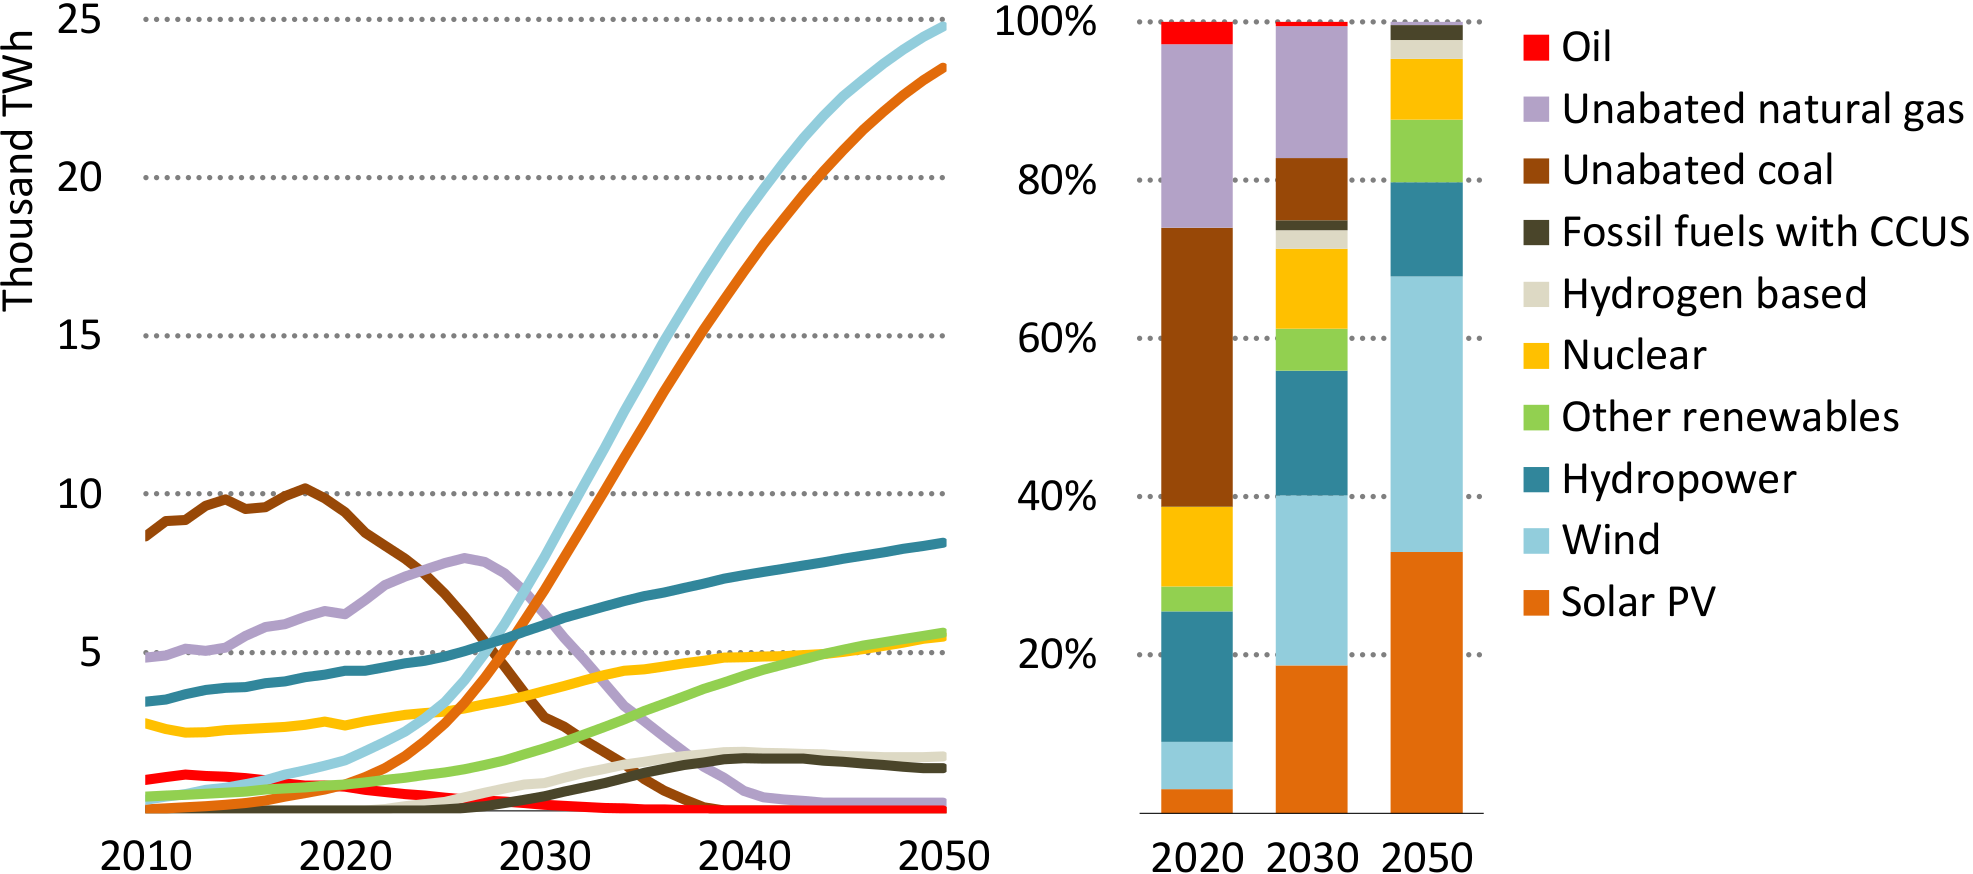
\includegraphics[width=.8\columnwidth]{2050-elec-source}
	\caption{Projected global electricity generation by source in the
	\gls{NZE}. Retrieved from \cite{iea_net_2021}.}
	\label{fig:2050-elec-source}
\end{figure}

Unlike solar or wind power, nuclear power is a dispatchable energy source; it
provides consistent and reliable power independent of weather conditions.
Beyond the electricity sector, nuclear power also has the potential to replace
fossil fuels to meet energy demands from industrial process heat applications
and transportation \cite{forsberg_market_2020}. Solar \gls{PV} and
wind are ill-suited for meeting heat demand such as district heating and
industrial heat applications at economically competitive rates. Some advanced
reactors such as \glspl{MSR} and \glspl{HTGR} operate at sufficiently
high temperatures for chemical, petrochemical, steel, and other industries.
These industries include hydrogen and ammonia production, two hydrogen-based
fuel candidates for replacing fossil fuel consumption in the aviation and
marine sectors to reduce carbon emissions.

The world would have to ramp up the current rate of reactor deployments to
replace aging reactors and displace a portion of the presently large share of
energy production from fossil fuels. However, several obstacles stand in the
way of kickstarting new reactor deployments. These obstacles include perceived
safety risks, sustainability concerns, nuclear proliferation
risks, and the ability to compete economically with other sources of energy
\cite{massachusetts_institute_of_technology_future_2003}. A potential solution
to the aforementioned issues is the \gls{MSR} concept, one of six advanced
reactor designs selected by the Generation IV International Forum
\cite{gif_technology_2002} for continued research and development.

\begin{figure}[htb!]
	\centering
	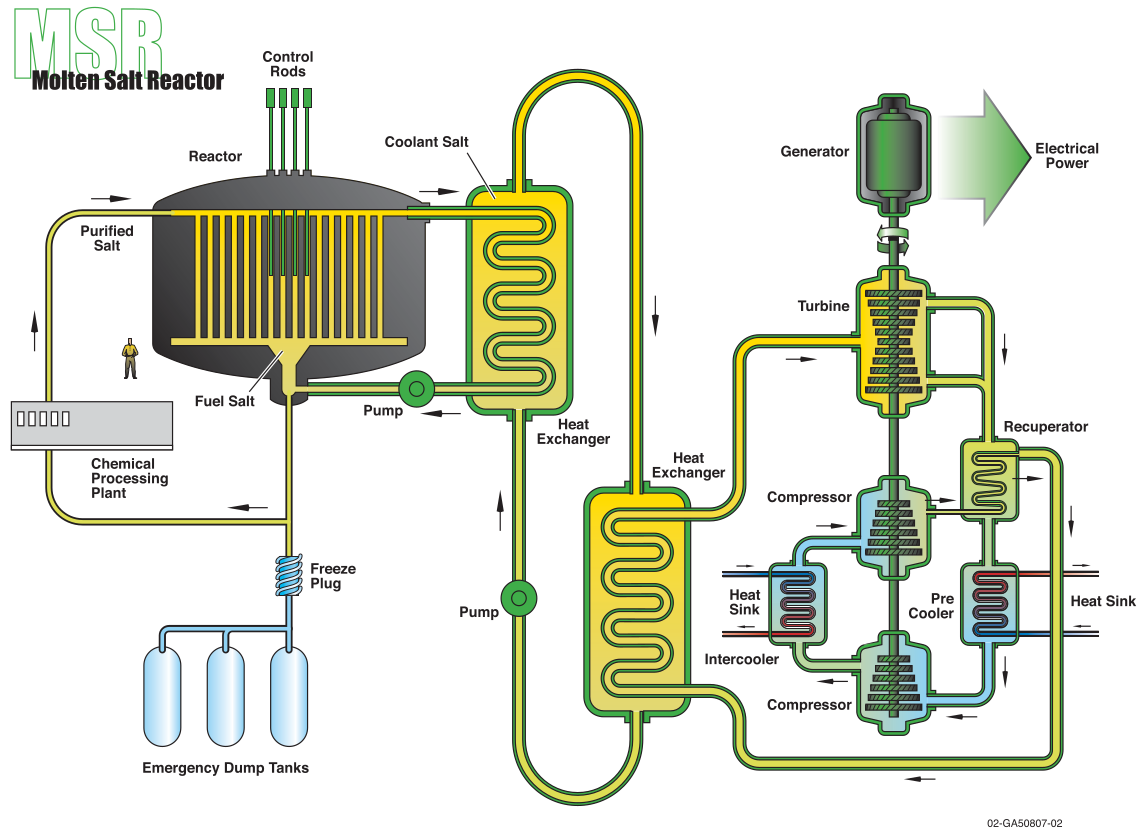
\includegraphics[width=.8\columnwidth]{msr}
	\caption{Schematic diagram of the \gls{MSR} concept. Retrieved from
	\cite{doe_technology_2002}.}
	\label{fig:msr}
\end{figure}

``\glspl{MSR}'' generally refer to all reactor designs that use molten salt as
the primary coolant. In practice, the term usually refers to liquid-fueled
designs which have fissile and/or fertile materials dissolved directly in the
molten salt coolant, whereas solid-fueled designs are commonly referred to as
\glspl{FHR}. Figure \ref{fig:msr} shows a schematic diagram of a liquid
fuel \gls{MSR} which has fissile and/or fertile materials dissolved directly in
the coolants. Liquid fuel \gls{MSR} designs possess an inherently robust
safety feature in the strongly negative fuel temperature coefficient of
reactivity \cite{elsheikh_safety_2013}. This reactivity coefficient limits the
maximum temperature that the reactor core would experience in an accident
scenario such as an unprotected reactivity insertion because the subsequent
rise in core temperatures induces a significant drop in reactivity which
quickly neutralizes the initial reactivity insertion. \glspl{MSR} also
operate at a large thermal margin to boiling and can rely on natural
circulation in the event of a pump failure. As a last resort, some \gls{MSR}
designs incorporate a drain plug consisting of air-cooled frozen salt which
melts when the core temperatures exceed a safety threshold. The hot molten salt
in the core flows down to drain tanks designed to hold the fuel-filled salt in
a subcritical configuration to halt any further chain fission reactions.
Some designs are envisioned to
incorporate the thorium fuel cycle for improved sustainability arising from the
use of abundant natural thorium resources and reduced transuranic waste
\cite{heuer_towards_2014}. The latter consequence also reduces economical costs
associated with long-term nuclear waste storage. In addition, the ability to
operate at near atmospheric pressures eliminates the need for a thick pressure
vessel and drives down construction costs, while online fuel reprocessing
reduces reactor downtime during reactor operation.

However, the liquid fuel form also brings about new computational
challenges in simulating the transient behavior of \glspl{MSR}. \glspl{MSR}
feature strong negative reactivity feedback in the primary coolant which holds
the dissolved fissile material. The feedback causes strong and
near-instantaneous interactions between reactor power and thermal hydraulic
temperature profile. Furthermore, fissile material
and \glspl{DNP} in \glspl{MSR} flow freely within the primary coolant
loop as opposed to being held in place in solid-fuel reactors. The movement of
\glspl{DNP} impacts the effective delayed neutron fraction in the core and
consequently also impacts the transient behavior of the reactor. Therefore,
\gls{MSR} computational models require robust coupling techniques to accurately
capture the strong multiphysics interactions.

Most reactor analysis applications are usually reactor-specific by
design such as TRACE \cite{nrc_trace_2007} for \glspl{LWR}, and
SAS4A/SASSYS-1 \cite{fanning_sas4a/sassys-1_2017} for
liquid metal cooled reactors. Thus, these applications would disregard
\gls{MSR}-specific phenomena and are inappropriate for \gls{MSR}
analysis without modifications to the source code. Some research efforts
do focus on adapting these applications for \gls{MSR} analysis. Examples
include the coupling of modified versions of TRACE and PARCS
\cite{pettersen_coupled_2016}, and the development of VERA-MSR from the
integrated \gls{LWR} simulation tool VERA \cite{graham_development_2019}.
Others developed their \gls{MSR} simulation tools from general
multiphysics or \gls{CFD} applications such as COMSOL
\cite{fiorina_modelling_2014} and OpenFOAM \cite{aufiero_development_2014}.

Similarly, Moltres \cite{lindsay_introduction_2018} is an open-source MSR
simulation tool built in the \gls{MOOSE} \cite{gaston_physics-based_2015}
parallel finite element framework. Lindsay et al.
\cite{lindsay_introduction_2018} first presented the tool in 2017 and
demonstrated its capabilities by simulating 2-D and 3-D models of the
\gls{MSRE}. The results showed good qualitative
agreement with the original design calculations by \gls{MSRE} researchers at
\gls{ORNL}. This thesis presents some of the new developments in Moltres
allowing for more complex and accurate \gls{MSR} simulations.

\section{Objectives}

This thesis demonstrates latest capabilities of Moltres
\cite{lindsay_introduction_2018}.
In particular, this thesis presents two more recent
developments in Moltres, namely fully integrating \gls{MOOSE}'s incompressible
Navier-Stokes module into Moltres, and introducing a
decay heat model.
The main objective of this thesis is to verify Moltres'
latest capabilities in modeling multiphysics, steady-state, and transient
behavior of fast-spectrum \glspl{MSR} through the study of the \gls{MSFR}
concept. Code-to-code verification is an important exercise in software
development for ensuring that the application produces accurate and reliable
results. This thesis covers the \gls{MSFR} concept mainly because it has been
studied extensively with readily available data in the literature to verify
against. The \gls{MSFR} design also features interesting flow
patterns that greatly affect the steady-state and transient behavior. This
present work will first present a verification of Moltres' \gls{MSFR}
diffusion neutronics against the Monte Carlo neutron transport software
Serpent 2, followed by a verification of
the coupled neutronics/thermal-hydraulics steady-state and accident transient
results against two sets of results published by
Fiorina et al. \cite{fiorina_modelling_2014}. The two sets of results arose
from a collaborative benchmarking exercise by researchers at Politecnico di
Milano and Technical University of Delft with two separate \gls{MSR}
simulation tools. Section \ref{sec:litrev} discusses these tools
in greater detail. The
secondary objective is to identify areas of improvement in Moltres for future
development.

\section{Thesis Outline}

The outline of this thesis is as follows. Chapter 2 discusses the history and
features of \glspl{MSR}, and a literature review of existing \gls{MSR}
simulation tools. The chapter also covers the \gls{MSFR} concept in greater
detail. Chapter 3 details the software and the general modeling
approach for generating the results in this thesis. Chapter 4 provides a
neutronics assessment by comparing key neutronics parameters from Moltres'
eigenvalue calculations to Serpent's Monte Carlo calculations. Chapter 5
presents steady-state results of coupled neutronics/thermal-hydraulics
\gls{MSFR} simulations in Moltres. Chapter 6 presents accident transient
simulation results for unprotected reactivity insertions, unprotected loss of
heat sink, unprotected loss of flow, and unprotected pump overspeed. Lastly,
Chapter 7 summarizes the key findings in this thesis
and posits some potential avenues for future work.

\glsresetall

\chapter{Molten Salt Reactor Multiphysics Modeling}
\label{chap:lit}
\glspl{MSR} possess unique characteristics which render existing \gls{LWR}
analysis software inappropriate for \gls{MSR} analysis. Legacy \gls{LWR}
software typically scale poorly on modern high-performance computing
clusters and do not support complex geometries beyond regular \gls{LWR} fuel
assembly lattices. Furthermore, \glspl{MSR} feature strong multiphysics
coupling which force segregated solvers into taking smaller timesteps to
maintain accuracy. This chapter provides a brief history of \glspl{MSR}
development and operation, followed by a discussion of the challenges in
\gls{MSR} multiphysics modeling
for reactor accident analysis. Next, this chapter presents a literature
review of existing multiphysics simulation software developed for \glspl{MSR}
analysis. This work focuses on software for analysing short-term reactor
dynamics which requires the ability to accurately simulate various transient
scenarios such as reactor start-up and coast-down, load-following operations,
steady-state operation, and accident analysis. Long-term dynamics such as fuel
burnup and structural corrosion fall outside the scope of this work. Lastly,
this chapter provides a literature review of turbulence modeling and control
rod modeling, and their relevance in \glspl{MSR} modeling.

\section{Historical Molten Salt Reactor Development and Operation}

\subsection{Conceptualization and Proof-of-Concept}

\gls{ORNL} researchers first conceived the \gls{MSR} concept in pursuit of a
liquid fuel reactor for the US Aircraft Nuclear Propulsion program in
the 1950s \cite{rosenthal_molten-salt_1970}. Due to high temperature
requirements, water-cooled reactors were not suitable as aircraft jet engines
\cite{dolan_1_2017}. Instead, the researchers selected molten fluoride
salts in particular for high uranium solubility, chemical stability, low vapor
pressure even at high temperatures, good heat transfer properties,
resistance against radiation damage, and reduced corrosive effects on some
common structural material \cite{rosenthal_molten-salt_1970}. They
subsequently built the first ever operational \gls{MSR}, 2.5 MW$_{\text{th}}$
\gls{ARE} reactor at \gls{ORNL}. The \gls{ARE}
achieved criticality on November 1954 and generated 100 MWh over nine days.
The reactor ran on enriched uranium in a molten salt mixture of NaF,
ZrF$_4$, and UF$_4$ with BeO neutron moderators. The aircraft program
ultimately never came to fruition as the development of intercontinental
ballistic missiles effectively eliminated the need for long-range
nuclear-powered bomber aircraft.

However, the successful demonstration of the \gls{ARE} spurred further
research into adapting \glspl{MSR} for civilian power generation
\cite{rosenthal_molten-salt_1970}. One key finding from the
research was that the thorium fuel cycle had a better breeding ratio than the
$^{238}$U-to-$^{239}$Pu fuel cycle in thermal-spectrum reactors.
Ultimately, these efforts culminated in the design, construction, and
successful operation of the \gls{MSRE}. The \gls{MSRE} had a 8 MW$_{\text{th}}$,
graphite-moderated design with a LiF-BeF$_2$-ZrF$_4$-UF$_4$ fuel salt mixture
\cite{haubenreich_experience_1970}. In January 1969, the \gls{MSRE} became the
first reactor to run on $^{233}$U fuel bred from $^{232}$Th. Among the numerous experiments
conducted on the \gls{MSRE}, the zero-power start-up and coast-down tests
\cite{prince_zero-power_1968} and the natural circulation test \cite{briggs_molten-salt_1969}
represent the most commonly referenced tests for MSR software validation due to their
straightforward demonstrations of \gls{DNP} drift and passive cooling in an \gls{MSR}.

Building on their experience with the \gls{MSRE}, \gls{ORNL} proposed a
new program for the construction and operation of a demonstration reactor
based on the \gls{MSBR} concept that they had
developed \cite{macpherson_molten_1985}. The \gls{MSBR} is a thermal-spectrum,
single fluid reactor with fertile $^{232}$Th isotopes mixed directly into the
FLiBe molten salt for $^{233}$U breeding \cite{robertson_conceptual_1971}. Like the
\gls{MSRE}, the \gls{MSBR} relies on continuous online reprocessing to add
fertile material and remove fission product neutron poisons. Researchers
estimated the doubling time (the minimum amount of time required to produce
enough fissile material to start up another \gls{MSBR}) to be
approximately 22 years. While \gls{ORNL} failed to secure funding for the
\gls{MSBR} program, two independent
technology evaluation and design studies of the \gls{MSR} had reported
favorably on the promise of the system \cite{macpherson_molten_1985}.

\subsection{Modern MSR Research and Development}

Following a relative lull lasting until the late 20th century, researchers at \gls{CNRS} began
research into \glspl{MSR} in 1997 \cite{heuer_simulation_2010}. Starting from the \gls{MSBR}
design, they performed parametric studies on reactor safety, breeding, and other performance
metrics \cite{mathieu_thorium_2006}. They found that graphite-moderated designs required careful
consideration of the fuel-to-moderator ratio as some designs exhibited positive temperature
feedback coefficients. Safer reactor configurations generally operated at very thermalized spectra
owing to large neutron losses in the graphite, or at epithermal and fast spectra owing to
$^{232}$Th resonance capture cross sections. Combined with findings on poor breeding performance
with thermal spectra and accelerated graphite irradiation damage with fast spectra, the authors
suggested eliminating the graphite moderator to optimize both reactor safety and breeding.

Their efforts culminated in the \gls{MSFR} concept, a fast-spectrum breeder \gls{MSR}
designed to run on the thorium fuel cycle \cite{merle_optimized_2007}. As opposed to the
multi-channel design of the \gls{MSRE} and \gls{MSBR}, the \gls{MSFR} reactor core consists of a
single, large channel through which the salt flows as shown in Figure \ref{fig:msfr}. In 2008, the
Generation IV International Forum highlighted the \gls{MSFR} among other \gls{MSR} designs for
further development \cite{gif_generation_2008}. The \gls{MSFR} has also benefited from
collaborative research through three projects, the \gls{EVOL} \cite{euratom_final_2015},
\gls{SAMOFAR} \cite{kloosterman_20_2017}, and \gls{SAMOSAFER} \cite{cordis_severe_nodate} projects.
Under the \gls{EVOL} project, researchers further optimized the \gls{MSFR} design based on
neutronic and \gls{TH} safety analyses. One significant modification involved a transition
from the original straight cylinder core design to curved walls in the reactor core to facilitate
smoother fuel salt flow and prevent large eddies from forming in the core
\cite{rouch_preliminary_2014}. Large eddies create hot, swirling pockets of fuel salt which could
complicate reactor operation. For instance, changes in flow conditions, intended or otherwise,
could cause the eddies to collapse and in turn introduce a localized pocket of hot fuel salt to the
circulating fuel loop. Coupled with the strong temperature reactivity feedback in the \gls{MSFR},
reactor could experience large power fluctuations every time the hot fuel salt passes through the
core. The \gls{SAMOFAR} project, which started approximately two years after the end of the
\gls{EVOL} project, supported more comprehensive safety assessments of the reactor and the
reprocessing plant, and funded a number of experiments for validation of the \gls{MSFR}'s safety
features. The ongoing \gls{SAMOSAFER} project funds further research activities with the goal of
achieving modeling, analysis, and design improvements on various aspects of \gls{MSR} operation and
safety. Other than coupled neutronics and \gls{TH} studies, the latter two projects also
conducted research and development on molten salt chemistry \cite{rodrigues_pyrochemical_2015,
duran-klie_dynamic_2016, soucek_synthesis_2017, tosolin_synthesis_2018, tosolin_vaporization_2019},
emergency salt drain plug design optimization \cite{tano_progress_2017, giraud_development_2019,
tiberga_preliminary_2019} and fission product tracking in the molten salt coolant
\cite{kalilainen_evaporation_2020, di_ronco_eulerian_2021, di_ronco_multiphysics_2022}.
%
\begin{figure}[htb!]
	\centering
	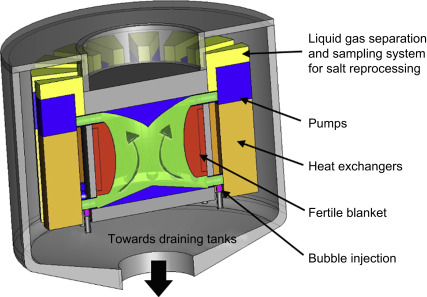
\includegraphics[width=.7\columnwidth]{msfr}
	\caption{Schematic diagram of the \gls{MSFR}. Retrieved from 
	\cite{allibert_7_2016}.}
	\label{fig:msfr}
\end{figure}

China and India have also started national programs supporting \gls{MSR} development. China
launched their \gls{TMSR} program in 2011 to develop and construct both solid-fueled and
liquid-fueled \gls{TMSR} designs \cite{zou_research_2019}. They finished construction of the 2
MW$_{\text{th}}$ TMSR-LF1 prototype in August 2021 and received approval from the Chinese Ministry
of Ecology and Environment for reactor start-up in August 2022. India also signaled their interest
especially in thorium-based reactors given their vast thorium reserves
\cite{jayaram_overview_1987}. They have developed conceptual designs of the \gls{IMSBR}, expected
to run on a fast/epithermal neutron spectrum to avoid using graphite moderators given their
tendency to deform under high neutron fluence.

In the US, Southern Company received funding from \gls{DOE}'s \gls{ARDP} \cite{doe_office_2021} to
design, construct, and operate the \gls{MCRE}, a prototype chloride salt-based \gls{MSR} similar to
TerraPower's \gls{MCFR} \cite{terrapower_mcfr_2020}, at \gls{INL}. This project builds on a prior
five-year cost-sharing project for the development of the \gls{MCFR} involving TerraPower, Southern
Company, Oak Ridge National Laboratory, Idaho National Laboratory, the Electric Power Research
Institute, and Vanderbilt University. The \gls{MCFR} is a fast-spectrum \gls{MSR} similar to the
\gls{MSFR}. Canada-based Terrestrial Energy is also developing their \gls{IMSR}
\cite{leblanc_18_2017}, a small modular \gls{MSR} based on the \gls{MSRE}. The replaceable
\gls{IMSR} core-unit which holds the reactor core, pumps, heat exchangers, and control rods, runs
for approximately 7 years before it is shut down and replaced after a cool-down period.

\subsection{Summary}

With the renewed global interest in \glspl{MSR}, \gls{MSR} modeling software play an important role
in supporting \gls{MSR} development. The \gls{ARE} and \gls{MSRE} projects first demonstrated the
feasibility of a liquid-fueled reactor with fissile fuel dissolved in molten salt coolant. The
\gls{MSBR} design features $^{233}$U breeding from $^{232}$Th with online fuel reprocessing as
opposed to infrequent batch-wise reprocessing of solid-fueled breeder reactors. The various modern
\gls{MSR} designs feature numerous changes relative to the older \gls{MSRE} and \gls{MSBR} designs
such as running on epithermal and fast neutron spectrums, different core structures, and different
molten salt compositions. However, the liquid fuel, online reprocessing capability, and other
unique features of \glspl{MSR} render many existing reactor modeling software, tailored for
modeling solid-fueled reactors, unsuitable for \gls{MSR} analysis. This fact is unsurprising
considering the dominant market share of \glspl{LWR} in the global nuclear reactor fleet, the
resultant research direction in the past few decades, and \glspl{MSR} being the sole reactor type
to utilize liquid fuel. Accurate reactor modeling capabilities are important because they
accelerate reactor design and optimization by enabling quicker iteration through numerous design
changes. \gls{MSR} modeling software are also essential tools in reactor safety analysis and
licensing efforts as reactor developers must demonstrate and verify their \gls{MSR} designs remain
safe under various accident scenarios. The next two sections provide reviews of \gls{MSR}
multiphysics modeling with respect to reactor accident analysis and control rod modeling in
\gls{MSR} multiphysics simulations.

\section{MSR Multiphysics Modeling}

This section discusses the main challenges in \gls{MSR} multiphysics modeling on reactor accident
timescales, followed by a review of existing \gls{MSR} multiphysics simulations and results in the
literature. Lastly, I present verification and validation efforts related to \gls{MSR} multiphysics
modeling.

\subsection{Challenges in MSR Multiphysics Modeling} \label{sec:challenges}

While modeling \glspl{MSR} is not necessarily more difficult than modeling
solid-fueled reactors, we must adapt our software tools to accurately model the
unique phenomena found in these circulating-fuel reactors. The differences in
the challenges of simulating \glspl{MSR} compared to solid-fueled reactors stem
mainly from the liquid fuel form of the fuel salt \cite{diamond_phenomena_2018,
huff_identifying_2019}.

Firstly, liquids generally exhibit greater thermal
expansion per unit change in temperature than solids. A decrease in density of
the fuel medium increases the likelihood of neutrons escaping the fuel region
and being absorbed by non-fissile material elsewhere in the reactor.
Consequently, combined with the temperature-dependent Doppler broadening of
resonance capture cross sections, \glspl{MSR} possess stronger negative fuel
temperature reactivity feedback than their solid-fueled counterparts
\cite{elsheikh_safety_2013}. These
phenomena ultimately result in strong interactions between the neutron fluxes
and core temperatures given that neutron fluxes affect core temperatures
through fission heat generation and core temperatures in turn affect neutron
fluxes through the mechanisms as described prior.

Secondly, with the fuel
salt also serving the role of providing cooling in the core, velocity flow
profiles in the fuel salts strongly impact the temperature distribution via
advection-dominated heat transfer \cite{diamond_phenomena_2018}. This contrasts
with the relatively static temperature profiles in fuel pins and
other forms of solid fuel matrixes physically separated from the coolant; 
changes in coolant and the resultant changes in heat transfer rates in
solid-fueled reactors are often reduced to empirical correlations governing
convective heat transfer between the fuel cladding and the coolant. On the
other hand, the velocity flow profile has a more direct effect on the
temperature distribution and the temperature-dependent neutron cross sections
in \glspl{MSR}.

Lastly, \glspl{DNP} flow freely within the primary coolant loop as opposed to
being held in place as in solid-fueled reactors. Thus, the delayed neutron
source distribution varies significantly depending on the flow profile and
velocity. In addition, the reactor loses some delayed neutrons from out-of-core
\gls{DNP} decay. These delayed neutrons are considered lost as they're emitted
in subcritical regions and are unlikely to contribute to further fission
reactions in the active core. The reduced delayed neutron fraction in the core
contributes to a greater prompt power spike following a reactivity insertion
event compared to solid-fueled reactors, absent any temperature reactivity
feedback. Thus, accurate \gls{MSR} transient simulations require accurate
modeling of \gls{DNP} drift.

The existence of multiple, disparate physics in a single system constitutes a multiphysics system.
Consequently, we need multiphysics software to accurately model a multiphysics system. Employing
well-verified single-physics software for coupled multiphysics simulations does not guarantee
stability, accuracy, or robustness \cite{keyes_multiphysics_2013}. Nevertheless, coupling separate
single-physics software for multiphysics simulations is a viable and popular option with proper
implementation. In the presence of strong coupling between different physics, extra care must be
taken to accurately capture various multiphysics interactions. For instance, the two-way coupling
between neutron flux and temperature in \glspl{MSR} described in this section necessitates robust
coupling techniques. Naive multiphysics coupling algorithms may result in longer computation times
at best and non-converging solves at worst.

Regardless of whether one couples separate single-physics software together or develops an
intrinsically multiphysics software, multiphysics software for modeling \glspl{MSR} must employ
\textit{tight coupling schemes} to couple the neutronics
and \gls{TH} governing equations to accurately capture the strong
multiphysics interactions in transient \gls{MSR} simulations. Tightly coupled
numerical models handle multiphysics interactions by either updating all state
variables simultaneously in one monolithic solve (\textit{full coupling}) or
iteratively updating all state variables (\textit{fixed point iterations})
until the solution converges in every timestep \cite{keyes_multiphysics_2013}.
Full coupling tends to be more computationally expensive because it combines
all physics equations into a single large system of equations to be solved
simultaneously, whereas fixed point iterations involve operator splitting to
separate the system of equations into smaller systems based on their associated
physics, solving smaller systems separately, and iteratively updating the state
variables until convergence. Fixed point iterative methods are often less
stable, less accurate, and have poorer
convergence rates since these methods make iterative corrections
without any regard to potentially destabilizing modes introduced by the
multiphysics coupling \cite{keyes_multiphysics_2013}. Notably, proven
techniques exist for improving the performance of fixed point iteration
coupling schemes for many relevant computational multiphysics research fields,
including reactor analysis \cite{ragusa_consistent_2009}. While fully coupled
schemes deal with solving a large system of equations, they can outperform
fixed point iterative methods in some multiphysics problems through superior
stability and convergence rates. 

In contrast to tight coupling schemes, \textit{loose coupling schemes}
solve each set of single-physics equations using state variable
data from the previous timestep without iterative corrections within every
timestep. Loosely coupled schemes are inappropriate for modeling \glspl{MSR}
given the strong coupling between the neutronics and \gls{TH}.
Aufiero et al. \cite{aufiero_development_2014} demonstrated a loose coupling
approach that failed to reproduce the expected increase in reactor power
in an \gls{MSR} in response to a 150 pcm reactivity insertion.

Consequently, MSR multiphysics simulation tools must employ, at
the very least, tight coupling schemes through fixed point iterations. The
next subsection reviews existing \gls{MSR} multiphysics simulations and results.

\subsection{Review of MSR Multiphysics Simulations and Results} \label{sec:msr-tools}

In the last two decades, several simulation tools have been developed for \gls{MSR} modeling. Given
the focus on developing high-quality \gls{MSR} software to support reactor design optimization,
this literature review omits MSR simulation work with zero-dimensional point reactor kinetics in
favor of those with spatially-resolved neutronics methods.

Most \gls{MSR} simulation tools employ tight, iterative coupling to couple separate neutronics and
\gls{TH} solvers. In 2007, Krepel et al. \cite{krepel_dyn3d-msr_2007} extended the
\gls{LWR} nodal diffusion code DYN3D to account for \gls{DNP} drift and fission energy deposition
in the coolant for \gls{MSR} modeling. The extended DYN3D-MSR code also contains the FLOCAL
\gls{TH} model for coolant flow and conjugate heat transfer modeling. Their \gls{MSRE} and
\gls{MSBR} models consisted of homogeneous hexagonal nodes (mesh elements) for the nodal diffusion
calculation coupled to individual hexagonal unit cells comprising of graphite with circular fuel
channels in the center for the \gls{TH} calculations. They simulated steady-state operation;
start-up, coast-down, and natural circulation transients; and an overcooling transient in their
\gls{MSRE} model. They also modeled steady-state operation and a single channel blockage transient
in their \gls{MSBR} model. At the \gls{TUD}, Kophazi et al. \cite{kophazi_development_2009} coupled
their in-house 3D neutron diffusion software DALTON \cite{boer_validation_2010} and \gls{TH}
software THERM to develop a 3D \gls{MSR} simulation tool. They homogenized the heterogeneous fuel
and graphite region of the \gls{MSRE} for the neutronics calculation, but they discretized the
region into a Cartesian mesh and modeled a more accurate representation of the oblong fuel channels
in the graphite core matrix as opposed to the circular shape by Krepel et al.
\cite{krepel_dyn3d-msr_2007}. Both efforts by Krepel et al. and Kophazi et al. showed good
agreement with \gls{MSRE} experimental data in their respective validation tests.
The researchers from \gls{TUD} continued in their approach of coupling separate single-physics
software to create \gls{MSR} simulation tools, as noted by the DALTON-HEAT
\cite{de_zwaan_static_2007} coupling to model the \gls{MSFR} \cite{fiorina_modelling_2014}. The
fast-spectrum \gls{MSFR} features a large pool of fuel salt in its single-channel design as opposed
to the \gls{MSRE}'s multi-channel design. As a result, the authors had to incorporate
multidimensional turbulent flow modeling to accurately model the complex flow profiles and
turbulence effects in the \gls{MSFR} during steady-state operation and transient scenarios. In a
later effort from the same institute, Tiberga et al. \cite{tiberga_discontinuous_2019} coupled
PHANTOM-$S_N$ and DGFlows in their participation in the CNRS benchmark study
\cite{tiberga_results_2020}. Developed at the \gls{CNRS}, the CNRS benchmark facilitates
code-to-code verification of \gls{MSR} multiphysics software \cite{aufiero_testing_2018}.

Another multiphysics package was developed at
the \gls{PSI} by coupling the \gls{LWR} \gls{TH} system software \gls{TRACE} \cite{nrc_trace_2007}
with the nodal neutron diffusion software \gls{PARCS} \cite{downar_parcs_2010} for a safety
analysis of the \gls{MSFR} \cite{pettersen_coupled_2016}. The straight cylinder \gls{MSFR} design
was approximated using hexagonal nodes in \gls{PARCS} while \gls{TRACE} simulated
Reynolds-averaged, inviscid coolant flow. While modeling inviscid flow reduces computational costs
by eliminating the need for expensive turbulence modeling, this approach neglects turbulent flow
and turbulent mixing effects. More recently, Jaradat et al. \cite{jaradat_development_2021}
extended the 3D $P_1$ and $SP_3$ nodal transport code PROTEUS-NODAL to support \gls{DNP} drift.
Yang et al. \cite{yang_development_2022} then developed a coupled simulation tool of PROTEUS-NODAL
and the system analysis code \gls{SAM}. They modeled the \gls{MSFR} on a 2D axisymmetric geometry
and the \gls{MSRE} on a 3D R-$\theta$-Z geometry with twelve 1D flow channels. The \gls{SAM} flow
model relied on the algebraic mixing length model for turbulence modeling. Both sets of results
reproduced the expected trends observed in published experimental and simulation data. Coupling
single-physics software to form integrated multiphysics tools allows researchers to leverage on
existing well-validated, single-physics software. These single-physics software are also highly
optimized for solving specific types of \glspl{PDE} relevant to the investigated system.

With modern advancements in computing hardware and growing access to
high-performance computing systems, others have developed multiphysics tools by
coupling the \gls{CFD} software OpenFOAM
\cite{the_openfoam_foundation_ltd_openfoam_2021} with the Monte Carlo particle
transport software Serpent \cite{leppanen_serpent_2014}, thus achieving
high-fidelity neutronics calculations in transient reactor analyses. To that end,
Serpent has a multiphysics interface supporting coupling
with other physics software \cite{leppanen_development_2013}. Laureau et al.
\cite{laureau_transient_2017} developed another technique called the
\gls{TFM} method through the introduction of additional time-dependence
operators to conventional fission matrices typically used to accelerate source
convergence in Monte Carlo neutronics calculations. The \gls{TFM} method
pre-calculates three \glspl{TFM} of the reactor system in Serpent and
interpolates the matrix values during the actual transient calculations to
incorporate temperature-induced salt expansion and Doppler
effects on the neutron cross sections and ultimately the neutron flux. Laureau et al. opted to
subcycle the neutronics calculations by setting smaller timesteps than the \gls{TH} calculations
to take advantage of the differing physics timescales. They demonstrated load-following capability
and parametric studies of overcooling and reactivity insertion transients in the \gls{MSFR}.
Blanco \cite{blanco_neutronic_2020} took a more direct approach by
compiling Serpent as an internal \texttt{C}-based function within OpenFOAM's
\texttt{C++}-based framework. This approach reduced the amount of external data
transfers between Serpent and OpenFOAM as both software have access to shared
memory during runtime. Their integrated tool employs the Quasi-Static
method for transient neutronics calculations and runs Serpent Monte Carlo
calculations several times per timestep until convergence is reached.
Blanco demonstrated the Serpent-OpenFOAM tool on the CNRS benchmark specified by Tiberga et al.
\cite{tiberga_results_2020}.

Another \gls{MSR} simulation approach involves developing inherently multiphysics software which
handle all multiphysics calculations and data transfer internally. Among earlier efforts, Nicolino
et al. \cite{nicolino_coupled_2008} and Zhang et al. \cite{zhang_development_2009} recognized the
need for more robust multiphysics coupling and acceleration techniques and internal data transfers
to reduce execution times. They each independently developed unnamed multiphysics simulation tools
and demonstrated their tools with non-moderated \gls{MSR}
designs. Later, Li et al. \cite{li_transient_2015} demonstrated the
steady-state and transient analysis capabilities of COUPLE, a neutronics and
\gls{TH} software developed at the Karlsruhe Institute of Technology.
Others adopted extensible software frameworks for developing numerical solvers
to develop multiphysics reactor analysis software. Examples of these software
frameworks include the commercial COMSOL
Multiphysics\textsuperscript{\textregistered} software
\cite{comsol_ab_comsol_nodate}, the aforementioned open-source CFD toolbox
OpenFOAM, and the open-source finite-element
framework \gls{MOOSE} \cite{gaston_physics-based_2015}. Researchers at
\gls{PoliMi} developed a \gls{MSR} simulation tool in COMSOL and
modeled the \gls{MSBR} as a single axisymmetric fuel channel with a uniform
flow profile \cite{cammi_multi-physics_2011}, followed by the \gls{MSRE} core
also as a single axisymmetric fuel channel with parabola-shaped laminar flow
\cite{cammi_dimensional_2012}. They later expanded on their approach by
modeling the \gls{MSRE} upper plenum, downcomer and lower plenum, primary heat
exchanger, and secondary heat exchanger as 0D systems (lumped-parameter model),
and substituting the 2D fuel channel with a 3D fuel channel which more closely
resembled the actual fuel channels in the \gls{MSRE}
\cite{zanetti_geometric_2015}. Other than the \gls{MSRE}, they also modeled the
\gls{MSFR} in a later publication \cite{fiorina_modelling_2014} which also featured \gls{TUD}'s
DALTON-HEAT coupled multiphysics tool.

Other institutes have dedicated significant development work towards
OpenFOAM-based \gls{MSR} simulation tools. Aufiero et al.
\cite{aufiero_development_2014} first introduced an OpenFOAM model developed
at \gls{PoliMi}. Their model implemented a neutron diffusion model and a
\gls{RANS}-based turbulence model with incompressible flow to demonstrate 2D
and 3D transient analyses of the \gls{MSFR}. Later advancements in the
\gls{PoliMi} solver include a fuel compressibility model with helium bubble
tracking to study fuel compressibility effects
\cite{cervi_development_2019} and a $SP_3$ neutron transport
model for improved neutronics calculations \cite{cervi_development_2019-1} in
the \gls{MSFR}. GeN-Foam is another OpenFOAM-based tool developed by Fiorina
et al. \cite{fiorina_gen-foam_2015} as a general reactor multiphysics solver
applicable to \glspl{MSR} and other reactor types. GeN-Foam features neutron
diffusion, $SP_3$, and $S_N$ neutronics models
\cite{fiorina_development_2016,fiorina_gen-foam_2015,fiorina_detailed_2019},
and thermo-mechanical modeling for reactor expansion effects. Using GeN-Foam,
Altahhan et al. \cite{altahhan_preliminary_2020} developed and optimized a
liquid-fuel \gls{MSR} design while Shi \& Fratoni \cite{shi_gen-foam_2021}
simulated precursor drift effects in a homogenized \gls{MSRE} model.

Finally, within the \gls{MOOSE} framework, simulation tools capable of modeling
\glspl{MSR} include: Griffin \cite{abou-jaoude_coupled_2020}; and Moltres
\cite{lindsay_moltres_2017}\textemdash the subject of this work.
Griffin primarily tackles radiation transport problems, but the \gls{MOOSE}
framework facilitates multiphysics coupling with \gls{MOOSE}-based applications for other physics
such that all applications share the same data structure. This feature eliminates
computational costs from external data transfers and optionally allowing for
\textit{fully coupled} solves in which the application solves all physics
simultaneously. The mutual compatibility among different physics applications within the
\gls{MOOSE} framework simplifies the work required to strongly couple
different physics together to solve novel multiphysics problems. Similarly,
Moltres benefits from the highly-integrated cross-compatibility
within the ecosystem of \gls{MOOSE}-based applications. Abou-Jaoude et al.
\cite{abou-jaoude_coupled_2020} coupled Griffin with Pronghorn, another
\gls{MOOSE}-based application for advanced reactor \gls{TH} modeling, to
demonstrate several steady-state \gls{MSR} simulation capabilities defined in
the CNRS benchmark. Lindsay et al.
\cite{lindsay_introduction_2018} first demonstrated Moltres' \gls{MSR} modeling
capabilities on 2D axisymmetric and 3D Cartesian models of the \gls{MSRE} with
fixed velocity flow on a fully coupled neutronics and \gls{TH} solve.
I later demonstrated some of Moltres' more recent developments through
modeling a 2D axisymmetric model of the \gls{MSFR} for steady-state operation
and transient accident analysis \cite{park_advancement_2020}. The latter study
introduced looped \gls{DNP} flow, coupling the \gls{DNP} drift and temperature 
advection-diffusion to incompressible flow, and decay heat modeling
capabilities.

\subsection{MSR Multiphysics Modeling Verification \& Validation}

\gls{VV} of simulation models are important components of simulation software development
\cite{sargent_verification_2010}. Model verification is the process of checking whether a model and
its implementation accurately represents the conceptual description and specifications. Model
validation is the process of checking whether a model is an accurate representations of the real
world within the range of its intended uses. For reactor software, model verification is commonly
performed by comparing them to other reactor software designed to run the same type of reactor
simulations. On the other hand, model validation is performed by comparing numerical results from
a simulation model to experimental data from the corresponding live test. The validity of a model
depends on the outcome of both model verification and validation.

The important multiphysics phenomena in \glspl{MSR} for model \gls{VV} are salt flow-induced
\gls{DNP} drift and the strong coupling between neutron flux and temperature advection-diffusion as
described in Subsection \ref{sec:challenges}. Delpech et al. \cite{delpech_benchmark_2003}
published one of the first modern \gls{VV} work for \gls{MSR} multiphysics modeling. Collaborators
from six institutions modeled \gls{MSRE} pump start-up, pump coast-down, and natural
circulation transients to assess and validate their models and codes for studying the effects of
salt flow on the reactivity and power. Given the wide range of neutronics methods from
multidimensional Monte Carlo methods to zero-dimensional point reactor kinetics, some deviations
were observed between different codes. Neverthless, all results showed generally good agreement
with \gls{MSRE} experimental data from \gls{ORNL}.

As mentioned in Subsection \ref{sec:msr-tools}, Tiberga et al. \cite{tiberga_results_2020}
published the CNRS benchmark for the verification of \gls{MSR} simulation tools designed for
fast-spectrum \gls{MSR} modeling. In contrast with the multi-channel \gls{MSRE} and its derivative
designs, the CNRS benchmark has a 2 m$\times$2 m problem domain of homogeneous fuel salt mimicking
the large salt pool in fast-spectrum \gls{MSR} designs. The CNRS benchmark consists of three phases
starting with single-physics calculations in Phase 0, followed by problems which gradually
introduce multiphysics coupling in Phase 1, and lastly time-dependent pertubation problems in Phase
2. Thus, the benchmark provides a systematic approach aimed towards helping code developers
identify sources of discrepancies which may otherwise be masked by error cancellation or other
dominant sources of discrepancies. The final steady-state and time-dependent problems involve
studying the effects of natural circulation and lid-driven flow on the reactivity and power output.
Aside from the problem specifications, Tiberga et al. also published the associated group
constant cross section data required by deterministic neutronics solvers to perform neutronics
calculations. Four institutions participated in the benchmarking exercise with neutron diffusion,
$SP_N$, and $S_N$-based solvers for the neutronics calculations. Their measured neutronics and
\gls{TH} parameters showed excellent agreement within up to 2.5\% discrepancy from their combined
average.

Neutronic benchmark studies of the \gls{MSRE} and the \gls{MSFR} by Fratoni et al.
\cite{fratoni_molten_2020} and Brovchenko et al. \cite{brovchenko_neutronic_2019} measured the
delayed neutron losses due to the decay of \glspl{DNP} flowing out of the active core region.
Fratoni et al. sought to establish a standard validation platform for \gls{MSR} neutronics
simulation tools with \gls{MSRE} experimental data for inclusion in the \gls{IRPhEP} handbook.
They characterized and validated a model of the \gls{MSRE} in the Monte Carlo particle transport
code Serpent. On the other hand, the \gls{MSFR} benchmark by Brovchenko et al. featured results
from multiple \gls{MSR} simulation tools by several collaborators. Their assessment found that
the choice of nuclear database for the cross sections and decay data has the most significant
impact on the neutronics results.

While these publications have plugged significant technical gaps, more can be done to develop
open \gls{VV} procedures for \gls{MSR} multiphysics modeling. For instance, the
CNRS benchmark does not assess the loss of delayed neutrons due to the decay of \glspl{DNP} flowing
out of the active core region. This phenomenon is important as the delayed neutron fraction in the
core directly impacts the transient power response in unprotected accident scenarios. Meanwhile,
the neutronic benchmark studies by Fratoni et al. \cite{fratoni_molten_2020} and Brovchenko et al.
\cite{brovchenko_neutronic_2019} did not provide standardized group constant data required by most
deterministic multiphysics \gls{MSR} simulation tools. Therefore, it is difficult to isolate
discrepancies arising from code implementations as opposed to discrepancies from using different
nuclear databases or stochastic uncertainties in Monte Carlo simulations. A good model verification
procedure for delayed neutron loss should ideally provide well-defined problems and the necessary
input data. It is also helpful to perform model verification studies on simpler problems like the
bare homogeneous problem domain in the CNRS benchmark before embarking on more complicated
validation studies which require accurate models of the reference experiments.

\section{Turbulence Modeling in MSRs}

In fluid dynamics, turbulent flow is characterized by unsteady, irregular, and
chaotic fluid motion as opposed to neat, parallel flow layers in laminar flow
\cite{pope_turbulent_2000}. The transition from laminar to turbulent flow
typically occur at Reynolds numbers between 2000 and 4000, depending on the
setup \cite{pope_turbulent_2000}. Turbulent flows are expected in \glspl{MSR}.
Kedl \cite{kedl_fluid_1970} reports expected Reynolds numbers in the \gls{MSRE}
ranging from 1000 in the regular fuel coolant channels to over 10000 in the
flow distributor volute and core wall cooling annulus regions. For the
\gls{MSFR}, salt flow in the central core region is highly turbulent and
reaches Reynolds numbers on the order of $10^5$.

\subsection{Turbulence Models}

Numerous types of turbulence models exist for various turbulent flow
applications. The most common turbulence models can be classified into the
following categories by order of increasing computational complexity:
%
\begin{itemize}
    \item \gls{RANS}-based models
    \begin{itemize}
        \item Eddy viscosity models
        \begin{itemize}
            \item Algebraic models
            \item One- and two-equation models
        \end{itemize}
        \item \gls{RSM}
    \end{itemize}
    \item \gls{DES}
    \item \gls{LES}
    \item \gls{DNS}
\end{itemize}

\gls{RANS}-based models are based on the \gls{RANS} equations obtained from
applying time-averaging to the equations of fluid flow. The \gls{RANS}
equations separate flow into time-averaged $U$ and fluctuating $u$ components
and can be writtin in Einstein notation and Cartesian coordinates as:
%
\begin{align}
    \frac{\partial U_i}{\partial t} + U_j \frac{\partial u_i}{\partial x_j} =&
    -\frac{1}{\rho} \frac{\partial P}{\partial x_i} + \nu \nabla^2 U_i -
    \frac{\partial \langle u_i u_j \rangle}{x_j}
    \shortintertext{where}
    \langle \cdot \rangle =& \mbox{ time-averaging operator,} \nonumber \\
    \rho =& \mbox{ fluid density,} \nonumber \\
    P =& \mbox{ time-averaged pressure field,} \nonumber \\
    \nu =& \mbox{ kinematic viscosity.} \nonumber
\end{align}

Eddy viscosity models, which comprise of the most widely used turbulence models
in use today \cite{rodi_turbulence_2017}, operate on the eddy viscosity
hypothesis which states that the Reynolds stresses in the \gls{RANS} equations
are given by:
%
\begin{align}
    \langle u_iu_j \rangle =& \frac{2}{3}k \delta_{ij} - \nu_T \left(
    \frac{\partial U_i}{\partial x_j} + \frac{\partial U_j}{\partial x_i}
    \right)
    \shortintertext{where}
    k =& \mbox{ mean turbulent kinetic energy,} \nonumber \\
    \delta_{ij} =& \mbox{ Kronecker delta,} \nonumber \\
    \nu_T =& \mbox{ eddy viscosity.} \nonumber \\
\end{align}

The various eddy viscosity models mainly differ in their approach towards
the closure problem of calculating the eddy viscosity. As the name suggests,
algebraic models rely on algebraic equations to calculate the eddy viscosity
distribution directly from flow variables. As a result, algebraic models are
the least computationally intensive models for turbulence. Algebraic models
can be further categorized into two types: uniform eddy viscosity models
and mixing length models. Uniform eddy viscosity models apply a uniform eddy
viscosity throughout the problem domain. The uniform eddy viscosity is
calculated from flow parameters such as the characteristic velocity, the
characteristic flow width, and empirically determined turbulent Reynolds
number. Given that eddy viscosities usually vary significantly in most types of
flow, uniform eddy viscosity models have a very limited range of applicability
\cite{pope_turbulent_2000}. Mixing length models add a level of complexity by
relating the eddy viscosity to spatially-varying flow parameters such as the
mean velocity gradient (Prandtl \cite{prandtl_7_1925} and Cebeci-Smith
\cite{smith_numerical_1967} models) or the mean rate of strain (Baldwin-Lomax
\cite{baldwin_thin-layer_1978} model) and an empirical mixing length parameter.
Combined with empirical data for the mixing length parameter, these
models provide better approximations of free shear flows, but still
underperform for more complex flows involving flow separation and significant streamline curvature.

One- and two-equation turbulence models introduce differential equations to
describing turbulence quantities such as the turbulence kinetic energy and the
turbulence rate of dissipation to obtain the eddy viscosity distribution. The
most common and best performing one-equation model is the Spalart-Allmaras
model which provides an equation for the eddy viscosity directly with several
closure coefficients and functions \cite{wilcox_turbulence_2006}. The
Spalart-Allmaras model is considered ``complete'' as it does not involve any
adjustable coefficients or functions. Calibrated for free shear flows in
aeronautical applications, the model performs modestly better than algebraic
models in these applications \cite{pope_turbulent_2000}, but it still deviates
significantly from experimental data
for separated flows \cite{wilcox_turbulence_2006}.

Investigations with
one-equation models reveal the need for an extra equation to account for
turbulent length scales separately from turbulent velocity. Thus, two-equation
models became the most widely adopted turbulence model in the late 20th century
\cite{pope_turbulent_2000}. Two-equation models include the $k$-$\epsilon$,
$k$-$\omega$, and $k$-$\tau$ models. The variables $k$, $\epsilon$, $\omega$,
and $\tau$ correspond to turbulent kinetic energy, turbulent dissipation,
specific turbulent dissipation rate, and turbulent time scale, respectively.
While none of these models perform universally well, they are generally more
accurate than the algebraic and one-equation models. Successive contributions
and modifications to the two-equation models through the years have also
improved their performance in predicting various types of turbulent flow. Their
moderate computational expense compared to expensive, high-fidelity turbulence
models favor their adoption in most commercial \gls{CFD} software for
engineering applications \cite{pope_turbulent_2000}.

\glspl{RSM} directly computes the individual components $\langle u_i u_j
\rangle$ of the Reynolds stress tensor instead of approximating it with a
single, isotropic eddy viscosity term. As a consequence, \glspl{RSM} provide
more realistic predictions for flows with significant rotational motion and
sudden changes in the mean strain rate, albeit at greater computational
expense, compared to the one- and two-equation models
\cite{wilcox_turbulence_2006}. Smaller improvements are observed in modeling
free shear flows and backward-facing step flows \cite{wilcox_turbulence_2006}.

Due to the much higher computational cost for \gls{DES}, \gls{LES}, and
\gls{DNS}, these models have limited applicability in routine, high-Reynolds
number engineering problems today. However, given their high accuracy, these
models are useful for flow problems with relatively simple geometries and at
low Reynolds numbers and validating the lower-fidelity turbulence models
\cite{zhiyin_large-eddy_2015}.

\subsection{Turbulence Modeling in MSR Simulation Tools}

For MSR modeling, the $k$-$\epsilon$ and $k$-$\omega$ turbulence models are the
most commonly used models as shown in published work with COMSOL
\cite{fiorina_modelling_2014}, OpenFOAM \cite{aufiero_development_2014}, and
\gls{TUD}'s in-house codes \cite{fiorina_modelling_2014,tiberga_results_2020}.
Podila et al. \cite{podila_cfd_2019} performed \gls{CFD} simulations of the
\gls{MSRE} core with six different turbulence models, namely a Spalart-Allmaras
model, two variants of the $k$-$\epsilon$ model, a $k$-$\omega$ model, and two
variants of \glspl{RSM}. Their results showed relatively small differences
in graphite and fuel temperatures among different turbulence models. However,
they observed significant differences in the turbulence intensities near the
wall. Given the lack of experimental data for model validation, the authors
could not make a clear assessment of the models' accuracies. Nevertheless, the
close agreement of the fuel temperatures imply that the discrepancies in the
turbulent intensities near the wall have a negligible impact on the overall
distribution of advected quantities in the \gls{MSRE}. Podila et al.
\cite{podila_cfd_2019} opted to use a $k$-$\epsilon$ model for subsequent
calculations in their work given its lowest computational cost amongst the
two-equation models and the close agreement in the temperature distributions.

Amongst other \gls{MSR} simulation tools, the $k$-$\epsilon$ and $k$-$\omega$
turbulence models are the most commonly used models as shown in published work
with COMSOL \cite{fiorina_modelling_2014}, OpenFOAM
\cite{aufiero_development_2014}, and \gls{TUD}'s in-house codes
\cite{fiorina_modelling_2014,tiberga_results_2020}. Fiorina et al.
\cite{fiorina_modelling_2014} compared the flow distribution from both models
in a 2D axisymmetric \gls{MSFR} geometry and observed that the $k$-$\omega$
model produced a wider recirculation zone near the outer wall, an additional
recirculation zone near the top wall, and significantly higher maximum
temperatures within the former recirculation zone. In a recent study by
Laureau et al. \cite{laureau_unmoderated_2022}, the authors applied a \gls{DES} model to model
eddies in the \gls{MSFR}. Given the high computational costs required to obtain reasonably small
stochastic uncertainties from Monte Carlo calculations on arbitrarily varying temperature fields,
they created a reduced order model relating local reactivity feedback estimates to the nominal
temperature field to obtain the effective temperature field. Additionally, they fixed the total
reactor power output to 3 GW to further reduce costs. With this multiphysics model, they found
the pre-existing \gls{MSFR} model was prone to large power fluctuations up to 7.5\% under
steady-state operation. Previous studies with lower-fidelity models, including the two-equation
models, failed to capture this effect due to the time-averaging assumption required in those
models. After replacing the large inlet pipes with multiple blade-like inlet channels in the
\gls{MSFR} model, they managed to reduce power fluctuations to 1.2\%.

In essence, the existing literature on turbulence flows in \glspl{MSR} work highlight
the importance of modeling turbulent flows and calls for extra care towards the choice of
turbulence model depending on the \glspl{MSR} design and the phenomenon being studied.

\section{Control Rod Modeling in MSRs}

\subsection{Control Rods in MSRs}

Most reactor designs have control rods to control the fission rate or completely shut down the
reactor by inserting the rods further into the reactor core. As such, control rods consist of
strong neutron absorbers like boron, cadmium, and gadolinium to reduce the number of fission
neutrons available to contribute to further fission chain reactions. All reactors start operation
with excess reactivity to ensure that they have enough fissile material to last through to the next
scheduled refueling. Control rods, along with burnable poisons, allow reactors to operate at a
multiplication factor of unity by canceling out the excess reactivity. Control rods are also useful
for ramping the power up or down during start-up, shut-down, or load-following operations. Most
importantly, control rods provide a safety mechanism for quickly shutting down a reactor under
dangerous conditions. Rapid control rod insertion is the main mechanism of a reactor scram to
reliably introduce a large negative reactivity insertion in response to an unintended reactivity
insertion or other events which may threaten the safe operation of the reactor. 

The number and locations of control rods in a reactor vary significantly for different reactor
types, depending on their maximum operating power, refueling frequency, and other factors. For
instance, as shown in Figure *, a single fuel assembly in a \gls{PWR} can accommodate 24 control
rods in close proximity to the fuel pins. The total number of fuel assemblies vary from 37
assemblies in the NuScale VOYGR reactor to 157 assemblies in the Westinghouse AP1000 reactor. On
the other hand, the entire MHTGR-350 high-temperature gas reactor, shown in Figure *, has 30
control rods in total. The control rods are located in graphite reflector blocks, thereby placing
them further from fuel elements. Lastly, the \gls{MSRE} design has three control rods located
centrally in graphite-moderated core with fuel salt channels.

[Insert control rod illustration]

There is a notable lack of research efforts into improving control rod modeling in \glspl{MSR}.
The self-regulating nature and low excess reactivity of \glspl{MSR} reduces or even eliminates the
need for control rods \cite{dolan_1_2017}. This characteristic arises from the strongly negative
temperature reactivity feedback and the strong coupling to flow and heat removal rates. \gls{MSR}
reactor designers rely on these passive mechanisms for reactor safety. In addition, they propose
load-following operation by adjusting pump speeds and the temperature of the intermediate coolant
loop. Laureau et al. \cite{laureau_transient_2017} demonstrated simple power ramp-up and ramp-down
with the \gls{MSFR} by varying the temperature of the secondary coolant. Examples of \gls{MSR}
designs with no control rods include the fast-spectrum \gls{MSFR} and TerraPower's \gls{MCFR}
\cite{terrapower_terrapower_2021}. However, \gls{MSR} power control schemes which rely heavily on
these mechanisms may not be suitable for all accident scenarios. Control rod insertion can provide
an additional means of reactor shutdown without resorting to draining the fuel salt and
complicating reactor restart procedures. We also note that thermal \gls{MSR} designs like the
\gls{MSRE}, \gls{MSBR}, and TMSR-LF1 designs still include control rods as essential components in
their designs, partly due to their less negative temperature reactivity feedback coefficients
compared to their fast-spectrum counterparts. Thus, the existing literature on control rod modeling
in \glspl{MSR} are based on thermal-spectrum \glspl{MSR}.

Few \gls{MSR} multiphysics studies explicitly include control rods in their models. For instance,
for the \gls{MSRE} pump start-up and coast-down experiments at \gls{ORNL} which involved control
rod movement, most numerical studies simulate the reactivity effects of the control rods by scaling
the neutron source term by the neutron multiplication factor to keep their reactor model at
criticality \cite{delpech_benchmark_2003, krepel_dyn3d-msr_2007}. Some studies include control rod
models in their steady-state calculations, but they resort to neutron source term scaling for the
transient calculations due to the inaccuracy of neutron diffusion, $P_1$, and $SP_N$ methods in
highly neutron absorbing regions \cite{kophazi_development_2009, jaradat_development_2021,
yang_development_2022}. Kophazi et al. \cite{kophazi_development_2009} modeled annular control rods
as homogenized hexahedrals in their 3D Cartesian geometry of the \gls{MSRE}. They
homogenized fuel and graphite regions in the rest of the reactor model as mentioned in Subsection
\ref{sec:msr-tools}. To reduce errors introduced by the neutron diffusion method, they imposed
simple albedo boundary conditions for the thermal neutron group. Jaradat et al.
\cite{jaradat_development_2021} and Yang et al. \cite{yang_development_2022} modeled the \gls{MSRE}
control rods as homogenized wedges in their R-$\theta$-Z mesh due to the constraints of the nodal
neutronics solver. Cui et al. \cite{cui_development_2021} also homogenized the control rods as
regular hexahedral nodes in accordance to their nodal solver in Cartesian geometry. A disadvantage
of homogenization-based methods is that it removes some of the heterogeneity in the flux and
temperature. The heterogeneous temperature distribution is especially important in \glspl{MSR} due
to the collocation of fuel and coolant, and the positive temperature reactivity feedback observed
in graphite under certain conditions \cite{mathieu_thorium_2006}.

[Insert figures of the control rod models by Kophazi, Jaradat, \& Cui]

In theory, multiphysics simulation tools with Monte Carlo neutron transport such as the
Serpent-OpenFOAM tool developed by Blanco \cite{blanco_neutronic_2020} could boast excellent
control rod modeling performance. However, the computational cost would be extremely high for
reactor geometries much more complex than the 2 m$\times$2 m homogeneous domain of the CNRS
benchmark (Subsection \ref{sec:msr-tools}). Other high-fidelity neutronics methods such as the
$S_N$ and $P_N$ methods are also typically too computationally expensive for time-dependent
multiphysics simulations. On the other hand, less taxing methods such as the neutron diffusion
method cannot model control rods accurately. The remainder of this section describes the challenges
of control rod modeling with neutron diffusion, and reviews existing transport correction
techniques for improving neutron diffusion method performance in control rod modeling.

\subsection{Challenges in Control Rod Modeling} \label{sec:challenges-control-rod}

In reactor design, we aim to determine control rod worth which is measured as the reduction
in the neutron multiplication factor $k_{eff}$ due to the presence of the control rod in the
reactor. We are also interested in the accompanying change in flux shape in the vicinity of the
control rod. Neutrons entering the control rods have a higher chance of being absorbed than
adjacent regions in the reactor core. Therefore, control rods induce highly anisotropic neutron
angular fluxes and sharp gradients in the neutron flux in their vicinity. Control rods also cause
shifts in the neutron energy spectrum because their absorption cross sections are much higher in
the lower neutron energy range; more energetic neutrons generally have a higher probability of
escaping the control rod region. As a consequence, modeling control rods accurately requires
high-fidelity computational methods to capture the angular- and energy-dependence in the neutron
flux near the highly absorbing medium.

High-fidelity \textit{neutron transport methods} fall under two categories: stochastic Monte Carlo
methods and deterministic methods. Monte Carlo methods involve simulating a finite number of
neutron histories. Randomly generated numbers determine the outcome of various probabilistic events
such as travel distances between particle collisions, types of collisions, and scattering angles in
each history until it is terminated by a neutron capture event. Deterministic methods for neutron
transport, such as the discrete ordinates $S_N$ and spherical harmonics $P_N$ methods, solve the
\gls{BTE} for neutron transport with some approximations for handling the angular and energy
dependence. The \gls{BTE} for neutron transport is given as:
%
\begin{align}
  \frac{1}{v(E)} \frac{\partial}{\partial t} \Psi(\vec{r},E,\hat{\Omega},&t) + \hat{\Omega}\cdot
  \nabla\Psi(\vec{r},E,\hat{\Omega},t) + \Sigma_t(\vec{r},E,t)\Psi(\vec{r},E,\hat{\Omega},t) 
  \nonumber \\
  - \int^\infty_0 dE'& \int_{4\pi} d\hat{\Omega}' \Sigma_s(\vec{r},E'\rightarrow E,\hat{\Omega}'
  \rightarrow \hat{\Omega},t) \Psi(\vec{r},E',\hat{\Omega}',t) \nonumber \\
  =& \frac{\chi(E)}{4\pi}
  \int^\infty_0 dE' \int_{4\pi} d\hat{\Omega}' \nu\Sigma_f(\vec{r},E',t) \Psi(\vec{r},E',
  \hat{\Omega}',t)+S(\vec{r},E,\hat{\Omega}',t) \label{eq:bte}
  \shortintertext{where}
  v(E) =& \mbox{ neutron velocity,} \nonumber \\
  \Psi(\vec{r},E,\hat{\Omega},t) =& \mbox{ neutron angular flux,} \nonumber \\
  \vec{r} =& \mbox{ spatial coordinates,} \nonumber \\
  E =& \mbox{ neutron energy,} \nonumber \\
  \hat{\Omega} =& \mbox{ direction of neutron travel,} \nonumber \\
  t =& \mbox{ time,} \nonumber \\
  \Sigma_t(\vec{r},E,t) =& \mbox{ macroscopic total cross section,} \nonumber \\
  \Sigma_s(\vec{r},E'\rightarrow E,\hat{\Omega}'\rightarrow \hat{\Omega},t) =&
  \mbox{ macroscopic scattering cross section,} \nonumber \\
  \chi(E) =& \mbox{ fission neutron spectrum,} \nonumber \\
  \nu =& \mbox{ number of neutrons produced per fission reaction,} \nonumber \\
  \Sigma_f(\vec{r},E',t) =& \mbox{ macroscopic fission cross section,} \nonumber \\
  S(\vec{r},E,\hat{\Omega}',t) =& \mbox{ external neutron source.} \nonumber
\end{align}

The $S_N$ method discretizes the continuous angular directional phase space into a few discrete
angular directions (ordinates) and uses quadrature rules to replace the integrals over
$\hat{\Omega}$ with summations over the ordinates. On the other hand, the $P_N$ method introduces
Legendre polynomial expansions of the angular flux to approximate the angular dependence. Both
methods require higher-order approximations, through more discrete ordinates or higher-order
Legendre expansions, to produce accurate flux solutions. Both methods also discretize the
continuous energy dependence into discrete neutron energy groups which cover non-overlapping,
finite energy ranges across the entire energy spectrum to form multigroup equations as follows:
%
\begin{align}
  \frac{1}{v_g} \frac{\partial}{\partial t} \Psi_g(\vec{r},\hat{\Omega},&t) + \hat{\Omega}\cdot
  \nabla\Psi_g(\vec{r},\hat{\Omega},t) + \Sigma_{t,g}(\vec{r},t)\Psi_g(\vec{r},\hat{\Omega},t)
  \nonumber \\
  - \sum^G_{g'=1}& \int_{4\pi} d\hat{\Omega}' \Sigma_s^{g'\rightarrow g}(\vec{r},\hat{\Omega}'
  \rightarrow \hat{\Omega},t) \Psi_{g'}(\vec{r},\hat{\Omega}',t) \nonumber \\
  =& \frac{\chi_g}{4\pi}
  \sum^G_{g'=1} \int_{4\pi} d\hat{\Omega}' \nu\Sigma_{f,g'}(\vec{r},t) \Psi_{g'}(\vec{r},
  \hat{\Omega}',t)+S_g(\vec{r},\hat{\Omega}',t) \label{eq:mg-bte}
  \shortintertext{where}
  G =& \mbox{ total number of energy groups,} \nonumber \\
  g =& \mbox{ neutron energy group index (in decreasing energy order)} = 1,2,...,G. \nonumber
\end{align}

The subscript $g$ denotes the corresponding quantity for neutrons in energy group $g$.
Overall, neutron transport methods are very computationally expensive and thus are mainly used for
time-independent neutronic analyses. For time-dependent multiphysics simulations coupling
neutronics to \gls{TH} and other physics present in nuclear reactors, most reactor codes
rely on the neutron diffusion equation for modeling neutronics. The multigroup neutron diffusion
equations are \glspl{PDE} derived from Eq. \ref{eq:mg-bte} by making
simplifying assumptions on the angular dependence in the scattering cross section and integrating
the equations over all solid angles to eliminate angular dependence as follows:
%
\begin{align}
  \frac{1}{v_g} \frac{\partial}{\partial t} \phi_g&(\vec{r},t) + \nabla\cdot J_g(\vec{r},t)
  +\Sigma_{t,g}(\vec{r},t) \phi_g(\vec{r},t) \nonumber \\
  =& \sum^G_{g'=1}\left[\Sigma_s^{g'\rightarrow g}
  \phi_{g'}(\vec{r},t) + \chi_g \nu\Sigma_{f,g'} \phi_{g'}(\vec{r},t)\right] + S_g(\vec{r},t)
  \label{eq:mg-diff} \\
  \shortintertext{where}
  J_g(\vec{r},t) =& \mbox{ neutron current for neutron group $g$.} \nonumber
\end{align}

Fick's first law of diffusion provides a closure relation for Eq. \ref{eq:mg-diff} by relating the
current to the flux:
%
\begin{align}
  J_g(\vec{r},t) =& -D_g(\vec{r},t)\nabla\phi_g(\vec{r},t) \label{eq:fick}
  \shortintertext{where}
  D_g(\vec{r},t) =& \mbox{ neutron diffusion coefficient for neutron group $g$.} \nonumber
\end{align}

The diffusion coefficient itself is estimated from the total or transport cross sections, depending
on whether we take scattering to be isotropic or linearly anisotropic in the $P_1$ approximation of
the \gls{BTE} \cite{lamarsh_introduction_1975}:
%
\begin{align}
  D(\vec{r},t) =& \frac{1}{3\Sigma_t(\vec{r},t)} \quad \mbox{(isotropic)} \\
  D(\vec{r},t) =& \frac{1}{3\Sigma_{tr}(\vec{r},t)} = \frac{1}{3\left(\Sigma_t(\vec{r},t)-
  \bar{\mu}\Sigma_s(\vec{r},t)\right)}
  \quad \mbox{(linearly anisotropic)} \label{eq:p1-diffcoef}
  \shortintertext{where}
  \Sigma_{tr} =& \mbox{ macroscopic transport cross section,} \nonumber \\
  \bar{\mu} =& \mbox{ average cosine of the scattering angles.} \nonumber
\end{align}

This treatment significantly reduces the number of coupled \glspl{PDE} to be solved and the
computational costs of modeling neutronics in reactors. Yet, the simplifications limit the validity
of the neutron diffusion equation to regions of high scattering-to-absorption ratios at least a
few mean free paths away from shared interfaces to neighboring media with highly dissimilar
neutronic properties \cite{shultis_chapter_2016}. A single diffusion constant cannot capture the
strongly anisotropic flux within and near control rod regions.

Many legacy diffusion solvers are based on coarse-mesh or nodal methods. These methods
primarily involve replacing heterogeneous lattices of materials of differing properties with
equivalent homogeneous mixtures of the same materials in each coarse mesh (referred to as nodes in
nodal methods) \cite{stacey_nuclear_2007}. Reducing the heterogeneity of the geometry reduces
computational complexity and circumvents poor diffusion performance in highly heterogeneous
interfaces. Each coarse mesh typically corresponds to a subregion comprising of repeating
substructures, e.g. a single fuel assembly or randomly distributed spherical fuel pebbles. The
homogenization procedure consists of two main steps: a transport calculation to obtain detailed
heterogeneous flux distribution within each subregion, followed by the calculation of homogenized
\textit{group constants} from the detailed flux distribution. \textit{Group constants} refer to
macroscopic neutron cross section values for various neutron interactions such as neutron
scattering, absorption, and fission. Macroscopic cross sections represent the probability that a
neutron, in a given energy range, will undergo the associated interaction per unit distance
traveled in the material. Group constants also broadly include neutron diffusion
coefficients/constants and \gls{DNP} data. While advanced coarse-mesh and nodal
methods provide reasonable flux solutions for calculating global and intermediate-scale quantities,
they do not capture detailed heterogeneous flux distribution within each coarse mesh subregion.

\subsection{Transport Correction Techniques With Neutron Diffusion-Based Solvers}

Transport correction techniques for diffusion-based solvers require additional information beyond
conventional homogenized group constants from transport-based solvers to ameliorate diffusion
solution accuracy in highly absorbing and near-interface regions.
Therefore, this literature review focuses on hybrid diffusion-transport methods developed to relay
transport corrections in the form of more accurate neutron flux and current estimates to
diffusion-based solvers. The methods differ mainly in how they incorporate corrections into a
diffusion-based solver. While the focus of this work is on improving diffusion-based control rod
modeling in Moltres for \gls{MSR}-like designs, this literature review explores existing methods
developed for other reactor types as no advanced techniques have been applied on \glspl{MSR}.

\subsubsection{Absorber Blackness and Linear Extrapolation Length}

Methods based on absorber blackness \cite{davison_influence_1951, spinks_extrapolation_1965,
pellaud_extrapolation_1968, mendelson_two-dimensional_1969} encompass a
broad class of procedures for generating boundary conditions to match approximate solutions of
low-order methods (e.g. diffusion) to more accurate solutions from high-order methods (e.g.
transport). The internal boundary conditions replace absorber regions and mimic their presence in
the problem domain. The boundary conditions are generalizations of the Marshak boundary condition
\cite{marshak_note_1947} which in 1D are of the form:
%
\begin{align}
  \frac{\phi(x)}{d\phi(x)/dx} =& \lambda \label{eq:marshak}
  \shortintertext{where}
  \lambda =& \mbox{ linear extrapolation length.} \nonumber
\end{align}
%
The gradient of the flux in the denominator is taken in the outward direction at the surface of the
absorber or black body. In Cartesian coordinates, it is common to approximate Eq. \ref{eq:marshak}
in the form:
%
\begin{align}
  \phi(x+\lambda) =& 0
\end{align}
because Dirichlet boundary conditions are easier to work with analytically and numerically.
The corresponding relations in cylindrical and spherical coordinates depend on the radius of the
absorber rod. Various forms for $\lambda$ exist for specific absorber geometries such as slabs
\cite{maynard_blackness_1959} and cylinders \cite{spinks_extrapolation_1965,
pellaud_extrapolation_1968} which were dependent
on the size of the absorber region and coefficients quantifying the escape probability of neutrons
entering the absorber region. The $\lambda$ and the associated coefficients were derived
analytically from the \gls{BTE} with some simplifying assumptions as such having uniform or
cosine-shaped incident neutron currents, isotropic scattering within the absorber, and mathematical
approximations in ignoring higher-order terms in intermediate steps. Blackness theory emerged in
the mid-20th century when computational resources were limited. Later, as computational
resources became more readily available and powerful enough for more complicated transport
calculations, appropriate boundary conditions could be calculated numerically
\cite{bretscher_computing_1997}. Alternatively, effective group constants can be calculated for
diffusion codes which are not programmed to handle internal boundary conditions. For instance,
Bretscher \cite{bretscher_computing_1997} provided formulae for effective diffusion coefficient and
absorption cross section for thin absorber slabs as a function of blackness coefficients, absorber
thickness, and mesh size.

Diffusion calculations with corrections from blackness theory can generally provide control rod
worths which are in reasonable agreement with more accurate transport calculations. However, the
diffusion flux distributions still deviate significantly from transport calculations because no
corrections are introduced in the adjacent regions near the absorber where the angular flux can be
strongly anisotropic.

\subsubsection{Method of Equivalent Cross Sections}

Scherer \& Neef developed the \gls{MECS} \cite{scherer_determination_1976} to improve control rod
modeling in \gls{HTGR} with mesh-centered nodal diffusion methods. The \gls{MECS} involves running
a 1D neutron transport calculation on a representative \textit{super cell} of the heterogeneous
absorber region and its vicinity. The super cell is a volume-preserved model of the absorber region
approximated from its cylindrical or Cartesian geometry in the diffusion solve. The transport
calculation is typically performed using a fine group structure, fine spatial discretization, and
high-order angular discretization and scattering moments (e.g. $S_8$ method with $P_3$ scattering
matrix) \cite{fen_modelling_1992}. The calculated net neutron leakage rates from the tranport
solver are matched with the calculated leakage rates from the diffusion solver according to an
analytic calculation to obtain equivalent diffusion coefficients or cross sections for the absorber
region. The diffusion coefficient formula for this analytic calculation depends on the solution
method of the diffusion solver. In the most widely used implementation of \gls{MECS} used in
conjunction with the mesh-centered diffusion code CITATION \cite{teuchert_vsop94_1994}, the
diffusion coefficient formula assumes there is only one inner mesh point in the absorber region as
using more inner mesh points greatly increases the difficulty of finding the proper analytic
formula \cite{fen_modelling_1992}. Other macroscopic cross sections for the absorber region are
calculated using conventional group constant generation techniques from the transport solution
using the super cell average flux and reaction rates. To facilitate further discussion of the
\gls{MECS}, here is an example of applying the \gls{MECS} on a control rod in x-y geometry (Figure
\ref{fig:mecs-geometry}) in the CITATION code as provided by Fen et al. \cite{fen_modelling_1992}.
%
\begin{figure}[htb!]
    \centering
    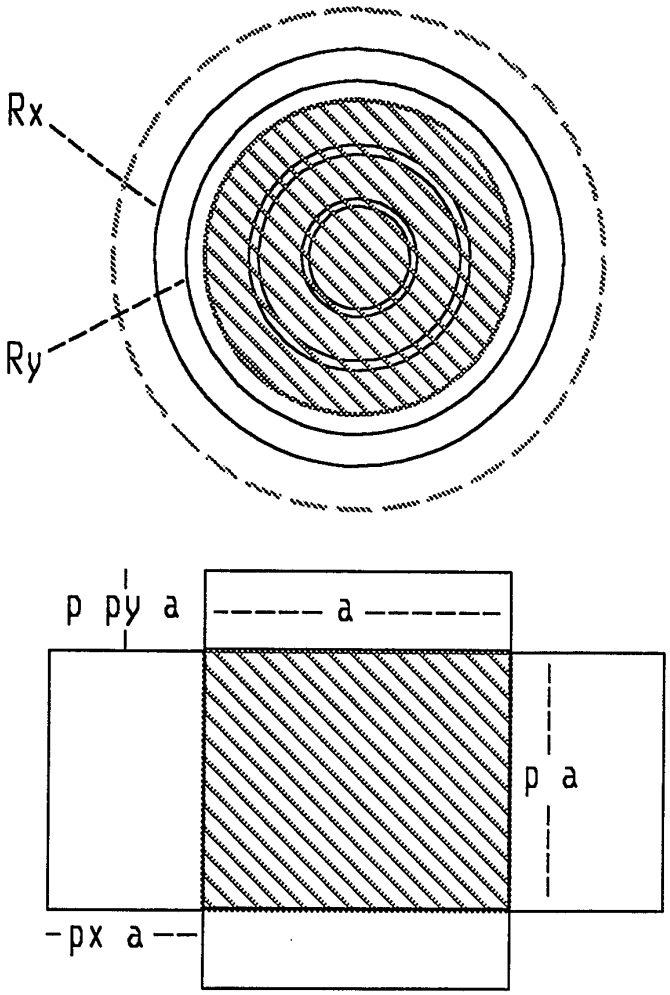
\includegraphics[width=.6\columnwidth]{mecs-geometry}
    \caption{Geometries of the absorber region and its vicinity in the super
        cell (top) and the diffusion solver mesh (bottom).
        The shaded and unshaded regions represent the homogenized absorber
        region and the adjacent non-absorber region, respectively.
        Retrieved from Fen et al. \cite{fen_modelling_1992}.}
    \label{fig:mecs-geometry}
\end{figure}

Figure \ref{fig:mecs-geometry} shows the 1D cylindrical super cell for the
transport solver on the top and the corresponding 2D Cartesian geometry for the
diffusion solver on the bottom. The four adjacent nodes in the Cartesian
geometry and their corresponding flux values are pairwise identical.

According to the mesh-centered geometry in CITATION, the leakage $L$ is
calculated as:
%
\begin{align}
  L =& \frac{F_y\left(\phi_x-\phi_a\right)}{\frac{\delta_x}{D_a}+
    \frac{\Delta_x}{D_o}} + \frac{F_x\left(\phi_y-\phi_a\right)}{
  \frac{\delta_y}{D_a}+\frac{\Delta_y}{D_o}} \label{eq:mecs}
  \shortintertext{where}
  \phi_x =& \mbox{ flux in the $x$-neighbor nodes,} \nonumber \\
  \phi_y =& \mbox{ flux in the $y$-neighbor nodes,} \nonumber \\
  \phi_a =& \mbox{ flux in the absorber node,} \nonumber \\
  F_y =& \mbox{ surface area to $y$-neighbor nodes} = 2pa, \nonumber \\
  F_x =& \mbox{ surface area to $x$-neighbor nodes} = 2a, \nonumber \\
  \delta_x =& \mbox{ distance from the absorber node center to the
    $x$-surface} = a/2, \nonumber \\
  \delta_y =& \mbox{ distance from the absorber node center to the
    $y$-surface} = pa/2, \nonumber \\
  \Delta_x =& \mbox{ distance from the $x$-surface to the $x$-neighbor node
    center} = p_x a/2, \nonumber \\
  \Delta_y =& \mbox{ distance from the $y$-surface to the $y$-neighbor node
    center} = p p_y a/2, \nonumber \\
  a, p, p_x, p_y =& \mbox{ geometric parameters of the CITATION mesh geometry
    (Figure \ref{fig:mecs-geometry}),} \nonumber \\
  D_a =& \mbox{ diffusion coefficient in the absorber node,} \nonumber \\
  D_o =& \mbox{ diffusion coefficient in the neighboring nodes.} \nonumber
\end{align}

In the original formulation by Scherer \& Neef \cite{scherer_determination_1976}, they chose to let
$D_a=D_o$. Taking leakage and flux values at $R_x$ and $R_y$ (figure \ref{fig:mecs-geometry}) from
the transport solver to be equal to the corresponding values in equation \ref{eq:mecs} yields a
value for $\phi_a$ which also represents the average flux in the absorber region. The equivalent
cross sections for each reaction type $i$ is then determined by matching reaction rates from the
transport calculation to the reaction rate as governed by diffusion theory as follows:
%
\begin{align}
  \Sigma_i =& \frac{A_i}{\phi_a V}
  \shortintertext{where}
  \Sigma_i =& \mbox{ macroscopic cross section of reaction type $i$,} \nonumber \\
  A_i =& \mbox{ reaction rate of reaction type $i$ from the transport calculation,} \nonumber \\
  V =& \mbox{ volume of the absorber region} = a^2 p.
\end{align}

Fen et al. \cite{fen_modelling_1992} later provided an updated formulation by assuming that the
cross sections are accurate and instead determined the equivalent diffusion coefficient from Eq.
\ref{eq:mecs} and the transport leakage and flux values as follows:
%
\begin{align}
  \frac{1}{D_a} =& 2p\frac{\phi_x-\phi_a}{L}+\frac{2}{p}\frac{\phi_y-\phi_a}{L}
    -\frac{p_x+p_y}{2D_o}+\sqrt{R}
  \shortintertext{where}
  R =& \left(2p\frac{\phi_x-\phi_a}{L}+\frac{2}{p}\frac{\phi_y-\phi_a}{L}+
  \frac{p_x+p_y}{2D_o}\right)^2+4p\left(p_y-p_x\right)\frac{\phi_x-\phi_a}{L}
  \frac{1}{D_o} \nonumber
\end{align}

As illustrated by the implementation in CITATION, \gls{MECS} requires considerable user input on
the super cell configuration to ensure that leakage rates of the transport solution are equivalent
to the leakage rates of the subsequent diffusion solution. This procedure also places some
constraints on the location and size of the absorber node that can be inconsistent with the
nodalization of the rest of the reactor geometry \cite{ougouag_transport_2010}. \gls{MECS} is
incompatible with reactor geometries which contain control rods that are too close to each other
such that there is not enough distance in between to define neighboring nodes where
flux-equivalence is assumed. Lastly, \gls{MECS} is only applicable to coarse-mesh solvers and
homogenizes the control rod along with the adjacent material in its vicinity. Nevertheless,
\gls{MECS} has been widely used within the \gls{VSOP}
suite of codes (which contains CITATION) and has been shown to be effective in a number of
\gls{HTGR} studies \cite{fen_modelling_1992, reitsma_evaluating_2003, mulder_neutronics_2020}.

\subsubsection{Response-Based Methods}

Similar to the \gls{MECS}, \textit{response-based methods} rely on response-function-based
transport methods to resolve the flux around absorber regions. In this context, coarse mesh/nodal
response functions relate quantities of interest of an individual node to input values from its
neighboring nodes. For instance, a response function may provide the average nodal flux and the
outgoing partial currents of a node in response to a given set of incident
partial fluxes from its neighboring nodes \cite{ougouag_transport_2010}. Transport solutions are
used to generate sets of response functions characterizing individual coarse meshes which contain
absorber regions. These response functions can be used directly or indirectly as modified boundary
conditions to accurately capture the effects of control rods on the global flux solution.

%% Delete paragraph below if not relevant
%The response-based methods described here are closely related to response-function-based transport
%methods \cite{mosher_incident_2006}, in which every node is characterized by a set of response
%functions as opposed to only generating response functions for nodes that contain absorber regions.
%The main difference lies in the accuracy and/or presence of higher order expansions of the neutron
%phase space distribution in response-function-based transport methods compared to similar
%diffusion methods. Accordingly, response-function-based transport calculations are more accurate as
%they capture more information from the reference heterogeneous transport solution for each node.

Fen et al. \cite{fen_modelling_1992} developed the \gls{RMM} which generates modified boundary
conditions from response functions to treat absorber nodes in whole core diffusion calculations.
The response functions relate the incident partial current on one face of the node to the resultant
outgoing partial currents on all four faces of the same node. To be more precise, each incident
partial current of each neutron energy group on each face may contribute to the outgoing partial
current of any energy group on any face of the same node. The following equation for the response
matrix $A$ encapsulates the response values to be generated from the \gls{RMM}:
%
\begin{align}
  A^{jk}_{nm} =& \frac{J^{+j}_n}{J^{-k}_m} \mbox{ for } j,k=1...G \mbox{ and } n,m=1...N
  \label{eq:rmm} \\
  \shortintertext{where}
  A =& \mbox{ response matrix,} \nonumber \\
  N =& \mbox{ number of spatial intervals along the perimeter of the absorber node,} \nonumber \\
  J^{-k}_m =& \mbox{ incident partial current in energy group $k$ at spatial interval $m$,}
    \nonumber \\
  J^{+j}_n =& \mbox{ outgoing partial current in energy group $j$ at spatial interval $n$}
    \nonumber \\
  &\mbox{ in response to $J^{-k}_m$.} \nonumber
\end{align}

The \gls{RMM} compares favorably against the \gls{MECS} because it captures non-isotropic flux
effects arising from the non-central control rod location within the reactor core
\cite{fen_modelling_1992}. The \gls{RMM} also does not require
meticulously tuning of thick adjacent nodes to obtain equivalent fluxes to apply the \gls{MECS}.
However, both \gls{RMM} and \gls{MECS} involve precalculation procedures which must be rerun if the
absorber region is subjected to significant changes.

Rahnema et al. \cite{rahnema_advanced_2011} later developed an \gls{IDT} method which embeds the
transport correction for absorber regions in the full-core nodal diffusion calculation. Instead of
modified boundary conditions, the \gls{IDT} method generates coupling coefficients which are
morphologically identical to those used in nodal diffusion methods. The response region, which
contains the absorber region, is further subdivided into several nodes. The transport correction
relies on higher order spatial and angular response moments to maintain detailed responses between
adjacent response nodes. Changes in the response region can be modeled by swapping out response
nodes without having to rerun the transport solver to generate new coupling coefficients. The
intra-response region calculations were iteratively coupled to the full-core diffusion calculations
to avoid introducing extra off-diagonal terms which would increase the solve time of an otherwise
tri-diagonal system of nodal diffusion equations. In several verification studies of static
\gls{HTGR} core configurations, the \gls{IDT} method produced similar eigenvalue and flux
distribution results \cite{rahnema_advanced_2011} as the \gls{RMM}. However, they did not
demonstrate the response region swapping that the \gls{IDT} was designed for.

\subsubsection{Ronen Method}

Ronen \cite{ronen_accurate_2004} postulated an alternative formulation for diffusion coefficients
based on neutron currents from transport calculations.
Fick's law of diffusion is valid under three assumptions: the neutron flux gradient is small, the
absorption-to-scattering ratio is small, and scattering sources are isotropic. Therefore, diffusion
theory fails for anisotropic fluxes in and near absorber regions. The Ronen method proposes using
the integral form of the transport equation to derive transport operators for the neutron current
and substituting the values into Fick's first law of diffusion (Eq. \ref{eq:fick}) to obtain
space-dependent diffusion coefficients as follows:
%
\begin{align}
  D(\vec{r},E) =& -\frac{J_{tr}(\vec{r},E)}{\nabla \phi(\vec{r},E)}
  \label{eq:ronen}
  \shortintertext{where}
  J_{tr} =& \mbox{ transport-derived neutron current.} \nonumber
\end{align}

In doing so, the Ronen method provides pointwise corrections to the diffusion equation which
overcome the small flux gradient limitation. Tomatis \& Dall'Osso \cite{tomatis_application_2011}
numerically implemented the Ronen method for a 1D homogeneous slab with two energy groups and
isotropic scattering. Instead of using Eq. \ref{eq:ronen} which showed instabilities near flat flux
regions where the denominator approaches zero, they calculated corrections to the diffusion
coefficients at cell interfaces using the difference between the transport- and diffusion-derived
currents as follows:
%
\begin{align}
  \delta D(x_{i+1/2},E) =& -\delta J(x_{i+1/2},E) \frac{(\Delta x_{i+1}+\Delta x_i)/2}{
  \phi(x_{i+1},E)-\phi(x_i,E)}
  \shortintertext{where}
  x_i =& \mbox{ $i$-th spatial interval,} \nonumber \\
  \delta J(x,E) =& J_{tr}(x,E) - J_D(x,E), \nonumber \\
  \Delta x_i =& \mbox{ size of $i$-th spatial interval.} \nonumber
\end{align}

They derived expressions for the transport operators for $J_{tr}$ in terms of exponential integral
functions and Legendre expansions of the angular flux.
Gross et al. \cite{gross_high-accuracy_2020} extended the derivation of the transport operators to
handle 1D heterogeneous problems in the form of fuel assemblies with fuel, water, and fuel+absorber
regions. Tomatis et al. \cite{tomatis_ronen_2021} developed new numerical implementations for 1D
slab, cylindrical, and spherical geometries by employing probabilistic treatments from the
\gls{CPM} \cite{lewis_computational_1984} for the transport operators. The authors also implemented
a solver acceleration scheme which helped with the poor convergence rate observed in the earlier
studies \cite{tomatis_application_2011, gross_high-accuracy_2020}.

The results from all three studies showed improvements in flux solutions with the Ronen method over
pure diffusion solvers in all of the test cases, particularly for a 1D heterogeneous
\gls{BWR}-based problem with isotropic scattering and strong absorption cross sections
\cite{gross_high-accuracy_2020}. The error in reactivity values for three different \gls{BWR}
configurations differed from the reference $S_16$ transport calculations by at most 62 pcm after
one hundred iterations ($1$ pcm $=10^{-5}$) . However, the demonstrations were limited to simple
1D geometries. Although the authors provided derivations for anisotropic scattering, their test
cases incorporated only isotropic scattering. The derivation of semi-analytic transport operators
for more complex reactor geometries would be a much more complicated endeavor. Furthermore, without
an accompanying solver acceleration scheme, poorly converged solutions retained significant
discrepancies near material interfaces and vacuum boundaries.

\subsubsection{Averaged Eddington Factors and High-Order Empirical Diffusion Coefficients}

In a similar vein, Pounders \& Rahnema developed two separate methods for generating
space-dependent diffusion coefficients \cite{pounders_diffusion_2009}. Both methods come with the
same caveat in requiring a priori knowledge of the flux and current. The first method, called the
\gls{AEF} method, relies on the Eddington factor, which is defined as the second angular moment of
the angular flux normalized by its zeroth moment. In 1D, the Eddington factor is given as:
%
\begin{align}
  E_g(z) =& \frac{\int^1_{-1} \mu^2\psi(z,\mu)d\mu}{\int^1_{-1} \psi(z,\mu)d\mu}
\end{align}
%
The $g$ subscript denotes the discrete neutron group index of the multigroup diffusion equations
obtained from discretizing the continuous energy variable as described in Section
\ref{sec:challenges-control-rod}. The Eddington factor features in the fist angular moment of the
1D multigroup transport equations, obtained by multiplying the transport equation throughout by
$\mu=\cos\theta$ and integrating over $\mu=-1$ to $\mu=1$:
%
\begin{align}
  \frac{d\left[E_g(z)\phi_g(z)\right]}{dz} + \Sigma_{t,g}(z)J_g(z) =& \sum^G_{g'=1}
  \Sigma^{g'\rightarrow g}_{s1}(z)J_{g'}(z) \label{eq:bte-1st-mom}
  \shortintertext{where}
  \Sigma^{g'\rightarrow g}_{s1} =& \int^1_{-1} \mu \Sigma_s d\mu \nonumber
\end{align}
%
Assuming the Eddington factor varies slowly in space, we can approximate Eq. \ref{eq:bte-1st-mom}
as:
%
\begin{align}
  E_g(z)\frac{d\bar{\phi}_g(z)}{dz} + \Sigma_{t,g}(z)\bar{J}_g(z) =& \sum^G_{g'=1}
  \Sigma^{g'\rightarrow g}_{s1}(z)\bar{J}_{g'}(z) \mbox{ for } z \in V_i \label{eq:bte-1st-est}
  \shortintertext{where}
  V_i =& \mbox{ a subvolume of the system domain.}
\end{align}
The overbars distinguish the approximate solutions of Eq. \ref{eq:bte-1st-est} from the true
solution of Eq. \ref{eq:bte-1st-mom}. From Eq. \ref{eq:bte-1st-est}, the diffusion coefficient can
be defined as:
%
\begin{align}
  D_g(z) = E_g(z)\left[\Sigma_{t,g}(z)-\sum^g_{g'=1}\Sigma^{g'\rightarrow g}_{s1}(z)
  \frac{\bar{J}_{g'}(z)}{\bar{J}_g(z)}\right]^{-1} \label{eq:diffcoef-edd}
\end{align}
By further assuming that the Eddington factors are piecewise constant in each subvolume $V_i$, the
averaged Eddington factor $E^i_g$ can be evaluated as:
%
\begin{align}
  E^i_g =& \frac{E_g(z_{i+1})\phi_g(z_{i+1})-E_g(z_i)\phi_g(z_i)}{\bar{\phi}_g(z_{i+1})-
  \bar{\phi}_g(z_i)}
  \shortintertext{where}
  z_{i+1} =& \mbox{ upper bound of subvolume $V_i$,} \nonumber \\
  z_i =& \mbox{ lower bound of subvolume $V_i$.} \nonumber
\end{align}
%
The diffusion coefficient from Eq. \ref{eq:diffcoef-edd} can then be calculated as:
%
\begin{align}
  D^{AEF}_g(z) =& E^i_g\left[\hat{\Sigma}_{t,g}-\sum^G_{g'=1}\hat{\Sigma}^{g'\rightarrow g}_{s1}
  \frac{\hat{J}_{g'}}{\hat{J}_g}\right]^{-1}
  \shortintertext{where}
  \hat{\Sigma}_{t,g} =& \frac{\int_{V_i}\Sigma_{t,g}(z)J_g(z)dz}{\int_{V_i}\bar{J}_g(z)dz},
  \nonumber \\
  \hat{\Sigma}^{g'\rightarrow g}_{s1} =& \frac{\int_{V_i}\Sigma^{g'\rightarrow g}_{s1}(z)J_{g'}(z)
  dz}{\int_{V_i}\bar{J}_{g'}(z)dz}, \nonumber \\
  \hat{J}_g =& \int_{V_i} \bar{J}_g(z)dz. \nonumber
\end{align}

The second method employs a much simpler premise in that Fick's law is assumed to be accurate with
high-order empirical diffusion coefficients that are to be determined. Given a known transport
solution, the following integration holds for a small homogeneous volume $V_i$:
%
\begin{align}
  \frac{1}{V_i}\int_{V_i}J_g(z)dV =& -\frac{1}{V_i}\int_{V_i}D_g(z)\frac{d\phi_g(z)}{dz}dV.
\end{align}
%
Taking $D_g$ to be constant in $V_i$, we may apply divergence theorem to obtain
%
\begin{align}
  \bar{J}_gV_i =& -D^i_g\int_{\partial V_i} \phi_g(z)dA
  \shortintertext{where}
  \bar{J}_g =& \mbox{ average current in $V_i$,} \nonumber \\
  \partial V_i =& \mbox{ bounding surface of $V_i$.} \nonumber
\end{align}
%
Rearranging the terms, we may obtain the empirical diffusion coefficient formulation from the
transport-derived flux and current as follows:
%
\begin{align}
  D^i_g =& -\frac{\left(z_{i+1}-z_i\right) \bar{J}_g}{\left[\phi_g(z_{i+1})-\phi_g(z_i)\right]}
  \label{eq:emp}
\end{align}
%
Both \gls{AEF} and empirical methods require the respective subvolumes $V_i$ to be small enough
for the assumptions of constant Eddington factors and diffusion coefficients to hold within $V_i$.

Both methods performed much better than with conventional diffusion coefficients derived using the
$P_1$ approximation method. For the same 1D heterogeneous \gls{BWR} problem demonstrating the prior
Ronen method \cite{gross_high-accuracy_2020} but with anisotropic scattering, the absolute errors
in $k_{eff}$ are around 100 pcm after eliminating errors associated with energy group
condensation. The error values compare favorably with the 159-683 pcm error with the $P_1$ method.
The \gls{AEF} and empirical methods also reproduced the flux distributions better with a maximum
pointwise error of 2\% as opposed to 5\% from the $P_1$ method. Similar to the Ronen method, the
\gls{AEF} and empirical methods introduce pointwise corrections with information from transport
methods. However, the present methods require a priori knowledge of the true solution or otherwise
accurate estimates from transport methods, whereas the Ronen method relies on analytical transport
operators which use diffusion flux estimates from the previous iteration to update the flux
solution. Nevertheless, the \gls{AEF} and empirical methods provide the foundation for further
development of practical, self-closing transport correction techniques.

\subsubsection{General Equivalence Theory and Superhomogenization Method}

As mentioned in Section \ref{sec:challenges-control-rod}, coarse-mesh and nodal methods homogenize
heterogeneities in reactor geometries to reduce computational costs of running full-core
simulations. Equivalence techniques which reduce spatial homogenization error are also effective
for accurately modeling the worths of control rods within fuel assemblies. The \gls{GET}
\cite{koebke_new_1980, smith_nodal_1983} and \gls{SPH} \cite{kavenoky_sph_1978,
hebert_consistent_1991} methods represent the most widely used equivalence methods for improving
the performance of diffusion calculations in homogenized \gls{LWR} models. Both methods involve
deriving additional homogenization parameters from single-assembly transport calculations with
reflective boundary conditions. Since the transport calculation step is already a prerequisite step
for generating homogenized group constants, the equivalence methods are simple to implement and
impose reasonably small additional computational costs.

Koebke \cite{koebke_new_1980} first proposed abandoning continuous surface fluxes in favor of
preserving net surface currents through discontinuity factors. Smith \cite{smith_assembly_1986}
later extended this concept for assembly-homogenized calculations. The discontinuity factors are
calculated for each face of the homogenized region to preserve volumetric reaction rates and
surface neutron currents. The discontinuity factors are calculated as follows:
%
\begin{align}
  DF =& \frac{\phi^{het,sur}}{\phi^{hom,sur}}
  \shortintertext{where}
  DF =& \mbox{ discontinuity factor,} \nonumber \\
  \phi^{het,sur} =& \mbox{ surface flux of the region from the heterogeneous calculation,}
  \nonumber \\
  \phi^{hom,sur} =& \mbox{ surface flux of the region from the homogeneous calculation.}
  \nonumber
\end{align}
%
\gls{GET} was later extended for fine mesh calculations \cite{yamamoto_cell_2004} which refers to
cell-level homogenization; each fuel cell in an assembly, consisting of the fuel pellet, cladding,
and moderator, is individually homogenized as opposed to lumping together the entire assembly.

On the other hand, the \gls{SPH} method, first proposed by Kavenoky \cite{kavenoky_sph_1978} for
irregular lattices and later applied as a cell-homogenization technique by Hebert
\cite{hebert_consistent_1991}, introduces correction factors to homogeneous cross sections as
follows:
%
\begin{align}
  \tilde{\Sigma}^{hom}_k =& \mu_k \Sigma^{hom}_k
  \shortintertext{where}
  \tilde{\Sigma}^{hom}_k =& \mbox{ \gls{SPH}-corrected homogeneous cross section for region $k$,}
  \nonumber \\
  \mu_k =& \mbox{ \gls{SPH} correction factor for region $k$,} \nonumber \\
  \Sigma^{hom}_k =& \mbox{ uncorrected homogeneous cross section for region $k$.} \nonumber
\end{align}
%
The \gls{SPH} factor is calculated as follows:
%
\begin{align}
  \mu_k =& \frac{\bar{\phi}^{het}_k}{\phi^{hom}_k}
  \shortintertext{where}
  \bar{\phi}^{het}_k =& \mbox{ average flux in region $k$ from the heterogeneous calculation,}
  \nonumber \\
  \phi^{hom}_k =& \mbox{ average flux in region $k$ from the homogeneous calculation}
  \nonumber \\
                & \mbox{ with \gls{SPH}-corrected cross sections.} \nonumber
\end{align}

Both \gls{GET} and the \gls{SPH} method are designed to preserve reaction rates at the assembly
level \cite{yamamoto_cell_2004}. Given that the \gls{SPH} method introduces only one correction
factor per cell, it only preserves the average net current across all surfaces as opposed
to the net current at each surface with \gls{GET}. Similarly, the isotropic nature of \gls{SPH}
factors lead to worse pin-power estimates near control rods and reflectors compared to \gls{GET}.
However, the \gls{SPH} method is simpler to implement in the diffusion solver as the \gls{SPH}
factors can be precombined with the cross sections to generate \gls{SPH}-corrected cross sections.
\gls{GET} requires diffusion solvers which allow for flux discontinuities at the interfaces.
Furthermore, \gls{GET} requires more memory to store up to six discontinuity factors, one for each
mesh surface, in 3D calculations.

Modeling control rods in full-core calculations with the \gls{SPH} method or \gls{GET} provides
better estimates of the multiplication factor and the flux distribution than reference diffusion
solutions. In this regard, the correction factors do not distinguish between errors arising from
homogenization or the diffusion approximation. However, the improved solutions, especially with the
\gls{SPH} method, can still deviate significantly from reference transport calculations. A super
cell, similar to the one adopted by \gls{MECS}, can be used to reduce errors within and near
control rod cells \cite{ortensi_newton_2018}. Another disadvantage, shared by other schemes
dependent on homogenization, is that homogenization removes some of the heterogeneity in the flux
and temperature. The heterogeneous temperature distribution is especially important in \glspl{MSR}
due to the collocation of fuel and coolant, and the positive temperature reactivity feedback
observed in graphite under certain conditions \cite{mathieu_thorium_2006}.

\section{Summary}

In the last two decades, a growing number of \gls{MSR} multiphysics software have been developed by
extending existing reactor software such as DALTON and \gls{TRACE} for \gls{MSR} modeling or
building on general multiphysics software frameworks such as OpenFOAM and \gls{MOOSE}. The
resultant software have a wide range of capabilities arising from their calculation schemes,
constraints from legacy code, and simplifying assumptions to balance computational costs. Several
research efforts have been targeted at establishing benchmarks for \gls{MSR} simulation tool
\gls{VV}, notably with the CNRS benchmark \cite{tiberga_results_2020} and neutronics benchmarks of
the \gls{MSRE} \cite{fratoni_molten_2020} and the \gls{MSFR} \cite{brovchenko_neutronic_2019}.
While these efforts have plugged significant technical gaps, more can be done to develop open
\gls{VV} procedures for \gls{MSR} multiphysics modeling, particularly for model verification of
\gls{DNP} drift out of the active core region. Among other considerations, the proposed
verification model should provide the necessary group constant input data for other multiphysics
simulation tools to replicate the results without discrepancies propagating from using different
nuclear databases or stochastic uncertainties from Monte Carlo simulations.

On the \gls{TH} side of \gls{MSR} multiphysics, turbulent flow is a complex, yet important
phenomenon to include in our simulation models to obtain accurate predictions of \gls{MSR} behavior
under various operating conditions. Most \gls{MSR} multiphysics studies with turbulence models rely
on the two-equation turbulence models which provide acceptable estimates of time-averaged flow
characteristics. One study \cite{podila_cfd_2019} showed close agreement in the\gls{MSRE}
temperature distribution with various one-equation, two-equation, and the \gls{RSM} turbulence
models despite relatively larger differences observed in turbulence intensities near the walls.
This observation suggests one-equation models may be adequate for \gls{MSR} designs and simulations
with weaker turbulent effects, although other analyses may require even more accurate turbulence
models like \gls{DES} to properly capture turbulent effects without time averaging.

Lastly, there is a dearth of research into accurate control rod modeling in \gls{MSR} multiphysics
simulations. Control rods induce highly anisotropic fluxes within themselves and their vicinities.
Unfortunately, higher-fidelity neutron transport methods are typically too computationally
expensive for use in \gls{MSR} multiphysics simulations, while cheaper methods like neutron
diffusion perform poorly in regions with highly anisotropic fluxes. However, transport correction
techniques can be applied to augment neutron diffusion calculations in these regions. While none
have been applied to \gls{MSR} multiphysics simulations other than albedo boundary conditions,
various techniques have been proposed and implemented for other reactor types. Inspiration may be
gleaned from these techniques to improve control rod modeling in \glspl{MSR} with the neutron
diffusion method.

\glsresetall

\chapter{Description of Moltres and Assessment of its Current Capabilities}
\label{chap:moltres}
\section{Modeling Approach with Moltres} \label{sec:model}

This section describes the specific modeling approach for
simulating the CNRS Benchmark cases in Moltres.

For this work\footnote{The input files for
all benchmark
cases are available on the Moltres GitHub repository at 
\url{https://github.com/arfc/moltres/tree/devel/problems/2021-cnrs-benchmark}.
}, I ran the benchmark cases on a uniformly-spaced mesh
of 200$\times$200 elements. Thus, the dimensions of each mesh element are
0.01m$\times$0.01m. I adopted the group constant data
provided by Tiberga et al. \cite{tiberga_results_2020}. Next, I
discretized most variables, i.e., neutron fluxes, velocity
components, pressure, and temperature, using continuous, first-order, Lagrange
shape functions. The only exception is the precursor concentration variables,
which I discretized using zeroth-order monomial shape functions and solved
using a \gls{DFEM}. I interpolated the resulting discontinuous,
cell-centered precursor values to obtain the nodal values for results
analysis.

The
\texttt{Navier-Stokes} and \texttt{Heat} \texttt{Conduction} modules from
\gls{MOOSE} provide some of the capabilities for
modeling incompressible flow and heat transfer. In particular, I stabilized
the incompressible flow and temperature governing equations using the
\gls{SUPG} stabilization method implemented in \gls{MOOSE}
\cite{peterson_overview_2018}. Without \gls{SUPG} stabilization, I
observed spurious numerical oscillations in the velocity and temperature near
the top boundary due to the singularity on the top left corner where different
velocity boundary conditions meet. I also applied the \gls{PSPG} stabilization
scheme \cite{hughes_new_1986} from the Navier-Stokes module
\cite{peterson_overview_2018},
which enables equal-order discretizations in the velocity and pressure
variables. Equal-order discretizations with \gls{PSPG} are computationally
cheaper and more convenient than implementing higher-order
velocity discretizations for stability without \gls{PSPG}
\cite{chapelle_inf-sup_1993}.

Using the inverse power method solver in \gls{MOOSE}, I ran all eigenvalue calculations in
Steps 0.2, 1.1, 1.2, 1.3, and 1.4. I ran all other steps
using the Preconditioned Newton-Krylov solver
\cite{gaston_physics-based_2015}. The coupled steady-state problems in
Steps 1.2, 1.3, and 1.4 required segregated solvers for the neutronics
and the thermal-hydraulics due to the unique problem setups involving a
criticality search problem for the neutron multiplication factor
and a steady-state problem in thermal-hydraulics simultaneously.

\begin{table}[tb]
    \caption{Timestep sizes used for the time-dependent cases in
    Step 2.1, corresponding to 1/200th of the perturbation period.}
	\centering
	\setlength\tabcolsep{2.5pt}
	\begin{tabular}{l l l l l l l l}
	    \toprule
	    Frequency [Hz] & 0.0125 & 0.025 & 0.05 & 0.1 & 0.2 & 0.4 & 0.8 \\
	    \midrule
	    Timestep size [s] & 0.2 & 0.2 & 0.1 & 0.05 & 0.025 & 0.0125 & 0.00625
	    \\
	    \bottomrule
	\end{tabular}
	\label{table:timestep}
\end{table}

For the time-dependent cases in Step 2.1, I employed full coupling with
a second-order implicit Backward Differential Formula (BDF2) time-stepping
scheme. I set the timestep sizes for each driving frequency in the heat transfer
coefficient to 1/200th of the perturbation period. Table
\ref{table:timestep} shows the timestep sizes. I assumed the
systems reached asymptotic behavior when the magnitudes of neighboring power
peaks differed by less than 0.001\% for at least ten wavelengths. Under this
assumption, the phase shift measurements between adjacent waves always
converged before the magnitude measurements of the power peaks.

Table \ref{table:software} compares the numerical methods, meshing schemes, and
neutronics models of Moltres and the four participating software packages in
the CNRS benchmark paper \cite{tiberga_results_2020}. The $SP_N$ and
$S_N$ neutronics models refer to the simplified $P_N$ spherical harmonics and
$S_N$ discrete ordinates neutron transport models, respectively. Based on the
solvers and methods of solution, Moltres is most similar to the
PHANTOM-$S_N$ + DGFlows \cite{tiberga_discontinuous_2019} multiphysics package
from \gls{TUD} with the $S_2$ neutron transport model. Participants from
\gls{CNRS} and \gls{PSI}
employed non-uniform meshes which were refined near the boundaries. In contrast,
we and the \gls{PoliMi} and \gls{TUD} participants employed uniform meshes.

\FloatBarrier

\begin{landscape}
\begin{table*}[p]
    \caption{List of software packages and their corresponding model
    specifications for the CNRS Benchmark simulations
    \cite{tiberga_results_2020}.}
    \centering
    \begin{tabular}{p{4.2cm} p{7cm} p{3.3cm} p{2cm} p{2.7cm}}
        \toprule
        Software & Institute & Numerical method & Mesh & Neutronics model \\
        \midrule
        OpenFOAM & Centre national de la recherche scientifique (CNRS) & Finite volume & 200$\times$200 \newline Non-uniform & $SP_1$ \& $SP_3$ \\
        OpenFOAM & Politecnico di Milano (PoliMi) & Finite volume & 400$\times$400 \newline Uniform & Neutron diffusion \\
        GeN-Foam & Paul Scherrer Institute (PSI) & Finite volume & 200$\times$200 \newline Non-uniform & Neutron diffusion \\
        PHANTOM-$S_N$+DGFlows & Delft University of Technology (TUD) & Discontinuous finite \newline element & 50$\times$50 \newline Uniform & $S_2$ \& $S_6$ \\
        Moltres (This work) & University of Illinois at Urbana-Champaign (UIUC) & Continuous \& discontinuous finite element & 200$\times$200 \newline Uniform & Neutron diffusion \\
        \bottomrule
    \end{tabular}
    \label{table:software}
\end{table*}
\end{landscape}

\FloatBarrier

\glsresetall

\chapter{Verification of Moltres for Multiphysics Molten Salt
Reactor Modeling}
\label{chap:benchmark}
As identified in Sections \ref{sec:msre-critique} and \ref{sec:msfr-critique},
Moltres will benefit from more rigorous validation and verification of its
\gls{MSR} modeling capabilities. Owing to the limited availability of \gls{MSR}
experimental data, verification work presently represents the better option for
assessing Moltres' simulation accuracy. Therefore, this chapter presents
results from Moltres for problems within the CNRS Benchmark
\cite{tiberga_results_2020}---a numerical benchmark specifically designed to
assess \gls{MSR} simulation tools on coupled, multiphysics simulations of
fast-spectrum \glspl{MSR}. The benchmark consists of several steps in which
steady-state and transient simulations are prescribed. Starting from simple,
single-physics cases, subsequent steps incrementally introduce various types of
multiphysics coupling until full coupling is achieved in the final steps. This
gradual approach helps participants identify sources of discrepancies
which can arise from differences in modeling assumptions or
cross-section libraries, or actual errors in the software. I adapted the
contents of this chapter from my work in a manuscript titled
``\textit{Verification of Moltres for Multiphysics Simulations of Fast-Spectrum
Molten Salt Reactors}'' and submitted to the Annals of Nuclear Energy for
publication.

\section{CNRS Benchmark} \label{sec:benchmark}

The CNRS Benchmark \cite{tiberga_results_2020} is a numerical
benchmark for multiphysics software dedicated to modeling \glspl{MSR}. It
consists of three phases and eight steps in total. Each
step is a well-defined subproblem for systematically assessing the
capabilities of \gls{MSR} software and pinpointing sources of discrepancies
between software. Phase 0 consists three single-physics problems in fluid
dynamics, neutronics, and temperature, respectively. Phase 1 consists
of four coupled, steady-state problems. Lastly, Phase 2 consists of one
coupled, time-dependent problem.

\begin{figure}[htb!]
	\centering
	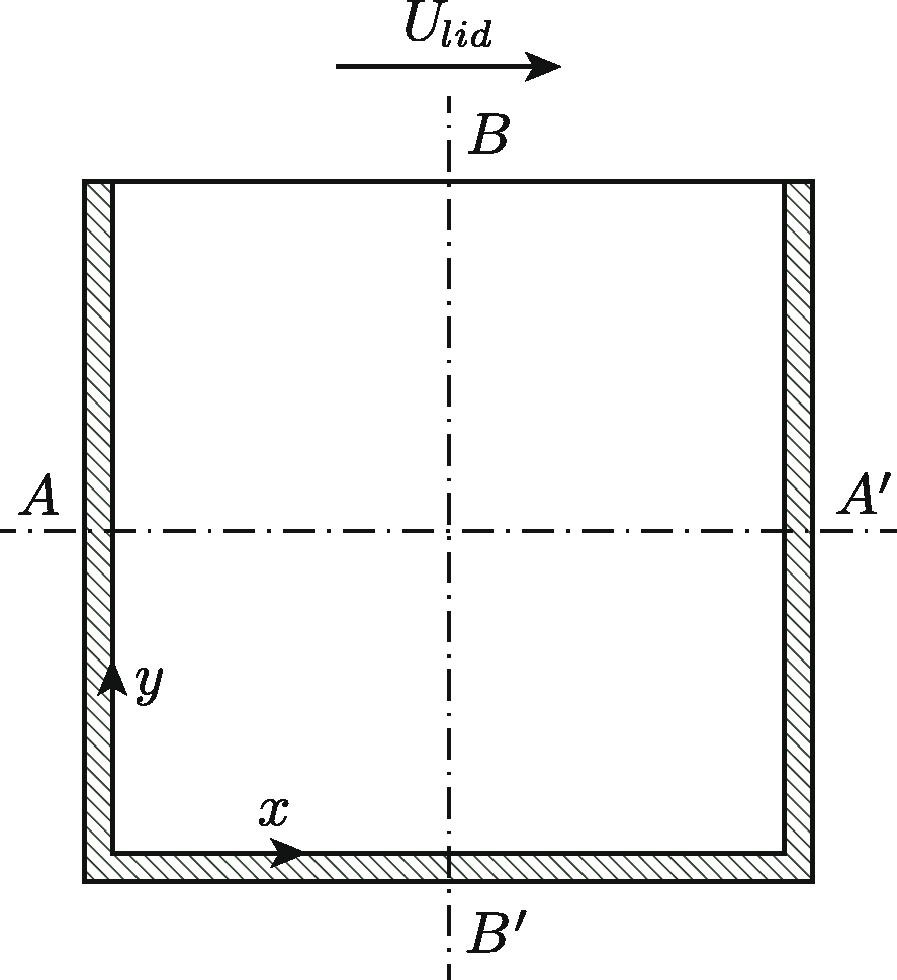
\includegraphics[width=.6\columnwidth]{cnrs-geometry}
	\caption{2m$\times$2m 2D domain of the CNRS Benchmark. $U_{lid}$
	represents the velocity along the top boundary. Various quantities are
	measured along the centerlines AA' and BB' for comparison. From Tiberga et
	al. \cite{tiberga_results_2020}.}
	\label{fig:cnrs-geometry}
\end{figure}

As shown in Figure \ref{fig:cnrs-geometry}, the domain geometry is a
2m$\times$2m square cavity filled with LiF-BeF$_2$-UF$_4$ molten salt at an
initial temperature of 900K \cite{tiberga_results_2020}.
Standard vacuum boundary conditions apply for neutron flux along all
boundaries whereby outgoing neutrons are considered lost, while homogeneous
boundary conditions apply for delayed neutron precursors. No-slip boundary
conditions apply for velocity variables in the cavity, except along the top
boundary for Steps 0.1, 0.3, 1.1, 1.2, and 1.4 which impose forced flow in the
form of lid-driven
cavity flow. For the temperature variable, all boundaries are insulated and we
simulate salt cooling with the following volumetric heat sink equation:
%
\begin{align}
    q'''(\vec{r}) &= \gamma \left(900 - T(\vec{r})\right) \label{eq:cnrs-heat}
    \shortintertext{where}
    q''' &= \mbox{volumetric heat sink [W$\cdot$m$^{-3}$],}
    \nonumber \\
    \gamma &= \mbox{heat transfer coefficient [W$\cdot$m$^{-3}\cdot$K$^{-1}$],}
    \nonumber \\
    T(\vec{r}) &= \mbox{temperature at point $\vec{r}$ [K].} \nonumber
\end{align}

Tiberga et al. \cite{tiberga_results_2020} used Serpent 2
\cite{leppanen_serpent_2014} with the JEFF-3.1 library
\cite{koning_jeff-31_2006} to generate multigroup neutronics data for the
LiF-BeF$_2$-UF$_4$ salt in the domain at 900K, which they condensed into six
energy groups and eight precursor groups. We direct readers to their paper for
the group constant data \cite{tiberga_results_2020}. In addition, the
benchmark prescribes the following equations to govern the temperature
dependence in the cross sections and the neutron diffusion coefficients:
%
\begin{align}
    \Sigma_i (T) &= \Sigma_i(T_{ref})
    \frac{\rho_{fuel}(T)}{\rho_{fuel}(T_{ref})}
    \shortintertext{and}
    D (T) &= D(T_{ref})
    \frac{\rho_{fuel}(T_{ref})}{\rho_{fuel}(T)}
    \shortintertext{where}
    \Sigma_i &= \mbox{relevant macroscopic cross section [cm${-1}$],}
    \nonumber \\
    D &= \mbox{neutron diffusion coefficient [cm$^2\cdot$s$^{-1}$],}   
    \nonumber \\
    \rho_{fuel} &= \mbox{density of the fuel salt [kg$\cdot$m$^{-3}$],}
    \nonumber \\
    T_{ref} &= \mbox{reference temperature} = 900\mbox{ K}. \nonumber
\end{align}

The benchmark also prescribes incompressible Navier-Stokes flow with the
Boussinesq approximation for evaluating the salt flow in the
domain, but does not restrict the type of neutronics model.
The following subsections briefly detail each benchmark step, with Table
\ref{table:benchmark} listing the relevant input parameters and observables.

\begin{table*}[tp!]
	\caption{Input parameters and observables of each benchmark step.}
	\centering
	\footnotesize
	\begin{tabular}{p{.05\textwidth} p{.4\textwidth} p{.6\textwidth}}
		\toprule
		\textbf{Step} & \textbf{Input parameters} & \textbf{Observables} \\
		\midrule
		0.1 &
		\begin{itemize}[nosep,noitemsep,left=0pt,
		                before={\begin{minipage}[t]{\hsize}},
                        after ={\end{minipage}}]
		    \item $U_{lid} = 0.5$ m$\cdot$s$^{-1}$
		\end{itemize}\vspace*{-\baselineskip}\mbox{} &
		\begin{itemize}[nosep,noitemsep,left=0pt,
		                before={\begin{minipage}[t]{\hsize}},
                        after ={\end{minipage}}]
		    \item Velocity components $(u_x,u_y)$ along AA' and BB'
		\end{itemize}\vspace*{-\baselineskip}\mbox{} \\
        \midrule
        0.2 &
        \begin{itemize}[nosep,noitemsep,left=0pt,
		                before={\begin{minipage}[t]{\hsize}},
                        after ={\end{minipage}}]
		    \item $U_{lid} = 0$ m$\cdot$s$^{-1}$
		    \item $T = 900$ K
		    \item $P = 1$ GW
		\end{itemize} &
		\begin{itemize}[nosep,noitemsep,left=0pt,
		                before={\begin{minipage}[t]{\hsize}},
                        after ={\end{minipage}}]
		    \item Fission rate density $\sum^6_g \Sigma_{f,g} \phi_g(\vec{r})$ along AA'
            \item Reactivity $\rho$
		\end{itemize}\vspace*{-\baselineskip}\mbox{} \\
        \midrule
        0.3 &
        \begin{itemize}[nosep,noitemsep,left=0pt,
		                before={\begin{minipage}[t]{\hsize}},
                        after ={\end{minipage}}]
		    \item Fixed flow field from Step 0.1 for
		    $U_{lid} = 0.5$ m$\cdot$s$^{-1}$
		    \item Fixed heat source distribution
		    $\sum^6_{g} \epsilon_g \Sigma_{f,g} \phi_g(\vec{r})$ from Step 0.2
		    \item $\gamma = 10^6$ W$\cdot$m$^{-3}\cdot$K$^{-1}$
		\end{itemize} &
		\begin{itemize}[nosep,noitemsep,left=0pt,
		                before={\begin{minipage}[t]{\hsize}},
                        after ={\end{minipage}}]
		    \item Temperature $T$ along AA' and BB'
		\end{itemize}\vspace*{-\baselineskip}\mbox{} \\
        \midrule
        1.1 &
        \begin{itemize}[nosep,noitemsep,left=0pt,
		                before={\begin{minipage}[t]{\hsize}},
                        after ={\end{minipage}}]
		    \item Fixed flow field from Step 0.1 for
		    $U_{lid} = 0.5$ m$\cdot$s$^{-1}$
		    \item $T = 900$ K
		    \item $P = 1$ GW
		\end{itemize} &
		\begin{itemize}[nosep,noitemsep,left=0pt,
		                before={\begin{minipage}[t]{\hsize}},
                        after ={\end{minipage}}]
		    \item Delayed neutron source $\sum^8_i \lambda_i C_i$ along AA' and BB'
		    \item Reactivity change between Step 1.1 and Step 0.2,
		    $\Delta \rho = \rho - \rho_{s_{0.2}}$
		\end{itemize}\vspace*{-\baselineskip}\mbox{} \\
        \midrule
        1.2 &
        \begin{itemize}[nosep,noitemsep,left=0pt,
		                before={\begin{minipage}[t]{\hsize}},
                        after ={\end{minipage}}]
		    \item Fixed flow field from Step 0.1 for
		    $U_{lid} = 0.5$ m$\cdot$s$^{-1}$
		    \item $P = 1$ GW
		    \item $\gamma = 10^6$ W$\cdot$m$^{-3}\cdot$K$^{-1}$
		\end{itemize}\vspace*{-\baselineskip}\mbox{} &
		\begin{itemize}[nosep,noitemsep,left=0pt,
		                before={\begin{minipage}[t]{\hsize}},
                        after ={\end{minipage}}]
		    \item Temperature $T$ along AA' and BB'
            \item Reactivity change between Step 1.2 and Step 1.1,
            $\Delta\rho = \rho - \rho_{s_{1.1}}$
            \item Change in fission rate density
            $\sum^6_g \Sigma_{f,g} \phi_g(\vec{r}) -
            \left[\sum^6_g \Sigma_{f,g} \phi_g(\vec{r})\right]_{s_{0.2}}$
		\end{itemize} \\
        \midrule
        1.3 &
        \begin{itemize}[nosep,noitemsep,left=0pt,
		                before={\begin{minipage}[t]{\hsize}},
                        after ={\end{minipage}}]
		    \item $P = 1$ GW
		    \item $U_{lid} = 0$ m$\cdot$s$^{-1}$
		    \item $\gamma = 10^6$ W$\cdot$m$^{-3}\cdot$K$^{-1}$
		\end{itemize}\vspace*{-\baselineskip}\mbox{} &
		\begin{itemize}[nosep,noitemsep,left=0pt,
		                before={\begin{minipage}[t]{\hsize}},
                        after ={\end{minipage}}]
		    \item Velocity components $(u_x, u_y)$ along AA' and BB'
            \item Temperature $T$ along AA' and BB'
            \item Delayed neutron source $\sum^8_i \lambda_i C_i$ along AA' and BB'
            \item Reactivity change from Step 0.2
        $\Delta\rho = \rho - \rho_{s_{0.2}}$
		\end{itemize} \\
        \midrule
        1.4 &
        \begin{itemize}[nosep,noitemsep,left=0pt,
		                before={\begin{minipage}[t]{\hsize}},
                        after ={\end{minipage}}]
		    \item $\gamma = 10^6$ W$\cdot$m$^{-3}\cdot$K$^{-1}$
		    \item $P$ variable in the range $[0,1]$ GW with a step of 0.2 GW
		    \item $U_{lid}$ variable in the range $[0,0.5]$ m$\cdot$s$^{-1}$
		    with a step of 0.1 m$\cdot$s$^{-1}$
		\end{itemize} &
		\begin{itemize}[nosep,noitemsep,left=0pt,
		                before={\begin{minipage}[t]{\hsize}},
                        after ={\end{minipage}}]
		    \item Reactivity change between Step 1.4 and Step 0.2,
		    $\Delta\rho = \rho - \rho_{s_{0.2}}$, for all permutations of $P$
		    and $U_{lid}$ values
		\end{itemize}\vspace*{-\baselineskip}\mbox{} \\
        \midrule
        2.1 &
        \begin{itemize}[nosep,noitemsep,left=0pt,
		                before={\begin{minipage}[t]{\hsize}},
                        after ={\end{minipage}}]
		    \item $\gamma = 10^6$ W$\cdot$m$^{-3}\cdot$K$^{-1}$
            \item Steady-state solution from Step 1.4 for $U_{lid} = 0.5$
        m$\cdot$s$^{-1}$ and $P = 1.0$ GW
		\end{itemize} &
		\begin{itemize}[nosep,noitemsep,left=0pt,
		                before={\begin{minipage}[t]{\hsize}},
                        after ={\end{minipage}}]
		    \item Power gain and shift as a function of the perturbation frequency
		\end{itemize}\vspace*{-\baselineskip}\mbox{} \\
		\bottomrule
	\end{tabular}
	\label{table:benchmark}
\end{table*}

\subsection{Phase 0: Single physics}

In this preliminary phase, the steady-state solutions of
individual physics are studied without any multiphysics coupling.

\subsubsection{Step 0.1: Velocity field}

This step investigates the steady-state incompressible flow distribution in the
domain from a lid-driven cavity flow by imposing a non-zero horizontal
velocity along the top boundary. In addition, this step provides a fixed
velocity field for Steps 0.3, 1.1, and 1.2.

\subsubsection{Step 0.2: Neutronics}

This step tests neutronics capabilities through a criticality eigenvalue
problem in a static, isothermal fuel configuration by solving for the fission
rate density and effective multiplication factor $k_{eff}$. This step also aims
to identify deviations in results attributable to differences in neutronics
models and approximations. The total power $P$ is fixed to normalize the
neutron fluxes. For neutronics models conforming to the six neutron energy
group structure provided by Tiberga et al. \cite{tiberga_results_2020},
fission rate density is calculated as:
%
\begin{align}
    \text{Fission rate density} =& \sum^6_g \Sigma_{f,g} \phi_g(\vec{r})
    \shortintertext{where}
    \Sigma_{f,g} =& \text{ macroscopic fission cross section for neutron}
    \nonumber \\
    &\text{ in group $g$,} \nonumber \\
    \phi_g =& \text{ neutron flux in group $g$.} \nonumber
\end{align}

\subsubsection{Step 0.3: Temperature}

This step assesses passive scalar transport capability for determining the
temperature distribution independently from
the fluid flow and neutronics problems by imposing fixed velocity and fission
heat source distributions from Steps 0.1 and 0.2, respectively. Similar to the
fission rate density, the heat source distribution in six-group neutronics
models is calculated as:
%
\begin{align}
    \text{Heat source distribution} =& \sum^6_{g} \epsilon_g \Sigma_{f,g}
    \phi_g(\vec{r})
    \shortintertext{where}
    \epsilon_g =& \text{ average fission energy released by neutrons}
    \nonumber \\
    &\text{ in group $g$.} \nonumber
\end{align}

\subsection{Phase 1: Steady-state coupling}

Phase 1 builds towards simulating a fully-coupled multiphysics steady-state
system by gradually introducing coupling between various physics present in
a fast-spectrum molten salt system. All simulations are solved as steady-state
criticality eigenvalue problems.

\subsubsection{Step 1.1: Circulating fuel}

This step investigates effects of fuel salt flow on the neutronics,
namely the reactivity loss from the movement of precursors. The delayed neutron
precursors are allowed to drift under the fixed velocity field from Step 0.1
while keeping the temperature $T$ fixed at 900 K. With eight precursor groups,
the delayed neutron source is calculated as:
%
\begin{align}
    \text{Delayed neutron source} =& \sum^8_i \lambda_i C_i
    \shortintertext{where}
    \lambda_i =& \text{ average decay constant of delayed neutron} \nonumber \\
    &\text{ precursors in precursor group $i$,} \nonumber \\
    C_i =& \text{ concentration of delayed neutron precursors in}
    \nonumber \\
    &\text{ precursor group $i$.} \nonumber
\end{align}

\subsubsection{Step 1.2: Power coupling}

This step assesses the capability to accurately reproduce the change in
neutron flux distribution due to the fuel density reactivity feedback between
the neutron fluxes and the temperature distribution. We solve for the
steady-state neutron flux and temperature distributions under the fixed
velocity field from Step 0.1 and a volumetric heat sink described by Equation
\ref{eq:cnrs-heat}.

\subsubsection{Step 1.3: Buoyancy}

Building on the previous step, we replace the fixed velocity field with
buoyancy-driven flow arising from the temperature gradients for a fully-coupled
multiphysics problem without forced flow. Barring any major discrepancies in
the previous steps, this step assesses the capability to reproduce the correct
buoyancy-driven flow profile and the subsequent effects on the neutronics and
temperature distribution due to precursor drift and fuel density reactivity
feedback.

\subsubsection{Step 1.4: Full coupling}

This step introduces forced flow to the fully-coupled problem through the
non-zero $U_{lid}$ boundary
condition. Thus, this problem most closely represents a molten salt system with
1) flow driven by an external force, 2) buoyancy flow effects, 3) \gls{DNP}
drift, and 4) thermal feedback effects on the neutronics. We solve for the
$k_{eff}$ under a range of $U_{lid}$ and $P$ values given in Table
\ref{table:benchmark}.

\subsection{Phase 2: Time dependent coupling}

In this phase, the transient response of the fully coupled nonlinear system is
studied.

\subsubsection{Step 2.1: Forced convection transient}

Linear perturbation analyses are performed in this step by introducing periodic
perturbations to the heat transfer coefficient $\gamma$ and studying the gain
and phase shift of the response in the total power $P$. For the initial
conditions, the steady-state solution from Step 1.4 with
$U_{lid} = 0.5$ m$\cdot$s$^{-1}$ and $P = 1$ GW is used. This initial
configuration is made exactly critical by scaling the neutron source terms,
from fission and \gls{DNP} decay, by the inverse of the criticality eigenvalue
solution from Step 1.4.

$\gamma$ is uniformly perturbed according to small-amplitude sine waves given
as:
%
\begin{align}
    \gamma =& \gamma_0 \left[ 1 + 0.1\sin\left(2 \pi f \right) \right]
    \shortintertext{where}
    \gamma_0 =& 10^6 \mbox{ W$\cdot$m$^{-3}\cdot$K$^{-1}$}, \nonumber \\
    f \in& \left\lbrace 0.0125, 0.025, 0.05, 0.1, 0.2, 0.4, 0.8 \right\rbrace 
    \mbox{ Hz.} \nonumber
\end{align}

The benchmark defines power gain as:
%
\begin{align}
    \mbox{Power gain} =& \frac{\left(P_{max} - P_{avg}\right)/P_{avg}}{
    \left(\gamma_{max} - \gamma_{avg}\right)/\gamma_{avg}}
\end{align}
%
The subscripts denote the maximum and time-averaged values of $P$ and $\gamma$.

\FloatBarrier

\section{Modeling Approach with Moltres} \label{sec:model}

This section describes the specific modeling approach for
simulating the CNRS Benchmark cases in Moltres.

For this work\footnote{The input files for
all benchmark
cases are available on the Moltres GitHub repository at 
\url{https://github.com/arfc/moltres/tree/devel/problems/2021-cnrs-benchmark}.
}, I ran the benchmark cases on a uniformly-spaced mesh
of 200$\times$200 elements. Thus, the dimensions of each mesh element are
0.01m$\times$0.01m. I adopted the group constant data
provided by Tiberga et al. \cite{tiberga_results_2020}. Next, I
discretized most variables, i.e., neutron fluxes, velocity
components, pressure, and temperature, using continuous, first-order, Lagrange
shape functions. The only exception is the precursor concentration variables,
which I discretized using zeroth-order monomial shape functions and solved
using a \gls{DFEM}. I interpolated the resulting discontinuous,
cell-centered precursor values to obtain the nodal values for results
analysis.

The
\texttt{Navier-Stokes} and \texttt{Heat} \texttt{Conduction} modules from
\gls{MOOSE} provide some of the capabilities for
modeling incompressible flow and heat transfer. In particular, I stabilized
the incompressible flow and temperature governing equations using the
\gls{SUPG} stabilization method implemented in \gls{MOOSE}
\cite{peterson_overview_2018}. Without \gls{SUPG} stabilization, I
observed spurious numerical oscillations in the velocity and temperature near
the top boundary due to the singularity on the top left corner where different
velocity boundary conditions meet. I also applied the \gls{PSPG} stabilization
scheme \cite{hughes_new_1986} from the Navier-Stokes module
\cite{peterson_overview_2018},
which enables equal-order discretizations in the velocity and pressure
variables. Equal-order discretizations with \gls{PSPG} are computationally
cheaper and more convenient than implementing higher-order
velocity discretizations for stability without \gls{PSPG}
\cite{chapelle_inf-sup_1993}.

Using the inverse power method solver in \gls{MOOSE}, I ran all eigenvalue calculations in
Steps 0.2, 1.1, 1.2, 1.3, and 1.4. I ran all other steps
using the Preconditioned Newton-Krylov solver
\cite{gaston_physics-based_2015}. The coupled steady-state problems in
Steps 1.2, 1.3, and 1.4 required segregated solvers for the neutronics
and the thermal-hydraulics due to the unique problem setups involving a
criticality search problem for the neutron multiplication factor
and a steady-state problem in thermal-hydraulics simultaneously.

\begin{table}[tb]
    \caption{Timestep sizes used for the time-dependent cases in
    Step 2.1, corresponding to 1/200th of the perturbation period.}
	\centering
	\setlength\tabcolsep{2.5pt}
	\begin{tabular}{l l l l l l l l}
	    \toprule
	    Frequency [Hz] & 0.0125 & 0.025 & 0.05 & 0.1 & 0.2 & 0.4 & 0.8 \\
	    \midrule
	    Timestep size [s] & 0.2 & 0.2 & 0.1 & 0.05 & 0.025 & 0.0125 & 0.00625
	    \\
	    \bottomrule
	\end{tabular}
	\label{table:timestep}
\end{table}

For the time-dependent cases in Step 2.1, I employed full coupling with
a second-order implicit Backward Differential Formula (BDF2) time-stepping
scheme. I set the timestep sizes for each driving frequency in the heat transfer
coefficient to 1/200th of the perturbation period. Table
\ref{table:timestep} shows the timestep sizes. I assumed the
systems reached asymptotic behavior when the magnitudes of neighboring power
peaks differed by less than 0.001\% for at least ten wavelengths. Under this
assumption, the phase shift measurements between adjacent waves always
converged before the magnitude measurements of the power peaks.

Table \ref{table:software} compares the numerical methods, meshing schemes, and
neutronics models of Moltres and the four participating software packages in
the CNRS benchmark paper \cite{tiberga_results_2020}. The $SP_N$ and
$S_N$ neutronics models refer to the simplified $P_N$ spherical harmonics and
$S_N$ discrete ordinates neutron transport models, respectively. Based on the
solvers and methods of solution, Moltres is most similar to the
PHANTOM-$S_N$ + DGFlows \cite{tiberga_discontinuous_2019} multiphysics package
from \gls{TUD} with the $S_2$ neutron transport model. Participants from
\gls{CNRS} and \gls{PSI}
employed non-uniform meshes which were refined near the boundaries. In contrast,
we and the \gls{PoliMi} and \gls{TUD} participants employed uniform meshes.

\FloatBarrier

\begin{landscape}
\begin{table*}[p]
    \caption{List of software packages and their corresponding model
    specifications for the CNRS Benchmark simulations
    \cite{tiberga_results_2020}.}
    \centering
    \begin{tabular}{p{4.2cm} p{7cm} p{3.3cm} p{2cm} p{2.7cm}}
        \toprule
        Software & Institute & Numerical method & Mesh & Neutronics model \\
        \midrule
        OpenFOAM & Centre national de la recherche scientifique (CNRS) & Finite volume & 200$\times$200 \newline Non-uniform & $SP_1$ \& $SP_3$ \\
        OpenFOAM & Politecnico di Milano (PoliMi) & Finite volume & 400$\times$400 \newline Uniform & Neutron diffusion \\
        GeN-Foam & Paul Scherrer Institute (PSI) & Finite volume & 200$\times$200 \newline Non-uniform & Neutron diffusion \\
        PHANTOM-$S_N$+DGFlows & Delft University of Technology (TUD) & Discontinuous finite \newline element & 50$\times$50 \newline Uniform & $S_2$ \& $S_6$ \\
        Moltres (This work) & University of Illinois at Urbana-Champaign (UIUC) & Continuous \& discontinuous finite element & 200$\times$200 \newline Uniform & Neutron diffusion \\
        \bottomrule
    \end{tabular}
    \label{table:software}
\end{table*}
\end{landscape}

\FloatBarrier

\section{Results}

In this section, we compare the results from Moltres for each CNRS Benchmark
step to the results in the benchmark paper \cite{tiberga_results_2020}.
The software packages from \gls{CNRS} and \gls{TUD}
each report two sets of results arising from different angular discretizations
in their neutronics models for Steps 0.2, 1.1, 1.2, 1.3, 1.4, and 2.1. These
sets of results are labeled as CNRS-$SP_1$ and
CNRS-$SP_3$; and TUD-$S_2$ and TUD-$S_6$, respectively. The
authors performed code-to-code verification by sampling observable values at
201 equidistant points along the centerlines AA' and BB' and reporting the
discrepancy $\epsilon_c$ of each observable from each software
(indexed by $c$) for each measured observable $Q_c$ (not to be confused with
fission heat source $Q_f$), relative to the average of
that same observable $Q_{avg}$ from all participating software. Variables
$\epsilon_c$ and $Q_{avg}$ are calculated as:
%
\begin{align}
    \epsilon_c =& \sqrt{\frac{\sum^{N_p}_{i=1}\left[Q_c(\vec{r_i}) - Q_{avg}
    (\vec{r_i})\right]^2}{\sum^{N_p}_{i=1} Q^2_{avg}(\vec{r_i})}}
    \shortintertext{and}
    Q_{avg}(\vec{r_i}) =& \frac{1}{N_c} \sum^{N_c}_{c=1} Q_c(\vec{r_i})
    \shortintertext{where}
    Q_c(\vec{r_i}) =&
    \mbox{ value of observable $Q$ at location $\vec{r_i}$ from software $c$,}
    \nonumber \\
    N_p =& \mbox{ number of sampling points of quantity $Q$} = 201,
    \nonumber \\
    N_c =& \mbox{ number of participating software packages.} \nonumber
\end{align}

The average discrepancy $\epsilon$ over all software is calculated as:
%
\begin{align}
    \epsilon =& \frac{1}{N_c}\sum^{N_c}_{c=1} \epsilon_c
\end{align}

We adopted the averaged values $\epsilon$ and $Q_{avg}$ directly from the
reference work \cite{tiberga_results_2020} without including our results
in the calculations. We note that the benchmark does not provide a reference
solution and a significantly erroneous value from one of the software packages
could heavily skew the discrepancy values. Nevertheless, the benchmark paper
reports good agreement among their software packages.

For observables measured along the centerlines AA' and/or BB', Tables
\ref{table:disc0} and \ref{table:disc1} report the discrepancy $\epsilon_c$ of
each observable from Moltres relative to the average of the benchmark
participants $Q_{avg}$ alongside the average discrepancy $\epsilon$ of
the benchmark participants. We also reproduce corresponding plots
in the benchmark paper for every observable along AA' or BB' in Figures
\ref{fig:0.1}, \ref{fig:0.2}, \ref{fig:0.3}, \ref{fig:1.1}, \ref{fig:1.2},
\ref{fig:1.3}, and \ref{fig:2.1} for a qualitative comparison of the results
from Moltres and the benchmark participants. Given the significant overlap in
the plot curves, these figures omit results from CNRS-$SP_1$ and TUD-$S_2$ to
reduce cluttering. Readers may also refer to
\ref{appendix:tables} for tables of observable values at nine equidistant
points along AA' and BB' from Moltres and the benchmark participants. We
provide these tables for ease of review and a direct comparison to
corresponding data tables from \cite{tiberga_results_2020}. The full dataset
of all observable results used in this results analysis is
available at \cite{park_results_2021}. Lastly, Table
\ref{table:rho} reports all reactivity and change in reactivity results from
Steps 0.2, 1.1, 1.2, and 1.3.

\begin{figure}[h]
	\centering
    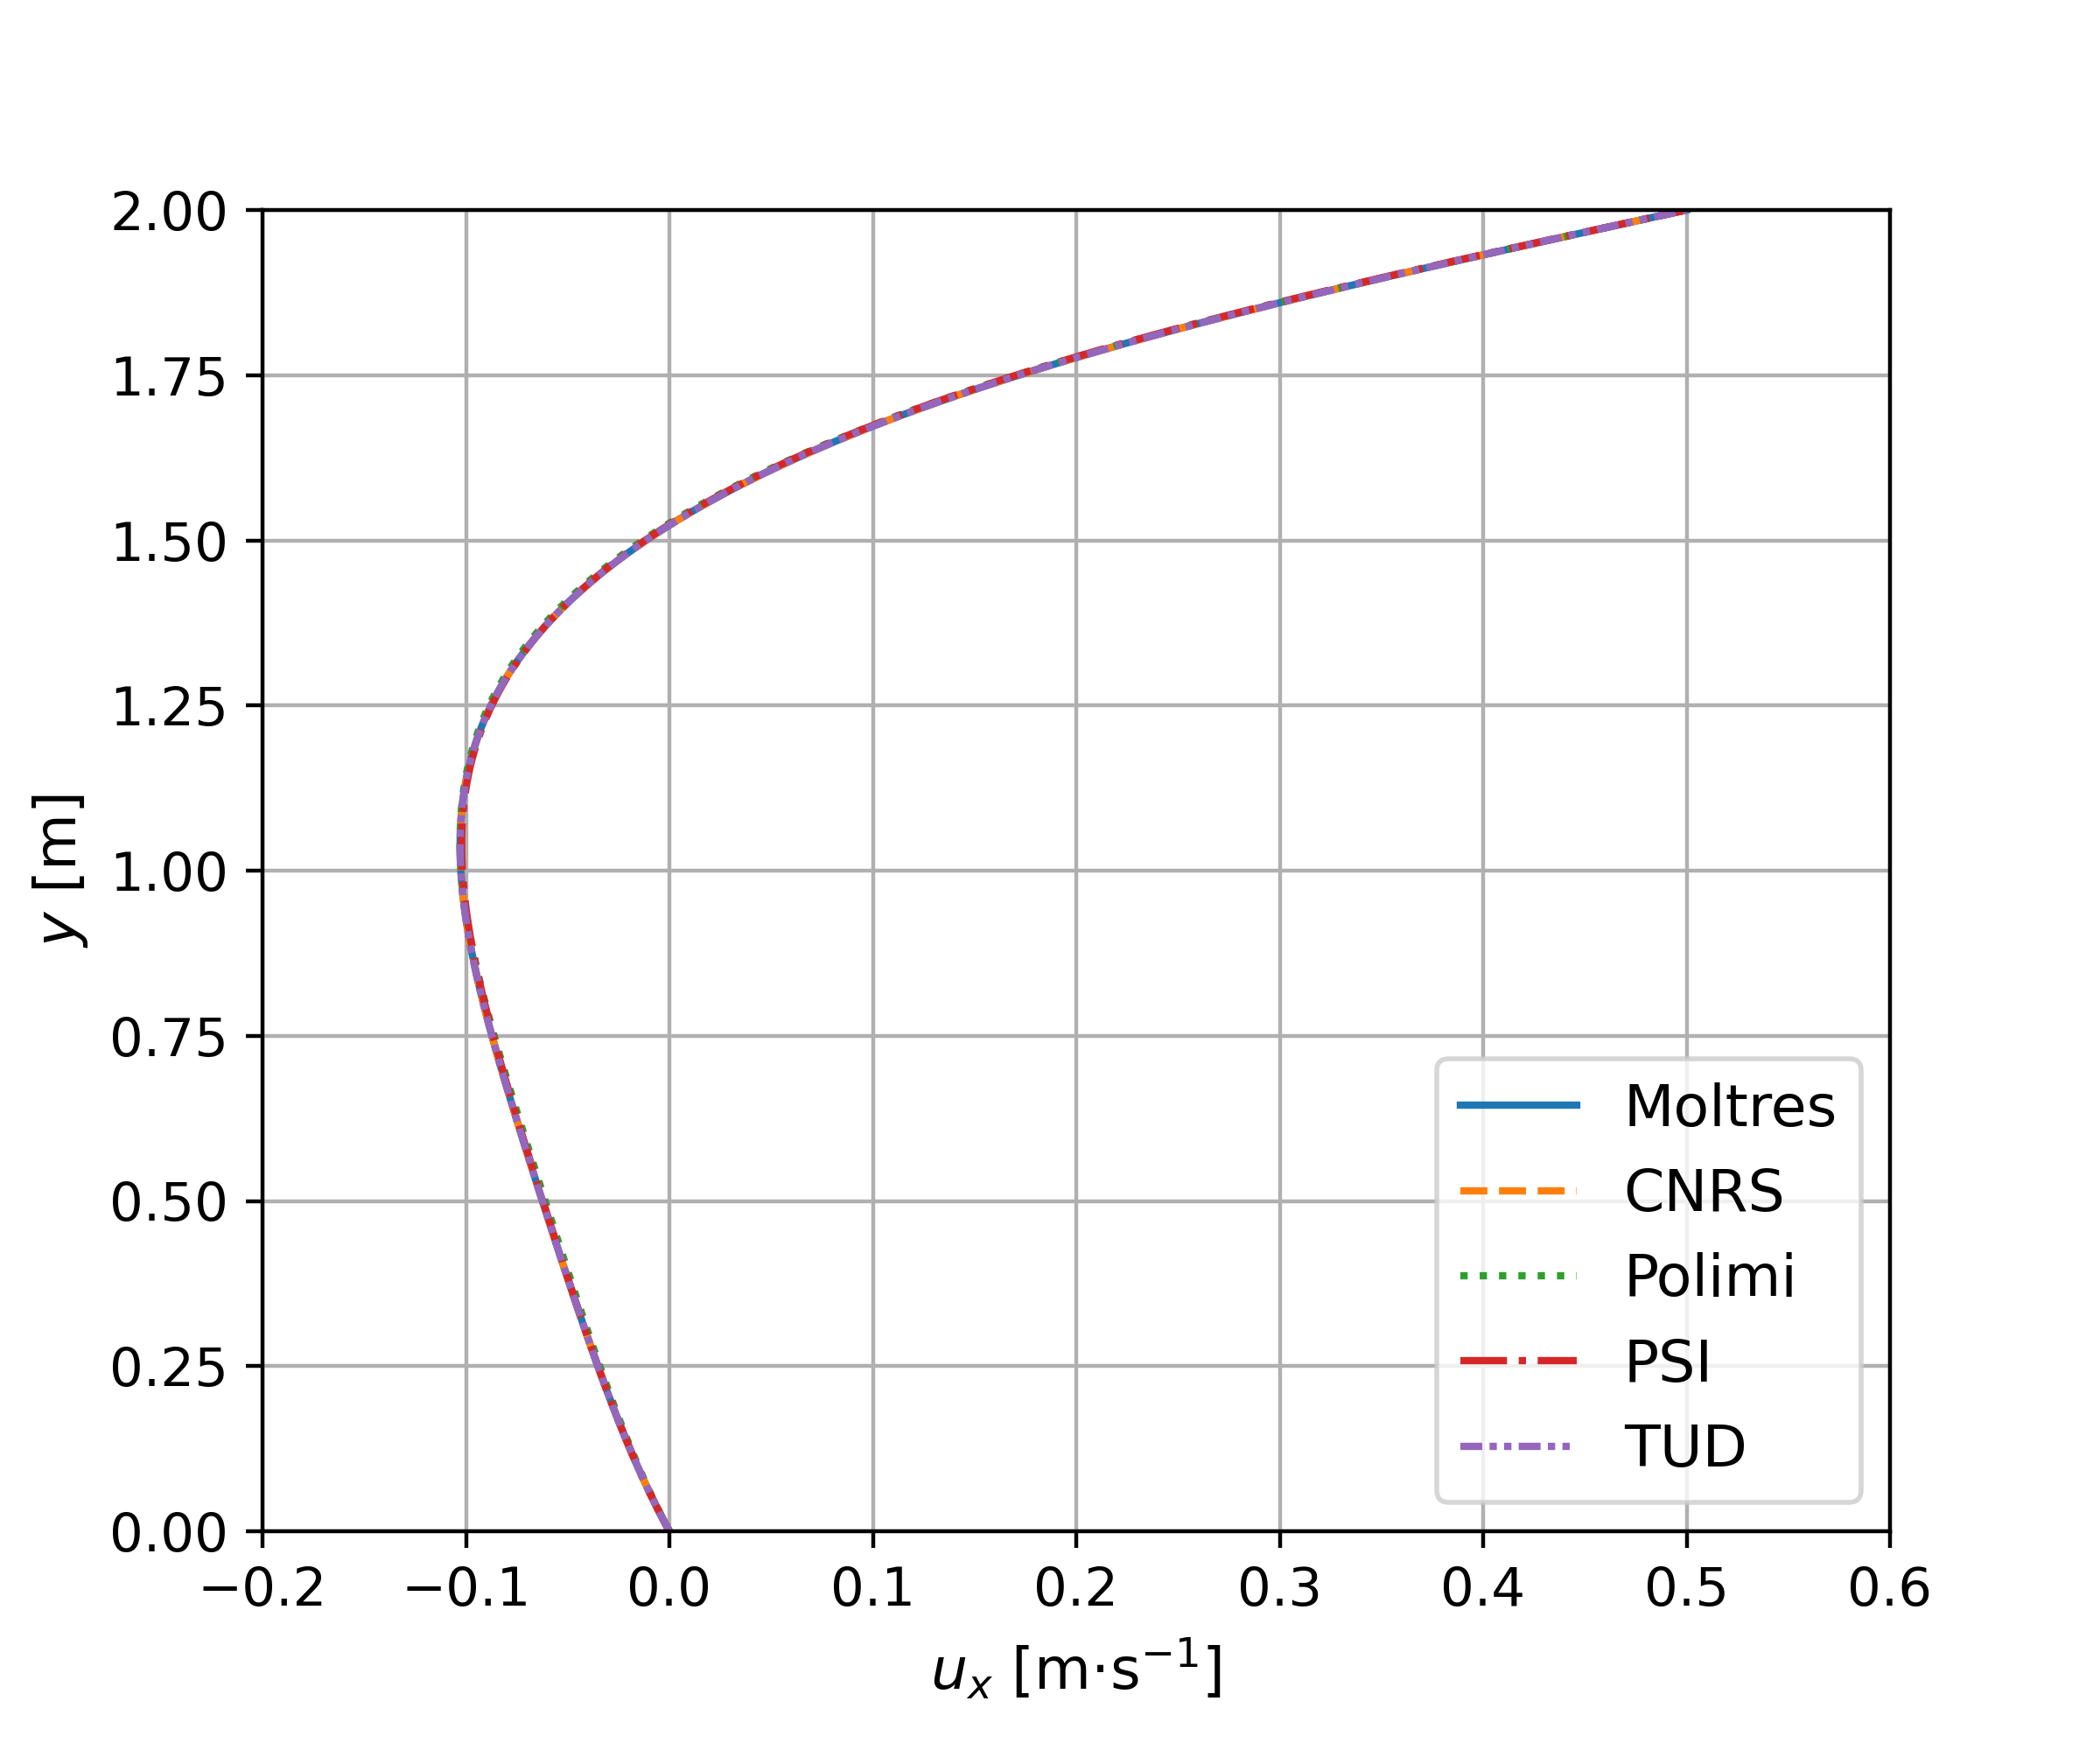
\includegraphics[width=.75\columnwidth]{0-1-vel-plot}
	\caption{Step 0.1 \textemdash\ Horizontal velocity component along BB'.}
	\label{fig:0.1}
\end{figure}
%
\begin{figure}[h]
	\centering
	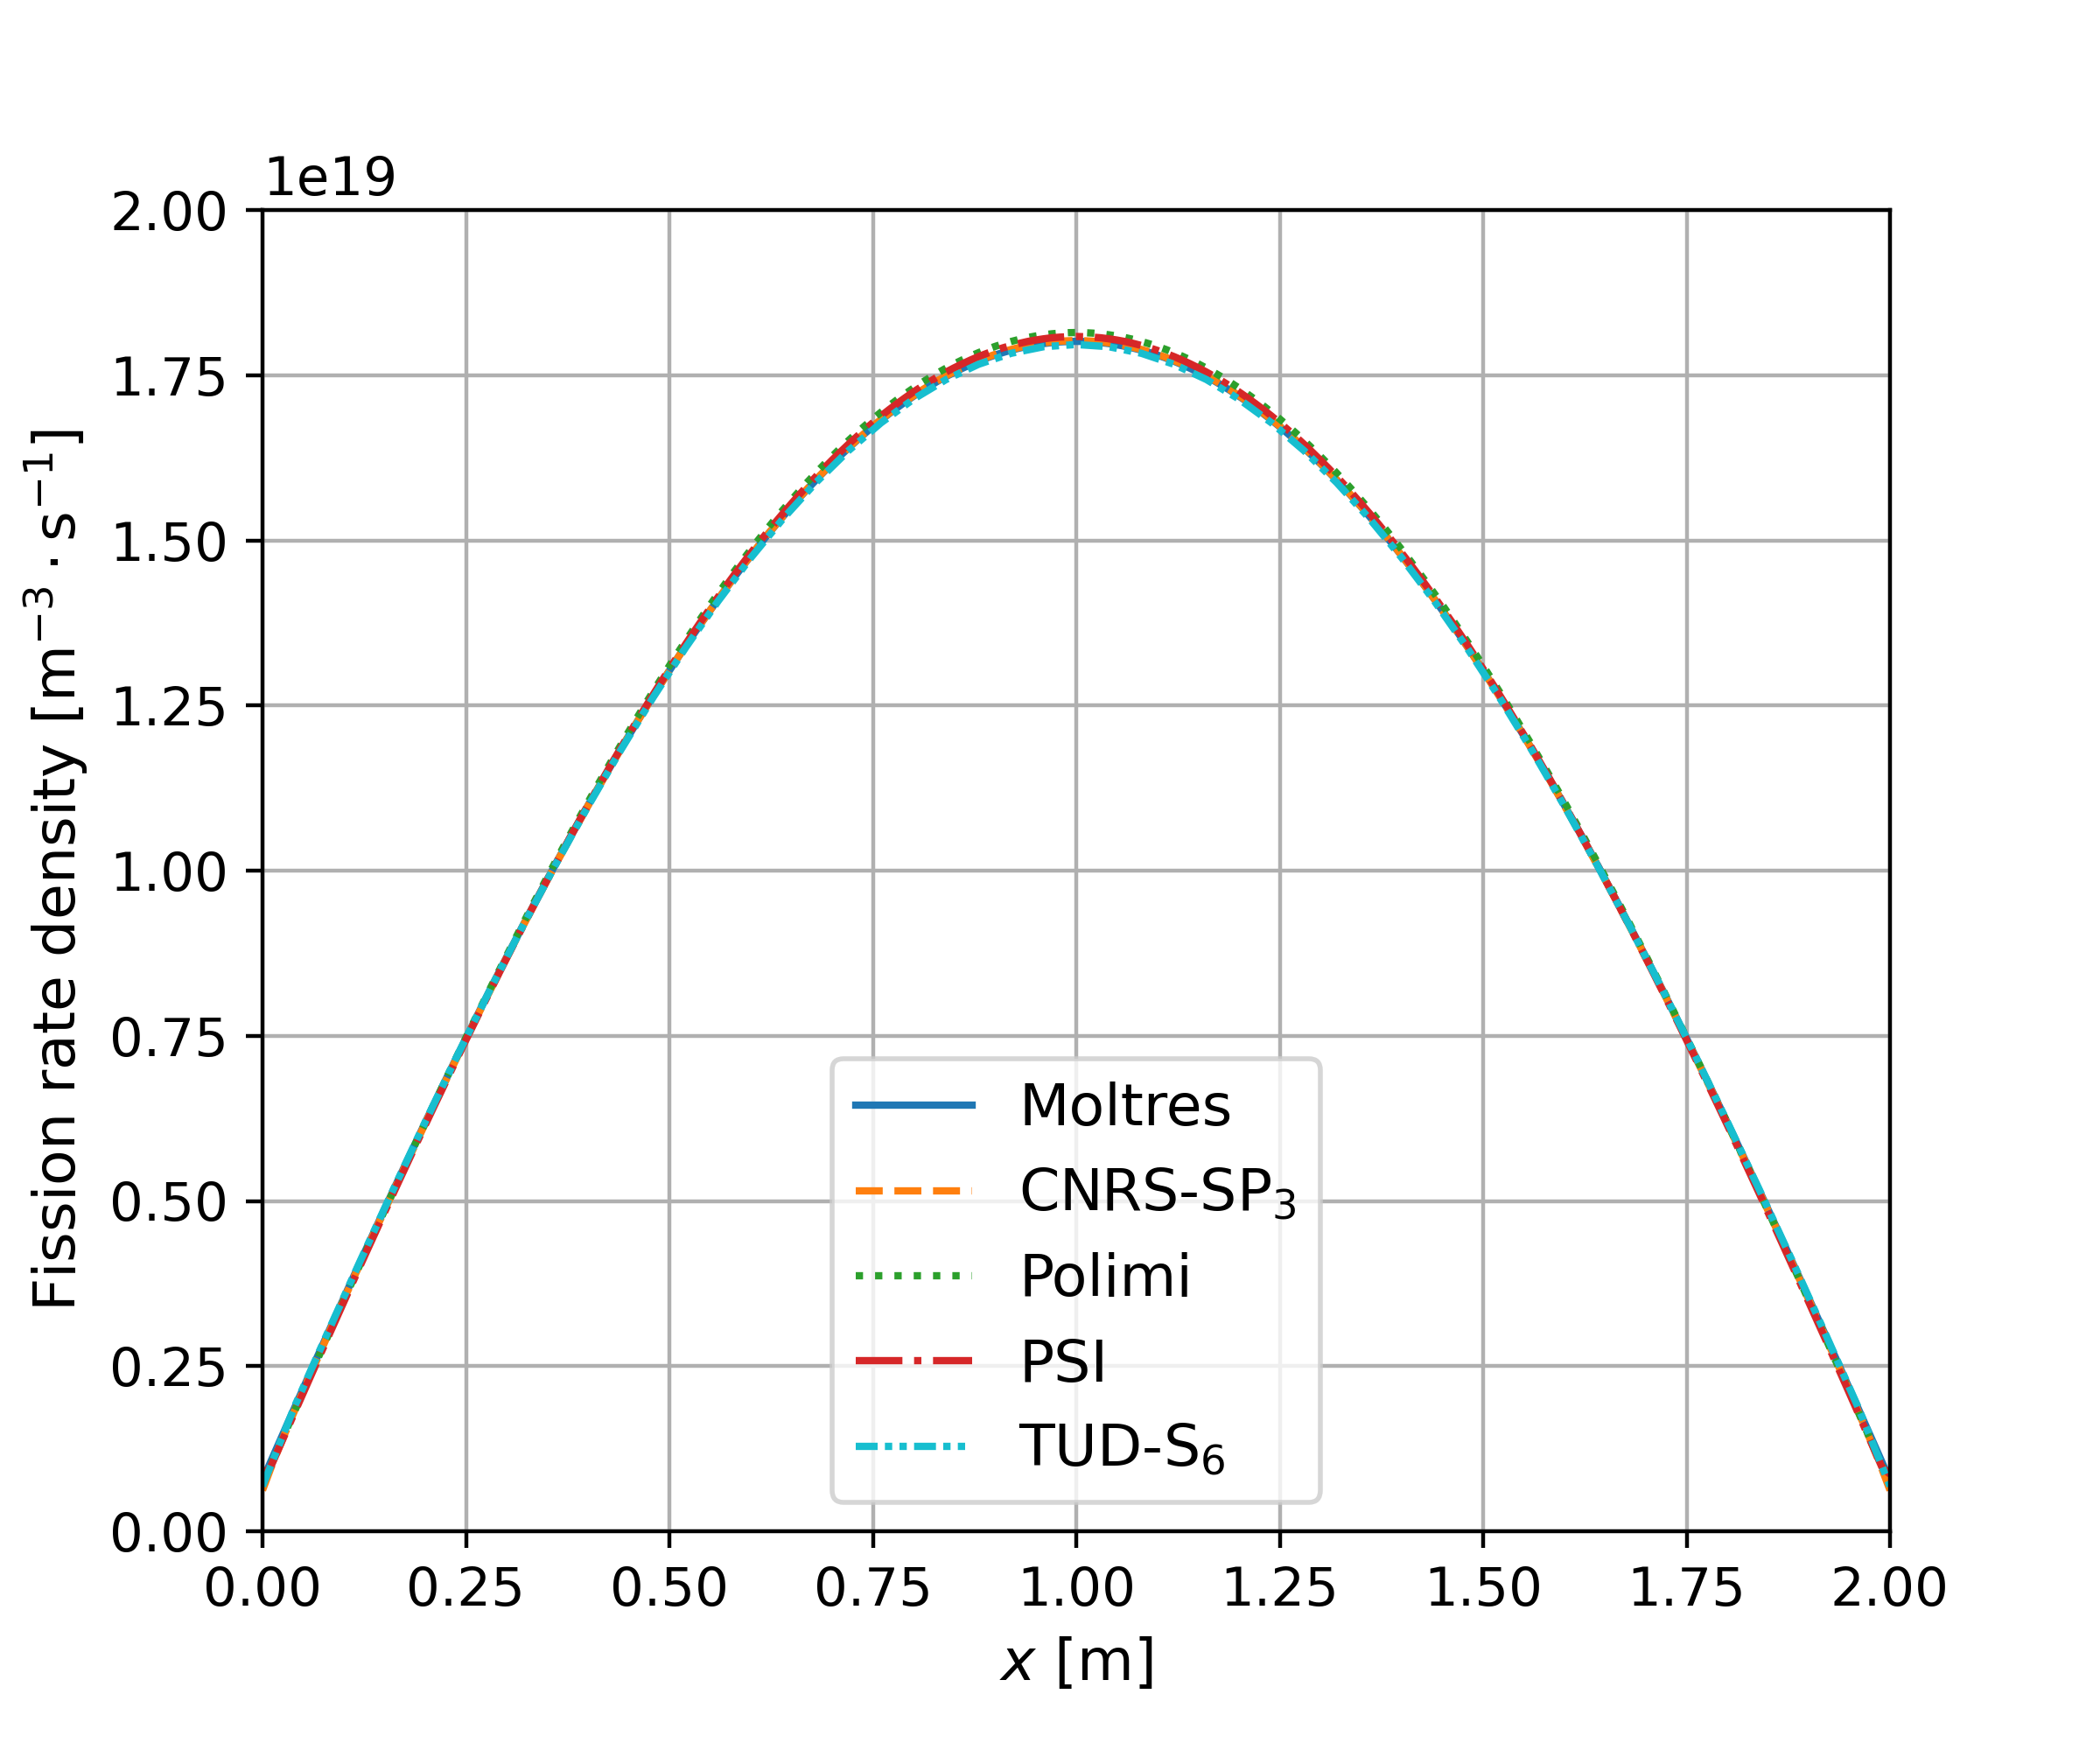
\includegraphics[width=.75\columnwidth]{0-2-fiss-plot}
	\caption{Step 0.2 \textemdash\ Fission rate density along AA'.}
	\label{fig:0.2}
	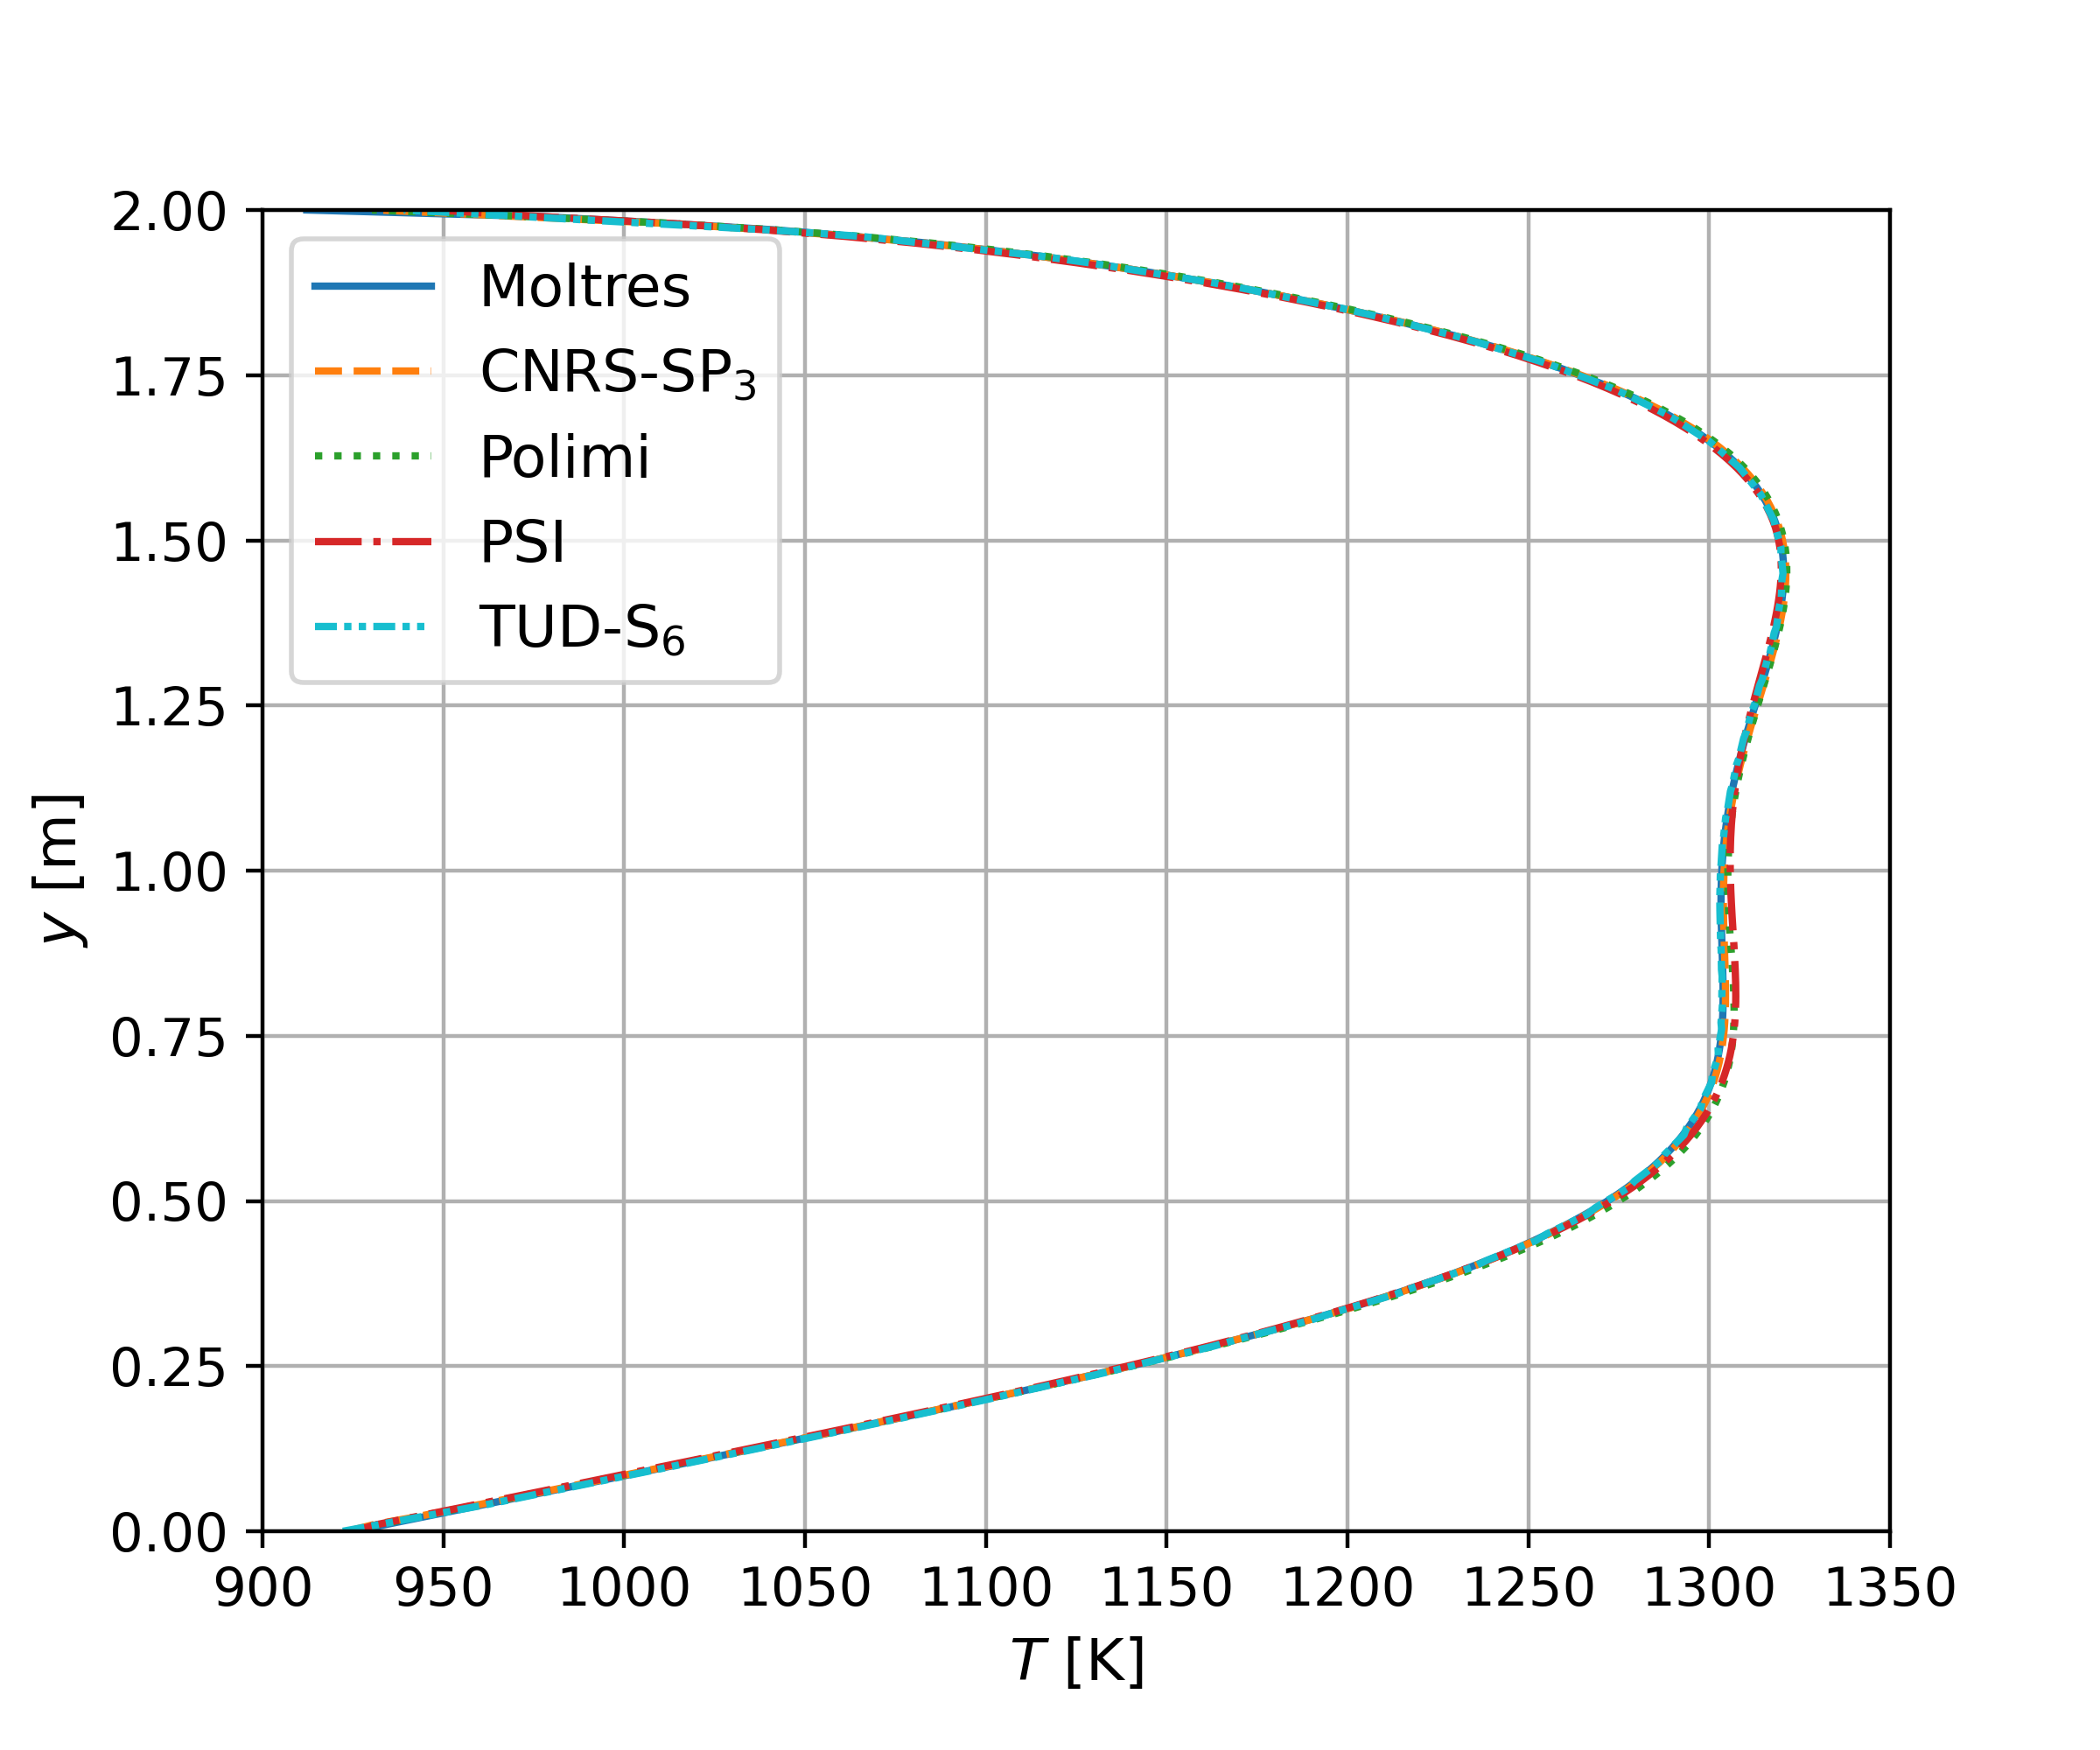
\includegraphics[width=.75\columnwidth]{0-3-temp-plot}
	\caption{Step 0.3 \textemdash\ Temperature distribution along BB'.}
	\label{fig:0.3}
\end{figure}
%
\FloatBarrier
%
\begin{table}[htb]
	\caption{Discrepancy values from Moltres alongside the average and standard
	deviation of the discrepancy values of the benchmark participants for Phase
	0.}
	\centering
	\small
	\begin{tabular}{l l c S S S}
		\toprule
		\multirow{2}{*}{\textbf{Step}} & \multirow{2}{*}{\textbf{Observable}} & \multirow{2}{*}{\textbf{Centerline}} & {\multirow{2}{*}{\textbf{Moltres [\%]}}} & \multicolumn{2}{c}{\textbf{Benchmark [\%]}} \\
		& & & & {Average} & {SD} \\
		\midrule
		\multirow{4}{*}{0.1} &
		\multirow{2}{*}{$u_x$} & AA' & 0.247 & 0.253 & 0.150 \\
		& & BB' & 0.266 & 0.318 & 0.102 \\
		\cmidrule{2-6}
		& \multirow{2}{*}{$u_y$} & AA' & 0.540 & 0.598 & 0.266 \\
		& & BB' & 0.468 & 0.795 & 0.421 \\
		\midrule
		{0.2} &
		{$\sum^6_g \Sigma_{f,g} \phi_g(\vec{r})$} & AA' & 0.313 & 0.285 & 0.153
		\\
		\midrule
		\multirow{2}{*}{0.3} &
		\multirow{2}{*}{$T$} & AA' & 0.090 & 0.085 & 0.031 \\
		& & BB' & 0.164 & 0.083 & 0.027\\
		\bottomrule
	\end{tabular}
	\label{table:disc0}
\end{table}

\subsection{Phase 0 results \& discussion}

Figures \ref{fig:0.1}, \ref{fig:0.2}, and \ref{fig:0.3} show that Moltres
accurately reproduced all three sets of results in Phase 0 for the velocity
field, fission rate density, and temperature. Table
\ref{table:disc0} reports the discrepancy values from Moltres for Phase 0 and
the corresponding average and \gls{SD} of the discrepancy values from
the benchmark participants
\cite{tiberga_results_2020}. Moltres performs very well as most discrepancy
values are either lower than or fall within one \gls{SD} of the benchmark
average discrepancies. The discrepancy value for $T$ along centerline BB' in
Step 0.3 is the only exception with its value of 0.164\% being larger than
the benchmark average by 3 \gls{SD}.

We
note in Figure \ref{fig:0.3} that the $T$ distribution from Moltres is almost
identical to the corresponding distributions from CNRS-$SP_3$ and TUD-$S_6$
along most of centerline BB'. However, Figure \ref{fig:0.3-zoom} shows
significant spread in the $T$ distributions along BB' from all software
packages near the top boundary. At $y = 2.0$ m, Moltres underpredicts the
temperature at 912.3 K compared to the benchmark participants' values which
range between 930.3 K and 948.1 K (Refer to Table \ref{table:0.3} for the
numerical values). This point on the top boundary lies directly downstream of
the velocity boundary condition discontinuity at the top-left corner.
Corner singularities are generally difficult to approximate with
continuous Galerkin methods \cite{kuhlmann_lid-driven_2018}.
The \gls{SUPG} stabilization scheme dampens numerical oscillations by
introducing pointwise artificial thermal diffusivity which depends strongly on
the inverse of local velocity magnitude \cite{peterson_overview_2018}.
Therefore, while the \gls{SUPG} scheme was very effective in eliminating
spurious numerical oscillations everywhere else, it provides little damping
along the top boundary due to the relatively large non-zero velocity boundary
condition. On the other hand, the temperature values in the rest of the domain
and the average discrepancies of the other variables show that Moltres can
still accurately reproduce the expected results and the temperature deviations
along the top boundary do not impact the overall integrity of our results.

\begin{figure}[htb]
	\centering
	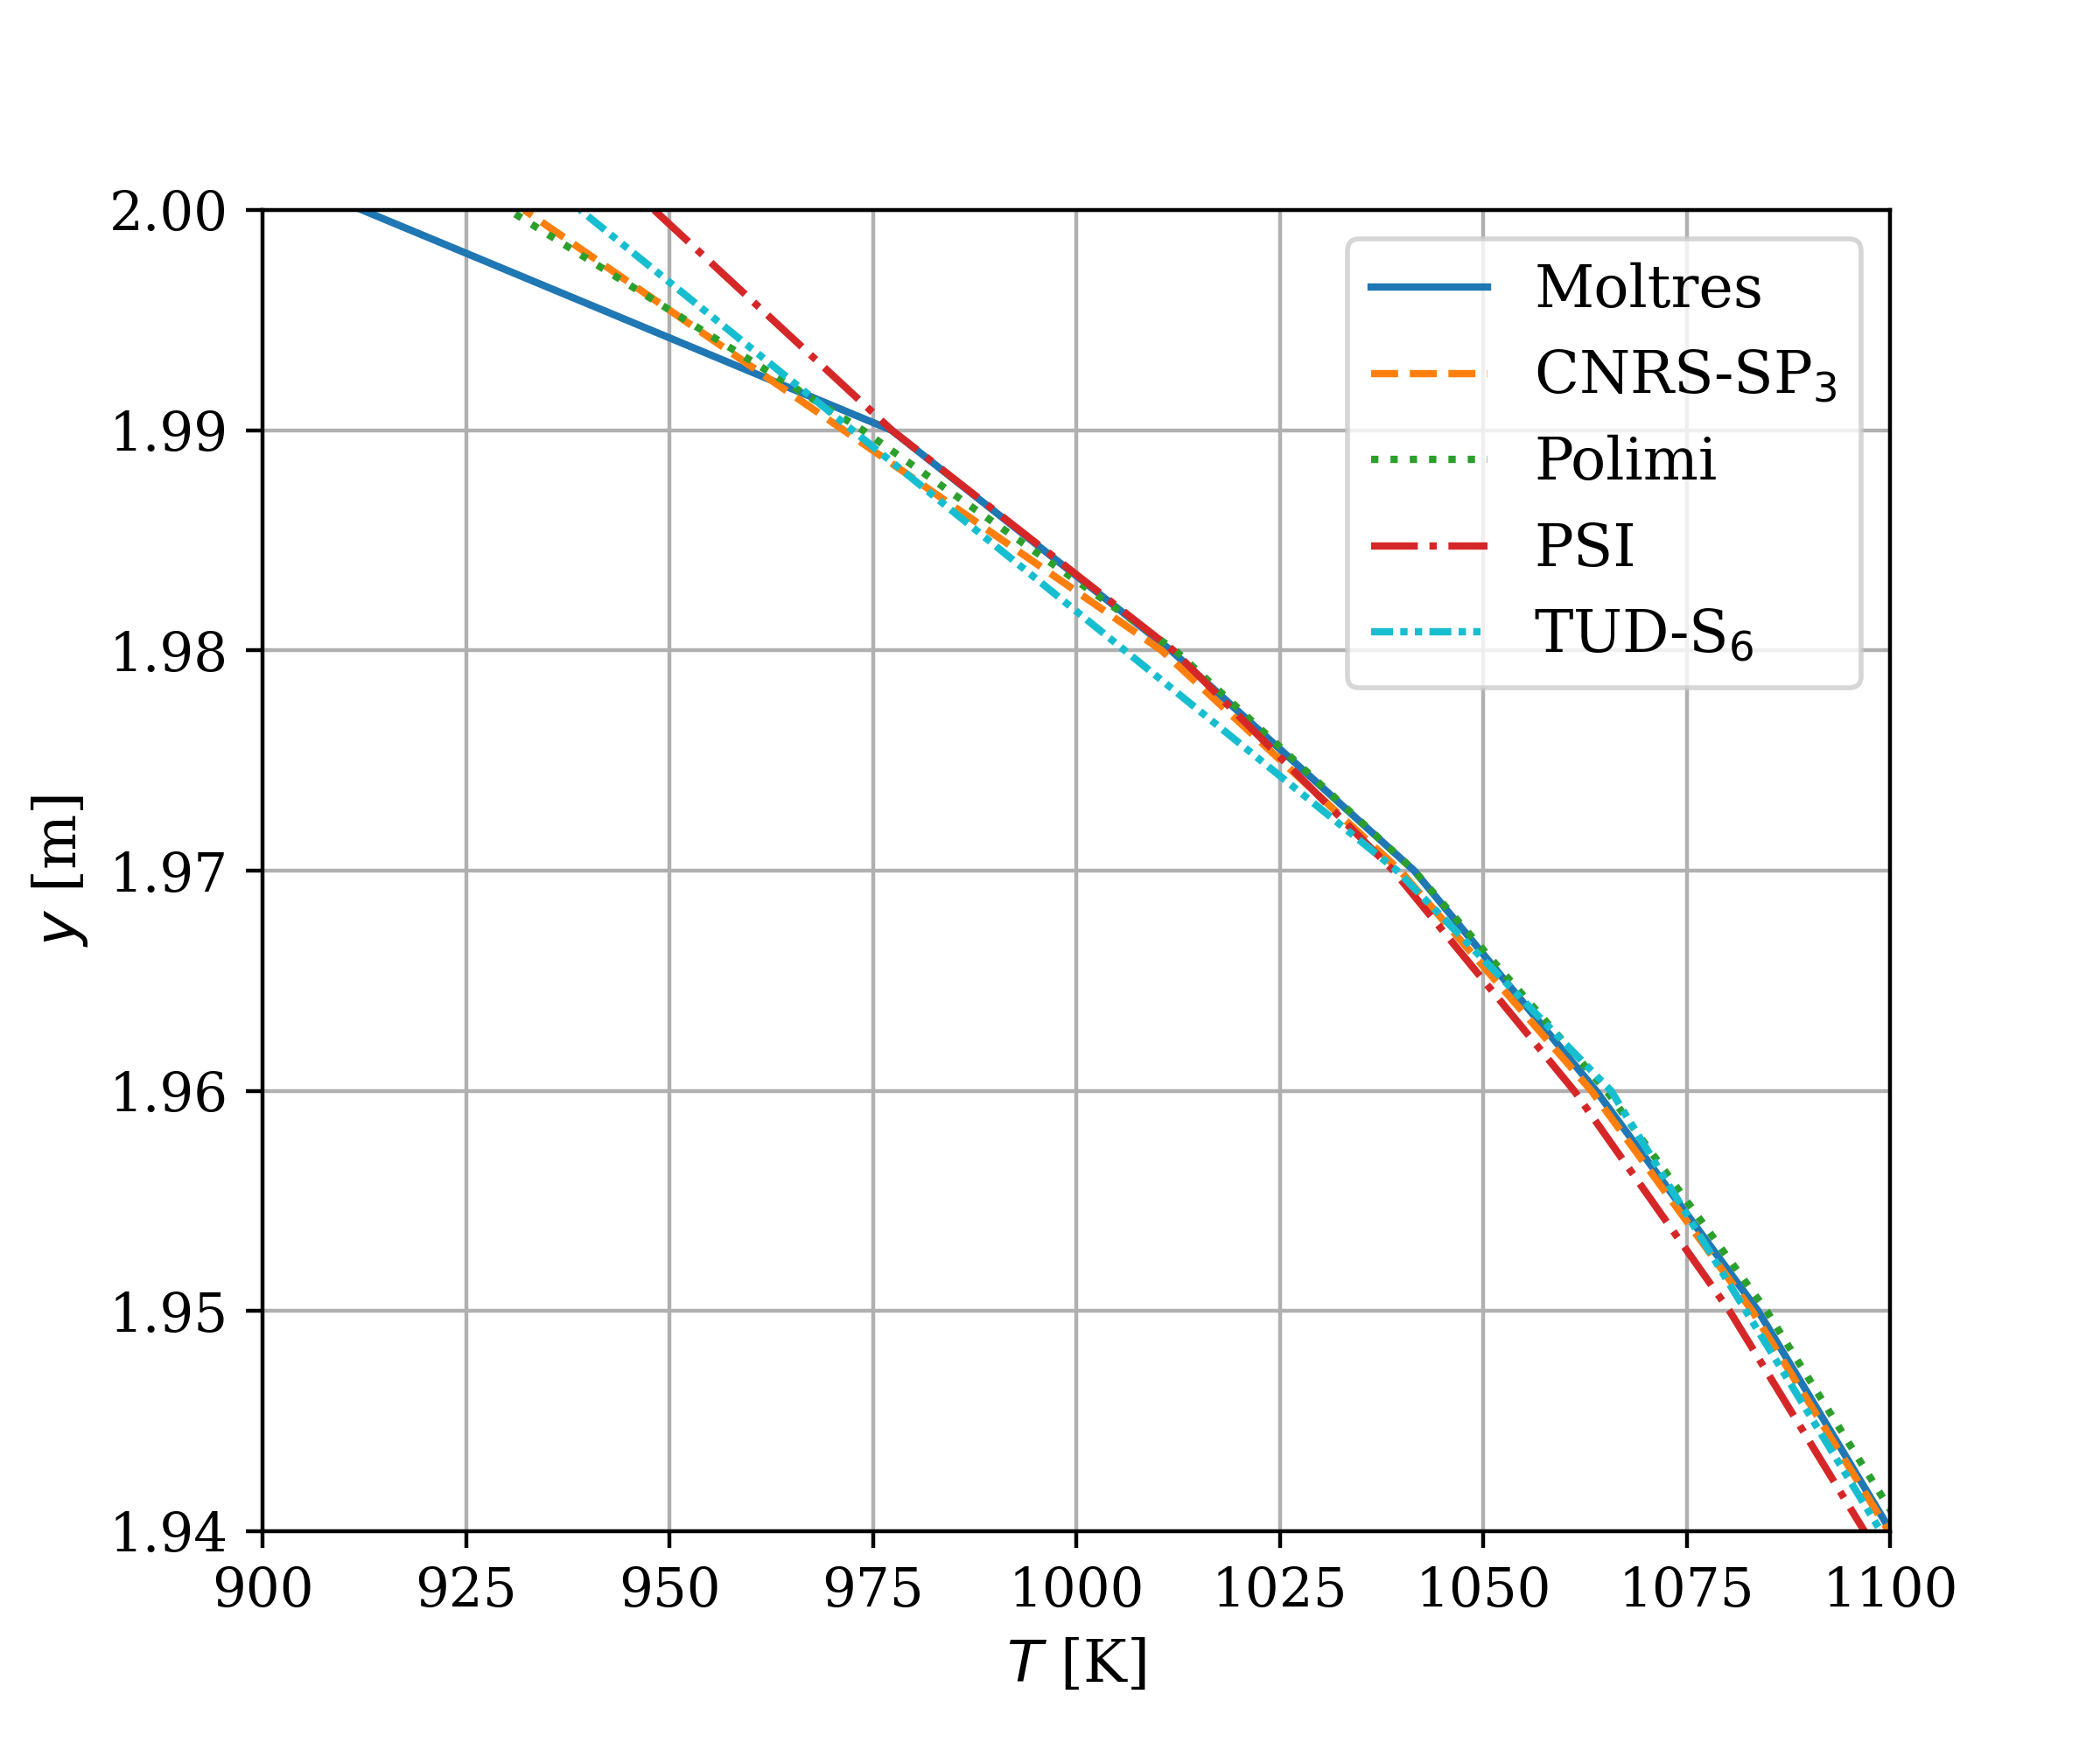
\includegraphics[width=.75\columnwidth]{0-3-temp-plot-zoom}
	\caption{Step 0.3 \textemdash\ Temperature distribution along BB' for y = 1.94 m to
	y = 2.00 m.}
	\label{fig:0.3-zoom}
\end{figure}

Lastly, we observe in table \ref{table:rho} that the reactivity $\rho$ value of
465.6 pcm from Moltres falls well within the range of $\rho$ values from the
benchmark which range from 353.7 pcm up to 578.1 pcm. Given that Moltres 
adopts the neutron diffusion model, our $\rho$ value agrees closest to the
results from the software packages which also adopt the neutron diffusion model
or theoretically-equivalent models such as the $SP_1$ and $S_2$ neutron
transport models, namely CNRS-$SP_1$, PoliMi, PSI, and TUD-$S_2$.

\begin{table}[htb]
    \caption{Reactivity $\rho$ and change in reactivity
    $\left(\rho_a - \rho_b\right)$ values from Steps 0.2, 1.1,
    1.2, and 1.3. All units are in pcm.}
    \centering
    \small
    \setlength\tabcolsep{2pt}
    \begin{tabular}{l S S S S}
        \toprule
        \multirow{2}{*}{\textbf{Software}} & {\textbf{Step 0.2}} &
        {\textbf{Step 1.1}} & {\textbf{Step 1.2}} & {\textbf{Step 1.3}} \\
        & {$\rho_{s_{0.2}}$}
        & {$\rho_{s_{1.1}} - \rho_{s_{0.2}}$}
        & {$\rho_{s_{1.2}} - \rho_{s_{1.1}}$}
        & {$\rho_{s_{1.3}} - \rho_{s_{0.2}}$} \\
        \midrule
        Moltres     & 465.6 & -62.7 & -1142.2 & -1207.7 \\
        CNRS-$SP_1$ & 411.3 & -62.5 & -1152.0 & -1220.5 \\
        CNRS-$SP_3$ & 353.7 & -62.6 & -1152.7 & -1220.7 \\
        PoliMi      & 421.2 & -62.0 & -1161.0 & -1227.0 \\
        PSI         & 411.7 & -63.0 & -1154.8 & -1219.6 \\
        TUD-$S_2$   & 482.6 & -62.0 & -1145.2 & -1208.5 \\
        TUD-$S_6$   & 578.1 & -60.7 & -1122.0 & -1184.4 \\
        \bottomrule
    \end{tabular}
    \label{table:rho}
\end{table}

\FloatBarrier

\subsection{Phase 1 results \& discussion}

Table \ref{table:disc1} shows the discrepancy values from Moltres relative to
the average and \gls{SD} of the benchmark participants for Steps 1.1, 1.2, and
1.3, and the corresponding average discrepancy values from the benchmark
\cite{tiberga_results_2020}. The subsequent subsections discuss the results
for each benchmark step in Phase 1.
%
\begin{table*}[htb]
	\caption{Discrepancy values from Moltres alongside the average and standard
	deviation of the discrepancy values of the benchmark participants for Phase
	1.}
	\centering
	\small
	\begin{tabular}{l l c S S S}
		\toprule
		\multirow{2}{*}{\textbf{Step}} & \multirow{2}{*}{\textbf{Observable}} & \multirow{2}{*}{\textbf{Centerline}} & {\multirow{2}{*}{\textbf{Moltres [\%]}}} & \multicolumn{2}{c}{\textbf{Benchmark [\%]}} \\
		& & & & {Average} & {SD} \\
		\midrule
		\multirow{2}{*}{1.1} &
		\multirow{2}{*}{$\sum_i \lambda_i C_i$} & AA' & 0.603 & 0.346 & 0.166
		\\
		& & BB' & 0.327 & 0.294 & 0.153 \\
		\midrule
		\multirow{4}{*}{1.2} &
		\multirow{2}{*}{$T$} & AA' & 0.076 & 0.095 & 0.015 \\
		& & BB' & 0.179 & 0.089 & 0.012 \\
		\cmidrule{2-6}
		& \multirow{2}{*}{\footnotesize $\Delta\left[\sum^6_g \Sigma_{f,g} \phi_g(\vec{r})
		\right]_{s_{1.2}-s_{0.2}}$} & AA' & 1.110 & 1.576 & 0.564 \\
		& & BB' & 1.089 & 1.133 & 0.392 \\
		\midrule
		\multirow{7}{*}{1.3} &
		{$u_x$} & AA' & 0.123 & 0.691 & 0.566 \\
		\cmidrule{2-6}
		& \multirow{2}{*}{$u_y$} & AA' & 0.237 & 0.329 & 0.131 \\
		& & BB' & 0.238 & 0.356 & 0.217 \\
		\cmidrule{2-6}
		& \multirow{2}{*}{$T$} & AA' & 0.064 & 0.057 & 0.023 \\
		& & BB' & 0.070 & 0.080 & 0.024 \\
		\cmidrule{2-6}
		& \multirow{2}{*}{$\sum_i \lambda_i C_i$} & AA' & 1.043 & 0.460 & 0.190
		\\
		& & BB' & 0.462 & 1.194 & 0.178 \\
		\bottomrule
	\end{tabular}
	\label{table:disc1}
\end{table*}

\subsubsection{Step 1.1: Circulating fuel}

Figure \ref{fig:1.1} shows good qualitative agreement in the delayed neutron
source distribution along BB' among Moltres and the benchmark participants.
From Table \ref{table:disc1}, Moltres reports discrepancies of 0.603\% and
0.327\% along the centerlines AA' and BB', respectively. Both values are on the
within two and one \gls{SD}, respectively, of the average discrepancies of the
benchmark participants (0.346\% and 0.294\%).
In Table \ref{table:rho}, we observe that the change in
$\rho$ relative to Step 0.2 is $-62.7$ pcm for Moltres and this value is
consistent with the $-63.0$ to $-62.0$ pcm range that most of the benchmark
participants' values fall in.
%
\begin{figure}[h!]
	\centering
    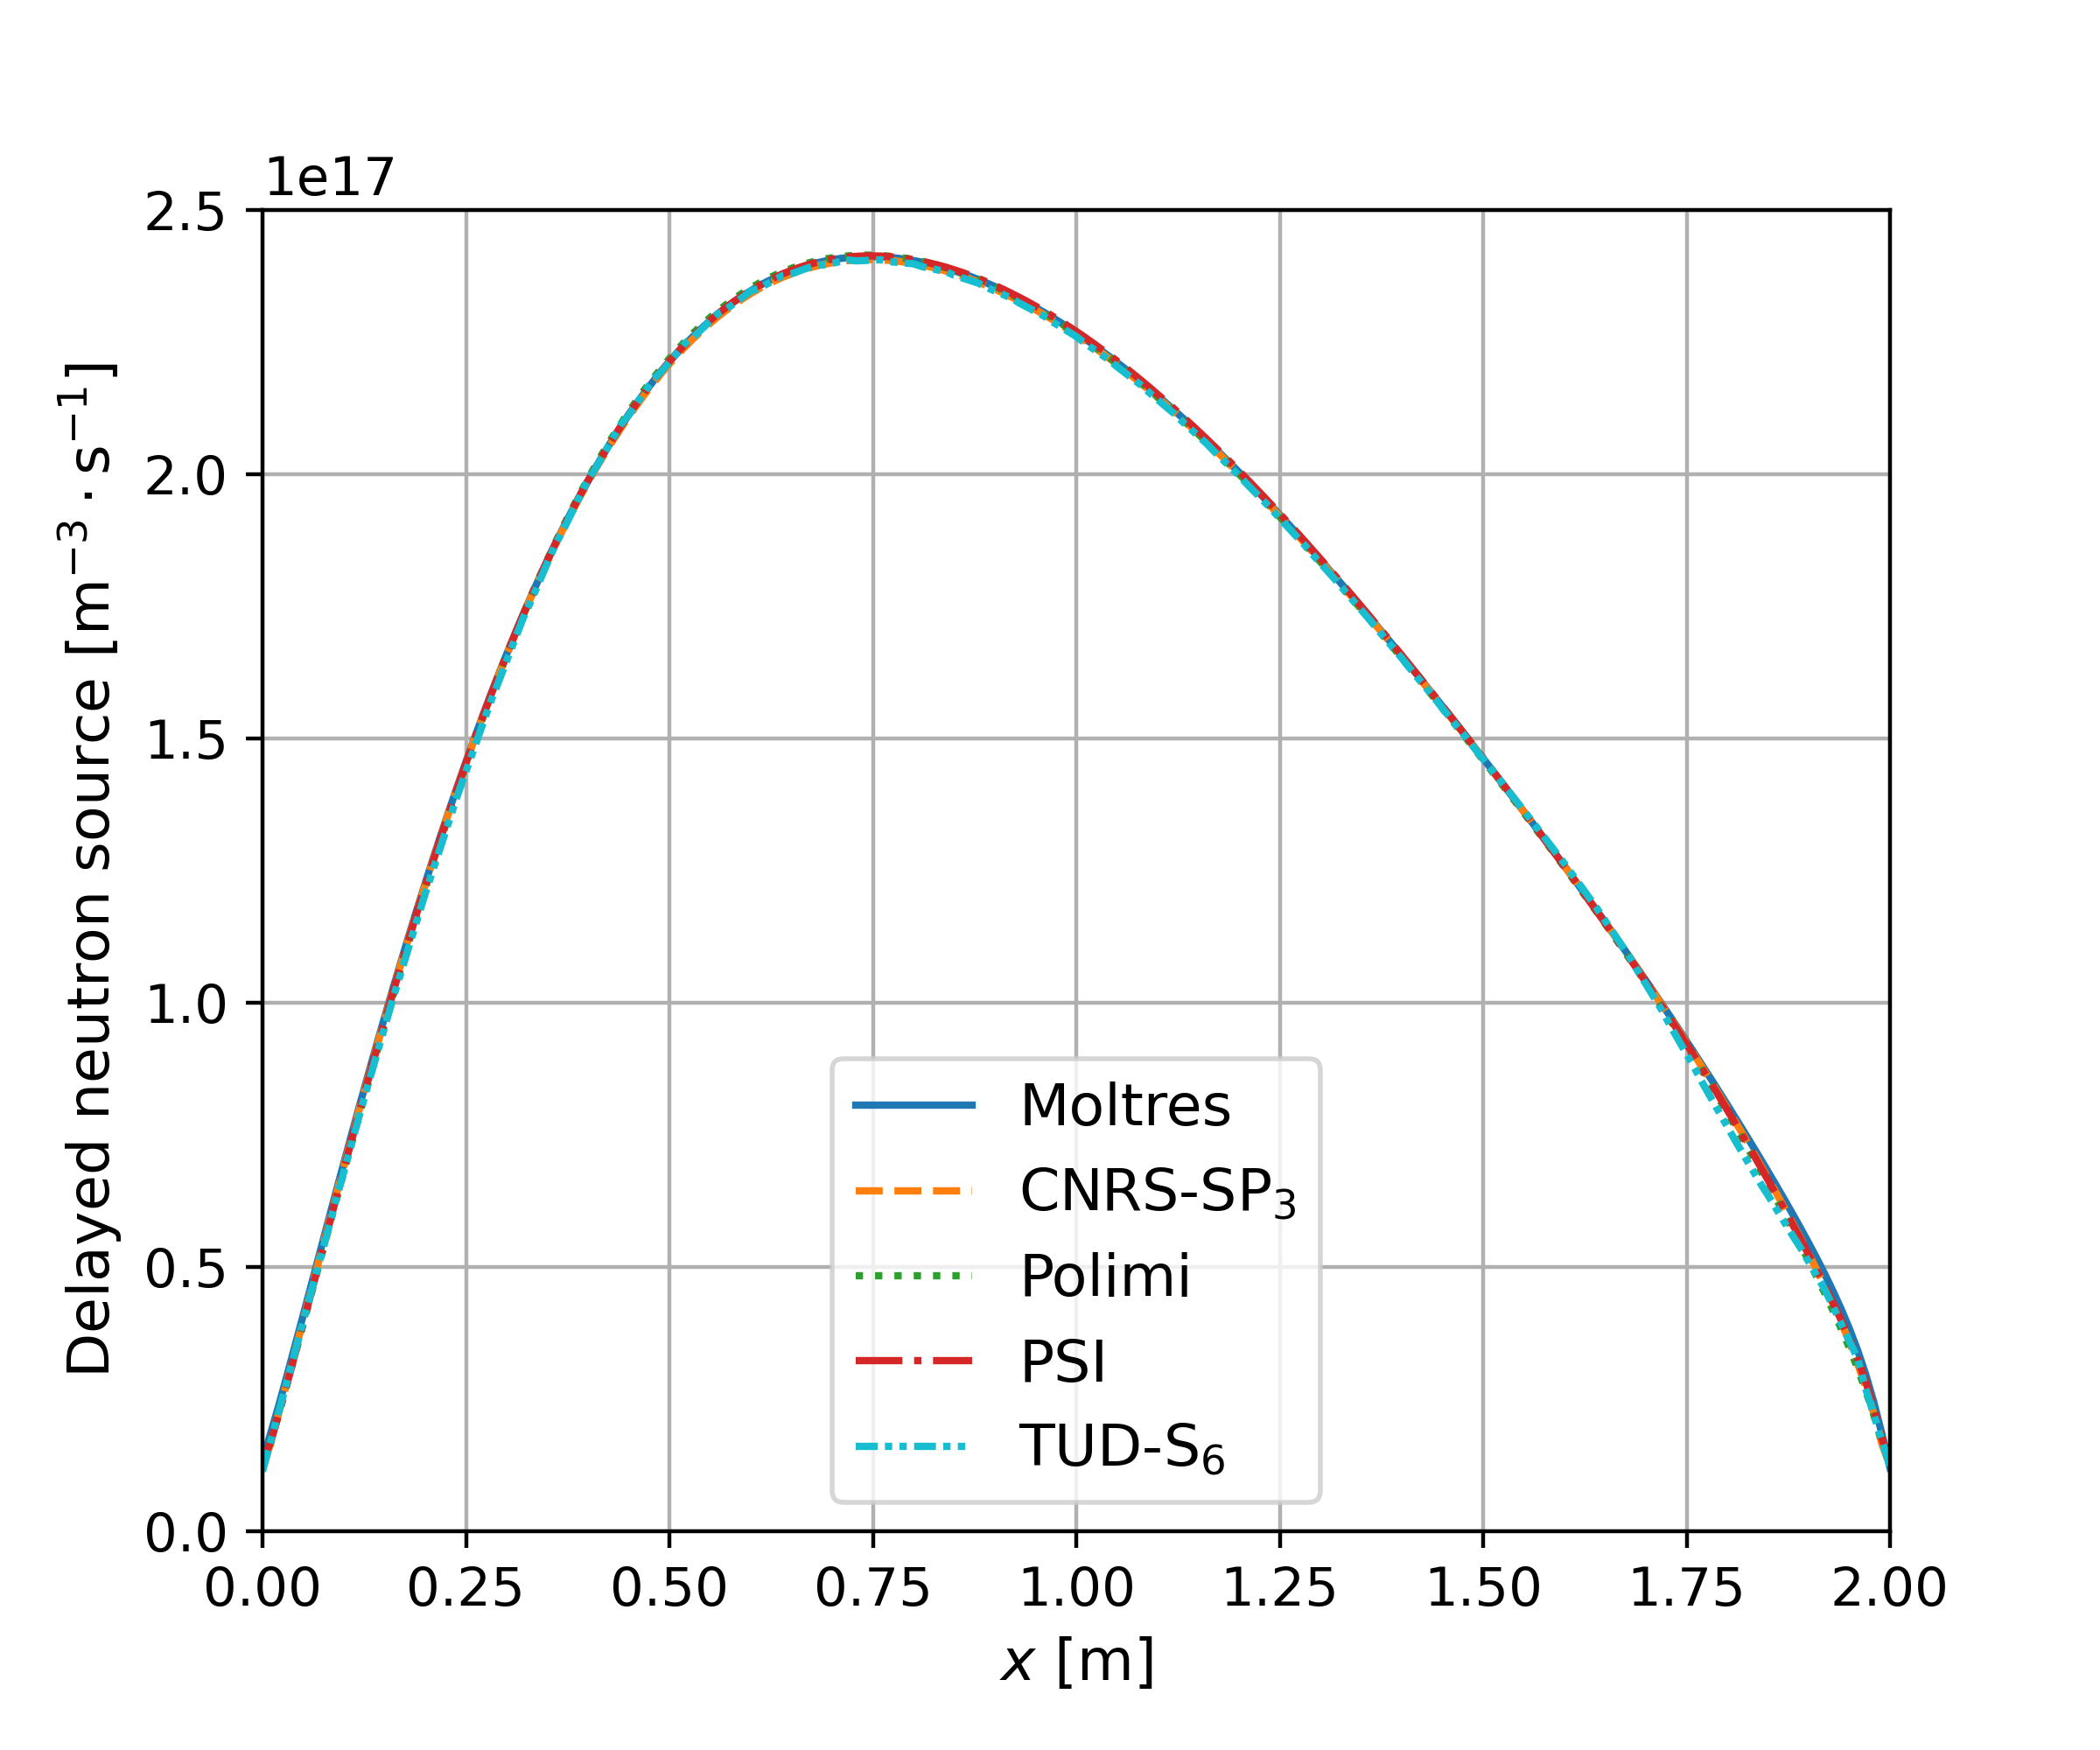
\includegraphics[width=.75\columnwidth]{1-1-dnp-x-plot}
    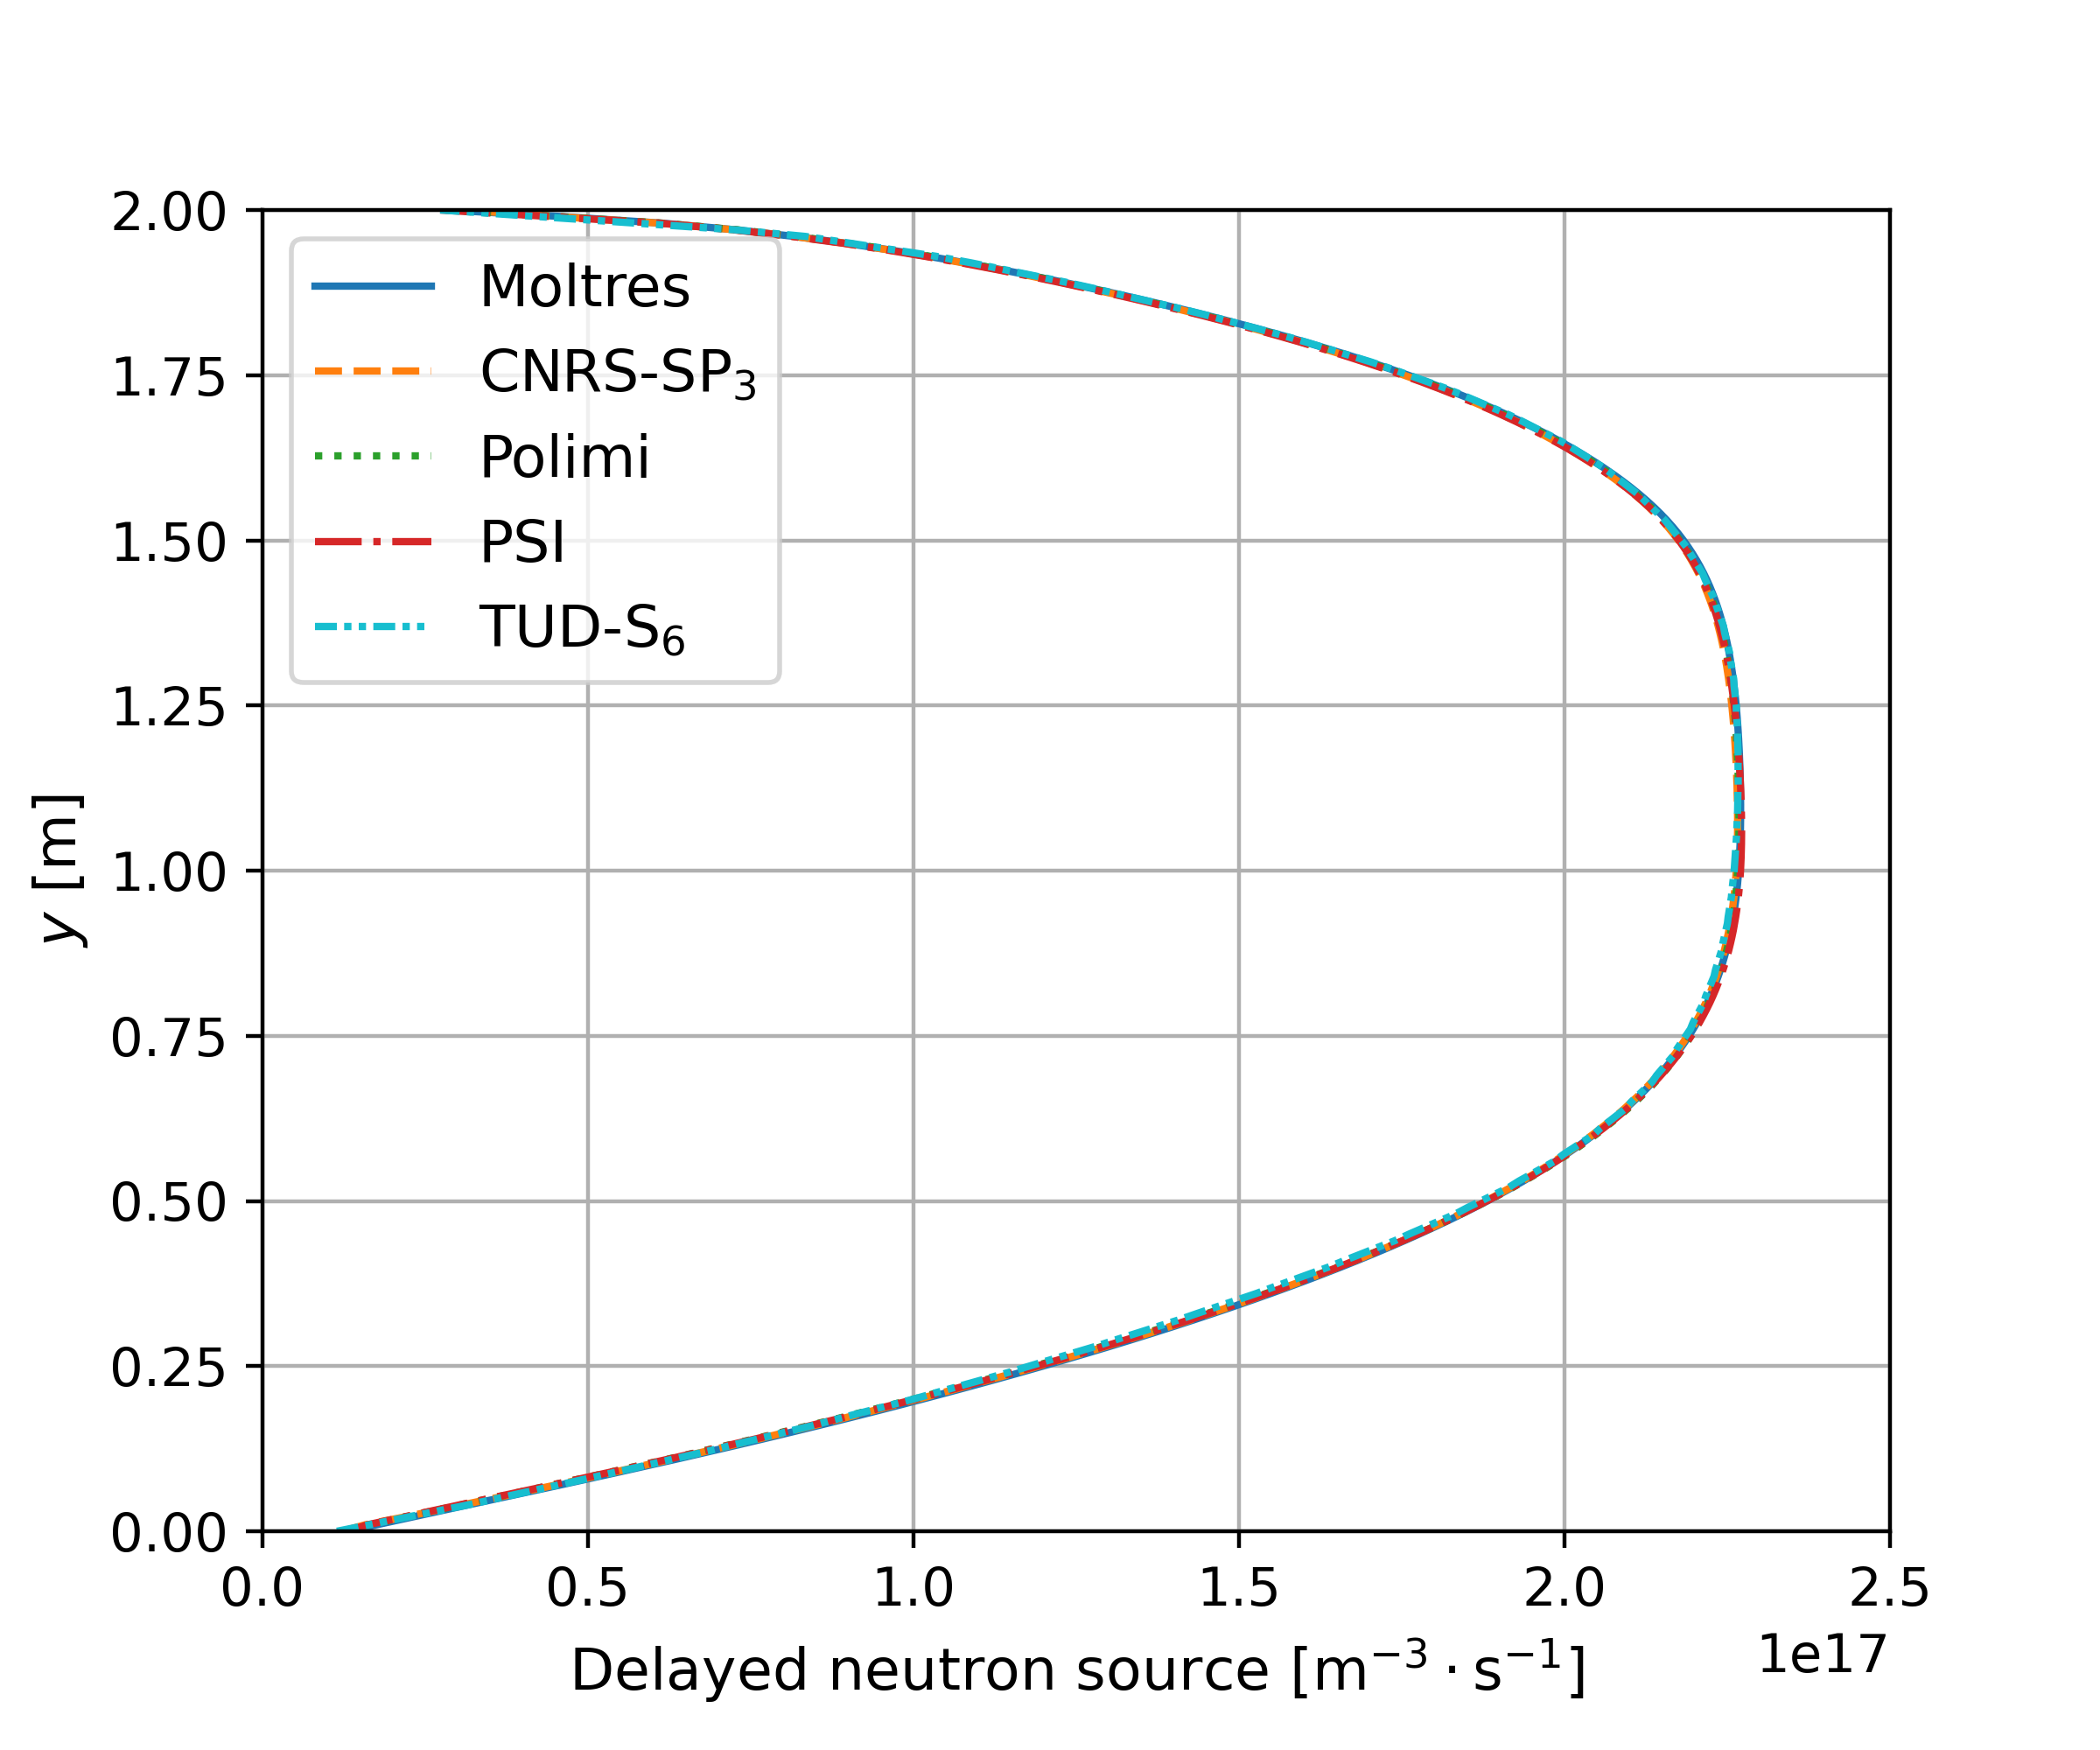
\includegraphics[width=.75\columnwidth]{1-1-dnp-y-plot}
	\caption{Step 1.1 \textemdash\ Delayed neutron source along AA' (top) and BB'
	(bottom).}
	\label{fig:1.1}
\end{figure}
%
\begin{figure*}[htb]
	\centering
	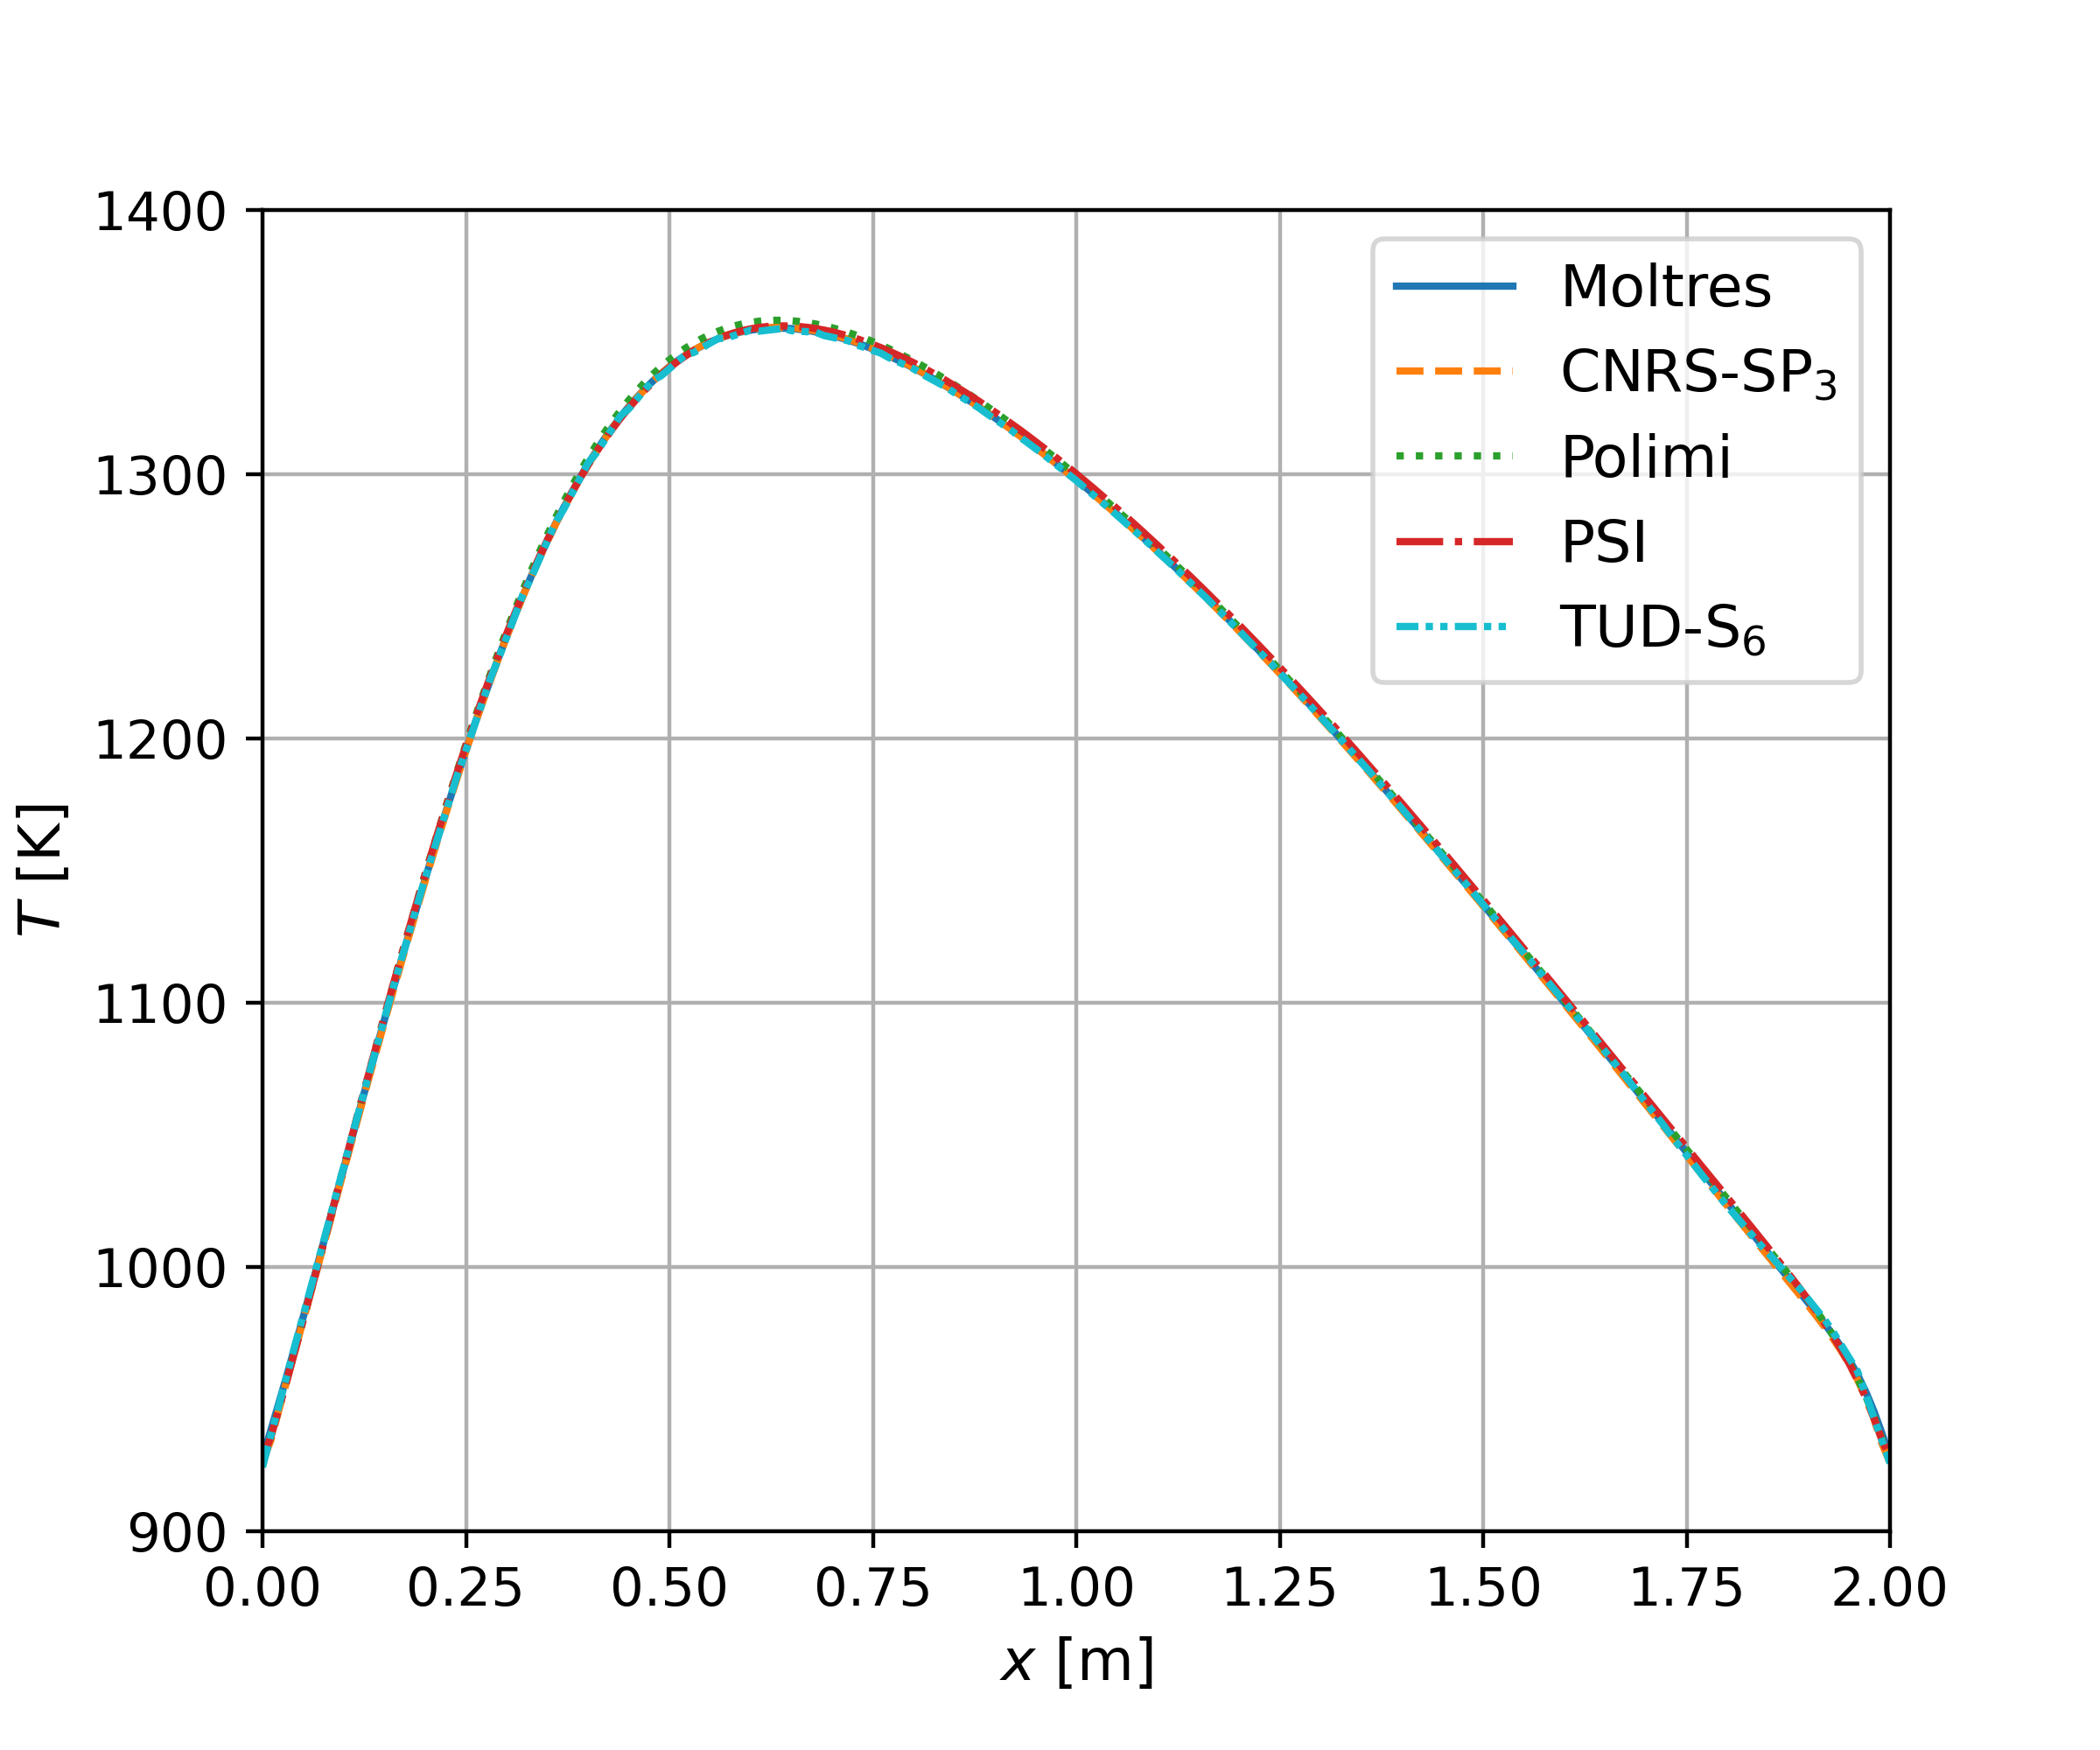
\includegraphics[width=.75\columnwidth]{1-2-temp-plot}
	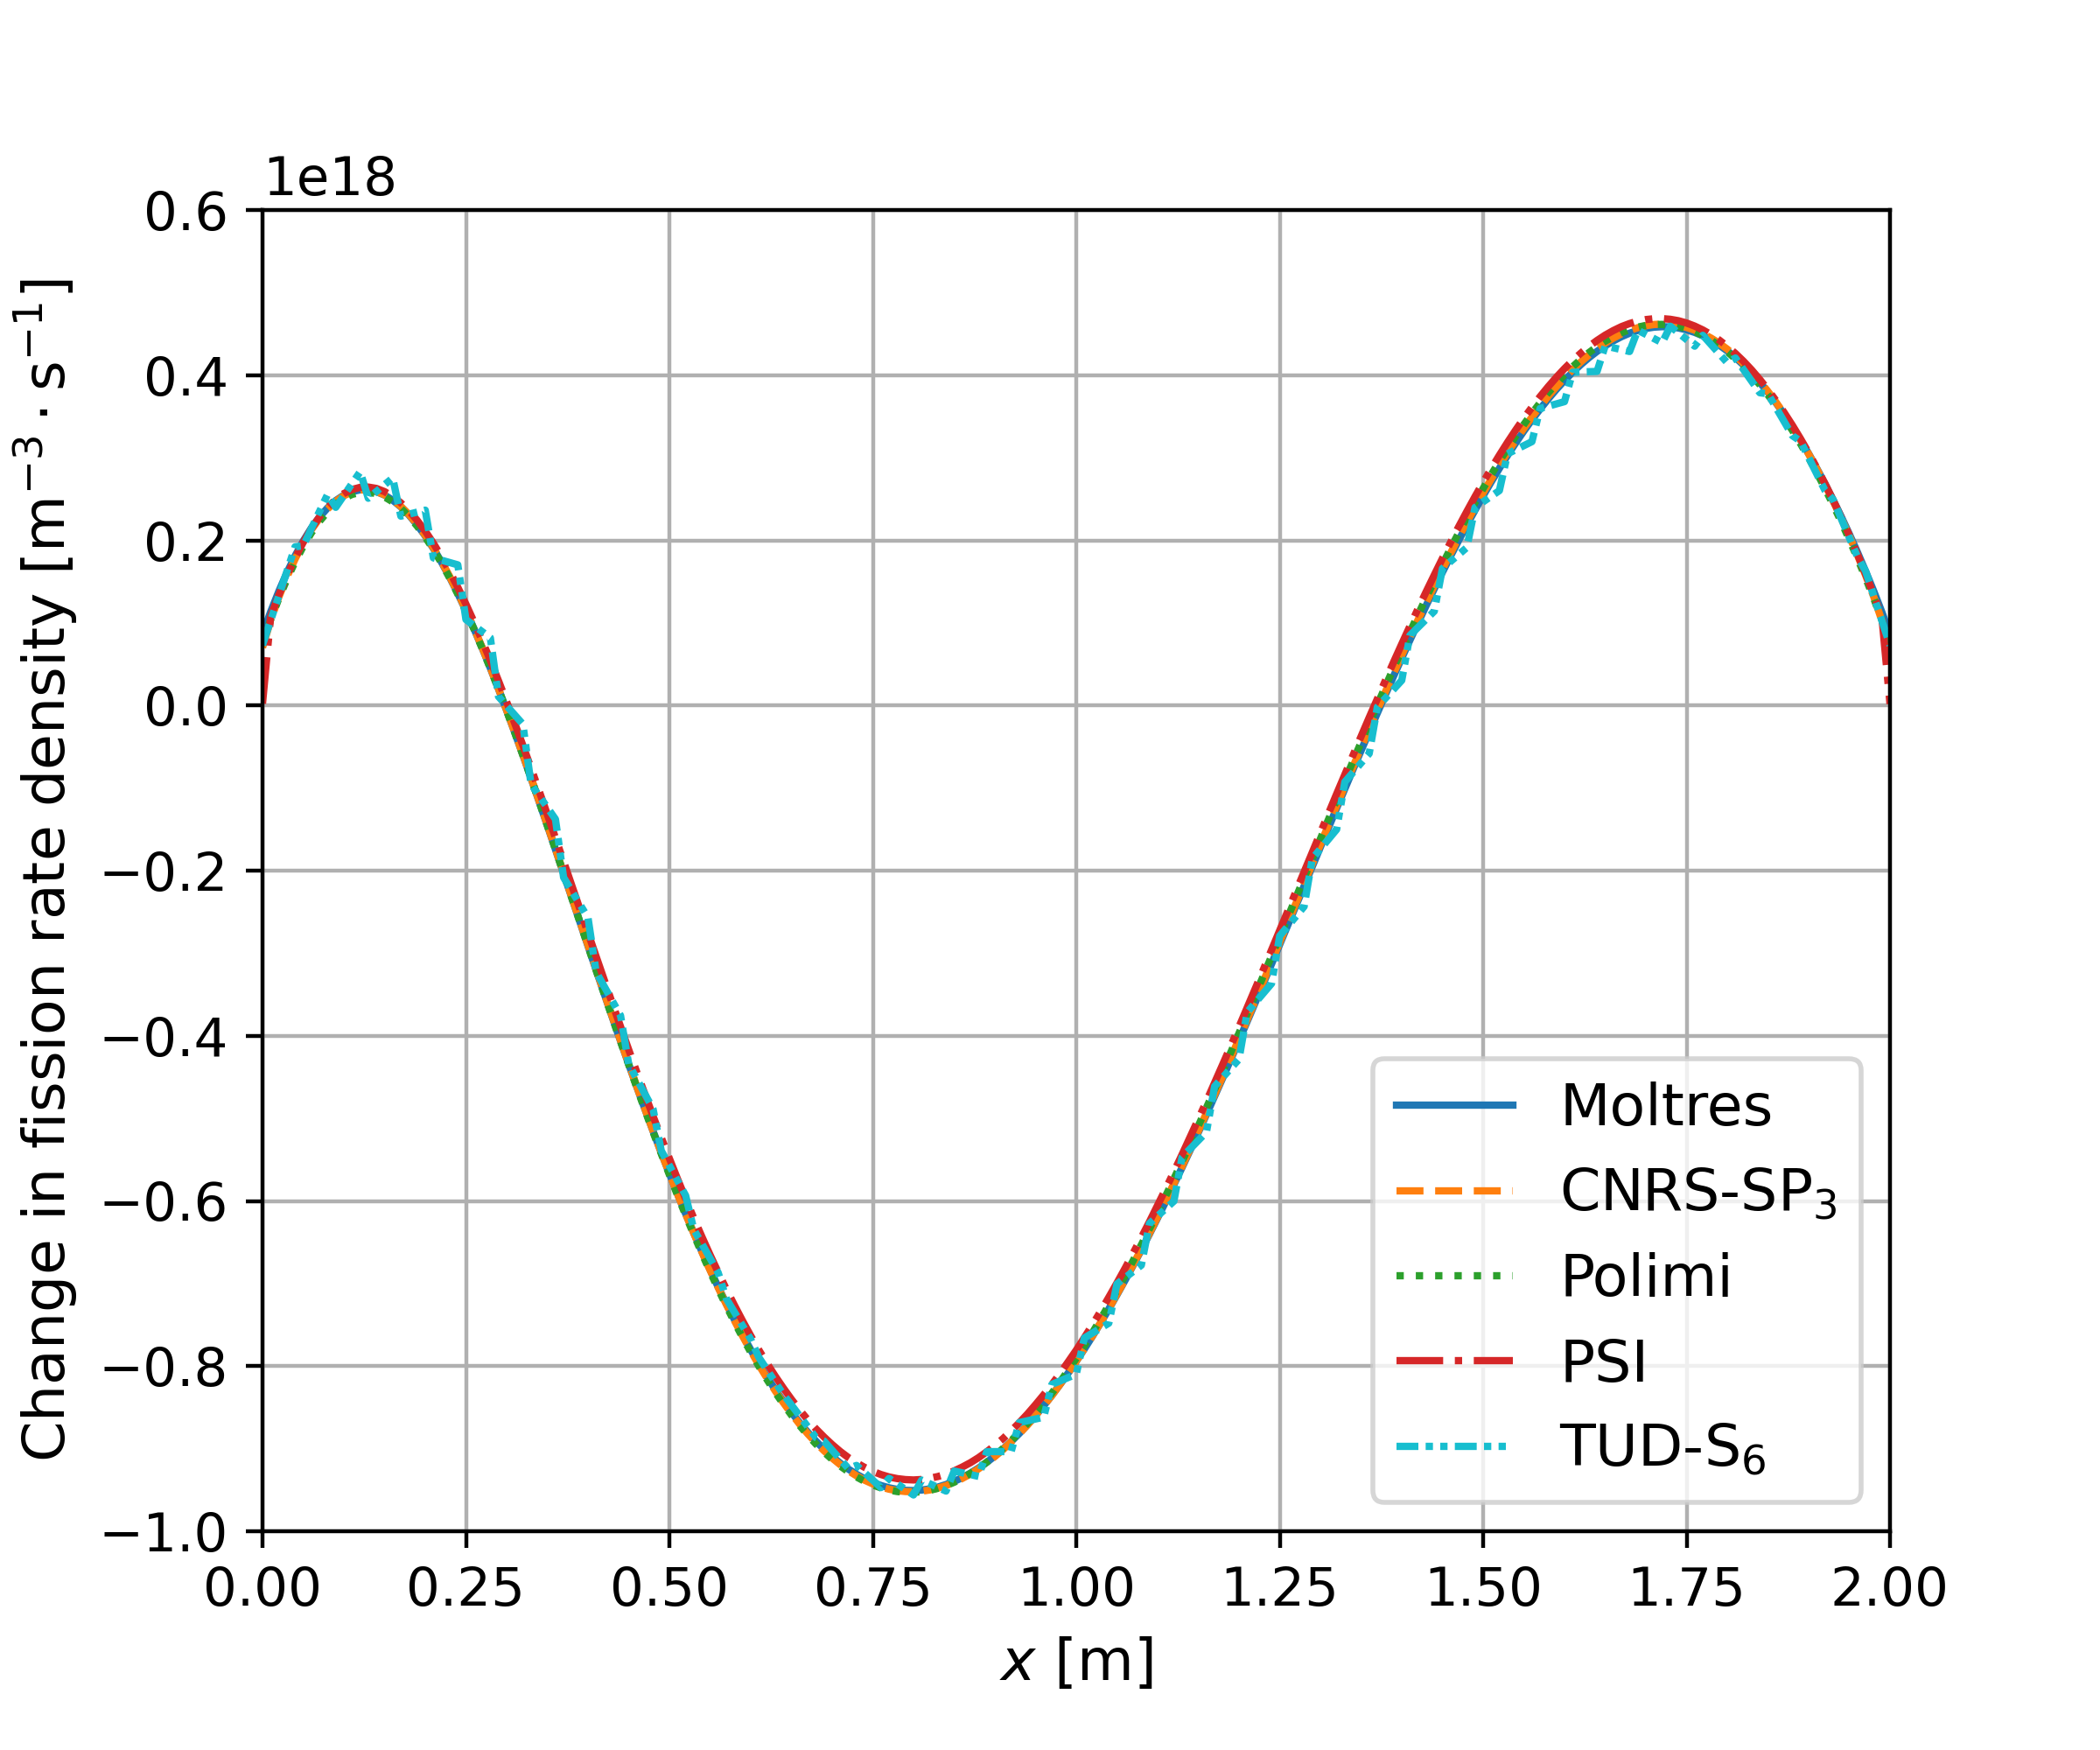
\includegraphics[width=.75\columnwidth]{1-2-fiss-plot}
	\caption{Step 1.2 \textemdash\ Temperature distribution and change in fission rate
	density along AA'.}
	\label{fig:1.2}
\end{figure*}

\FloatBarrier

\subsubsection{Step 1.2: Power coupling}

Figure \ref{fig:1.2} shows the temperature distribution and the change in
fission rate density along AA' from Step 1.2. Similar to Step 0.3, the
temperature distribution from Moltres agrees closest with CNRS-$SP_3$ and
TUD-$S_2$. Table \ref{table:disc1} reports the same trends we observed in Phase
0; the average discrepancy in temperature along BB' from Moltres for Step 1.2
is marginally higher than the benchmark while the average discrepancy in the
fission rate density is within one \gls{SD} range to the benchmark average.
From Table \ref{table:rho}, Moltres also reports a change in $\rho$
relative to Step 1.1 of $-1142.2$ pcm which
falls within the range of reported benchmark participants' values.

\subsubsection{Step 1.3: Buoyancy}

Figure \ref{fig:1.3} shows the vertical velocity component, temperature, and
delayed neutron source distributions along AA'.
Moltres reproduces the correct trend in all three physical
observables. Step 1.3 has a relatively slower buoyancy-driven flow profile with
no forced flow from the top boundary. Consequently, there are no temperature
deviations near the top boundary and we observe in Table \ref{table:disc1} that
the average discrepancy value of 0.070\% for the temperature distribution along
BB' is in much closer agreement to the benchmark value of 0.080\% compared to
the corresponding temperature discrepancy values for Step 0.3 and 1.2.

In Table \ref{table:rho}, we observe that the change in $\rho$ from
Moltres (-1207.7 pcm) falls within the range of reported benchmark values and
matches the software from TUD-$S_2$ (-1208.5 pcm) the closest. This is likely
by virtue of the similar solvers (diffusion and $S_2$ neutronics models) and
methods of solution (finite element method on uniform meshes) employed by our
respective software.
%
\begin{figure*}[htb]
	\centering
	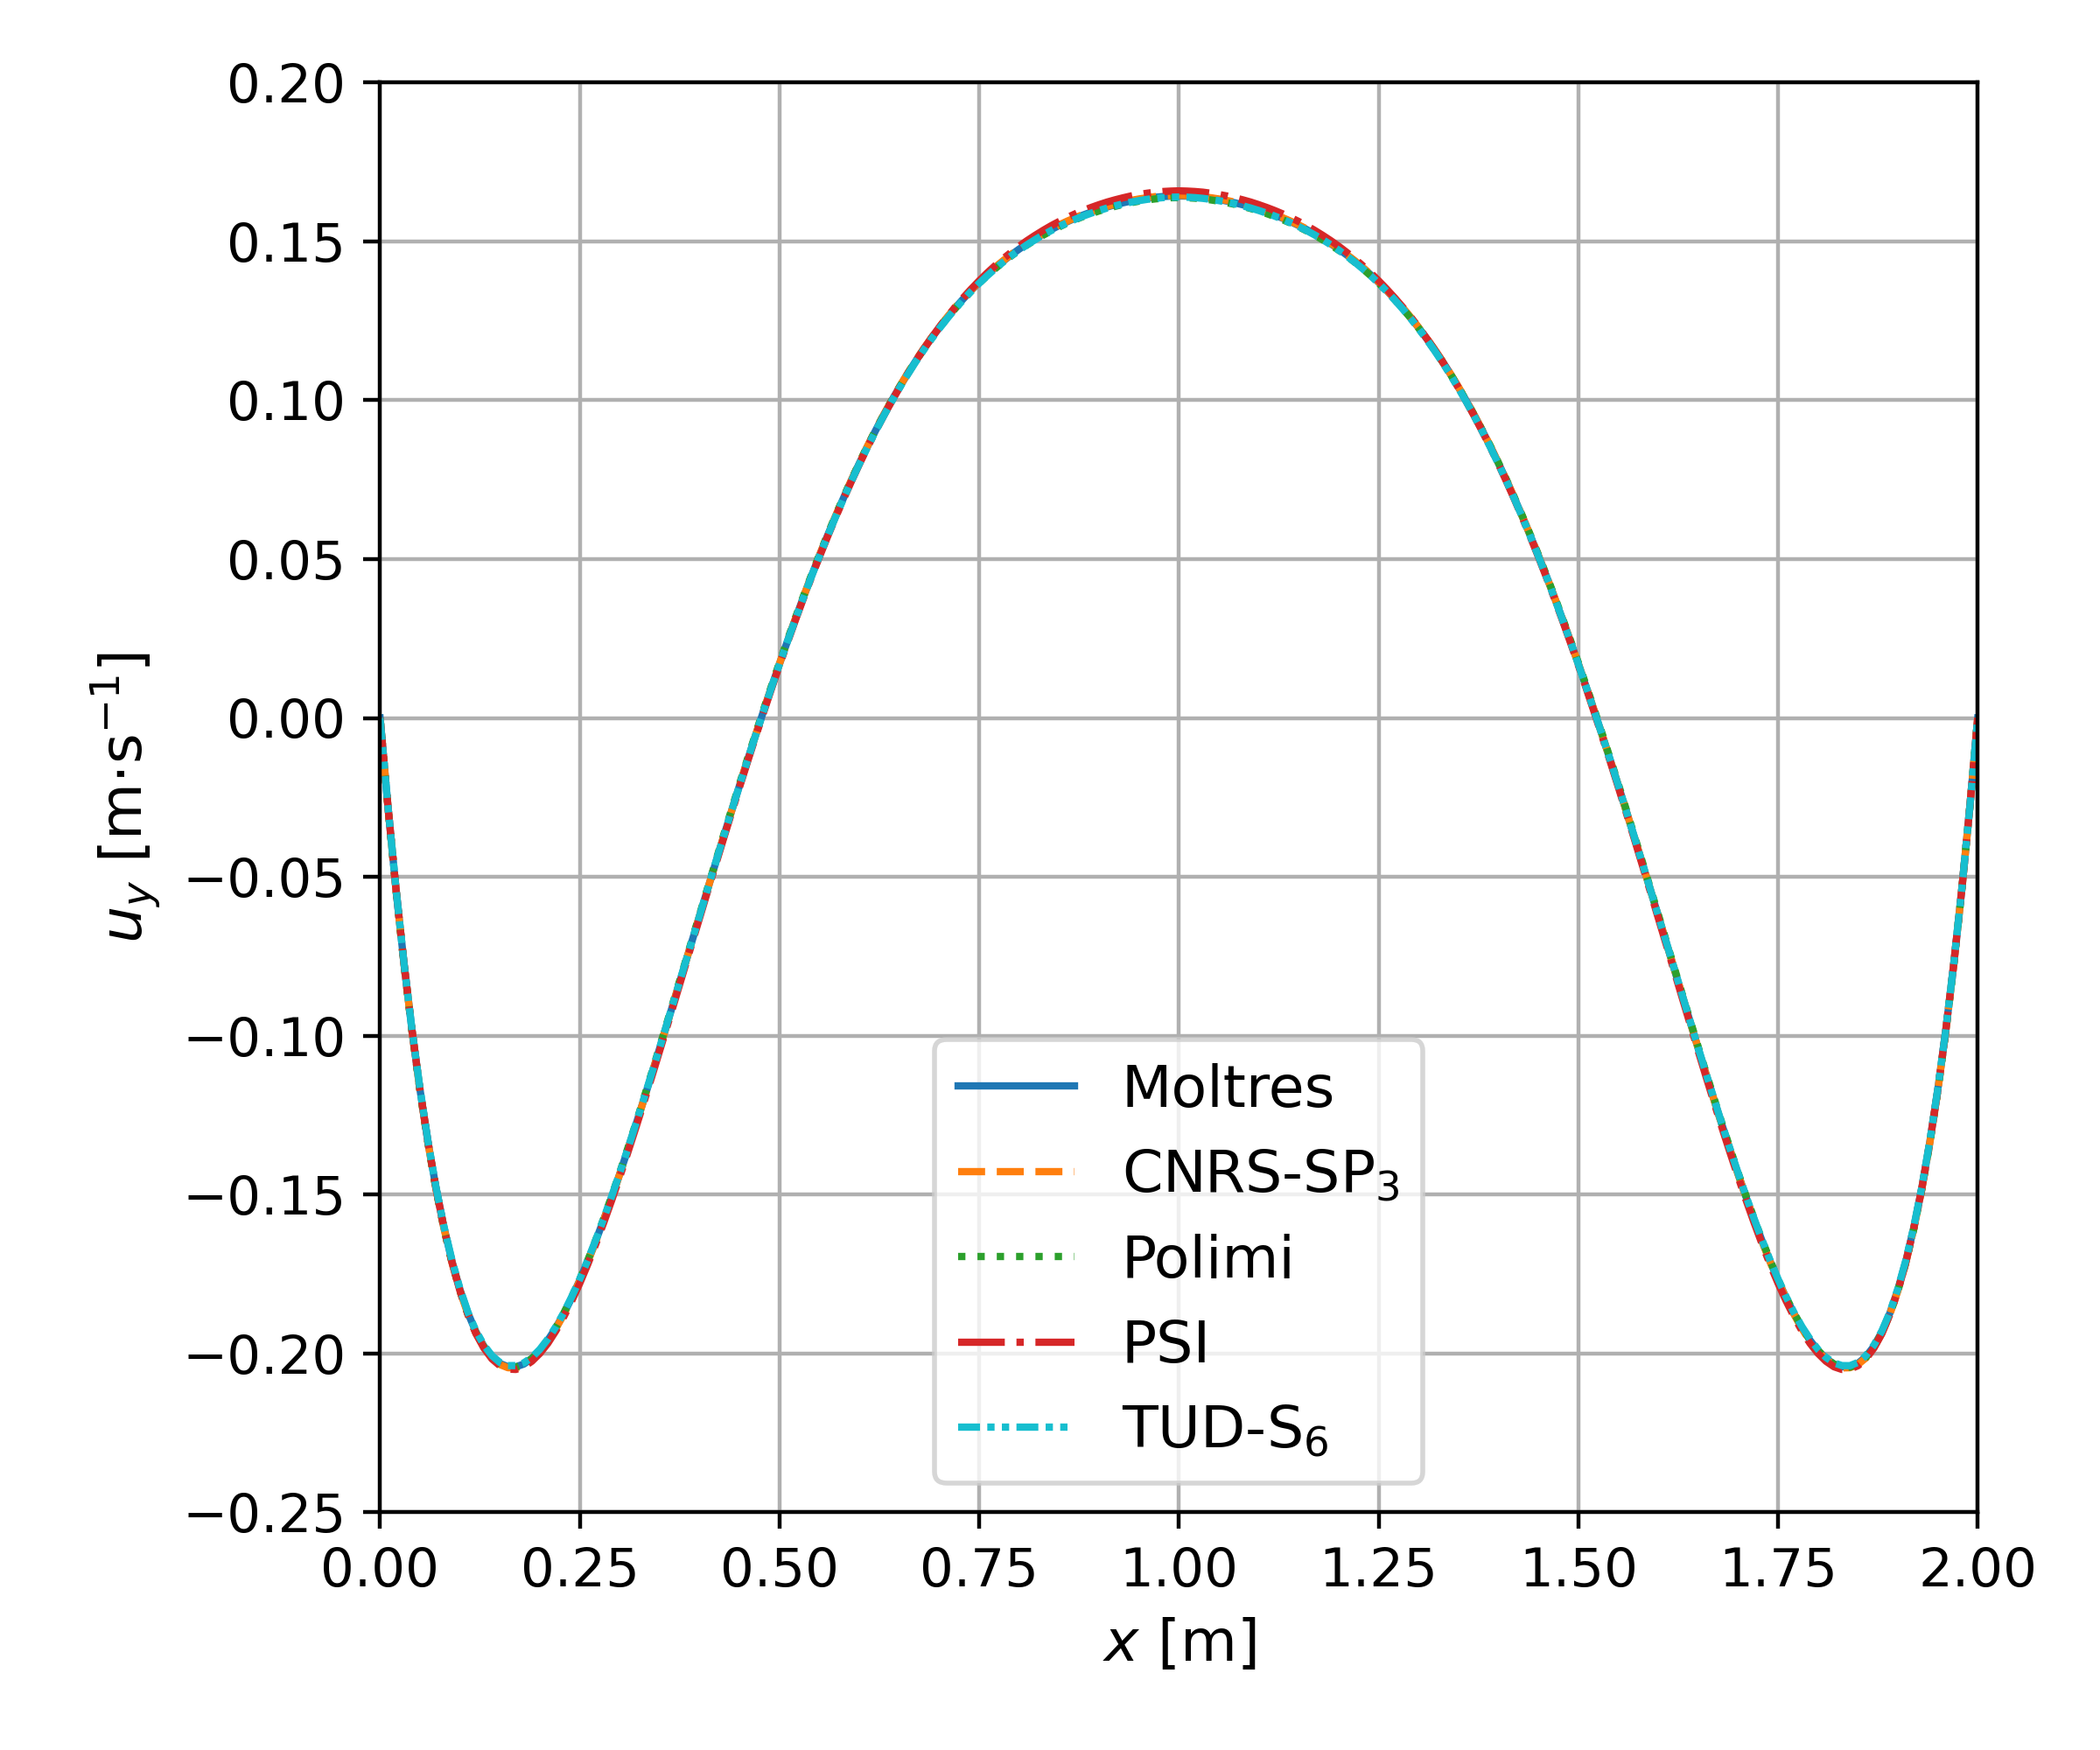
\includegraphics[width=.5\columnwidth]{1-3-vel-plot}
	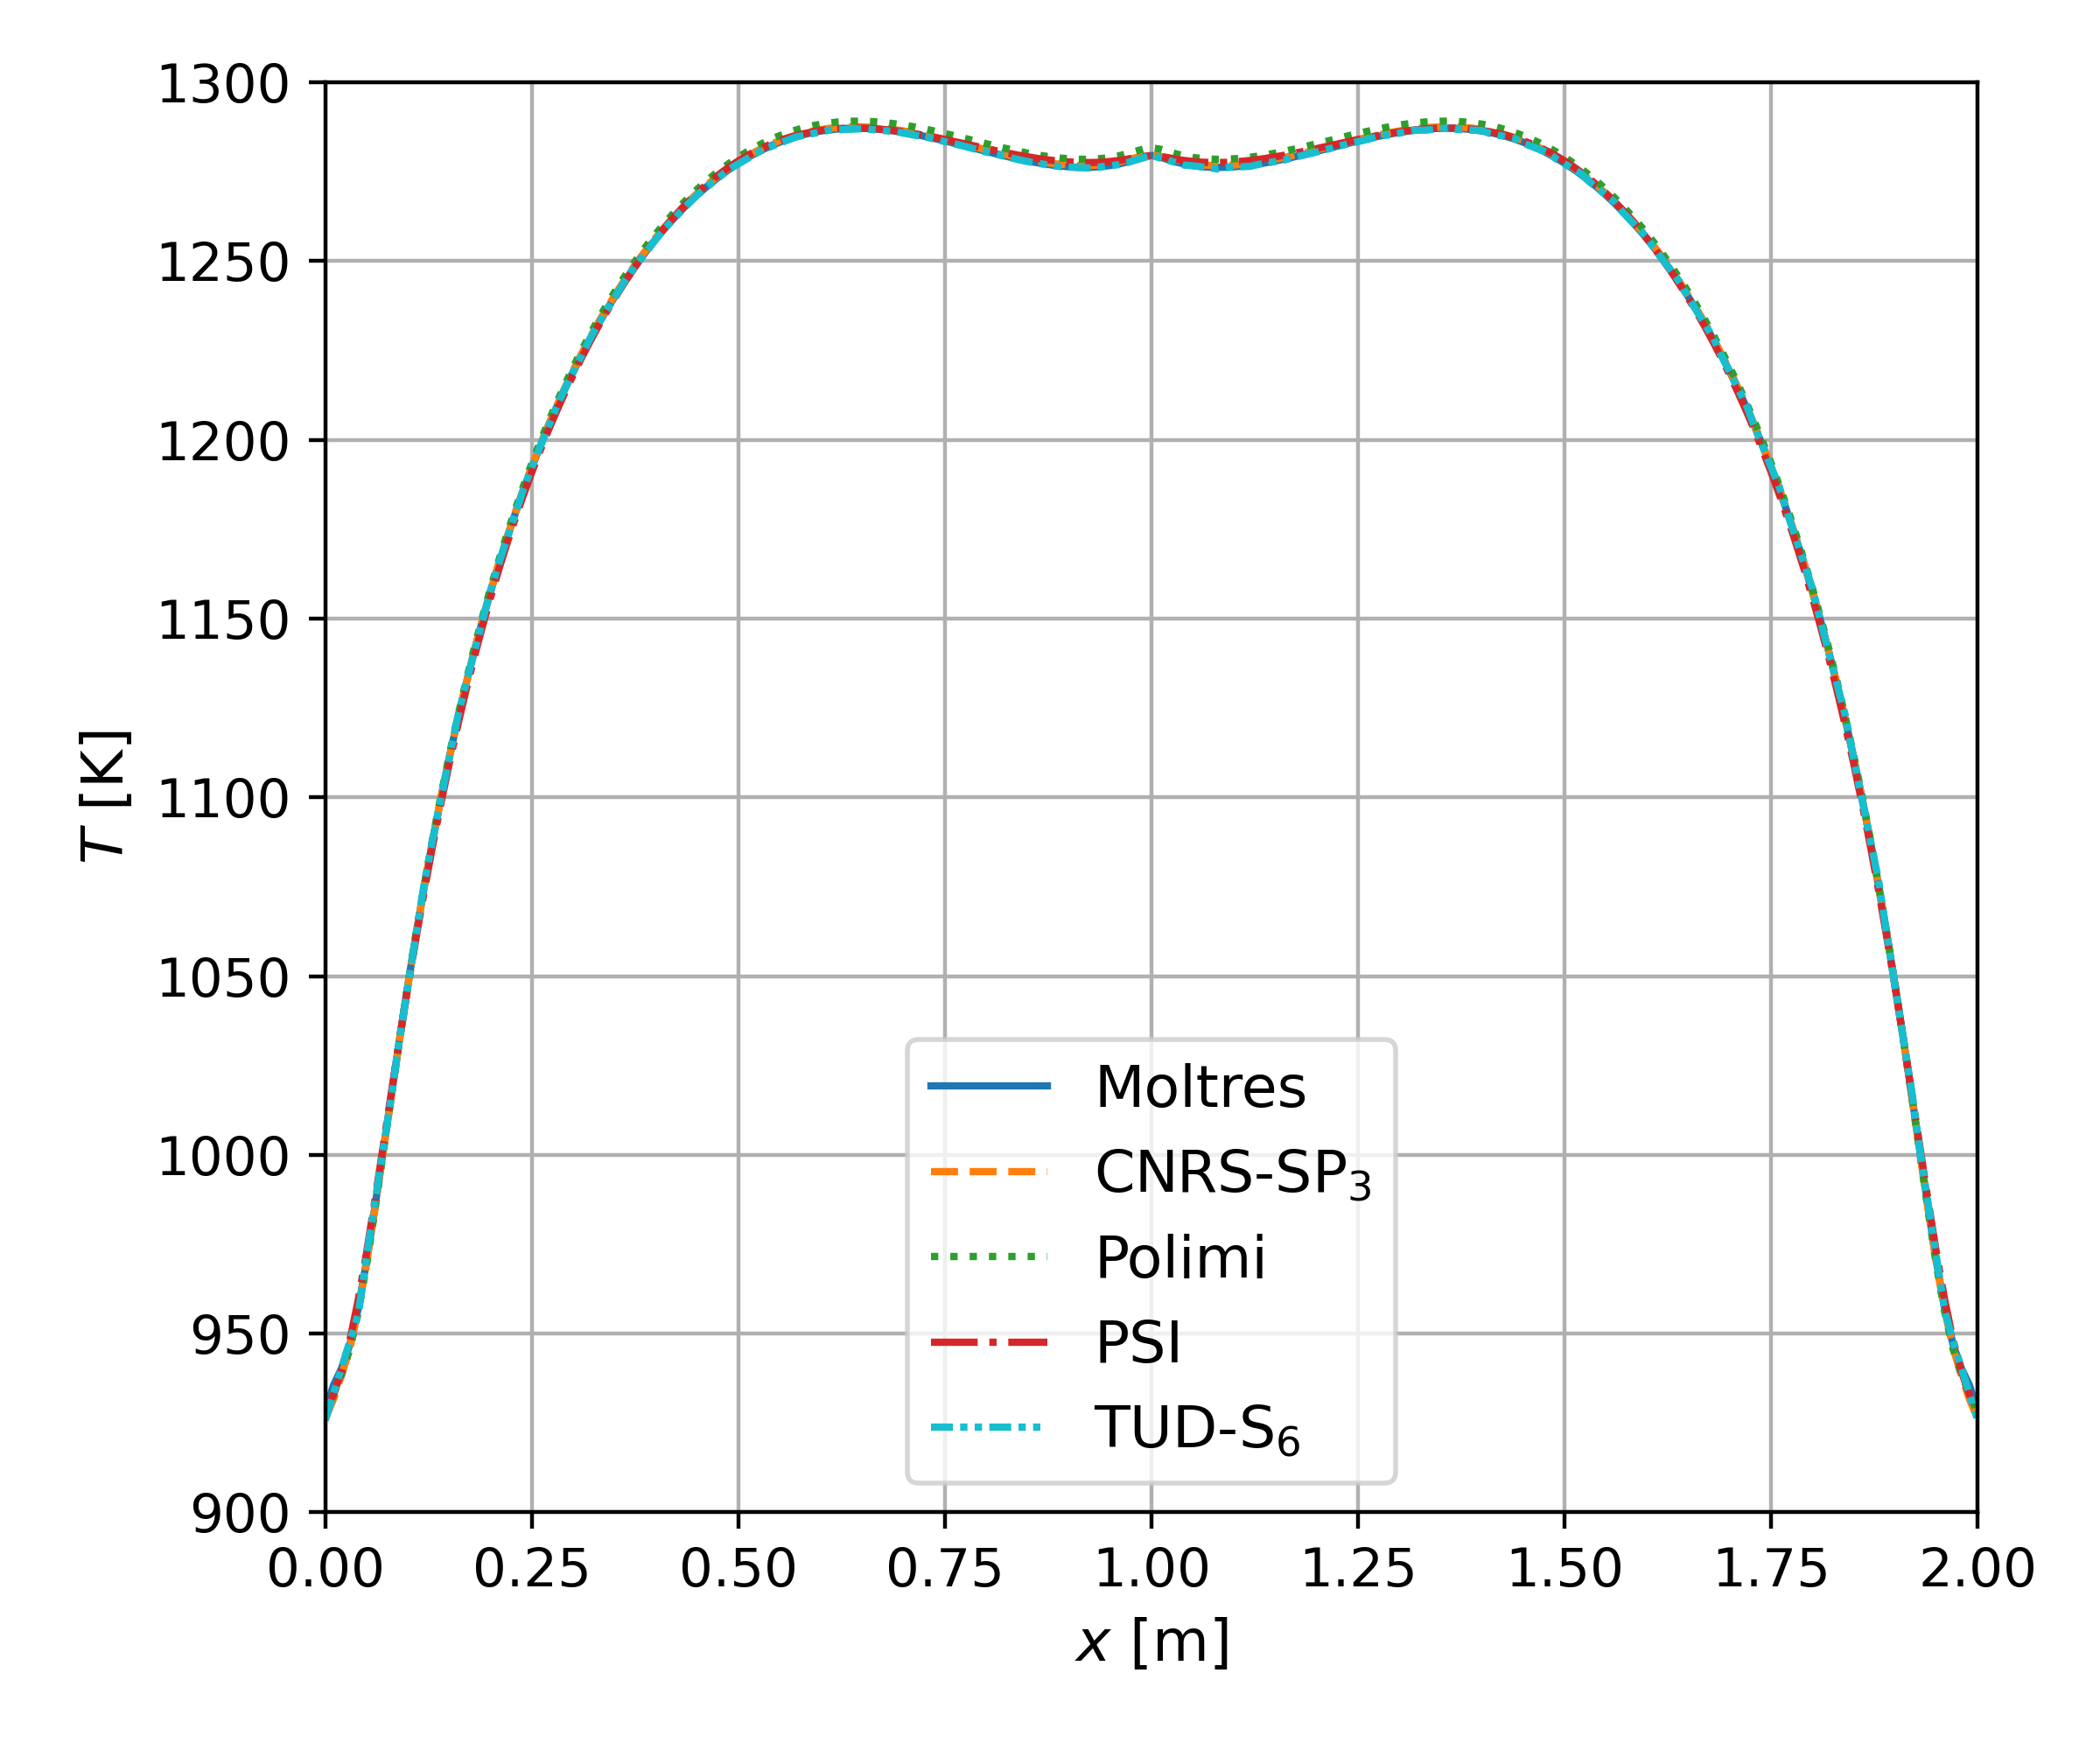
\includegraphics[width=.5\columnwidth]{1-3-temp-plot}
	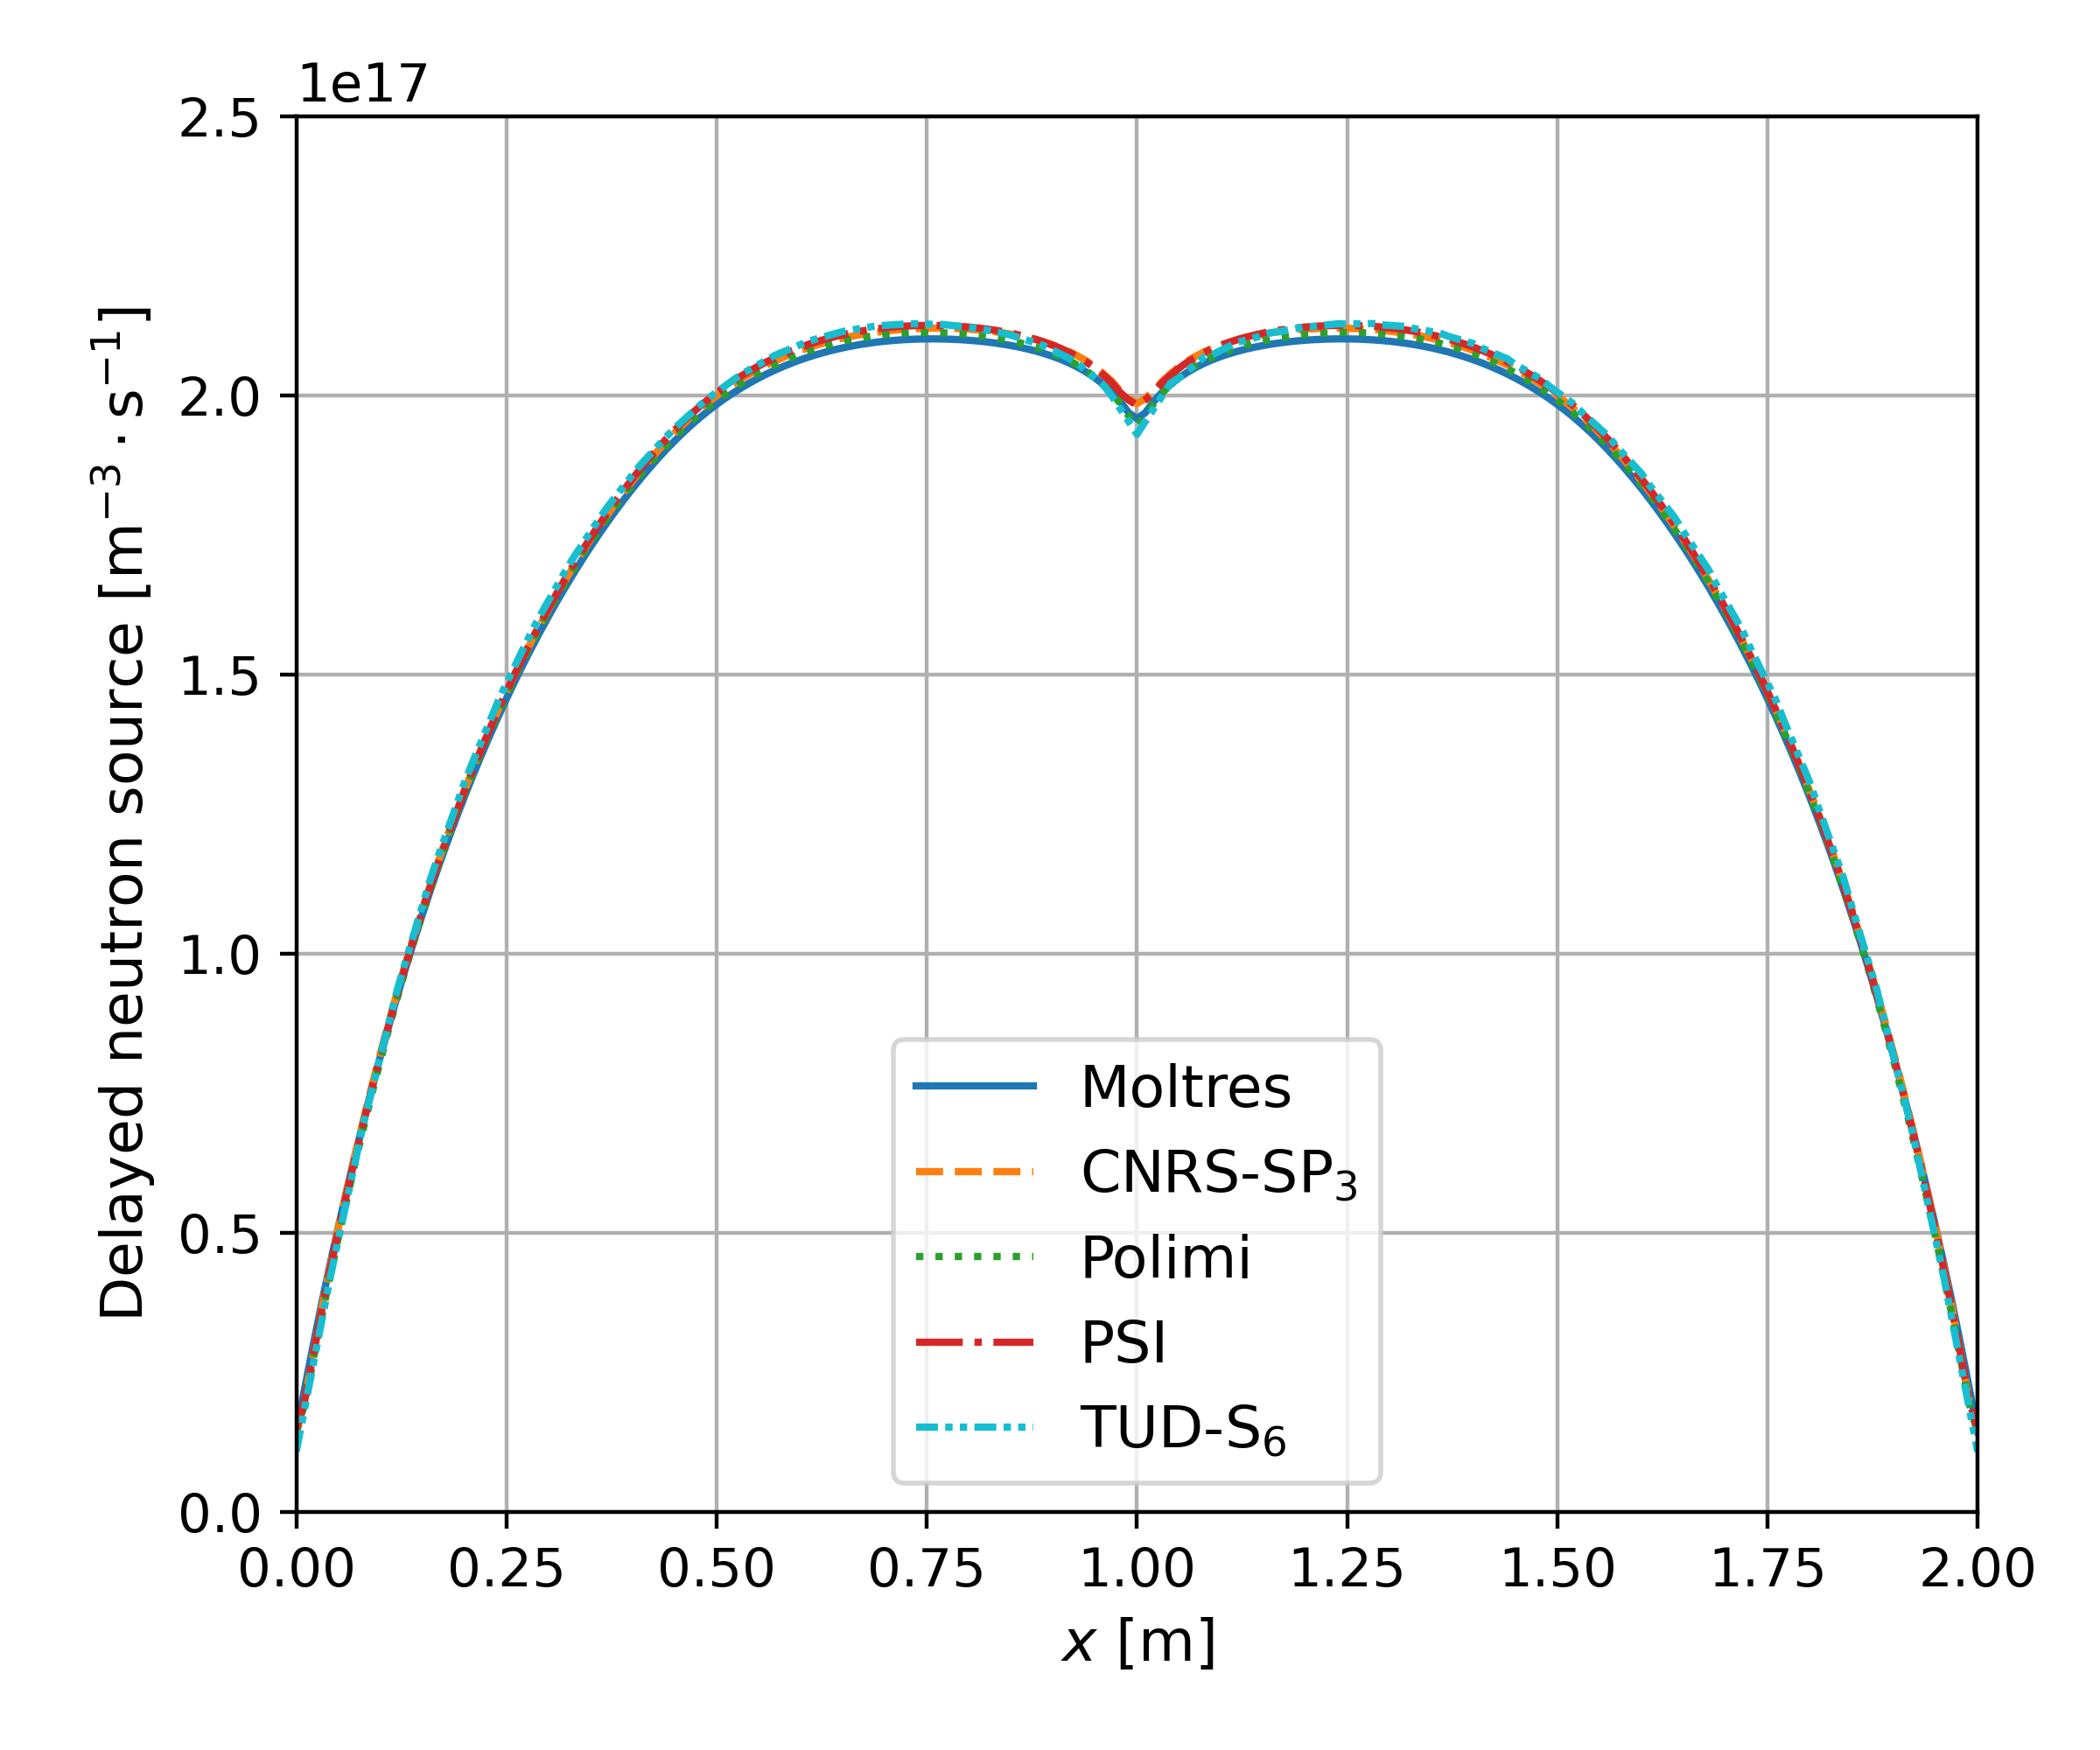
\includegraphics[width=.5\columnwidth]{1-3-dnp-plot}
	\caption{Step 1.3 \textemdash\ Vertical velocity component, temperature distribution,
	and delayed neutron source along AA'.}
	\label{fig:1.3}
\end{figure*}

\FloatBarrier

\subsubsection{Step 1.4: Full coupling}

Figure \ref{fig:cnrs-color} shows 2D temperature distribution and velocity
streamlines from Moltres for Step 1.4 with $U_{lid} = 0.5$ m$\cdot$s$^{-1}$ and
$P = 1$ GW. Table \ref{table:full} shows the change in $\rho$ under the various
$U_{lid}$ and $P$ values. We refer readers to Tiberga et al.'s paper
\cite{tiberga_results_2020} for the benchmark participants' corresponding
values. The change in $\rho$ values from Moltres all fall within the range of
benchmark values
for all cases. Furthermore, the $\Delta\rho$ values are all within 1.1 pcm of
the corresponding values from the TUD-S$_2$ model in the benchmark paper. Given
that the $S_2$ discrete ordinates method is theoretically equivalent to the
multigroup neutron diffusion method, this indicates that Moltres is largely
consistent with the benchmark participants outside of differences from the
neutronics models.

\begin{figure}[htb]
  \centering
  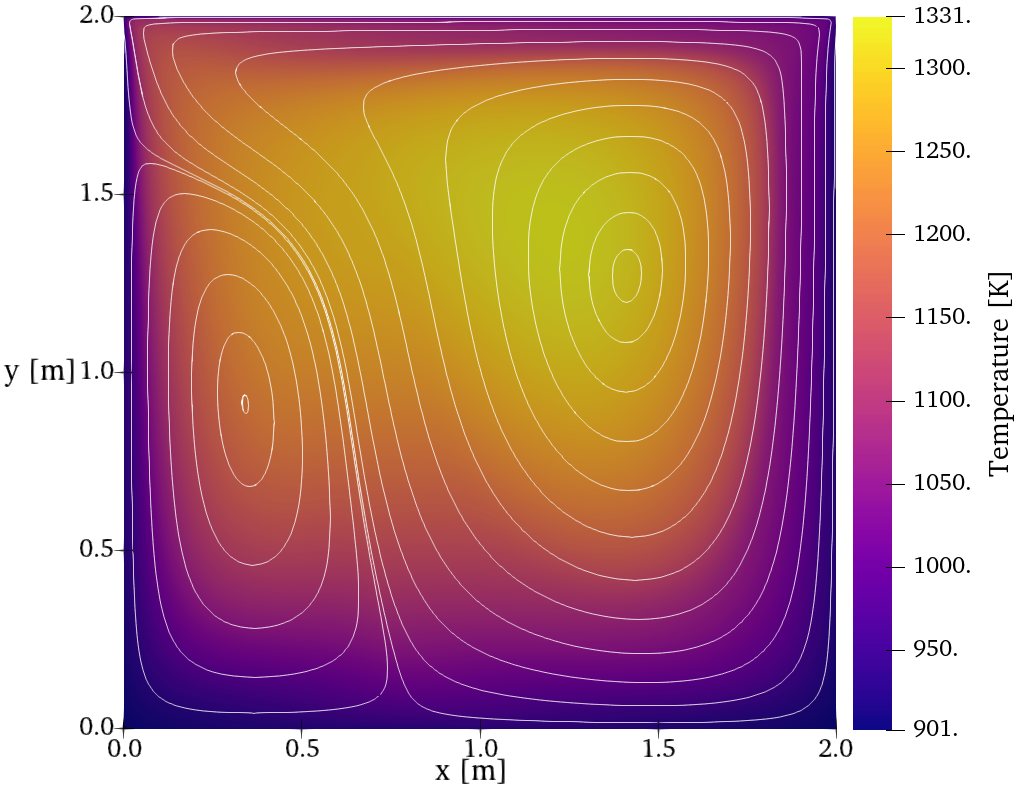
\includegraphics[width=.9\columnwidth]{full-coupled}
  \caption{Temperature distribution from Moltres for the fully coupled
  system (Step 1.4) with buoyancy effects, $P = 1$ GW, and $U_{lid} = 0.5$
  m$\cdot$s$^{-1}$. The lines correspond to the streamlines of the velocity
  field.}
  \label{fig:cnrs-color}
\end{figure}
%
\begin{table}[htb]
	\caption{Reactivity change in Step 1.4, relative to Step 0.2 under various
	$U_{lid}$ and $P$ values.}
	\centering
	\small
	\setlength\tabcolsep{1.5pt}
	\begin{tabular}{c c c c c c}
		\toprule
		& \multicolumn{5}{c}{$\rho_{s1.4} - \rho_{s0.2}$ [pcm]} \\
		\midrule
		{\backslashbox{$U_{lid}$ [m$\cdot$s$^{-1}$]}{$P$ [GW]}} & 0.2 & 0.4 & 0.6 & 0.8 & 1.0 \\
		\midrule
		0.0 & -263.7 & -498.3 & -730.9 & -966.7 & -1207.7 \\
		0.1 & -265.9 & -498.7 & -730.6 & -966.0 & -1206.7 \\
		0.2 & -268.1 & -498.8 & -729.4 & -963.7 & -1203.6 \\
		0.3 & -269.9 & -498.5 & -727.8 & -960.8 & -1199.5 \\
		0.4 & -271.9 & -498.5 & -726.5 & -958.3 & -1195.7 \\
		0.5 & -274.2 & -498.7 & -725.6 & -956.4 & -1192.7 \\
		\bottomrule
	\end{tabular}
	\label{table:full}
\end{table}

\FloatBarrier

\begin{table}[htb]
	\caption{Discrepancy values from Moltres alongside the average and standard
	deviation of the discrepancy values of the benchmark participants for Step
	2.1.}
	\centering
	\small
	\begin{tabular}{l l S S S}
		\toprule
		\multirow{2}{*}{\textbf{Step}} & \multirow{2}{*}{\textbf{Observable}} & {\multirow{2}{*}{\textbf{Moltres [\%]}}} & \multicolumn{2}{c}{\textbf{Benchmark [\%]}} \\
		& & & {Average} & {SD} \\
		\midrule
		\multirow{2}{*}{2.1} & Gain & 0.493 & 0.587 & 0.244 \\
		\cmidrule{2-5}
		& Phase shift & 1.741 & 2.176 & 0.554 \\
		\bottomrule
	\end{tabular}
	\label{table:disc2}
\end{table}
%
\begin{figure*}[htb]
	\centering
	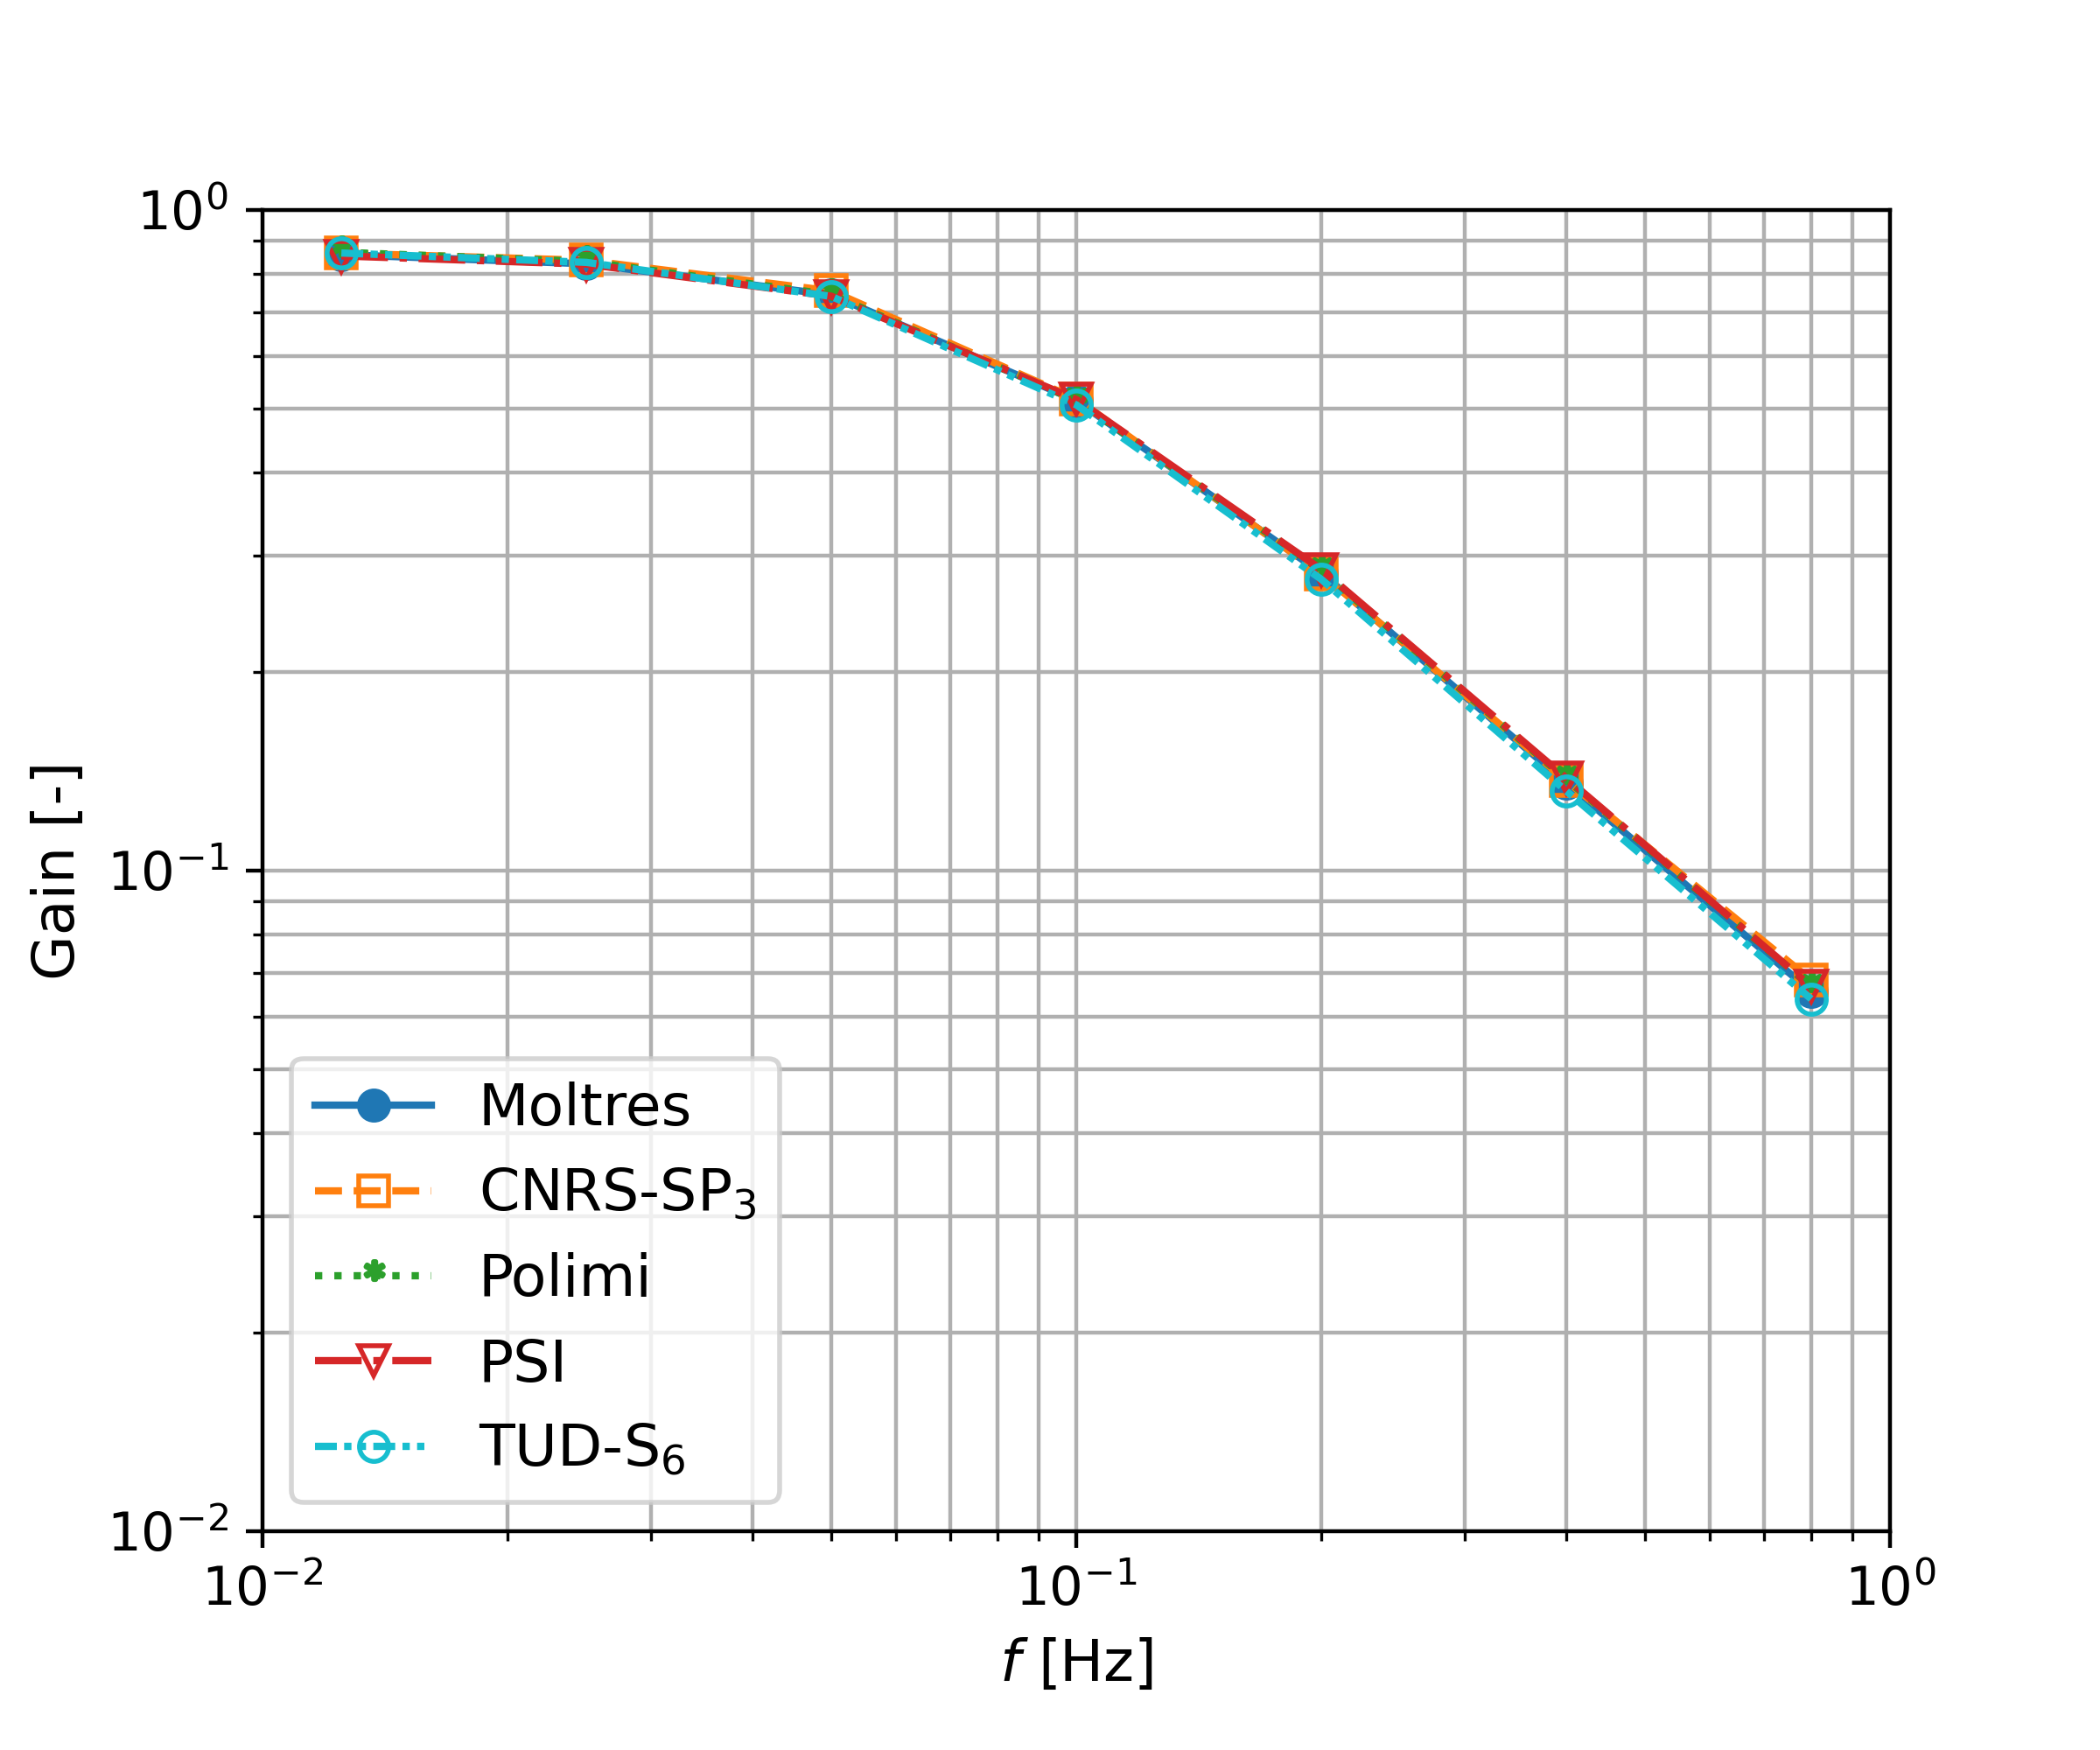
\includegraphics[width=.75\columnwidth]{2-1-gain-plot}
	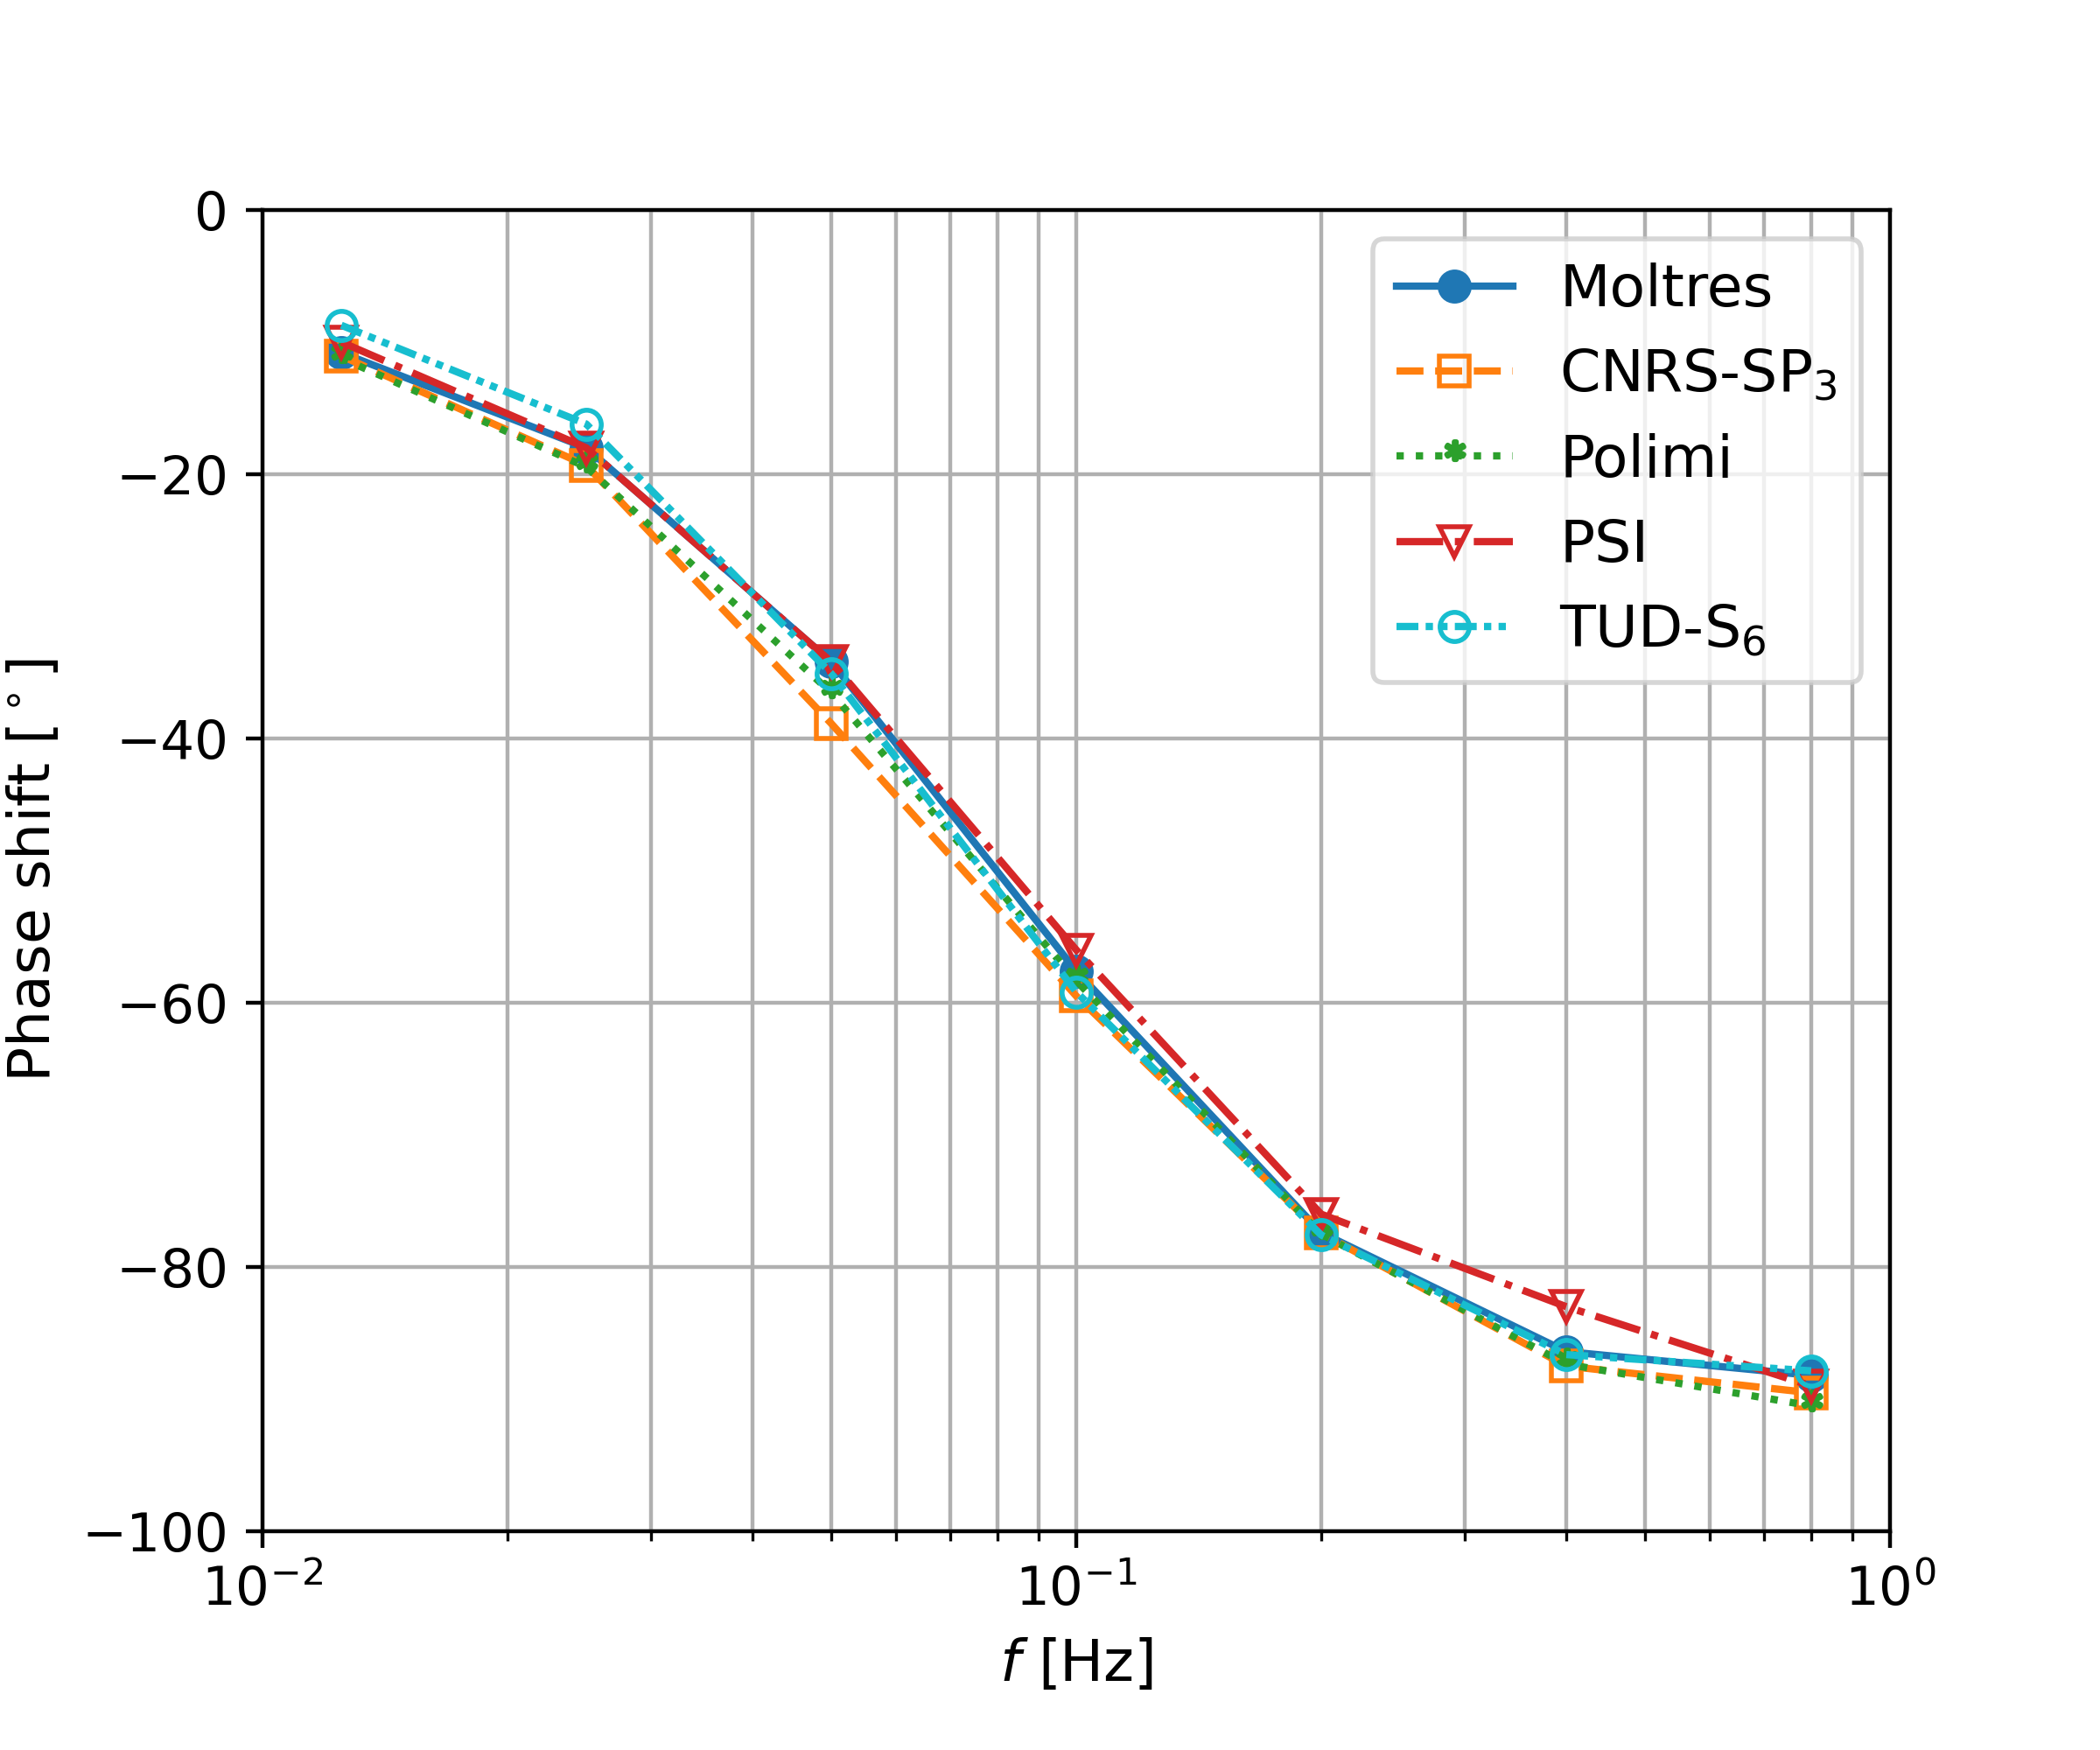
\includegraphics[width=.75\columnwidth]{2-1-phase-plot}
	\caption{Step 2.1 \textemdash\ Bode gain and phase plots of the frequency response of
	the fully coupled system.}
	\label{fig:2.1}
\end{figure*}

\subsection{Phase 2 results \& discussion}

Lastly, the following subsection discusses the results for the transient cases
in Step 2.1 which involve measuring the response in power output to periodic
perturbations in the heat transfer coefficient.

\subsubsection{Step 2.1: Forced convection transient}

Figure \ref{fig:2.1} shows the Bode gain and phase shift plots of the response
in power output in the fully coupled system. Along with the average discrepancy
values from Table \ref{table:disc2}, the results show that Moltres is
consistent with the benchmark. The gain data points from all \gls{MSR} software
agree closely with one another. Moltres reports an average discrepancy value of
0.496\%, slightly lower than the benchmark average of 0.587\%. On the other
hand, the phase shift data points show greater spread over the various driving
frequencies. We note the different timestepping schemes and timestep
sizes among the different software packages which is likely responsible for
the variations in the phase shift. Even with a precision of
$\pm0.9^\circ$ for each phase shift value, Moltres accurately reproduces the
correct trend with a lower average discrepancy (1.741\%) than the benchmark
participants' average (2.176\%).

\FloatBarrier

\section{Conclusion}

\glspl{MSR} feature significant multiphysics interactions which present
computational challenges for many existing multiphysics reactor analysis
software. This chapter presents code-to-code verification of Moltres
capabilities in modeling such multiphysics phenomena in fast-spectrum
\glspl{MSR} based on the CNRS benchmark \cite{tiberga_results_2020}.
The CNRS benchmark assesses multiphysics \gls{MSR} simulation
software through several steps involving single-physics and coupled
neutronics/thermal-hydraulics problems.

The results showed that Moltres is consistent with the participating software
presented in the CNRS benchmark paper for the modeling of important phenomena
in fast-spectrum \glspl{MSR}. The percentage discrepancies in the various
neutronics, velocity, and temperature quantities mostly fall below or within
one standard deviation of the average of the benchmark participants.
Minor deviations in the temperature in Steps 0.3 and 1.2 
stem from the discontinuous velocity
boundaries on the top corners in the lid-driven cavity flow. We have shown that
these deviations are limited to the top boundary of the domain and do not
affect the rest of the physical parameters. The results from
Moltres agree closest with the TUD-S$_2$ software package, which implements the
$S_2$ discrete ordinates method for
neutron transport on a uniform structured mesh with a \gls{DFEM}-based solver.
These features make Moltres the most similar to the TUD-$S_2$ model as compared
to the other models which employ different neutron transport models,
non-uniform meshes, and/or finite volume-based solvers.

This work verifies Moltres' capabilities for future work involving modeling and
simulation of fast-spectrum \glspl{MSR}. Fast-spectrum \glspl{MSR}
under consideration for modeling with Moltres include the European \gls{MSFR}
as a continuation of work done in \cite{park_advancement_2020}, and
TerraPower's \gls{MCFR} \cite{terrapower_terrapower_2021} from publicly
available design specifications. Moltres can play an important role in
supporting further \gls{MSR} development through enabling transient accident
safety analysis and design optimization studies on an open-source platform.
An ongoing research project involves employing Moltres as a
surrogate model for machine learning-based reactor design optimization.
We note that Moltres also supports modeling solid-fueled reactors such as the
\gls{HTGR} by disabling the precursor drift functionality as demonstrated by
\cite{fairhurst-agosta_multi-physics_2020}. Future work pertaining to
further Moltres development include introducing an intermediate-fidelity
turbulence model for highly turbulent flows in \glspl{MSR}, improving
neutronics accuracy in heterogeneous geometries, and enhancing the general
computational performance of existing features.

This work verifies Moltres' capabilities for future work involving modeling and
simulation of fast-spectrum \glspl{MSR} such as the European \gls{MSFR} and
TerraPower's \gls{MCFR} \cite{terrapower_terrapower_2021}. Notably, the CNRS
benchmark does not assess modeling capabilities for complex physics phenomena
such as turbulent flow in \glspl{MSR}. This works in favor of existing
capabilities in Moltres since Moltres doesn't currently support turbulence
modeling. However, we expect coolant loops in many \gls{MSR} designs will
experience turbulent flow under normal operation or accident scenarios.
These expectations, alongside the subpar results of pump-initiated accidents
reported in Section \ref{sec:msfr}, call for the implementation and
verification of a turbulence model in Moltres for accurate modeling of
\glspl{MSR}.

\FloatBarrier

\begin{subappendices}
    %\appendix
\section{Additional data tables} \label{appendix:tables}

This Appendix presents observable values measured at nine
equidistant points along the centerlines AA' and BB' from Moltres and the
CNRS benchmark participants \cite{tiberga_results_2020}. We refer readers to
\cite{park_results_2021} and \cite{tiberga_results_2019} for the full set of
results from Moltres and the benchmark participants. 

\begin{table}[htbp!]
	\caption{Step 0.1 \textemdash\ Velocity components along centerlines AA' and BB'.}
	\centering
	\footnotesize
	\setlength\tabcolsep{1.5pt}
	\hspace*{-1cm}
	\renewcommand{\arraystretch}{.8}
	\begin{tabular}{c c c c c c c c c c c}
		\toprule
		\multirow{2}{*}{\textbf{Observable}} & \multirow{2}{*}{\textbf{Code}} & \multicolumn{9}{c}{\textbf{Results along $AA'$} (point coordinates are expressed in m)} \\
		& & {(0,1)} & {(0.25,1)} & {(0.5,1)} & {(0.75,1)} & {(1,1)} & {(1.25,1)} & {(1.5,1)} & {(1.75,1)} & {(2,1)} \\
		\midrule
		\multirow{5}{*}{$u_x$ (m s$^{-1}$)} & Moltres & 0.000E+00 & -1.923E-02 & -5.372E-02 & -8.371E-02 & -1.025E-01 & -1.043E-01 & -7.975E-02 & -3.080E-02 & 0.000E+00 \\
		& CNRS & 0.000E+00 & -1.924E-02 & -5.372E-02 & -8.369E-02 & -1.025E-01 & -1.043E-01 & -7.972E-02 & -3.080E-02 & 0.000E+00 \\
        & PoliMi & 0.000E+00 & -1.922E-02 & -5.365E-02 & -8.357E-02 & -1.023E-01 & -1.041E-01 & -7.947E-02 & -3.066E-02 & 0.000E+00 \\
        & PSI & 0.000E+00 & -1.929E-02 & -5.366E-02 & -8.332E-02 & -1.018E-01 & -1.034E-01 & -7.912E-02 & -3.072E-02 & 0.000E+00 \\
        & TUD & 1.002E-06 & -1.922E-02 & -5.372E-02 & -8.371E-02 & -1.025E-01 & -1.044E-01 & -7.977E-02 & -3.081E-02 & 4.198E-06 \\
        \midrule
		\multirow{5}{*}{$u_y$ (m s$^{-1}$)} & Moltres & 0.000E+00 & 7.269E-02 & 8.579E-02 & 6.087E-02 & 1.250E-02 & -4.794E-02 & -9.612E-02 & -8.722E-02 & 0.000E+00\\
		& CNRS & 0.000E+00 & 7.266E-02 & 8.575E-02 & 6.084E-02 & 1.251E-02 & -4.789E-02 & -9.606E-02 & -8.722E-02 & 0.000E+00 \\
        & PoliMi & 0.000E+00 & 7.139E-02 & 8.433E-02 & 6.007E-02 & 1.269E-02 & -4.691E-02 & -9.472E-02 & -8.621E-02 & 0.000E+00 \\
        & PSI & 0.000E+00 & 7.265E-02 & 8.534E-02 & 6.021E-02 & 1.230E-02 & -4.734E-02 & -9.536E-02 & -8.720E-02 & 0.000E+00 \\
        & TUD & 5.877E-06 & 7.269E-02 & 8.580E-02 & 6.089E-02 & 1.252E-02 & -4.794E-02 & -9.613E-02 & -8.726E-02 & -1.013E-05 \\
		\midrule
		\midrule
		\multirow{2}{*}{\textbf{Observable}} & \multirow{2}{*}{\textbf{Code}} & \multicolumn{9}{c}{\textbf{Results along $BB'$} (point coordinates are expressed in m)} \\
		& & {(1,0)} & {(1,0.25)} & {(1,0.5)} & {(1,0.75)} & {(1,1)} & {(1,1.25)} & {(1,1.5)} & {(1,1.75)} & {(1,2)} \\
		\midrule
		\multirow{5}{*}{$u_x$ (m s$^{-1}$)} & Moltres & 0.000E+00 & -3.518E-02 & -6.243E-02 & -8.723E-02 & -1.025E-01 & -8.770E-02 & -1.146E-02 & 1.718E-01 & 5.000E-01 \\
		& CNRS & 0.000E+00 & -3.517E-02 & -6.242E-02 & -8.720E-02 & -1.025E-01 & -8.766E-02 & -1.147E-02 & 1.717E-01 & 5.000E-01 \\
        & PoliMi & 0.000E+00 & -3.423E-02 & -6.107E-02 & -8.613E-02 & -1.023E-01 & -8.861E-02 & -1.299E-02 & 1.706E-01 & 5.000E-01 \\
        & PSI & 0.000E+00 & -3.511E-02 & -6.217E-02 & -8.667E-02 & -1.018E-01 & -8.731E-02 & -1.191E-02 & 1.705E-01 & 5.000E-01 \\
        & TUD & 1.494E-06 & -3.519E-02 & -6.244E-02 & -8.724E-02 & -1.025E-01 & -8.770E-02 & -1.146E-02 & 1.718E-01 & 5.000E-01 \\
        \midrule
		\multirow{5}{*}{$u_y$ (m s$^{-1}$)} & Moltres & 0.000E+00 & 5.161E-05 & 6.166E-04 & 3.842E-03 & 1.250E-02 & 2.525E-02 & 3.050E-02 & 1.501E-02 & 0.000E+00 \\
		& CNRS & 0.000E+00 & 5.641E-05 & 6.309E-04 & 3.862E-03 & 1.251E-02 & 2.524E-02 & 3.048E-02 & 1.500E-02 & 0.000E+00 \\
        & PoliMi & 0.000E+00 & 9.118E-05 & 7.484E-04 & 4.046E-03 & 1.269E-02 & 2.534E-02 & 3.050E-02 & 1.500E-02 & 0.000E+00 \\
        & PSI & 0.000E+00 & 7.727E-05 & 6.822E-04 & 3.875E-03 & 1.230E-02 & 2.472E-02 & 2.994E-02 & 1.481E-02 & 0.000E+00 \\
        & TUD & 1.501E-06 & 5.260E-05 & 6.209E-04 & 3.853E-03 & 1.252E-02 & 2.528E-02 & 3.053E-02 & 1.502E-02 & 7.987E-06 \\
		\bottomrule
	\end{tabular}
\end{table}

\begin{table}[htbp!]
	\caption{Step 0.2 \textemdash\ Fission rate density along $AA'$.}
	\centering
	\footnotesize
	\setlength\tabcolsep{1.5pt}
	\hspace*{-1cm}
	\renewcommand{\arraystretch}{.8}
	\begin{tabular}{c c c c c c c c c c c}
		\toprule
		\multirow{2}{*}{\textbf{Observable}} & \multirow{2}{*}{\textbf{Code}} & \multicolumn{9}{c}{\textbf{Results along $AA'$} (point coordinates are expressed in m)} \\
		& & {(0,1)} & {(0.25,1)} & {(0.5,1)} & {(0.75,1)} & {(1,1)} & {(1.25,1)} & {(1.5,1)} & {(1.75,1)} & {(2,1)} \\
		\midrule
		\multirow{7}{*}{\shortstack[1]{$\int_E \Sigma_f \Phi$d$E$\\(m$^{-3}$s$^{-1}$)}} & Moltres & 7.701E+17 & 7.461E+18
		& 1.303E+19 & 1.672E+19 & 1.801E+19 & 1.672E+19 & 1.303E+19 &
		7.461E+18 & 7.701E+17 \\
		& CNRS-$SP_1$ & 6.896E+17 & 7.436E+18 & 1.305E+19 & 1.678E+19 & 1.809E+19 & 1.678E+19 & 1.305E+19 & 7.436E+18 & 6.896E+17 \\
		& CNRS-$SP_3$ & 6.206E+17 & 7.450E+18 & 1.303E+19 & 1.673E+19 & 1.802E+19 & 1.673E+19 & 1.303E+19 & 7.450E+18 & 6.206E+17 \\
		& PoliMi & 7.780E+17 & 7.470E+18 & 1.310E+19 & 1.684E+19 & 1.815E+19 & 1.684E+19 & 1.310E+19 & 7.470E+18 & 7.780E+17 \\
		& PSI & 8.622E+17 & 7.436E+18 & 1.305E+19 & 1.678E+19 & 1.809E+19 & 1.678E+19 & 1.305E+19 & 7.436E+18 & 8.622E+17 \\
		& TUD-$S_2$ & 6.626E+17 & 7.433E+18 & 1.307E+19 & 1.682E+19 & 1.814E+19 & 1.682E+19 & 1.307E+19 & 7.433E+18 & 6.626E+17 \\
		& TUD-$S_6$ & 6.833E+17 & 7.463E+18 & 1.300E+19 & 1.667E+19 & 1.796E+19 & 1.667E+19 & 1.300E+19 & 7.463E+18 & 6.833E+17 \\
		\bottomrule
	\end{tabular}
\end{table}

\begin{table}[htbp!]
	\caption{Step 0.3 \textemdash\ Temperature distribution along centerlines $AA'$ and $BB'$.}
	\label{table:0.3}
	\centering
	\footnotesize
	\setlength\tabcolsep{1.5pt}
	\hspace*{-1cm}
	\renewcommand{\arraystretch}{.8}
	\begin{tabular}{c c c c c c c c c c c}
		\toprule
		\multirow{2}{*}{\textbf{Observable}} & \multirow{2}{*}{\textbf{Code}} & \multicolumn{9}{c}{\textbf{Results along $AA'$} (point coordinates are expressed in m)} \\
		& & {(0,1)} & {(0.25,1)} & {(0.5,1)} & {(0.75,1)} & {(1,1)} & {(1.25,1)} & {(1.5,1)} & {(1.75,1)} & {(2,1)} \\
		\midrule
		\multirow{7}{*}{$T$ (K)} & Moltres & 9.251E+02 & 1.194E+03 & 1.357E+03 & 1.361E+03 &
		1.303E+03 & 1.224E+03 & 1.131E+03 & 1.035E+03 & 9.251E+02 \\
		& CNRS-$SP_1$ & 9.253E+02 & 1.194E+03 & 1.358E+03 & 1.363E+03 & 1.305E+03 & 1.224E+03 & 1.131E+03 & 1.034E+03 & 9.251E+02 \\
		& CNRS-$SP_3$ & 9.236E+02 & 1.194E+03 & 1.357E+03 & 1.361E+03 & 1.304E+03 & 1.224E+03 & 1.131E+03 & 1.034E+03 & 9.235E+02 \\
		& PoliMi & 9.253E+02 & 1.196E+03 & 1.361E+03 & 1.364E+03 & 1.305E+03 & 1.224E+03 & 1.132E+03 & 1.035E+03 & 9.252E+02 \\
		& PSI & 9.253E+02 & 1.196E+03 & 1.356E+03 & 1.363E+03 & 1.306E+03 & 1.226E+03 & 1.133E+03 & 1.037E+03 & 9.252E+02 \\
		& TUD-$S_2$ & 9.212E+02 & 1.194E+03 & 1.359E+03 & 1.364E+03 & 1.305E+03 & 1.224E+03 & 1.131E+03 & 1.032E+03 & 9.225E+02 \\
		& TUD-$S_6$ & 9.219E+02 & 1.194E+03 & 1.356E+03 & 1.360E+03 & 1.303E+03 & 1.223E+03 & 1.131E+03 & 1.034E+03 & 9.233E+02 \\
		\midrule
		\midrule
		\multirow{2}{*}{\textbf{Observable}} & \multirow{2}{*}{\textbf{Code}} & \multicolumn{9}{c}{\textbf{Results along $BB'$} (point coordinates are expressed in m)} \\
		& & {(1,0)} & {(1,0.25)} & {(1,0.5)} & {(1,0.75)} & {(1,1)} & {(1,1.25)} & {(1,1.5)} & {(1,1.75)} & {(1,2)} \\
		\midrule
		\multirow{7}{*}{$T$ (K)} & Moltres & 9.251E+02 & 1.140E+03 & 1.272E+03 & 1.303E+03 &
		1.303E+03 & 1.313E+03 & 1.320E+03 & 1.264E+03 & 9.123E+02 \\
		& CNRS-$SP_1$ & 9.252E+02 & 1.139E+03 & 1.273E+03 & 1.305E+03 & 1.305E+03 & 1.314E+03 & 1.321E+03 & 1.265E+03 & 9.322E+02 \\
		& CNRS-$SP_3$ & 9.236E+02 & 1.140E+03 & 1.272E+03 & 1.304E+03 & 1.304E+03 & 1.313E+03 & 1.320E+03 & 1.265E+03 & 9.322E+02 \\
		& PoliMi & 9.253E+02 & 1.140E+03 & 1.275E+03 & 1.307E+03 & 1.305E+03 & 1.313E+03 & 1.321E+03 & 1.265E+03 & 9.303E+02 \\
		& PSI & 9.252E+02 & 1.139E+03 & 1.273E+03 & 1.307E+03 & 1.306E+03 & 1.312E+03 & 1.319E+03 & 1.263E+03 & 9.481E+02 \\
		& TUD-$S_2$ & 9.215E+02 & 1.139E+03 & 1.273E+03 & 1.305E+03 & 1.305E+03 & 1.315E+03 & 1.322E+03 & 1.265E+03 & 9.374E+02 \\
		& TUD-$S_6$ & 9.222E+02 & 1.140E+03 & 1.272E+03 & 1.303E+03 & 1.303E+03 & 1.312E+03 & 1.319E+03 & 1.264E+03 & 9.390E+02 \\
		\bottomrule
	\end{tabular}
\end{table}

\begin{table}[htbp!]
	\caption{Step 1.1 \textemdash\ Delayed neutron source along centerlines $AA'$ and $BB'$.}
	\centering
	\footnotesize
	\setlength\tabcolsep{1.5pt}
	\hspace*{-1cm}
	\renewcommand{\arraystretch}{.8}
	\begin{tabular}{c c c c c c c c c c c}
		\toprule
		\multirow{2}{*}{\textbf{Observable}} & \multirow{2}{*}{\textbf{Code}} & \multicolumn{9}{c}{\textbf{Results along $AA'$} (point coordinates are expressed in m)} \\
		& & {(0,1)} & {(0.25,1)} & {(0.5,1)} & {(0.75,1)} & {(1,1)} & {(1.25,1)} & {(1.5,1)} & {(1.75,1)} & {(2,1)} \\
		\midrule
		\multirow{7}{*}{\shortstack[1]{$\sum_i \lambda_i C_i$\\(m$^{-3}$s$^{-1}$)}} & Moltres & 1.338E+16 & 1.456E+17 & 2.213E+17 & 2.412E+17 & 2.268E+17 & 1.923E+17 & 1.463E+17 & 9.273E+16 & 1.196E+16 \\
		& CNRS-$SP_1$ & 1.335E+16 & 1.452E+17 & 2.212E+17 & 2.411E+17 & 2.268E+17 & 1.923E+17 & 1.461E+17 & 9.214E+16 & 1.316E+16 \\
		& CNRS-$SP_3$ & 1.251E+16 & 1.454E+17 & 2.209E+17 & 2.406E+17 & 2.264E+17 & 1.921E+17 & 1.462E+17 & 9.245E+16 & 1.233E+16 \\
		& PoliMi & 1.321E+16 & 1.450E+17 & 2.219E+17 & 2.414E+17 & 2.266E+17 & 1.920E+17 & 1.459E+17 & 9.188E+16 & 1.292E+16 \\
		& PSI & 1.325E+16 & 1.453E+17 & 2.214E+17 & 2.413E+17 & 2.270E+17 & 1.925E+17 & 1.463E+17 & 9.218E+16 & 1.314E+16 \\
		& TUD-$S_2$ & 1.093E+16 & 1.438E+17 & 2.228E+17 & 2.426E+17 & 2.278E+17 & 1.927E+17 & 1.464E+17 & 8.968E+16 & 1.184E+16 \\
		& TUD-$S_6$ & 1.132E+16 & 1.437E+17 & 2.212E+17 & 2.405E+17 & 2.261E+17 & 1.916E+17 & 1.461E+17 & 9.029E+16 & 1.224E+16 \\
		\midrule
		\midrule
		\multirow{2}{*}{\textbf{Observable}} & \multirow{2}{*}{\textbf{Code}} & \multicolumn{9}{c}{\textbf{Results along $BB'$} (point coordinates are expressed in m)} \\
		& & {(1,0)} & {(1,0.25)} & {(1,0.5)} & {(1,0.75)} & {(1,1)} & {(1,1.25)} & {(1,1.5)} & {(1,1.75)} & {(1,2)} \\
		\midrule
		\multirow{7}{*}{\shortstack[1]{$\sum_i \lambda_i C_i$\\(m$^{-3}$s$^{-1}$)}} & Moltres & 1.296E+16 & 1.199E+17 & 1.881E+17 & 2.191E+17 & 2.268E+17 & 2.264E+17 & 2.183E+17 & 1.760E+17 & 2.827E+16 \\
		& CNRS-$SP_1$ & 1.306E+16 & 1.190E+17 & 1.881E+17 & 2.193E+17 & 2.268E+17 & 2.261E+17 & 2.178E+17 & 1.754E+17 & 3.079E+16 \\
		& CNRS-$SP_3$ & 1.222E+16 & 1.193E+17 & 1.879E+17 & 2.189E+17 & 2.264E+17 & 2.257E+17 & 2.175E+17 & 1.753E+17 & 3.072E+16 \\
		& PoliMi & 1.297E+16 & 1.186E+17 & 1.881E+17 & 2.194E+17 & 2.266E+17 & 2.260E+17 & 2.177E+17 & 1.756E+17 & 2.805E+16 \\
		& PSI & 1.299E+16 & 1.189E+17 & 1.881E+17 & 2.195E+17 & 2.270E+17 & 2.261E+17 & 2.176E+17 & 1.752E+17 & 2.730E+16 \\
		& TUD-$S_2$ & 1.109E+16 & 1.174E+17 & 1.882E+17 & 2.203E+17 & 2.278E+17 & 2.281E+17 & 2.193E+17 & 1.768E+17 & 2.655E+16 \\
		& TUD-$S_6$ & 1.143E+16 & 1.178E+17 & 1.872E+17 & 2.186E+17 & 2.261E+17 & 2.264E+17 & 2.179E+17 & 1.761E+17 & 2.728E+16 \\
		\bottomrule
	\end{tabular}
\end{table}

\begin{table}[htbp!]
	\caption{Step 1.2 \textemdash\ Temperature distribution and change in fission rate density relative to Step 0.2 along centerlines $AA'$ and $BB'$.}
	\centering
	\footnotesize
	\setlength\tabcolsep{1.5pt}
	\hspace*{-2cm}
	\renewcommand{\arraystretch}{.8}
	\begin{tabular}{c c c c c c c c c c c}
		\toprule
		\multirow{2}{*}{\textbf{Observable}} & \multirow{2}{*}{\textbf{Code}} & \multicolumn{9}{c}{\textbf{Results along $AA'$} (point coordinates are expressed in m)} \\
		& & {(0,1)} & {(0.25,1)} & {(0.5,1)} & {(0.75,1)} & {(1,1)} & {(1.25,1)} & {(1.5,1)} & {(1.75,1)} & {(2,1)} \\
		\midrule
		\multirow{7}{*}{$T$ (K)} & Moltres & 9.279E+02 & 1.196E+03 & 1.341E+03 & 1.347E+03 & 1.298E+03 & 1.225E+03 & 1.137E+03 & 1.043E+03 & 9.279E+02 \\		
		& CNRS-$SP_1$ & 9.280E+02 & 1.195E+03 & 1.341E+03 & 1.349E+03 & 1.298E+03 & 1.225E+03 & 1.136E+03 & 1.041E+03 & 9.278E+02 \\
        & CNRS-$SP_3$ & 9.262E+02 & 1.195E+03 & 1.341E+03 & 1.348E+03 & 1.298E+03 & 1.225E+03 & 1.137E+03 & 1.042E+03 & 9.260E+02 \\
        & PoliMi & 9.281E+02 & 1.198E+03 & 1.343E+03 & 1.350E+03 & 1.300E+03 & 1.226E+03 & 1.138E+03 & 1.045E+03 & 9.280E+02 \\
        & PSI & 9.282E+02 & 1.197E+03 & 1.340E+03 & 1.349E+03 & 1.300E+03 & 1.227E+03 & 1.139E+03 & 1.045E+03 & 9.280E+02 \\
        & TUD-$S_2$ & 9.235E+02 & 1.196E+03 & 1.343E+03 & 1.350E+03 & 1.300E+03 & 1.226E+03 & 1.137E+03 & 1.041E+03 & 9.250E+02 \\
        & TUD-$S_6$ & 9.243E+02 & 1.196E+03 & 1.340E+03 & 1.347E+03 & 1.298E+03 & 1.225E+03 & 1.137E+03 & 1.042E+03 & 9.258E+02 \\
        \midrule
		\multirow{7}{*}{\shortstack{$\sum^6_g \Sigma_{f,g} \phi_g(\vec{r}) -$
		\\
            $\left[\sum^6_g \Sigma_{f,g} \phi_g(\vec{r})\right]_{s_{0.2}}$ \\ (m s$^{-1}$)}} & Moltres & 8.640E+16 & 1.148E+17 & -5.668E+17 & -9.410E+17 & -7.942E+17 & -2.895E+17 & 2.540E+17 & 4.549E+17 & 8.604E+16\\
		& CNRS-$SP_1$ & 7.800E+16 & 1.169E+17 & -5.694E+17 & -9.490E+17 & -7.979E+17 & -2.853E+17 & 2.626E+17 & 4.611E+17 & 7.776E+16 \\
        & CNRS-$SP_3$ & 7.016E+16 & 1.156E+17 & -5.668E+17 & -9.427E+17 & -7.941E+17 & -2.869E+17 & 2.575E+17 & 4.578E+17 & 6.993E+16 \\
        & PoliMi & 7.556E+16 & 1.141E+17 & -5.682E+17 & -9.440E+17 & -7.906E+17 & -2.800E+17 & 2.628E+17 & 4.563E+17 & 7.522E+16 \\
        & PSI & 2.188E+15 & 1.226E+17 & -5.486E+17 & -9.275E+17 & -7.807E+17 & -2.725E+17 & 2.702E+17 & 4.632E+17 & 1.835E+15 \\
        & TUD-$S_2$ & 7.203E+16 & 1.069E+17 & -5.648E+17 & -9.534E+17 & -8.186E+17 & -2.724E+17 & 2.628E+17 & 4.531E+17 & 7.194E+16 \\
        & TUD-$S_6$ & 7.304E+16 & 1.041E+17 & -5.572E+17 & -9.382E+17 & -8.098E+17 & -2.791E+17 & 2.466E+17 & 4.431E+17 & 7.274E+16 \\
		\midrule
		\midrule
		\multirow{2}{*}{\textbf{Observable}} & \multirow{2}{*}{\textbf{Code}} & \multicolumn{9}{c}{\textbf{Results along $BB'$} (point coordinates are expressed in m)} \\
		& & {(1,0)} & {(1,0.25)} & {(1,0.5)} & {(1,0.75)} & {(1,1)} & {(1,1.25)} & {(1,1.5)} & {(1,1.75)} & {(1,2)} \\
		\midrule
		\multirow{7}{*}{$T$ (K)} & Moltres & 9.280E+02 & 1.149E+03 & 1.272E+03 & 1.300E+03 & 1.298E+03 & 1.304E+03 & 1.307E+03 & 1.253E+03 & 9.147E+02 \\		
		& CNRS-$SP_1$ & 9.281E+02 & 1.148E+03 & 1.272E+03 & 1.301E+03 & 1.298E+03 & 1.304E+03 & 1.307E+03 & 1.253E+03 & 9.350E+02 \\
        & CNRS-$SP_3$ & 9.262E+02 & 1.149E+03 & 1.272E+03 & 1.300E+03 & 1.298E+03 & 1.303E+03 & 1.306E+03 & 1.253E+03 & 9.351E+02 \\
        & PoliMi & 9.281E+02 & 1.150E+03 & 1.275E+03 & 1.304E+03 & 1.300E+03 & 1.304E+03 & 1.307E+03 & 1.253E+03 & 9.470E+02 \\
        & PSI & 9.282E+02 & 1.148E+03 & 1.273E+03 & 1.303E+03 & 1.300E+03 & 1.303E+03 & 1.306E+03 & 1.252E+03 & 9.517E+02 \\
        & TUD-$S_2$ & 9.240E+02 & 1.148E+03 & 1.274E+03 & 1.302E+03 & 1.300E+03 & 1.306E+03 & 1.309E+03 & 1.254E+03 & 9.424E+02 \\
        & TUD-$S_6$ & 9.247E+02 & 1.149E+03 & 1.272E+03 & 1.300E+03 & 1.298E+03 & 1.303E+03 & 1.306E+03 & 1.253E+03 & 9.442E+02 \\
        \midrule
		\multirow{7}{*}{\shortstack{$\sum^6_g \Sigma_{f,g} \phi_g(\vec{r}) -$
		\\
            $\left[\sum^6_g \Sigma_{f,g} \phi_g(\vec{r})\right]_{s_{0.2}}$ \\ (m s$^{-1}$)}} & Moltres & 9.077E+16 & 2.601E+17 & -2.295E+17 & -6.406E+17 & -7.942E+17 & -7.522E+17 & -4.901E+17 & -3.940E+16 & 9.584E+16\\
		& CNRS-$SP_1$ & 8.205E+16 & 2.640E+17 & -2.264E+17 & -6.431E+17 & -7.979E+17 & -7.557E+17 & -4.923E+17 & -3.953E+16 & 8.353E+16 \\
        & CNRS-$SP_3$ & 7.377E+16 & 2.615E+17 & -2.273E+17 & -6.407E+17 & -7.941E+17 & -7.525E+17 & -4.902E+17 & -3.919E+16 & 7.493E+16 \\
        & PoliMi & 7.961E+16 & 2.639E+17 & -2.256E+17 & -6.389E+17 & -7.942E+17 & -7.536E+17 & -4.922E+17 & -4.164E+16 & 8.050E+16 \\
        & PSI & 9.174E+16 & 2.639E+17 & -2.287E+17 & -6.506E+17 & -8.020E+17 & -7.479E+17 & -4.856E+17 & -3.479E+16 & 9.059E+16 \\
        & TUD-$S_2$ & 7.595E+16 & 2.513E+17 & -2.336E+17 & -6.589E+17 & -8.186E+17 & -7.703E+17 & -4.964E+17 & -4.656E+16 & 6.931E+16 \\
        & TUD-$S_6$ & 7.677E+16 & 2.436E+17 & -2.373E+17 & -6.540E+17 & -8.098E+17 & -7.612E+17 & -4.906E+17 & -4.534E+16 & 6.990E+16 \\
		\bottomrule
	\end{tabular}
\end{table}

\begin{table}[htbp!]
	\caption{Step 1.3 \textemdash\ Velocity components, temperature distribution, and delayed neutron source along centerlines $AA'$ and $BB'$.}
	\centering
	\footnotesize
	\setlength\tabcolsep{1.5pt}
	\hspace*{-1cm}
	\renewcommand{\arraystretch}{.63}
	\begin{tabular}{c c c c c c c c c c c}
        \toprule
		\multirow{2}{*}{\textbf{Observable}} & \multirow{2}{*}{\textbf{Code}} & \multicolumn{9}{c}{\textbf{Results along $AA'$} (point coordinates are expressed in m)} \\
		& & {(0,1)} & {(0.25,1)} & {(0.5,1)} & {(0.75,1)} & {(1,1)} & {(1.25,1)} & {(1.5,1)} & {(1.75,1)} & {(2,1)} \\
        \midrule
        \multirow{7}{*}{$u_x$ (m s$^{-1}$)} & Moltres    &   0.000E+00 &   1.635E+00 &   2.300E+00 &   1.570E+00 &  -1.487E-08 &  -1.570E+00 &  -2.300E+00 &  -1.635E+00 &   0.000E+00 \\
        & CNRS-$SP_1$   &   0.000E+00 &   1.641E-02 &   2.310E-02 &   1.579E-02 &   1.250E-09 &  -1.579E-02 &  -2.310E-02 &  -1.641E-02 &   0.000E+00 \\
        & CNRS-$SP_3$   &   0.000E+00 &   1.636E-02 &   2.302E-02 &   1.572E-02 &   1.000E-09 &  -1.572E-02 &  -2.302E-02 &  -1.636E-02 &   0.000E+00 \\
        & PoliMi     &   0.000E+00 &   1.637E-02 &   2.312E-02 &   1.578E-02 &  -1.125E-10 &  -1.578E-02 &  -2.312E-02 &  -1.637E-02 &   0.000E+00 \\
        & PSI        &   0.000E+00 &   1.630E-02 &   2.263E-02 &   1.519E-02 &  -8.525E-09 &  -1.519E-02 &  -2.263E-02 &  -1.630E-02 &   0.000E+00 \\
        & TUD-$S_2$     &   6.054E-06 &   1.644E-02 &   2.316E-02 &   1.584E-02 &  -2.218E-06 &  -1.584E-02 &  -2.316E-02 &  -1.644E-02 &  -6.054E-06 \\
        & TUD-$S_6$     &   5.982E-06 &   1.631E-02 &   2.295E-02 &   1.566E-02 &  -2.196E-06 &  -1.566E-02 &  -2.295E-02 &  -1.631E-02 &  -5.982E-06 \\
        \midrule
        \multirow{7}{*}{$u_y$ (m s$^{-1}$)} & Moltres    &   0.000E+00 &  -1.769E+01 &   1.698E+00 &   1.371E+01 &   1.643E+01 &   1.371E+01 &   1.698E+00 &  -1.769E+01 &   0.000E+00 \\
        & CNRS-$SP_1$   &   0.000E+00 &  -1.777E-01 &   1.721E-02 &   1.376E-01 &   1.649E-01 &   1.376E-01 &   1.721E-02 &  -1.777E-01 &   0.000E+00 \\
        & CNRS-$SP_3$   &   0.000E+00 &  -1.771E-01 &   1.708E-02 &   1.372E-01 &   1.645E-01 &   1.372E-01 &   1.708E-02 &  -1.771E-01 &   0.000E+00 \\
        & PoliMi     &   0.000E+00 &  -1.767E-01 &   1.741E-02 &   1.368E-01 &   1.638E-01 &   1.368E-01 &   1.741E-02 &  -1.767E-01 &   0.000E+00 \\
        & PSI        &   0.000E+00 &  -1.779E-01 &   1.662E-02 &   1.376E-01 &   1.659E-01 &   1.376E-01 &   1.662E-02 &  -1.779E-01 &   0.000E+00 \\
        & TUD-$S_2$     &  -2.886E-05 &  -1.780E-01 &   1.735E-02 &   1.379E-01 &   1.650E-01 &   1.379E-01 &   1.735E-02 &  -1.780E-01 &  -2.886E-05 \\
        & TUD-$S_6$     &  -2.929E-05 &  -1.766E-01 &   1.694E-02 &   1.368E-01 &   1.639E-01 &   1.368E-01 &   1.694E-02 &  -1.766E-01 &  -2.929E-05 \\
        \midrule
        \multirow{7}{*}{$T$ (K)} & Moltres  &   9.284E+02 &   1.192E+03 &   1.277E+03 &   1.284E+03 &   1.280E+03 &   1.284E+03 &   1.277E+03 &   1.192E+03 &   9.284E+02 \\
        & CNRS-$SP_1$ &   9.279E+02 &   1.193E+03 &   1.278E+03 &   1.284E+03 &   1.280E+03 &   1.284E+03 &   1.278E+03 &   1.193E+03 &   9.279E+02 \\
        & CNRS-$SP_3$ &   9.260E+02 &   1.193E+03 &   1.278E+03 &   1.284E+03 &   1.280E+03 &   1.284E+03 &   1.278E+03 &   1.193E+03 &   9.260E+02 \\
        & PoliMi   &   9.279E+02 &   1.193E+03 &   1.279E+03 &   1.286E+03 &   1.282E+03 &   1.286E+03 &   1.279E+03 &   1.193E+03 &   9.279E+02 \\
        & PSI      &   9.279E+02 &   1.191E+03 &   1.278E+03 &   1.284E+03 &   1.280E+03 &   1.284E+03 &   1.278E+03 &   1.191E+03 &   9.279E+02 \\
        & TUD-$S_2$   &   9.248E+02 &   1.193E+03 &   1.279E+03 &   1.285E+03 &   1.281E+03 &   1.285E+03 &   1.279E+03 &   1.193E+03 &   9.248E+02 \\
        & TUD-$S_6$   &   9.257E+02 &   1.192E+03 &   1.277E+03 &   1.283E+03 &   1.280E+03 &   1.283E+03 &   1.277E+03 &   1.192E+03 &   9.257E+02 \\
        \midrule
        \multirow{7}{*}{\shortstack[1]{$\sum_i \lambda_i C_i$\\(m$^{-3}$s$^{-1}$)}} & Moltres   &   1.443E+16 &   1.457E+17 &   1.984E+17 &   2.102E+17 &   1.959E+17 &   2.102E+17 &   1.984E+17 &   1.457E+17 &   1.443E+16 \\
        & CNRS-$SP_1$  &   1.499E+16 &   1.468E+17 &   2.001E+17 &   2.123E+17 &   1.988E+17 &   2.123E+17 &   2.001E+17 &   1.468E+17 &   1.499E+16 \\
        & CNRS-$SP_3$  &   1.409E+16 &   1.469E+17 &   2.000E+17 &   2.121E+17 &   1.986E+17 &   2.121E+17 &   2.000E+17 &   1.469E+17 &   1.409E+16 \\
        & PoliMi    &   1.436E+16 &   1.464E+17 &   1.992E+17 &   2.113E+17 &   1.944E+17 &   2.113E+17 &   1.992E+17 &   1.464E+17 &   1.436E+16 \\
        & PSI       &   1.477E+16 &   1.469E+17 &   2.005E+17 &   2.126E+17 &   1.983E+17 &   2.126E+17 &   2.005E+17 &   1.469E+17 &   1.477E+16 \\
        & TUD-$S_2$    &   1.041E+16 &   1.488E+17 &   2.017E+17 &   2.141E+17 &   1.942E+17 &   2.141E+17 &   2.017E+17 &   1.488E+17 &   1.041E+16 \\
        & TUD-$S_6$    &   1.086E+16 &   1.485E+17 &   2.006E+17 &   2.128E+17 &   1.931E+17 &   2.128E+17 &   2.006E+17 &   1.485E+17 &   1.086E+16 \\
        \midrule
        \midrule
        \multirow{2}{*}{\textbf{Observable}} & \multirow{2}{*}{\textbf{Code}} & \multicolumn{9}{c}{\textbf{Results along $BB'$} (point coordinates are expressed in m)} \\
		& & {(1,0)} & {(1,0.25)} & {(1,0.5)} & {(1,0.75)} & {(1,1)} & {(1,1.25)} & {(1,1.5)} & {(1,1.75)} & {(1,2)} \\
		\midrule
        \multirow{7}{*}{$u_y$ (m s$^{-1}$)} & Moltres    &   0.000E+00 &  -1.511E-07 &  -1.568E-07 &  -1.023E-07 &  -1.487E-08 &   8.013E-08 &   1.580E-07 &   1.791E-07 &   0.000E+00 \\
        & CNRS-$SP_1$   &   0.000E+00 &   3.512E-02 &   8.947E-02 &   1.359E-01 &   1.649E-01 &   1.665E-01 &   1.307E-01 &   5.756E-02 &   0.000E+00 \\
        & CNRS-$SP_3$   &   0.000E+00 &   3.510E-02 &   8.933E-02 &   1.356E-01 &   1.645E-01 &   1.660E-01 &   1.303E-01 &   5.740E-02 &   0.000E+00 \\
    & PoliMi     &   0.000E+00 &   3.507E-02 &   8.909E-02 &   1.351E-01 &   1.638E-01 &   1.656E-01 &   1.302E-01 &   5.743E-02 &   0.000E+00 \\
        & PSI        &   0.000E+00 &   3.537E-02 &   9.055E-02 &   1.374E-01 &   1.659E-01 &   1.669E-01 &   1.309E-01 &   5.780E-02 &   0.000E+00 \\
        & TUD-$S_2$     &  -1.234E-05 &   3.510E-02 &   8.950E-02 &   1.360E-01 &   1.650E-01 &   1.667E-01 &   1.308E-01 &   5.763E-02 &  -2.808E-05 \\
        & TUD-$S_6$     &  -1.327E-05 &   3.506E-02 &   8.912E-02 &   1.352E-01 &   1.639E-01 &   1.655E-01 &   1.299E-01 &   5.719E-02 &  -2.872E-05 \\
        \midrule
        \multirow{7}{*}{$T$ (K)} & Moltres  &   0.000E+00 &   3.512E+00 &   8.928E+00 &   1.355E+01 &   1.643E+01 &   1.658E+01 &   1.302E+01 &   5.734E+00 &   0.000E+00 \\
        & CNRS-$SP_1$ &   9.280E+02 &   1.067E+03 &   1.156E+03 &   1.226E+03 &   1.280E+03 &   1.315E+03 &   1.326E+03 &   1.283E+03 &   9.284E+02 \\
        & CNRS-$SP_3$ &   9.261E+02 &   1.067E+03 &   1.156E+03 &   1.226E+03 &   1.280E+03 &   1.315E+03 &   1.325E+03 &   1.282E+03 &   9.266E+02 \\
        & PoliMi   &   9.280E+02 &   1.067E+03 &   1.157E+03 &   1.228E+03 &   1.282E+03 &   1.317E+03 &   1.327E+03 &   1.284E+03 &   9.282E+02 \\
        & PSI      &   9.281E+02 &   1.068E+03 &   1.156E+03 &   1.226E+03 &   1.280E+03 &   1.314E+03 &   1.324E+03 &   1.281E+03 &   9.287E+02 \\
        & TUD-$S_2$   &   9.250E+02 &   1.066E+03 &   1.156E+03 &   1.227E+03 &   1.281E+03 &   1.316E+03 &   1.327E+03 &   1.283E+03 &   9.137E+02 \\
        & TUD-$S_6$   &   9.258E+02 &   1.069E+03 &   1.157E+03 &   1.226E+03 &   1.280E+03 &   1.314E+03 &   1.325E+03 &   1.282E+03 &   9.149E+02 \\
        \midrule
        \multirow{7}{*}{\shortstack[1]{$\sum_i \lambda_i C_i$\\(m$^{-3}$s$^{-1}$)}} & Moltres   &   9.279E+02 &   1.068E+03 &   1.156E+03 &   1.226E+03 &   1.280E+03 &   1.314E+03 &   1.325E+03 &   1.282E+03 &   9.283E+02 \\
        & CNRS-$SP_1$  &   1.479E+16 &   8.797E+16 &   1.377E+17 &   1.746E+17 &   1.988E+17 &   2.087E+17 &   2.017E+17 &   1.659E+17 &   1.721E+16 \\
        & CNRS-$SP_3$  &   1.383E+16 &   8.839E+16 &   1.378E+17 &   1.746E+17 &   1.986E+17 &   2.084E+17 &   2.015E+17 &   1.659E+17 &   1.631E+16 \\
        & PoliMi    &   1.451E+16 &   8.624E+16 &   1.344E+17 &   1.706E+17 &   1.944E+17 &   2.045E+17 &   1.977E+17 &   1.623E+17 &   1.583E+16 \\
        & PSI       &   1.477E+16 &   8.782E+16 &   1.373E+17 &   1.741E+17 &   1.983E+17 &   2.083E+17 &   2.014E+17 &   1.658E+17 &   1.689E+16 \\
        & TUD-$S_2$    &   1.337E+16 &   8.510E+16 &   1.335E+17 &   1.700E+17 &   1.942E+17 &   2.047E+17 &   1.980E+17 &   1.621E+17 &   1.243E+16 \\
        & TUD-$S_6$    &   1.378E+16 &   8.605E+16 &   1.335E+17 &   1.693E+17 &   1.931E+17 &   2.034E+17 &   1.969E+17 &   1.616E+17 &   1.300E+16 \\
        \bottomrule
    \end{tabular}
\end{table}

\end{subappendices}
\glsresetall

\chapter{Hybrid S$_\text{N}$-Diffusion Method for Improved Control Rod Modeling
in Neutron Diffusion Methods}
\label{chap:hybrid}
Section \ref{sec:summary-nts-mtds} highlighted the poor performance of neutron diffusion
methods for calculating neutron fluxes near control rods. Strong neutron absorption in the control
rod region produces highly anisotropic neutron flux extending some distance outside the control
rod. Neutron transport methods, which retain angular dependence of the neutron flux to various
extents, generally fare better than neutron diffusion methods with isotropic diffusion
coefficients. However, neutron transport methods are also generally more computationally expensive,
given the increased dimensionality of the problem from the angular component. Piling this extra
dimension on top of the existing geometric and neutron energy group dimensions dramatically
increases the number of unknowns to be solved in a system. Many past efforts have tried introducing
transport correction techniques to improve neutron flux and multiplication factor estimates in
diffusion-based methods. Other than control rod regions, these techniques may also correct
homogenization errors introduced by spatial homogenization of fuel assemblies and other
structures within a reactor core. They invariably rely on neutron transport methods to generate
transport corrections in the form of corrected diffusion coefficients
\cite{bretscher_computing_1997, scherer_determination_1976, ronen_accurate_2004,
pounders_diffusion_2009, kavenoky_sph_1978}, boundary conditions \cite{davison_influence_1951,
pellaud_extrapolation_1968, fen_modelling_1992}, Eddington factors, or discontinuity factors
\cite{koebke_new_1980}.

In this chapter, I propose a novel hybrid method for improving control rod modeling in neutron
diffusion solvers without spatial homogenization. In essence, the hybrid method involves applying
the $S_N$ discrete ordinates neutron transport method on subregions containing the control rod to
obtain diffusion coefficients which provide pointwise corrections for the diffusion method on the
entire problem domain.

Section \ref{sec:hybrid-theory} discusses the theoretical background for the Hybrid $S_N$-Diffusion
method. Section \ref{sec:implementation} provides numerical implementation details of
the hybrid method and its components. Sections \ref{sec:test-case} and \ref{sec:sim-param} describe
the 1-D test cases and several simulation parameters in that context. Section
\ref{sec:prelim-results} discusses the results of the hybrid method applied to the 1-D test cases
with comparisons to higher-fidelity Monte Carlo and $S_N$ neutron transport methods. Lastly,
Section \ref{sec:hybrid-summary} summarizes the key findings in this chapter.

\section{Theory} \label{sec:hybrid-theory}

The proposed Hybrid $S_N$-Diffusion method is a two-level, iterative method to improve the
accuracy of neutron diffusion solutions in reactor systems with highly neutron-absorbing control
rod regions. In this discussion, I focus on the 1-D, $k$-eigenvalue implementation of the
hybrid method.

The discrete ordinates ($S_N$) method for solving the multigroup neutron transport equation
(Eq. \ref{eq:mg-bte}) discretizes the continuous angular directional phase space into a finite
number of discrete angular intervals (ordinates). The set of distinct direction variables
$\hat{\Omega}_n$ representing the discrete ordinates is typically chosen in conjunction with a
compatible quadrature set to replace integrals across continuous solid angles
$\hat{\Omega}$ with quadrature approximations. The multigroup, discrete ordinates ($S_N$
approximation) form of the 1-D, $k$-eigenvalue neutron transport equation with the Gauss-Legendre
quadrature set is:
%
\begin{align}
  \mu_n \frac{d}{dx}\Psi_g(x, \mu_n) + \Sigma_{t,g}(x)&\Psi_g(x, \mu_n) -
\sum^G_{g'=1} \sum^N_{n'=1} \sum^L_{l=0} \frac{\left(2l+1\right)}{2}
\Sigma^{g'\rightarrow g}_{s,l}(x) P_l(\mu_{n'} - \mu_n)
w_{n'}\Psi_{g'}(x,\mu_{n'}) \nonumber \\
  &= \sum^G_{g'=1} \frac{\chi_g}{2} \frac{\nu\Sigma_{f,g'}(x)}{k} \phi_{g'}(x) + S_g(x,\mu_n)
  \label{eq:1d-sn}
  \shortintertext{where}
  \mu_n &= \mbox{ cosine of $\hat{\Omega}_n$ relative to the $x$-axis,} \nonumber \\
  \Psi_g(x,\mu_n) &= \mbox{ neutron angular flux along $\mu_n$ in group $g$,} \nonumber \\
%  g &= \mbox{ neutron energy group index, ranging from 1 to G,} \nonumber \\
%  \Sigma_{t,g}(x) &= \mbox{ macroscopic total cross section of neutrons in group $g$,} \nonumber \\
%  G &= \mbox{ total number of energy groups,} \nonumber \\
%  n &= \mbox{ discrete ordinate index,} \nonumber \\
%  N &= \mbox{ total number of discrete ordinates,} \nonumber \\
  l &= \mbox{ Legendre expansion order,} \nonumber \\
  L &= \mbox{ highest Legendre expansion order,} \nonumber \\
  \Sigma^{g'\rightarrow g}_{s,l}(x) &= \mbox{ $l$-th Legendre moment of the macroscopic
scattering} \nonumber \\
  &\ \ \ \ \mbox{ cross section from group $g'$ to $g$,} \nonumber \\
  P_l &= \mbox{ Legendre polynomial of degree $l$,} \nonumber \\
  w_{n'} &= \mbox{ $n'$-th quadrature weight,} \nonumber \\
%  \chi_g &= \mbox{ fission neutron spectrum in group $g$,} \nonumber \\
%  \nu &= \mbox{ neutrons produced per fission reaction,} \nonumber \\
%  \Sigma_{f,g}(x) &= \mbox{ macroscopic fission cross section of neutrons in group $g$,}
%  \nonumber \\
  k &= \mbox{ neutron multiplication factor.} \nonumber
%  \phi_{g'}(x) &= \mbox{ scalar neutron flux in group $g$,} \nonumber \\
%  S_g(x,\mu_n) &= \mbox{ external neutron source in group $g$.} \nonumber
\end{align}
%
We can retrieve the neutron scalar flux and current by calculating the 0th and 1st Legendre
moments as follows:
%
\begin{align}
  \phi_g(x) &= \frac{1}{2} \int^1_{-1} d\mu\ \Psi_g(x,\mu) = \frac{1}{2} \sum^N_{n=1} w_n
\Psi_g(x,\mu_n)
  \shortintertext{and}
  J_g(x) &= \frac{1}{2} \int^1_{-1} d\mu\ \mu\Psi_g(x,\mu) = \frac{1}{2} \sum^N_{n=1} w_n
\mu_n \Psi_g(x,\mu_n)
\end{align}

The 1-D form of the multigroup $k$-eigenvalue neutron diffusion equations (Eq. \ref{eq:mg-diff})
is:
%
\begin{align}
  -\frac{d}{dx} D_g(x) \frac{d}{dx} \phi_g(x) + \Sigma_{t,g}(x) \phi_g(x) &= \sum^G_{g'=1}\left[
  \Sigma_s^{g'\rightarrow g}(x)\phi_{g'}(x) + \chi_g\frac{\nu\Sigma_{f,g'}(x)}{k}
  \phi_{g'}(x)\right] + S_g(x)
  \label{eq:1d-diff}
  \shortintertext{where}
    D_g(x) &= \frac{1}{3 \Sigma_{tr}(x)} = \mbox{ neutron diffusion coefficient for group }g.
  \nonumber
\end{align}

\subsection{Spatially Varying Diffusion Coefficients} \label{sec:svdc}

The conventional approach for determining diffusion coefficients for each subregion involves
running a high-fidelity neutron transport to tally region-wide estimates of the neutron transport
cross section. The transport cross section formulation is derived from the $P_1$ approximation of
the neutron transport equation with isotropic sources \cite{bell_nuclear_1970}. Essentially, each
defined subregion has a constant diffusion coefficient value. However, as discussed in Section
\ref{sec:summary-nts-mtds}, the neutron diffusion
equation is only valid in regions of high scattering-to-removal ratios with, at most, linearly
anisotropic scattering and small flux gradients. These conditions do not hold in control rods, near
interfaces of neighboring materials with highly dissimilar neutronic properties, and in materials
with significant scattering contributions from light nuclei.

In the Hybrid $S_N$-Diffusion method, I propose replacing the conventional $P_1$-based
diffusion coefficients with an alternate formulation that incorporates pointwise corrections
to the neutron diffusion flux solution from the $S_N$-derived flux solution as follows:
%
\begin{align}
  D^s_g(x) &= -J^{tr}_g(x)\bigg/\frac{d\phi^{tr}_g(x)}{dx}. \label{eq:svdc}
\end{align}
%
where $D^s$ is the \glspl{SVDC}, and the $tr$ superscript denotes neutron current and scalar flux
solutions from the $S_N$ method.
The basic form of this equation is Fick's first law of diffusion. The result is a diffusion
coefficient variable that varies in space, even within a subdomain. \glspl{SVDC} provide pointwise
corrections to closely match the diffusion flux solution to the $S_N$ flux solution.

Pounders \& Rahnema \cite{pounders_diffusion_2009} demonstrated the effectiveness of applying
pointwise corrections derived from analytical or Monte Carlo reference flux solutions. Compared
with conventional $P_1$-based out-scatter and flux-limited approximations of the diffusion
coefficient, their \textit{high-order empirical diffusion coefficient} showed superior agreement
with the reference flux solutions. Their formulation for these piecewise-constant empirical
diffusion coefficients in Eq. \ref{eq:emp} is similar to the formulation for \glspl{SVDC} in Eq.
\ref{eq:svdc}. They recognized that volume averaging within each mesh element for
piecewise-constant coefficients introduces some truncation error if the flux is
non-linear within each mesh element. This design choice may be due to an intention to retain the
diffusion coefficient as a constant in the $\frac{d}{dx}D\frac{d\phi}{dx}$ term of the neutron
diffusion equation (Eq. \ref{eq:1d-diff}).

Unlike their approach, the \gls{SVDC} formulation in Eq. \ref{eq:svdc} allows for continuously
varying diffusion coefficients to reduce truncation error. In practice, the discretization order of
\gls{SVDC} variables in a numerical calculation would be the same as the discretization order of
the reference flux solution. This formulation introduces a minor change to the finite difference
implementation of the 2nd-order diffusion term to handle spatial derivatives of the
diffusion coefficient. However, the finite element implementation sees no change as the 2nd-order
diffusion term is commonly treated with integration-by-parts to reduce it to a 1st-order
differential term with no derivatives of the diffusion coefficient. Refer to Section
\ref{sec:implementation} for key numerical implementation details of a finite difference neutron
diffusion solver with support for handling \glspl{SVDC}.

\begin{figure}[htb!]
  \centering
  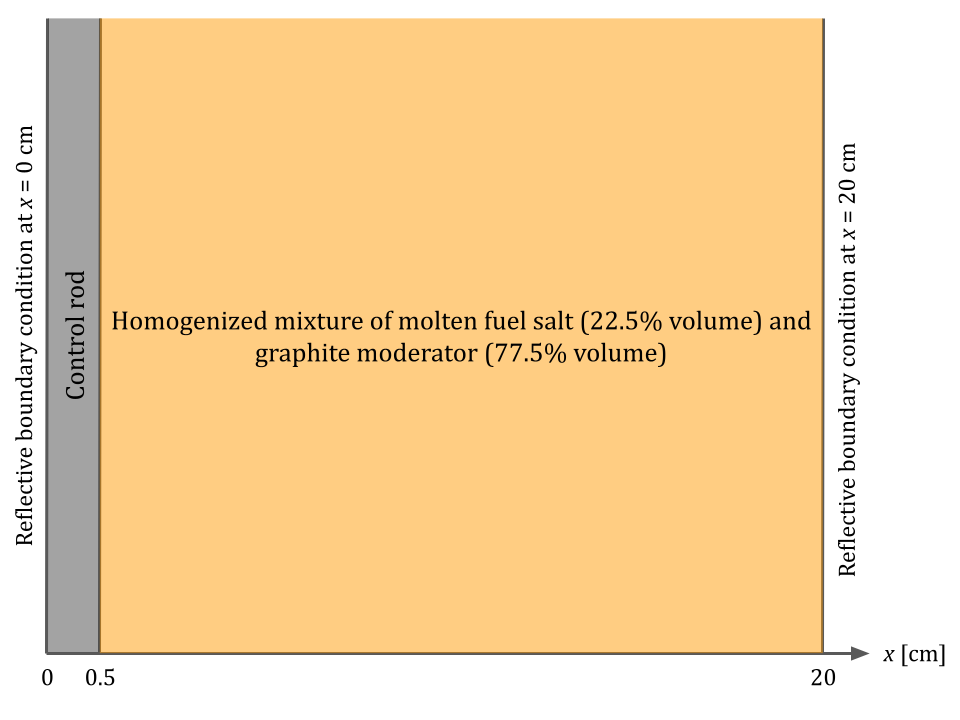
\includegraphics[width=.7\columnwidth]{case-0-geometry}
  \caption{A 1-D, two-region system containing a 0.5-cm thick control rod and a 24.5-cm thick
    homogeneous mixture of molten fuel salt and graphite moderator. Reflective boundary conditions
    apply on both ends.}
  \label{fig:case-0-geom}
\end{figure}

\subsubsection{\gls{SVDC} Verification with Case 0}

To facilitate the following demonstration of a neutron diffusion calculation with \glspl{SVDC},
consider a 1-D, two-region system (Case 0) consisting of a highly neutron-absorbing material and a
neutron-multiplying region with reflective boundary conditions on both ends (Figure
\ref{fig:case-0-geom}). I defined the material specifications of the control rod, molten fuel salt,
and graphite moderator based on the material compositions of the \gls{MSRE}
\cite{robertson_msre_1965}. The
homogenized molten fuel salt and graphite regions minimize discrepancies arising from geometrical
heterogeneity. The group constant input data for the diffusion and $S_N$ solvers (e.g., $P_1$-based
diffusion coefficients, cross
sections, fission spectra) were sampled at 900 K and generated using the OpenMC Monte Carlo
neutronics software \cite{romano_openmc:_2015}. OpenMC uses the flux-limited approximation method
to calculate diffusion coefficients \cite{pomraning_flux-limited_1984}. The condensed
neutron energy spectrum forms two discrete groups bounded at $10^{-5}$, $10^0$, and $10^8$ eV.

I solved for the neutron flux in this system using the following set of numerical solvers:
%
\begin{enumerate}
  \item Neutron diffusion solver with $P_1$-based diffusion coefficients generated directly from
    the group constant generation step with OpenMC.
  \item $S_N$ neutron transport solver with $N=8$ and up to 2nd-order Legendre
    moments of the group-to-group neutron scattering cross sections.
  \item Neutron diffusion solver with \glspl{SVDC} generated from the prior $S_8$
    flux solution.
\end{enumerate}
%
I implemented the diffusion solvers using the finite difference method and the $S_N$
solver using the diamond-difference transport sweep method in Python. For
brevity, I defer further numerical implementation details of these solvers to Section
\ref{sec:implementation}.

\begin{figure}[htb!]
  \centering
  \begin{subfigure}[b]{.49\textwidth}
    \centering
    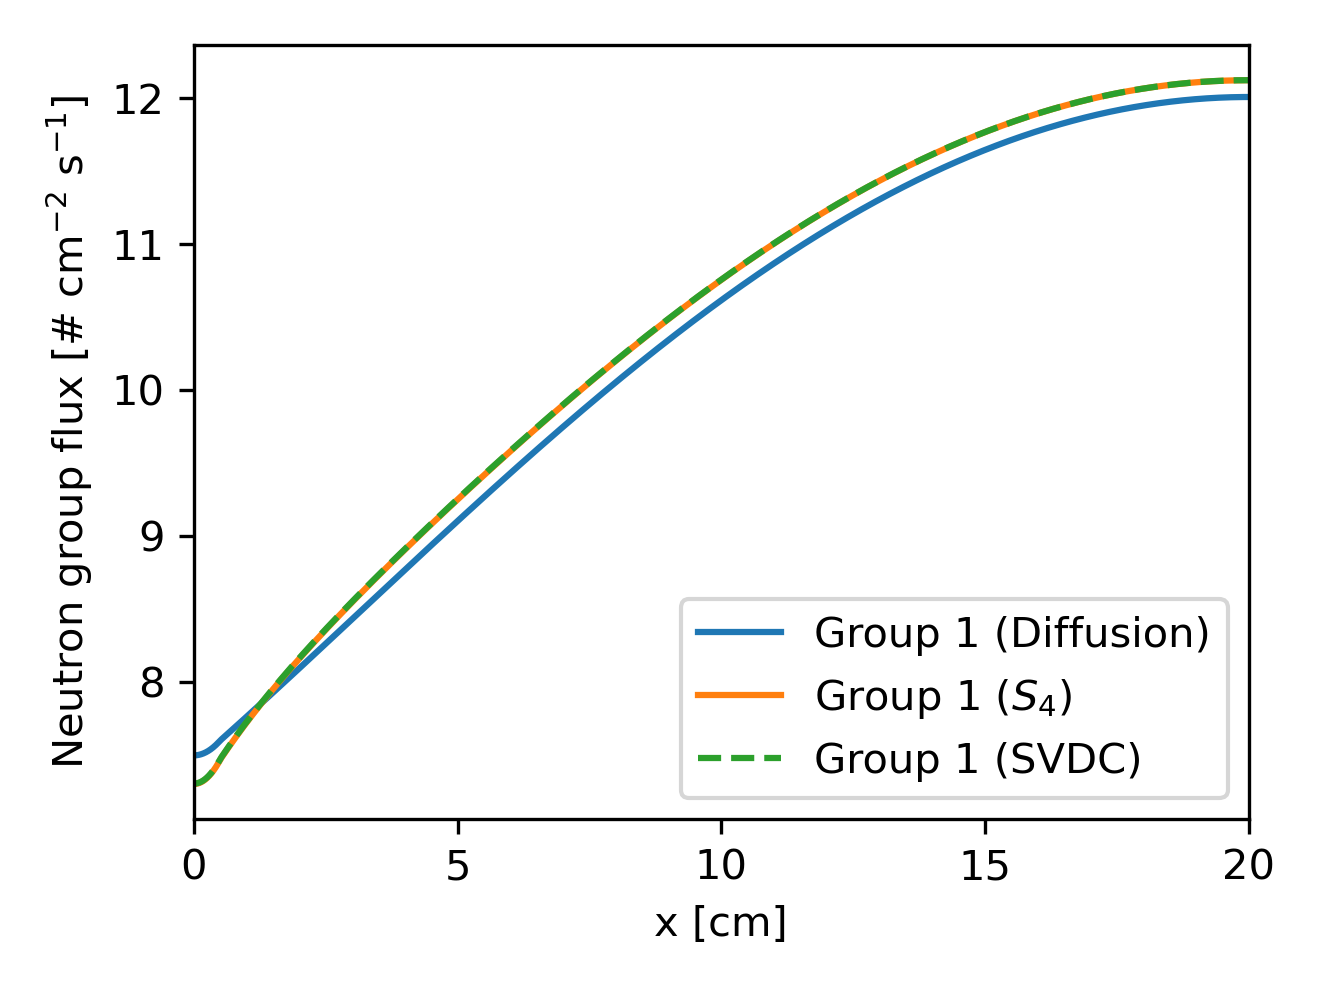
\includegraphics[width=\textwidth]{case-0-group-1-flux}
    \caption{Group 1}
    \label{fig:c0g1flux}
  \end{subfigure}
  \hfill
  \begin{subfigure}[b]{.49\textwidth}
    \centering
    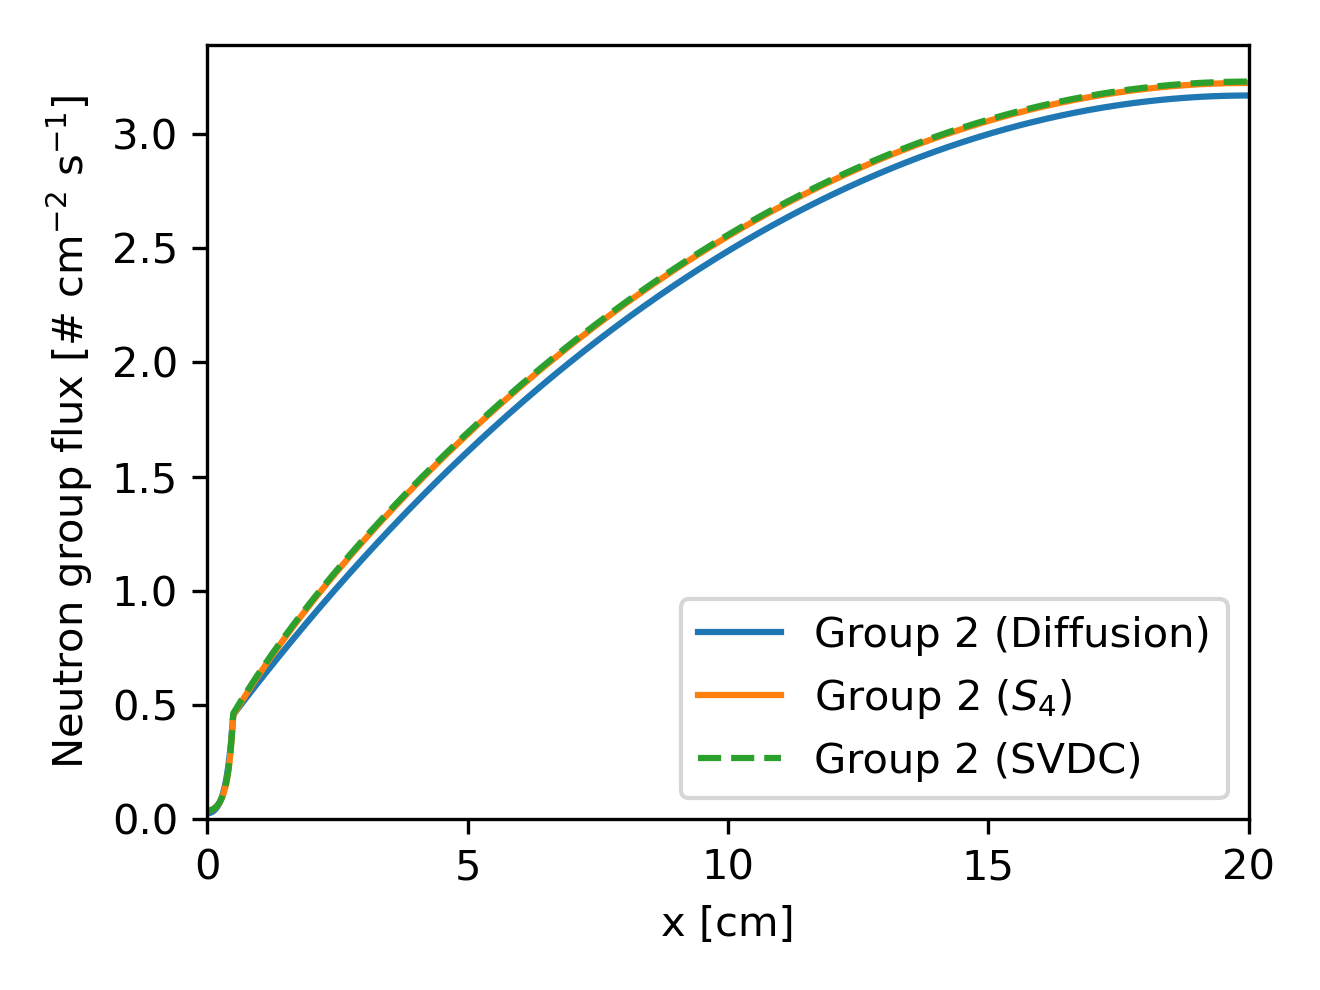
\includegraphics[width=\textwidth]{case-0-group-2-flux}
    \caption{Group 2}
    \label{fig:c0g2flux}
  \end{subfigure}
  \caption{Neutron group 1 and 2 flux distributions from the diffusion, $S_8$, and
  diffusion-\gls{SVDC} solvers for Case 0.}
  \label{fig:c0flux}
\end{figure}
%
\begin{figure}[htb!]
  \centering
  \begin{subfigure}[b]{.49\textwidth}
    \centering
    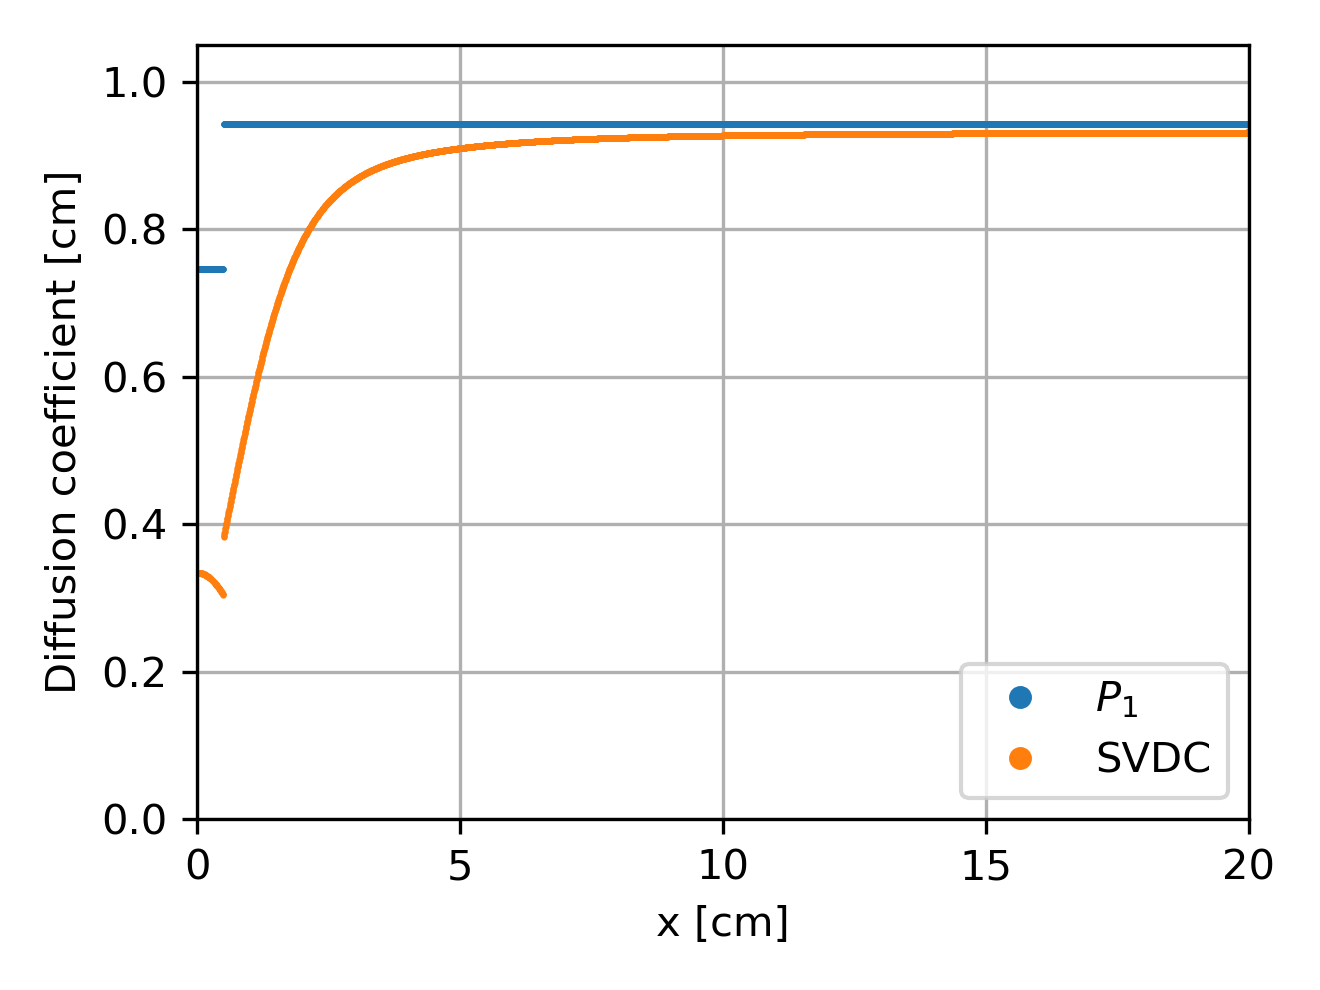
\includegraphics[width=\textwidth]{case-0-group-1-diffcoef}
    \caption{Group 1}
    \label{fig:c0g1diffcoef}
  \end{subfigure}
  \hfill
  \begin{subfigure}[b]{.49\textwidth}
    \centering
    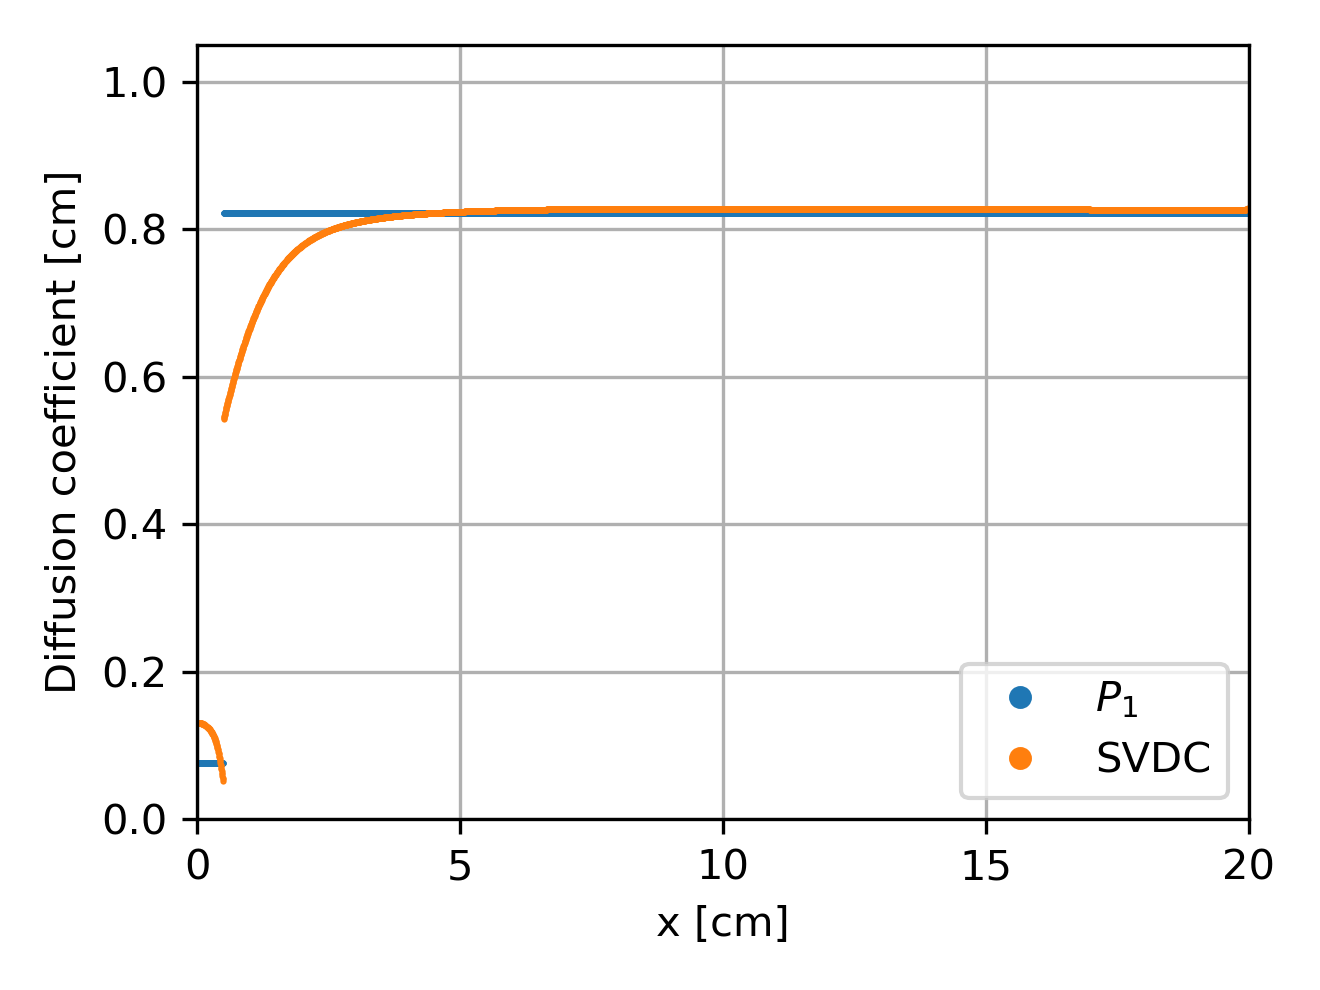
\includegraphics[width=\textwidth]{case-0-group-2-diffcoef}
    \caption{Group 2}
    \label{fig:c0g2diffcoef}
  \end{subfigure}
  \caption{$P_1$-based diffusion coefficient and \gls{SVDC} spatial distributions
  for Case 0.}
  \label{fig:c0diffcoef}
\end{figure}

Figure \ref{fig:c0flux} shows the group 1 and 2 neutron fluxes from the diffusion-$P_1$, $S_8$, and
diffusion-\gls{SVDC} solvers with a uniform mesh size of 0.005 cm. I omitted the OpenMC flux
solution because this exercise aims to demonstrate the effectiveness of \glspl{SVDC}
in reproducing an $S_N$-derived flux solution. As expected, the diffusion-$P_1$ flux solution
deviates from the $S_8$ flux solution, while the diffusion-\gls{SVDC} flux solution shows
significantly better agreement with the $S_8$ flux solution. As shown in Table \ref{table:c0k}, the
$k$ estimate from the diffusion-\gls{SVDC} solver is also closer to the $k$ estimate from the
$S_8$ solver than the diffusion-$P_1$ solver.

\begin{table}[tb!]
  \centering
  \caption{Multiplication factor $k$ estimates from the diffusion-$P_1$, $S_8$, and
  diffusion-\gls{SVDC} solvers and the absolute difference relative to the $S_8$ estimate.}
  \begin{tabular}{l S S}
    \toprule
    Solver type & {$k$} & {$k-k_{S8}$} \\
    \midrule
    $S_8$ & 0.62736 & {-} \\
    Diffusion-$P_1$ & 0.60890 & -0.01846 \\
    Diffusion-\gls{SVDC} & 0.62750 & +0.00013 \\
    \bottomrule
  \end{tabular}
  \label{table:c0k}
\end{table}

The $P_1$-based diffusion coefficients and \glspl{SVDC} in Figure \ref{fig:c0diffcoef} show good
agreement in the bulk fuel salt region far from the control rod region.
This observation supports the validity of the neutron diffusion method under the conditions
listed at the start of Section \ref{sec:svdc}. Closer to the control rod
region, the \glspl{SVDC} deviate from the $P_1$-based diffusion coefficients because the
prerequisites for diffusion theory are violated.

Another key finding from this study is that the neutron diffusion method with $P_1$-based
diffusion coefficients fails to reproduce the steep $S_8$ flux gradient in the control rod region
for group 1 and in the homogeneous fuel-graphite region adjacent to the control rod region for both
neutron groups. From a purely mathematical perspective, the streaming term in the neutron
diffusion equation requires the lower
\gls{SVDC} values in the absorber-adjacent region to induce steeper flux gradients and match the
$S_8$ flux solution. Given that highly neutron-absorbing materials induce steep flux gradients
around them, we can expect similar trends of \glspl{SVDC} being suppressed relative to
$P_1$-based diffusion coefficients in other systems with control rods. The \gls{SVDC} values within
the highly-absorbing region exhibit significant spatial variation but do not necessarily fall
below the $P_1$-based diffusion coefficients.

Thus far, this method is redundant because it requires a priori knowledge of a reference
analytical flux solution or a highly accurate numerical solution calculated using neutron
transport methods. While existing workflows for diffusion-based methods already require
computationally intensive neutron transport simulations for group constant generation, this
preprocessing step incurs a fixed computational cost through
a fixed number of neutron transport simulations. Compared to \glspl{SVDC}, $P_1$-based diffusion
coefficients behave much more like intrinsic material properties as their definitions are largely
tied to material cross sections. Variations in $P_1$-based diffusion coefficients primarily arise
from changes in the neutron energy spectrum with no direct contribution from proximity to material
interfaces (geometrical heterogeneity). $P_1$-based diffusion coefficients may be generated at
various reactor temperatures and interpolated to model the temperature dependence.

On the other
hand, the nature of \glspl{SVDC} as empirical, pointwise corrections for the diffusion equation
makes it highly dependent on the neutron flux gradient and susceptible to more significant
variations than region-wide estimates for $P_1$-based diffusion coefficients. \glspl{SVDC} will
likely need to be dynamically generated at every timestep, such as with a two-level iterative
scheme consisting of a high-level $S_N$ neutron transport calculation and a low-level neutron
diffusion calculation. In this case, the required number of neutron transport simulations scales
with the number of reactor simulations. Therefore, \gls{SVDC} generation cannot be adopted as a
one-off preprocessing step.

Another significant challenge of \glspl{SVDC} and the high-order empirical diffusion coefficients
involves their resolution near neutron flux peaks. The neutron current and flux gradient values in
Eq. \ref{eq:svdc} generally do not reach zero at the same points in space,
resulting in diffusion coefficient values tending to positive or negative infinity when the
flux gradient is close to zero. Pounders \& Rahnema avoided this issue by using
larger mesh sizes to calculate their empirical diffusion coefficients. However, their
remedy contradicts mesh convergence requirements and would worsen flux accuracy in regions with
steep, non-linear fluxes, such as near control rods. I plan to investigate and find an alternative
solution for this issue in implementing \glspl{SVDC} in the proposed work.

\subsection{Hybrid $S_N$-Diffusion Method} \label{sec:hybrid-method}

In order to reduce the computational cost of the high-level $S_N$ calculation, I propose reducing
the problem domain of the $S_N$ method to a \textit{correction region} containing the control rod
and its vicinity. Consequently, the Hybrid $S_N$-Diffusion method can retain accurate neutron flux
and current estimates around the control rod region from the $S_N$ method while making significant
computational cost savings by treating most of the reactor geometry with the neutron diffusion
method alone. Henceforth, I will refer to the $S_N$ calculation on the correction
region as the $S_N$ \textit{subproblem} or \textit{subsolver}. I define the entire problem
domain and the correction region as $\Omega^d_0$ and $\Omega^d_1$, respectively, where
$\Omega^d_1\subseteq\Omega^d_0$. The algorithm for the Hybrid $S_N$-Diffusion method is as follows:
%
\begin{enumerate}
  \item Start with an initial neutron diffusion calculation in $\Omega^d_0$ with conventional
    $P_1$-based diffusion coefficients and other standard group constants (e.g., neutron cross
    sections).
  \item Use the neutron diffusion flux estimates in $\Omega^d_1$ and current estimates along
    $\partial \Omega^d_1$ as initial and boundary conditions for the $S_N$ subsolver.
  \item With the $S_N$ subsolver, calculate an improved neutron flux solution in $\Omega^d_1$,
    which contains the control rod region and its immediate vicinity.
  \item Calculate \glspl{SVDC} using the $S_N$ flux solution and Eq. \ref{eq:svdc}.
  \item Pass the \glspl{SVDC} to the neutron diffusion solver to replace the conventional
    $P_1$ diffusion coefficients within the $\Omega^d_1$ while continuing to use $P_1$-based
    diffusion coefficients in the rest of $\Omega^d_0$.
  \item Start the next iteration by running neutron diffusion calculation with the \glspl{SVDC}
    replacing $P_1$ diffusion coefficients in part or all of $\Omega^d_1$.
  \item Repeat Steps 2-6 until convergence is reached by meeting pre-defined convergence tolerance
    values.
\end{enumerate}

\subsubsection{$S_N$ Subsolver Boundary Conditions \& Buffer Zone}

The main challenge lies in determining appropriate boundary conditions for the $S_N$ subproblem.
Given that we want to limit the coverage of $\Omega^d_1$ to the control rod region and its
immediate vicinity, $\Omega^d_1$ should be small, and the boundaries $\partial\Omega^d_1$ should
lie well within $\Omega^d_0$. Crucially, there is currently no feasible method of generating
accurate boundary fluxes for an $S_N$ solver from a neutron diffusion flux solution. In 1-D, the
standard one-group $S_N$ method requires N/2
incoming boundary flux parameters per boundary mesh point for the N/2 neutron angular fluxes
flowing into $\Omega^d_1$. The neutron diffusion method can produce at most one independent
incoming flux parameter per mesh point; this parameter is the neutron forward/backward current in
the $P_1$ approximation defined as:
%
\begin{align}
  J_{g,\pm} &= \frac{\phi_g}{4} \mp \frac{D_g}{2}\frac{d\phi_g}{dx} \label{eq:p1-j}
  \shortintertext{where}
  J_{g,\pm} &= \mbox{ neutron forward/backward current of group }g. \nonumber \\
\end{align}
%
Without additional information, the next best estimate is a uniformly
isotropic transmission of angular flux, i.e., all N/2 incoming angular fluxes $\Psi$ are equal in
magnitude. This concept is similar to the white boundary condition, which describes the uniformly
isotropic reflection of particles at a boundary, except this case involves transmission rather than
reflection. Isotropic flux transmission at $x$ can be expressed mathematically for forward angular
fluxes as:
%
\begin{align}
  \sum^N_{n=N/2+1}w_n\mu_n\Psi(x,\mu_n) =& J_{+}(x) && (\mu_n>0) \nonumber \\
  \Psi(x,\mu_n)\sum^N_{n=N/2+1}w_n\mu_n =& J_{+}(x) && (\because \mbox{isotropic transmission})
  \nonumber \\
  \Psi(x,\mu_n) =& J_{+}(x)\Bigg/\sum^N_{n=N/2+1}w_n\mu_n
\end{align}
%
and backward angular fluxes as:
%
\begin{align}
  \sum^{N/2}_{n=1}w_n\mu_n\Psi(x,\mu_n) =& J_{-}(x) && (\mu_n<0) \nonumber \\
  \Psi(x,\mu_n)\sum^{N/2}_{n=1}w_n\mu_n =& J_{-}(x) && (\because \mbox{isotropic transmission})
  \nonumber \\
  \Psi(x,\mu_n) =& J_{-}(x)\Bigg/\sum^{N/2}_{n=1}w_n\mu_n \label{eq:sn-psi-j}
\end{align}
%
These boundary conditions for the $S_N$ subsolver will generally yield inaccurate flux
$\phi$ distributions since realistic reactor systems invariably do not exhibit perfectly isotropic
neutron fluxes. However, the influence of boundary conditions on $J$ and $\frac{d\phi}{dx}$ does
not extend far from the boundaries in optically thick media. By taking the ratio of $J$
to $\frac{d\phi}{dx}$ to calculate \glspl{SVDC}, I eliminate any errors from $\phi$ since both
$J$ and $\frac{d\phi}{dx}$ scale approximately linearly with $\phi$. The \glspl{SVDC}
generated with the $S_N$ subsolver within $\Omega^d_1$ will be accurate everywhere except near
$\partial\Omega^d_1$. $\Omega^d_1$ must be large enough to provide transport corrections
through the \glspl{SVDC} and accommodate inaccurate \glspl{SVDC} near
$\partial\Omega^d_1$. The inaccurate \glspl{SVDC} should then be discarded in favor of using
$P_1$-based diffusion coefficients as in the rest of $\Omega^d_0$ not covered by $\Omega^d_0$. The
subsequent neutron diffusion calculation with this mix of \glspl{SVDC} and $P_1$-based diffusion
coefficients should provide more accurate $\phi$ and $k$ estimates than a conventional
neutron diffusion calculation.

%To resolve this issue, I posit the following hypothesis: \textit{If there exists a highly
%neutron-absorbing control rod region within the $S_N$ subproblem domain $\Omega^d_1$ and the $S_N$
%subproblem boundary $\partial\Omega^d_1$ lies several neutron mean free paths away from this
%region, the \gls{SVDC} values calculated near the control rod region (using the $S_N$ subsolver
%with isotropic hemisphere boundary conditions) will tend to the actual flux gradient solution
%(using a reference $S_N$ calculation across the entire problem domain $\Omega^d$).} In other words,
%suboptimal boundary conditions may induce inaccurate \gls{SVDC} values near the $\partial
%\Omega^d_1$ subdomain boundaries, but the \gls{SVDC} values further from $\partial\Omega^d_1$ are
%accurate and very weakly dependent on the boundary conditions. These inaccurate \gls{SVDC} values
%close to $\Omega^d_1$ may be discarded in favor of the default $P_1$-based diffusion coefficients.
%I will refer to the region containing these discarded values as the \textit{dead zone} or
%$\Omega^d_2$, where $\Omega^d_2 \subset \Omega^d_1 \subseteq \Omega^d_0$.

\subsubsection{Hybrid Method Verification with Case 0}

In this subsection, I revisit Case 0
(Figure \ref{fig:case-0-geom}) to test my hypothesis and demonstrate the Hybrid $S_N$-Diffusion
method. Once more, I defer general numerical implementation details to
Section \ref{sec:implementation}.

In Section \ref{sec:svdc}, the \gls{SVDC} generated from the reference $S_8$ calculation exhibited
significant spatial variations attributed to the presence of the control rod, as shown in Fig
\ref{fig:c0diffcoef}. The group 1 and 2 \gls{SVDC} values approach asymptotic values near the
corresponding group 1 and 2 $P_1$-based diffusion coefficient values near $x=15$ cm and $x=5$ cm,
respectively. Therefore, the $\Omega^d_1$ should, at minimum, cover the domain between $x=0$ cm and
$x=15$ cm. Allowing for a buffer region for inaccurate \glspl{SVDC} near $\partial\Omega^d_1$, I
defined $\Omega^d_1$ to span from $x=0$ cm to $x=17.5$ cm.

I set up the hybrid method to automatically determine the cutoff point, beyond which \glspl{SVDC}
in $\Omega^d_1$ are discarded, based on the \gls{SVDC} distribution generated in every iteration.
Starting from the interface between the control rod and fuel-graphite region, the algorithm sweeps
rightward for the point at which the group-wise \gls{SVDC} distribution approaches within 1\% of
the $P_1$-based diffusion coefficient value. This point serves as the cutoff point. The hybrid
method converges rapidly within two outer iterations comprising three neutron diffusion and two
$S_8$ calculations in total as outlined by the hybrid method algorithm; the change in $k$ between
the second and third outer iterations is approximately $10^{-7}$.
%
\begin{figure}[htb!]
  \centering
  \begin{subfigure}[b]{.49\textwidth}
    \centering
    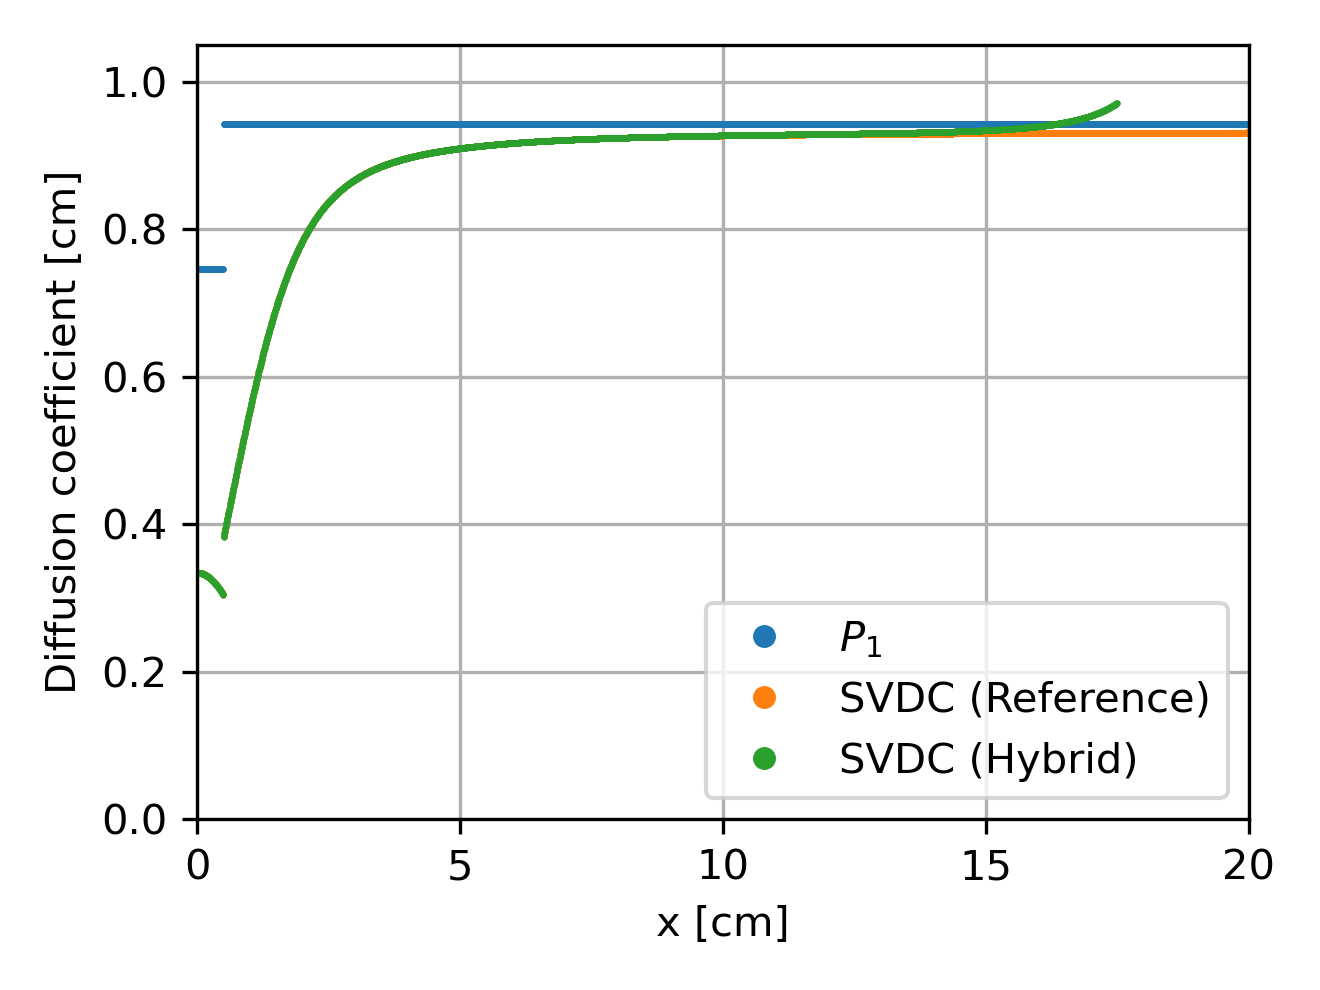
\includegraphics[width=\textwidth]{case-0-group-1-hybrid-diffcoef}
    \caption{Group 1}
    \label{fig:c0g1hd}
  \end{subfigure}
  \hfill
  \begin{subfigure}[b]{.49\textwidth}
    \centering
    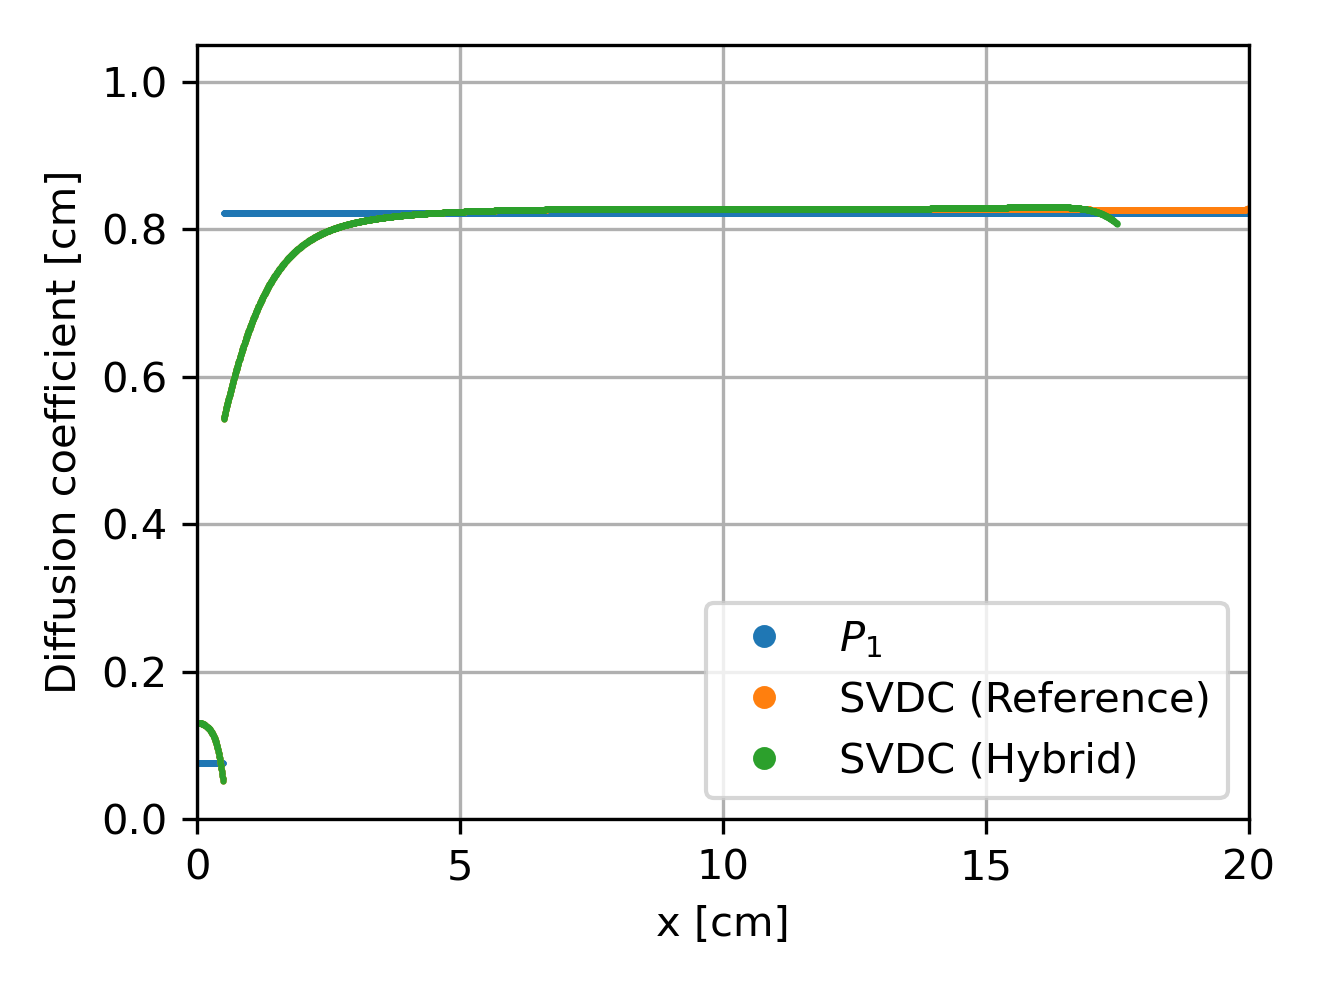
\includegraphics[width=\textwidth]{case-0-group-2-hybrid-diffcoef}
    \caption{Group 2}
    \label{fig:c0g2hd}
  \end{subfigure}
  \caption{$P_1$-based flux-limited diffusion coefficient and \gls{SVDC} spatial distribution for
  Case 0. The \gls{SVDC} distributions were generated from the reference $S_8$ (``SVDC'') and the
  hybrid (``Hybrid'') calculations.}
  \label{fig:c0hd}
\end{figure}

Refer to Figures \ref{fig:c0g1hd} and \ref{fig:c0g2hd} for a qualitative comparison of group 1 and
2 $P_1$-based diffusion coefficients, \glspl{SVDC} derived from the reference $S_8$ calculation as
demonstrated in Section \ref{sec:svdc}, and \glspl{SVDC} derived from the Hybrid $S_N$-Diffusion
method discussed here. The \glspl{SVDC} from the hybrid method agree well with the reference
\glspl{SVDC} in the control rod region and for most of the fuel-graphite region up to around
$x=15$ cm. Both sets of \glspl{SVDC} approximately coincide with the $P_1$ diffusion coefficient
values within 1\% difference from $x=14.615$ cm and $x=3.390$ cm onwards for group 1 and
group 2, respectively. Accordingly, the buffer region spans from $x=14.615$ cm to $x=17.500$ cm for
group 1 and $x=3.390$ cm to $x=17.500$ cm for group 2, in which the hybrid method defaults to the
$P_1$-based diffusion coefficients. Given that the reference \gls{SVDC} values will generally not
be known in real-world problems, the hybrid method relies on finding the intersection point of the
\gls{SVDC} and $P_1$ diffusion coefficient values to determine the buffer region cutoff point. The
size of $\Omega^d_1$ will also have to be based on where this intersection point lies.
Another important consideration is the fact that the neutron flux gradient will be discontinuous if
the \gls{SVDC} and $P_1$ diffusion coefficient values are too far apart in magnitude at the buffer
region cutoff point. A flux gradient discontinuity in a homogeneous bulk region is non-physical and
unacceptable. In Section \ref{sec:prelim-results}, I study \gls{SVDC} distribution trends
in more heterogeneous systems and their implications on determining the size of $\Omega^d_1$ and
the cutoff point.
%
\begin{figure}[htb!]
  \centering
  \begin{subfigure}[b]{.49\textwidth}
    \centering
    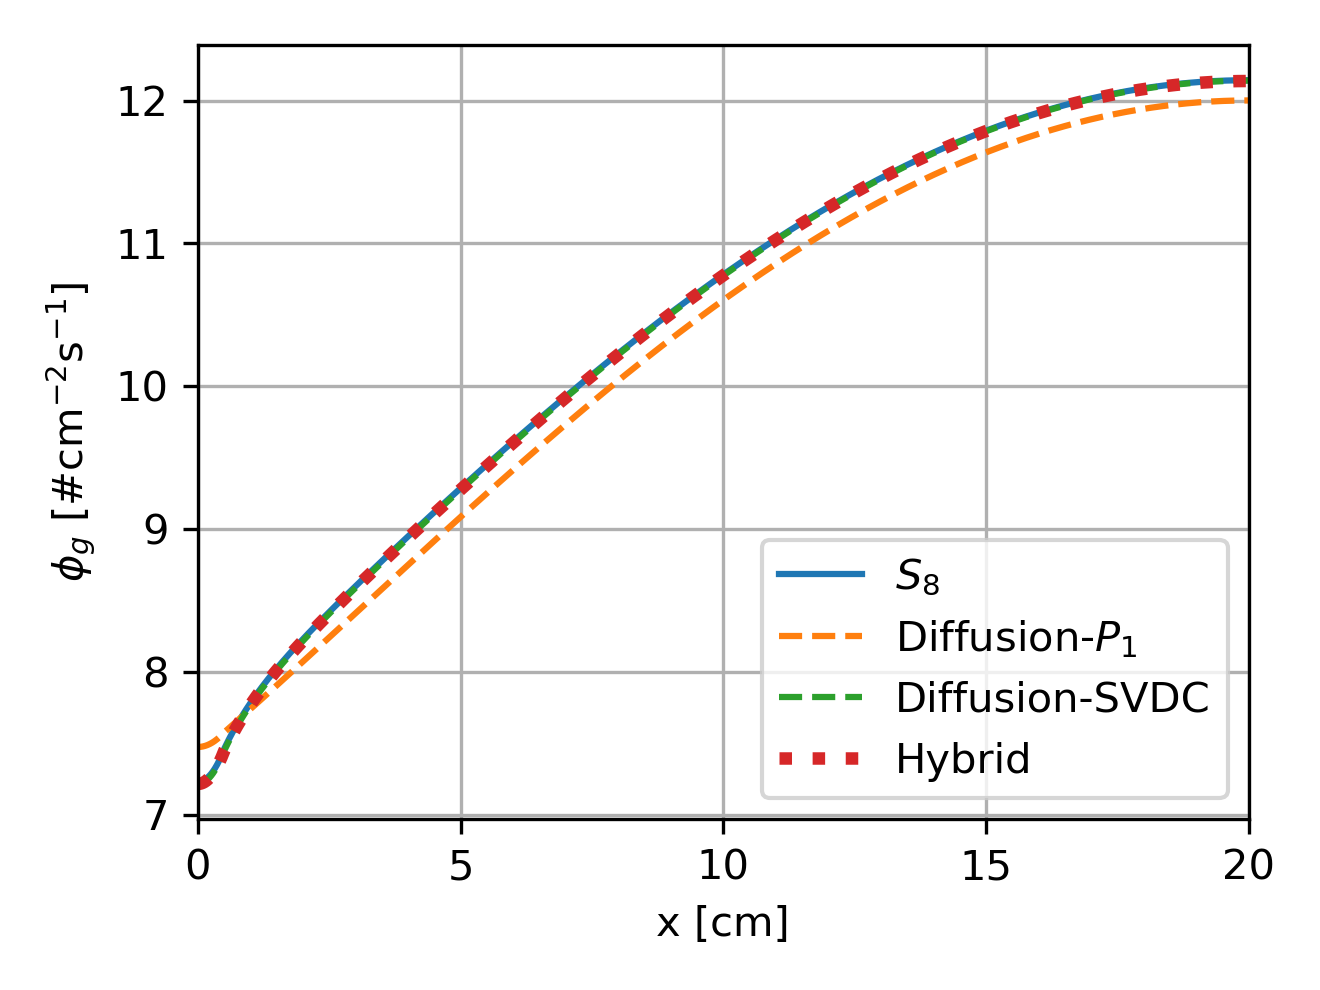
\includegraphics[width=\textwidth]{case-0-group-1-hybrid-flux}
    \caption{Group 1}
    \label{fig:c0g1hf}
  \end{subfigure}
  \hfill
  \begin{subfigure}[b]{.49\textwidth}
    \centering
    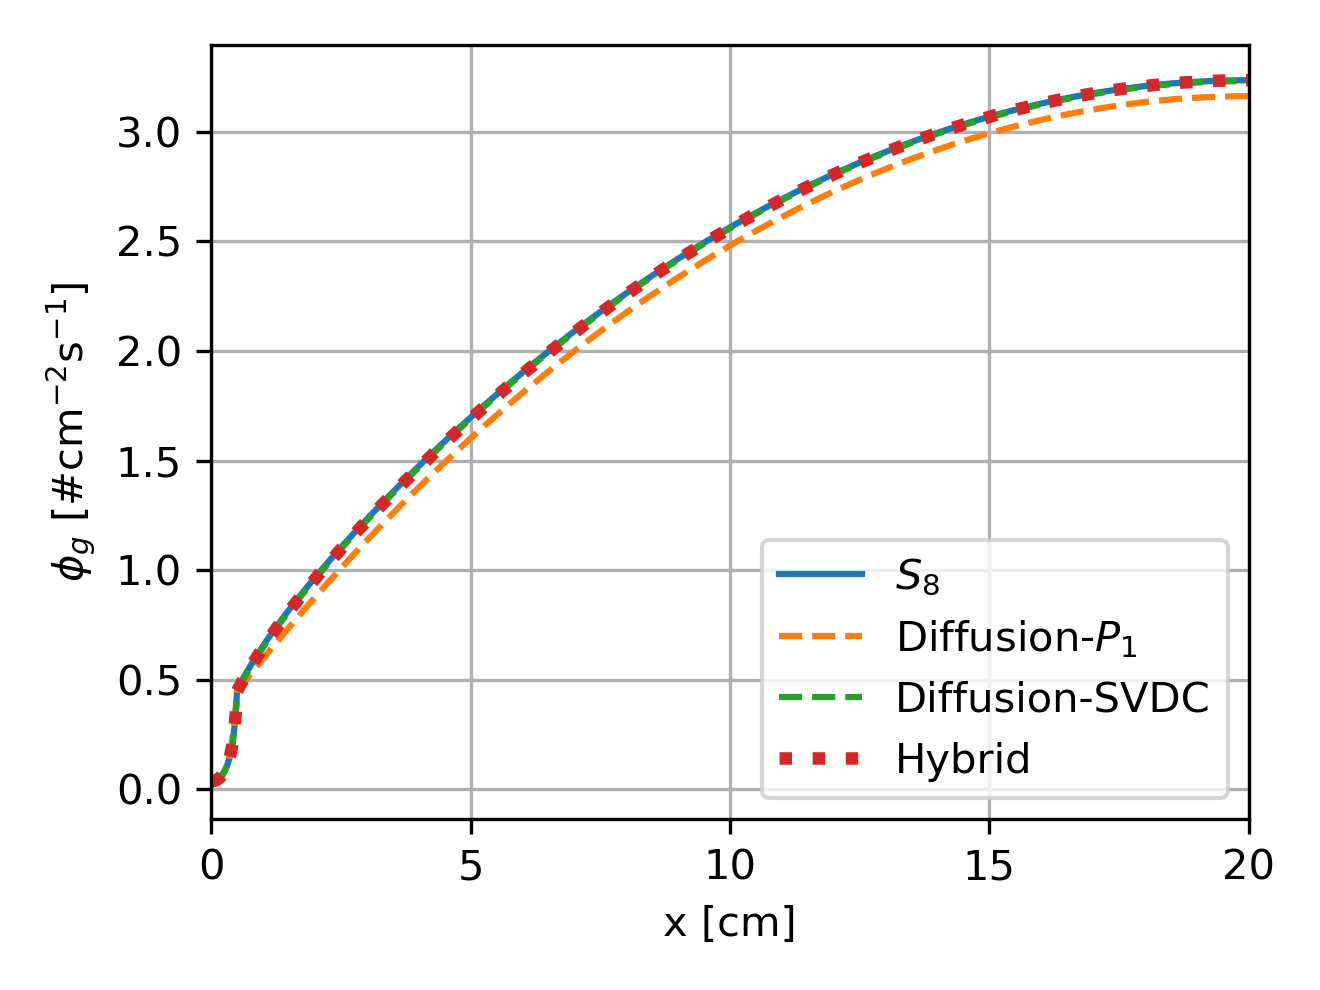
\includegraphics[width=\textwidth]{case-0-group-2-hybrid-flux}
    \caption{Group 2}
    \label{fig:c0g2hf}
  \end{subfigure}
  \caption{Neutron group 1 and 2 flux distributions from the diffusion, $S_8$, reference
  \gls{SVDC}, and hybrid methods for Case 0.}
  \label{fig:c0hf}
  \centering
  \begin{subfigure}[b]{.49\textwidth}
    \centering
    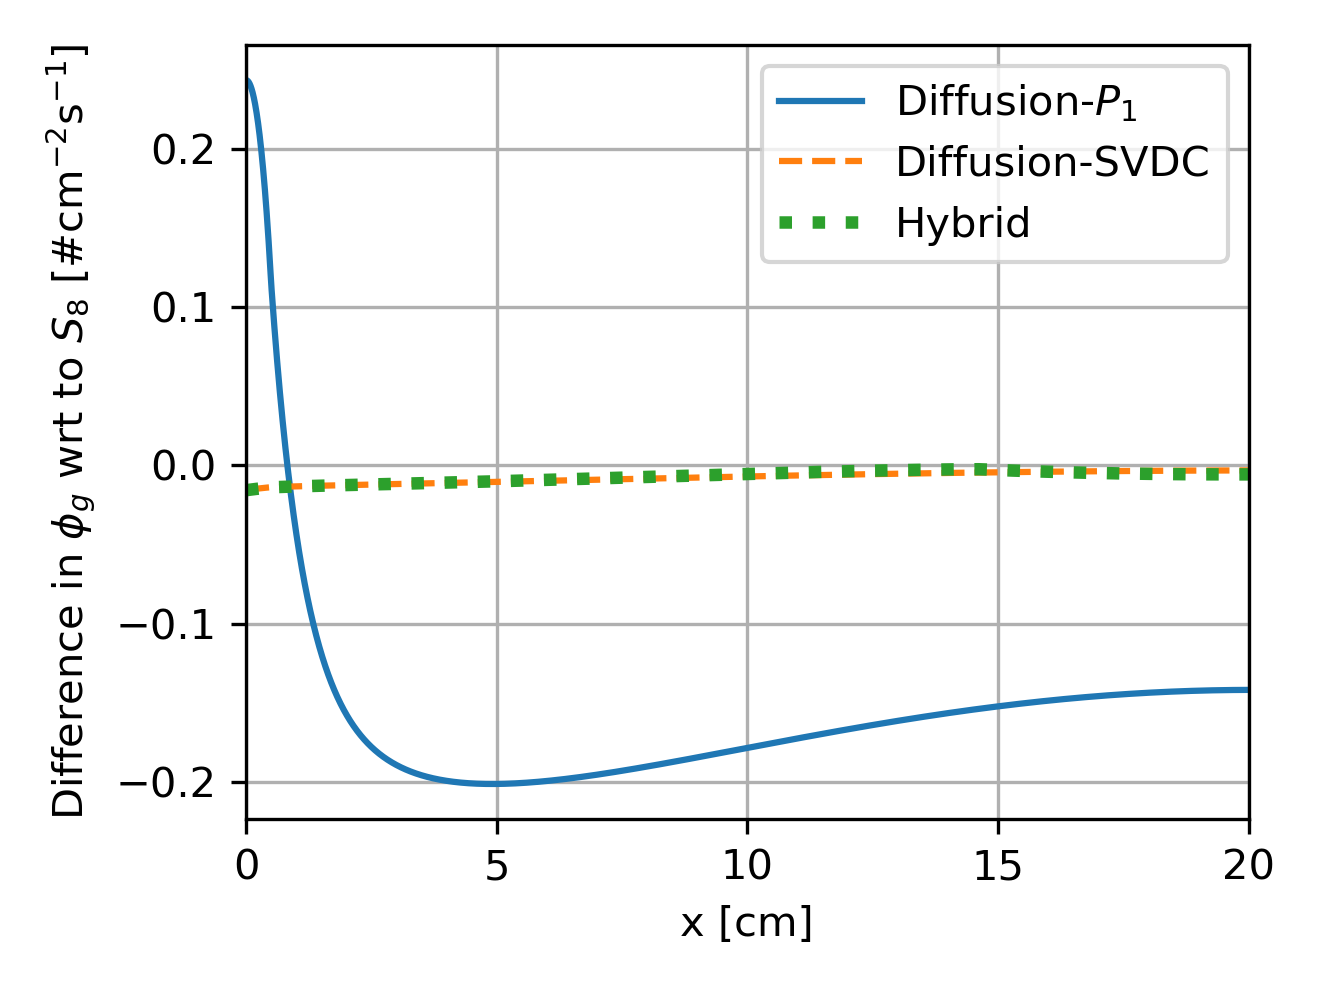
\includegraphics[width=\textwidth]{case-0-group-1-hybrid-flux-diff}
    \caption{Group 1}
    \label{fig:c0g1hfdiff}
  \end{subfigure}
  \hfill
  \begin{subfigure}[b]{.49\textwidth}
    \centering
    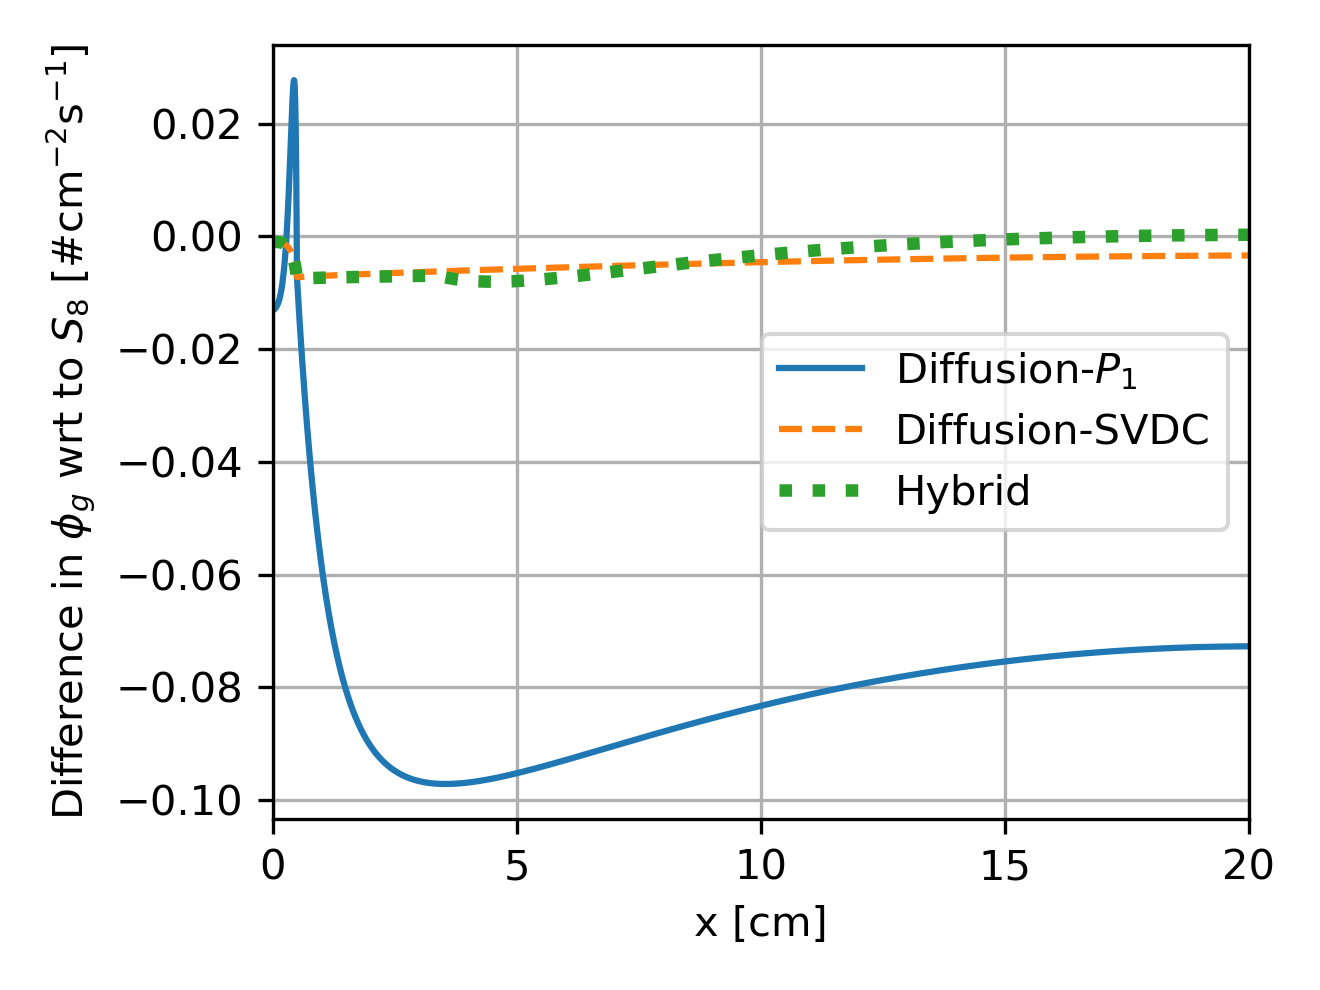
\includegraphics[width=\textwidth]{case-0-group-2-hybrid-flux-diff}
    \caption{Group 2}
    \label{fig:c0g2hfdiff}
  \end{subfigure}
  \caption{Difference in neutron group 1 and 2 flux distributions from the diffusion,
  diffusion-\gls{SVDC}, and hybrid methods with respect to the $S_8$ flux distribution for Case 0.}
  \label{fig:c0hfdiff}
\end{figure}

Figures \ref{fig:c0g1hf} and \ref{fig:c0g2hf} show the group 1 and 2 neutron flux distributions
from the various methods, while Figures \ref{fig:c0g1hfdiff} and \ref{fig:c0g2hfdiff} show the
difference in flux with respect to the $S_8$ flux distribution. As
expected following the diffusion coefficient discussion, the hybrid method flux distribution
matches the $S_8$ and Diffusion-\gls{SVDC} flux distributions well. The $k$ estimate from the
hybrid method is 0.62774, which is only 0.00024 higher than the Diffusion-\gls{SVDC} method, and
0.00038 higher than the $S_8$ method.

In Case 0, $\Omega^d_1$ covers more than half of $\Omega^d_0$ due to the control rod region being
the only significant source of influence on the neutron flux distribution in the
otherwise homogeneous system with reflective boundary conditions. I chose Case 0 as a simple test
case to aid in introducing the Hybrid $S_N$-Diffusion method. In Section \ref{sec:prelim-results},
I present more results with the hybrid method on more complicated geometries containing neutron
reflector, air, and heterogeneous fuel-graphite lattice regions and vacuum boundary conditions. In
these other test cases, the hybrid method yields smaller $\Omega^d_1$-to-$\Omega^d_0$ ratios,
reducing computational costs from running $S_N$ calculations over a relatively smaller
region.

\section{Numerical Implementation} \label{sec:implementation}

Before going into the results, this section presents numerical implementation details of group
constant data processing and the neutron diffusion, $S_N$ neutron transport, and Hybrid
$S_N$-Diffusion solvers. I implemented all numerical solvers and analysis scripts in the Python
programming language. First, I will discuss the material group constant data generation and
postprocessing steps. Next, I present the implementation details of the neutron
diffusion and $S_N$ numerical methods. Lastly, I present how they are coupled to form the Hybrid
$S_N$-Diffusion method.

\subsection{Group Constant Data Generation}

The group constants required by either or both neutron diffusion and $S_N$ neutron transport
methods are
%
\begin{itemize}
  \item $\Sigma_{t,g}$: Macroscopic total cross section in group $g$
  \item $\Sigma_{r,g}$: Macroscopic removal cross section in group $g$
  \item $\Sigma_s^{g'\rightarrow g}$: Macroscopic group-to-group scattering cross section matrix
  \item $\Sigma_{s,l}^{g'\rightarrow g}$: $l$-th Legendre moment of the macroscopic
    group-to-group scattering cross section matrix
  \item $\Sigma_{sp,l}^{g'\rightarrow g}$: $l$-th Legendre moment of the macroscopic
    group-to-group scattering production cross section matrix
  \item $D_g$: $P_1$-based diffusion coefficient in group $g$
  \item $\nu\Sigma_{f,g}$: Product of the average number of neutrons produced per fission and the
    macroscopic fission cross section in group $g$
  \item $\chi_g$: Neutron fission spectrum in group $g$
\end{itemize}
%
These group constants are generated using OpenMC's multigroup cross section generation capability
\cite{boyd_multigroup_2019} and postprocessed using a Python script into JSON format files.
$\Sigma_{r,g}$ is the only quantity that OpenMC does not directly provide. It is calculated as
%
\begin{align}
  \Sigma_{r,g} =& \sum^G_{g'\neq g}\Sigma_s^{g\rightarrow g'}+\Sigma_{a,g}-\left(\Sigma_{sp}^{g
    \rightarrow g} - \Sigma_s^{g\rightarrow g}\right)
  \shortintertext{where}
      \Sigma_{a,g} =& \mbox{ macroscopic absorption cross section in group $g$,} \nonumber \\
      \Sigma_{sp}^{g\rightarrow g} =& \mbox{ macroscopic scattering production cross section from
      group $g$ to $g$.} \nonumber
\end{align}
%
$\Sigma_{r,g}$ primarily represents the loss of neutrons from group $g$ through outscattering and
absorption. $\Sigma_{sp}^{g\rightarrow g}$ incorporates neutron multiplication effects from neutron
knockout reactions into the scattering cross section. Neutron knockout reactions are commonly
tallied as scattering reactions, and $\Sigma_{r,g}$ is a convenient term to
incorporate neutron knockout effects into the neutron diffusion equations. I ran all test cases for
$S_N$ and hybrid method calculations with up to the 2nd Legendre moments of the scattering
cross sections ($L=2$).

OpenMC uses the $P_1$ flux-limited formulation \cite{pomraning_flux-limited_1984} for calculating
$D_g$ as follows
%
\begin{align}
  D_g =& \frac{1}{3\Sigma_{tr,g}}
  \shortintertext{where}
  \Sigma_{tr,g} =& \frac{\langle\Sigma_{t,g}\phi_g\rangle-\langle\Sigma_{s1,g}\phi_g\rangle}
  {\langle\phi_g\rangle} \nonumber \\
  \langle\Sigma_{t,g}\phi_g\rangle =& \int_{r\in V}dr \int_{4\pi}d\Omega\int^{E_{g-1}}_{E_g}dE\
  \Sigma_{t,g}(r,E)\Psi(r,E,\Omega) \nonumber \\
  \langle\Sigma_{s1,g}\phi_g\rangle =& \int_{r\in V}dr \int_{4\pi}d\Omega\int^{E_{g-1}}_{E_g}dE
  \int_{4\pi}d\Omega'\int^{\infty}_0dE'\int^1_{-1}d\mu\ \mu\Sigma_s(r,E'\rightarrow E,\Omega'\cdot
  \Omega)\phi(r,E',\Omega') \nonumber \\
  \langle \phi \rangle =& \int_{r\in V}dr\int_{4\pi}d\Omega\int^{E_{g-1}}_{E_g}dE\ \Psi(r,E,\Omega)
  .\nonumber
\end{align}

\subsection{Neutron Diffusion Method}

On a 1-D uniform spatial grid with $I+1$ mesh points, the neutron scalar flux variables
$\phi_{g,i}$ are defined on the mesh points $x_i$. Theoretically, group constants are volumetric
material properties that should be defined on the cell-centered half-integer mesh points
$x_{i+\sfrac{1}{2}}$. In practice, all material properties except diffusion coefficients are
uniform in each subregion and sampled at $x_i$. To avoid ambiguity concerning diffusion
coefficient sampling, I formulated all test cases such that all material interfaces fall on $x_i$.

Discretizing the multigroup $k$-eigenvalue neutron diffusion equations in Eq. \ref{eq:1d-diff}
and reformulating the scattering term using neutron balance in the control volume bounded by
$x_{i-\sfrac{1}{2}}$ and $x_{i+\sfrac{1}{2}}$ yields
%
\begin{align}
  J_{g,i+\sfrac{1}{2}} - J_{g,i-\sfrac{1}{2}} + \Sigma_{t,g,i} \phi_{g,i} \Delta x = \sum^G_{g'=1}\left[
  \Sigma_{s,i}^{g'\rightarrow g}\phi_{g',i} + \chi_{g,i}\frac{\nu\Sigma_{f,g',i}}{k} \phi_{g',i}
\right]\Delta x. \label{eq:diff-j}
\end{align}
%
Using the diamond difference scheme to replace the $J$ terms with the discretized form of
Fick's first law of diffusion,
%
\begin{align}
  J_{g,i+\sfrac{1}{2}} = -D_{g,i+\sfrac{1}{2}}\frac{d\phi_{g,i+\sfrac{1}{2}}}{dx} =
  -D_{g,i+\sfrac{1}{2}} \frac{\phi_{g,i+1}-\phi_{g,i}}{\Delta x},
\end{align}
%
and rearranging the terms in Eq. \ref{eq:diff-j} yields
%
\begin{align}
  -\frac{D_{g,i-\sfrac{1}{2}}}{\Delta x} \phi_{g,i-1} + &\left[\frac{D_{g,i-\sfrac{1}{2}}+
  D_{g,i+\sfrac{1}{2}}}{\Delta x} + \Delta x\ \Sigma_{r,g,i} \right]\phi_{g,i} -
  \frac{D_{g,i+\sfrac{1}{2}}}{\Delta x}\phi_{g,i+1} -\Delta x\sum^G_{g'\neq g}
  \Sigma_{s,i}^{g'\rightarrow g}\phi_{g',i} \nonumber \\
  =& \Delta x\sum^G_{g'=1}
  \chi_{g,i} \frac{\nu\Sigma_{f,g',i}}{k} \phi_{g',i}, \label{eq:diff-fd}
  \shortintertext{where}
  \Sigma_{r,g} =& \Sigma_{t,g} - \Sigma_s^{g\rightarrow g} \nonumber \\
  =& \mbox{ macroscopic removal cross section for neutron group }g. \nonumber
\end{align}
%
The diamond difference scheme is 2nd-order accurate, and this form is
equivalent to applying 2nd-order finite differencing to the original neutron diffusion equation in
Eq. \ref{eq:1d-diff} with diamond differencing for the cell-centered group constants.
The fixed neutron source $S_g$ is ignored here since the test cases are all neutron-multiplying
systems with no fixed source.

I implemented two types of boundary conditions: vacuum and reflective boundary conditions. The
\textbf{vacuum boundary conditions} are imposed by setting the incoming flux in the $P_1$
approximation to zero and applying 2nd-order finite differencing as follows:
%
\begin{align}
  \mbox{Left boundary: } \frac{\phi_{g,0}}{4}-\frac{D_{g,\sfrac{1}{2}}}{2}
  \frac{\left(-\phi_{g,2}+4\phi_{g,1}-3\phi_{g,0}\right)}{2\Delta x} =& 0 \\
  \mbox{Right boundary: } \frac{\phi_{g,I}}{4}+\frac{D_{g,I-\sfrac{1}{2}}}{2}
  \frac{\left(\phi_{g,I-2}-4\phi_{g,I-1}+3\phi_{g,I}\right)}{2\Delta x} =& 0.
\end{align}
%
The \textbf{reflective boundary conditions} are imposed by setting the flux gradient to zero and
applying 2nd-order finite differencing as follows:
%
\begin{align}
  \mbox{Left boundary: } \frac{-3\phi_{g,0}+4\phi_{g,1}-\phi_{g,2}}{2\Delta x} =& 0 \\
  \mbox{Right boundary: } \frac{3\phi_{g,I}-4\phi_{g,I-1}+\phi_{g,I-2}}{2\Delta x} =& 0
\end{align}
%
At material interfaces, the continuity condition requires that the net neutron current on either
side of the interface be equal as follows:
%
\begin{align}
  -\frac{3D_{g,i-\sfrac{1}{2}} - D_{g,i-\sfrac{3}{2}} }{2}
  \frac{\phi_{g,i-2}-4\phi_{g,i-1}+3\phi_{g,i}}{2\Delta x} =&
  -\frac{3D_{g,i+\sfrac{1}{2}} - D_{g,i+\sfrac{3}{2}} }{2}
  \frac{-3\phi_{g,i}+4\phi_{g,i+1}-\phi_{g,i}}{2\Delta x} \label{eq:itf-bc}
\end{align}
%
for a material interface at $x_i$.

Altogether, they form a system of equations of the form $\bm{A\overline{\phi}}=\bm{\frac{1}{k}
B\overline{\phi}}$, where $\bm{\overline{\phi}}$ is a flattened vector representation of
$\phi_{g,i}$, and $\bm{A}$ and $\bm{B}$ are matrices of the coefficients of $\phi_{g,i}$ as given
by Eqs. \ref{eq:diff-fd} to \ref{eq:itf-bc}. I implemented the inverse power method to find $k$ and
$\overline{\phi}$. The inverse power method algorithm is as follows
%
\begin{align}
  \shortintertext{1. Initialize $k^0$ and $\bm{\overline{\phi}}^0$}
  \shortintertext{2. Update $\bm{\overline{\phi}}$ and $k$}
  \bm{\overline{\phi}}^m =& \frac{1}{k^{m-1}}\bm{A}^{-1}\bm{B\overline{\phi}}^{m-1} \\
  k^m =& k^{m-1}\frac{|\bm{B\overline{\phi}}^m|}{|\bm{B\overline{\phi}}^{m-1}|}
  \shortintertext{3. Check whether convergence is reached}
  \epsilon_\phi =
  \frac{|\bm{\overline{\phi}}^m-\bm{\overline{\phi}}^{m-1}|}{|\bm{\overline{\phi}}^m|} <& \
  tol_{\bm{\overline{\phi}}} \\
  \epsilon_k =
  \frac{|k^m-k^{m-1}|}{|k^m|} <& \ tol_k
  \shortintertext{4. Return to Step 2 if either expression is false, otherwise exit.} \nonumber
\end{align}
%
$k^m$ and $\overline{\phi}^m$ denote estimates of $k$ and $\overline{\phi}$ after the $m$-th
iteration. Matrix $\bm{A}$ is a primarily tridiagonal matrix with at most $G-1$ off-diagonal terms
from the fourth term in Eq. \ref{eq:diff-fd}. Thus, $\bm{A}$ is initialized as a sparse matrix to
take advantage of the computationally efficient sparse matrix solver functions from the
\texttt{sparse} class of the \texttt{SciPy} Python library for scientific and technical computing.
Matrix $\bm{B}$
is never initialized explicitly as a matrix. Instead, the vector $\bm{b}=\bm{B\overline{\phi}}$ is
updated directly in every iteration. In this system of equations, $|\bm{b}|$ corresponds to the
total number of fission neutrons produced in the system for a given $\bm{\overline{\phi}}$. This
quantity is calculated using the \texttt{trapezoid} numerical integration function from
\texttt{SciPy} to estimate the integral value of $\nu\Sigma_{g,f}\phi_{g}$ in $x$ from the discrete
flux values in $\bm{x}$. Finally, the final $\phi_{g,i}$ is normalized by a factor of $|\bm{b}|/k$
(no. of source neutrons) to obtain the neutron scalar flux per source neutron.

\subsection{$S_N$ Neutron Transport Method}

For the 1-D $S_N$ neutron transport method on the same uniform spatial grid with $I+1$ mesh points,
the neutron angular flux variables $\Psi_{g,i,n}=\Psi_g(x_i,\mu_n)$ are defined on the mesh points
$x_i$ while neutron scalar flux variables $\phi_{g,i\pm\sfrac{1}{2}}=\phi_g(x_{i\pm\sfrac{1}{2}})$
are defined on the half-integer mesh points $x_{i\pm\sfrac{1}{2}}$. All group constants are sampled
at $x_{i\pm\sfrac{1}{2}}$.

The $S_N$ equations are solved using the transport sweep method in which the algorithm ``sweeps''
through the spatial grid and sequentially updates $\Psi_{g,i,n}$. The algorithm sweep
direction follows the direction of neutron travel, i.e. it sweeps in the positive direction for
$\Psi_{g,i,n}$ with $\mu_n>0$ and vice versa. Doing otherwise is unphysical and causes numerical
instabilities.

Discretizing the multigroup $S_N$ neutron transport equations in Eq. \ref{eq:1d-sn} about
$x_{i+\sfrac{1}{2}}$ yields
%
\begin{align}
  \mu_n\frac{\Psi_{g,i+1,n}-\Psi_{g,i,n}}{x_{i+1}-x_i} + \Sigma_{t,g,i+\sfrac{1}{2}}
  \Psi_{g,i+\sfrac{1}{2},n} = q_{g,i+\sfrac{1}{2},n}
\end{align}
%
where $q_{g,i+\sfrac{1}{2},n}$ represents the combined scattering and fission neutron source term.
After expressing $\Psi_{g,i+\sfrac{1}{2}}$ as the average of $\Psi_{g,i+1,n}$ and $\Psi_{g,i,n}$
in the diamond difference scheme and rearranging the terms, we obtain
%
\begin{align}
  \Psi_{g,i+1,n} =& \frac{1-\Sigma_{t,g}\Delta x/2\mu_n}{1+
    \Sigma_{t,g}\Delta x/2\mu_n}\Psi_{g,i,n} +
    q\frac{\Delta x}{\mu_n\left(1+\Sigma_{t,g}\Delta x/2\mu_n\right)} \label{eq:sweep-right} &&
    (\mbox{for } \mu_n > 0)
\shortintertext{and}
  \Psi_{g,i,n} =& \frac{1+\Sigma_{t,g}\Delta x/2\mu_n}{1-
    \Sigma_{t,g}\Delta x/2\mu_n}\Psi_{g,i+1,n} -
    q\frac{\Delta x}{\mu_n\left(1-\Sigma_{t,g}\Delta x/2\mu_n\right)}. \label{eq:sweep-left} &&
    (\mbox{for } \mu_n < 0)
\end{align}
%
The remaining $i+\sfrac{1}{2}$ indexes on the group constants are dropped to reduce visual clutter.
These expressions are used to update $\Psi_{g,i,n}$ in the forward and backward transport sweeps.

The discretized scattering and fission terms in $q_{g,i+\sfrac{1}{2},n}$ are given as
%
\begin{align}
  q_{g,i+\sfrac{1}{2},n} =& \sum^G_{g'=1}\sum^L_{l=0}\frac{\left(2l+1\right)}
  {2}\Sigma_{s,l}^{g'\rightarrow g}P_l(\mu_n)\phi_{l,g',i+\sfrac{1}{2}} \nonumber \\
  &+\frac{\chi_g}{2}\sum^G_{g'=1}\frac{\nu\Sigma_{f,g'}}{k}\phi_{0,g',i+\sfrac{1}{2}}
  \label{eq:sn-q}
  \shortintertext{where}
  \phi_{l,g',i+\sfrac{1}{2}} =& \sum^N_{n'=1}w_{n'}P_l(\mu_{n'})\frac{\Psi_{g',i,n'}+
  \Psi_{g',i+1,n'}}{2}. \label{eq:phi-l}
\end{align}
%
$\phi_{l,g,i}$ are $l$-th Legendre expansions of the neutron flux evaluated using Gauss-Legendre
quadrature over $\mu_{n'}=[-1,1]$. $\phi_{0,g,i}$ and $\phi_{1,g,i}$ also correspond to the neutron
scalar flux $\phi_{g,i}$ and net current $J_{g,i}$, respectively.

For vacuum boundary conditions, $\Psi_{g,0,n}$ is zero for all positive $\mu_n$ while
$\Psi_{g,I,n}$ is zero for all negative $\mu_n$ as follows
%
\begin{align}
  \mbox{Left boundary: } \Psi_{g,0,n} =& 0 && (\mbox{for } \mu_n > 0) \\
  \mbox{Right boundary: } \Psi_{g,I,n} =& 0 && (\mbox{for } \mu_n < 0)
\end{align}
%
Reflective boundary conditions are imposed by equating the incoming angular flux to the
outgoing angular flux in the opposite direction as follows
%
\begin{align}
  \mbox{Left boundary: } \Psi_{g,0,n} =& \Psi_{g,0,n'} && (\mbox{for } \mu_n > 0, \mu_n =
  -\mu_{n'}) \\
  \mbox{Right boundary: } \Psi_{g,I,n} =& \Psi_{g,I,n'} && (\mbox{for } \mu_n < 0, \mu_n =
  -\mu_{n'})
\end{align}

The power iteration algorithm for the $S_N$ method is similar to the inverse power method algorithm
applied in the neutron diffusion method. The transport sweep step replaces the matrix-solving step
for updating $\overline{\phi}$.
%
\begin{align}
  \shortintertext{1. Initialize $k^0$, $\phi_{l,g,i+\sfrac{1}{2}}^0$, and $q^0$}
  \shortintertext{2. Apply transport sweeps to solve for $\Psi^m$ using Eqs. \ref{eq:sweep-right},
  \ref{eq:sweep-left}, and \ref{eq:sn-q}}
  \shortintertext{3. Update $\phi^m$ and $k^m$ using Eqs. \ref{eq:phi-l} and \ref{eq:sn-k}}
  k^m =& k^{m-1}\frac{\sum^I_{i=0}\sum^G_{g=1}\nu\Sigma_{f,g}\phi^m_{g,i+\sfrac{1}{2}}}
  {\sum^I_{i=0}\sum^G_{g=1}\nu\Sigma_{f,g}\phi^{m-1}_{g,i+\sfrac{1}{2}}} \label{eq:sn-k}
  \shortintertext{4. Check whether convergence is reached}
  \epsilon_\phi =
  \frac{|\bm{\overline{\phi}}^m-\bm{\overline{\phi}}^{m-1}|}{|\bm{\overline{\phi}}^m|} <& \
  tol_{\bm{\overline{\phi}}} \\
  \epsilon_k =
  \frac{|k^m-k^{m-1}|}{|k^m|} <& \ tol_k
  \shortintertext{5. Return to Step 2 if either expression is false, otherwise exit.} \nonumber
\end{align}

The transport sweep and $\phi^m$-update algorithms are parallelized using the \texttt{joblib}
parallel computing Python library \cite{noauthor_joblib_nodate} across all available CPU threads.
The total computational work is subdivided into several smaller tasks classified by unique pairs
of $g$ and $n$ values; each thread computes all $\Psi^m$ or $\phi^m$ values on the mesh for a given
pair of indexes $g$ and $n$.

\subsection{Hybrid $S_N$-Diffusion Method}

Without loss of generality, consider a 1-D system symmetric about the left boundary at $x_0=0$ cm.
Like Case 0, the control rod region is the left-most region, followed by other regions. The $S_N$
subproblem domain $\Omega^d_1$ is bounded by $x_0$ and $x_j$ for some $x_j$
located several mean free paths to the right of the control rod region as governed by the relevant
discussion in Section \ref{sec:hybrid-method}.

Excluding the initial neutron diffusion calculation to initialize $k^0$ and $\phi^0$, each outer
iteration in the hybrid method consists of one $S_N$ neutron transport calculation and one neutron
diffusion calculation. The $\phi$ estimates from these $S_N$ transport and neutron diffusion
calculations are labeled as $\phi^{m+\sfrac{1}{2}}$ and $\phi^{m+1}$ during the
$(m+1)$-th outer iteration. $\phi^{m+\sfrac{1}{2}}$ spans $\Omega^d_1$ while $\phi^{m+1}$ spans
the entire domain $\Omega^d_0$.

For the $S_N$ subproblem boundary conditions, we discretize Eqs. \ref{eq:p1-j} and
\ref{eq:sn-psi-j} as follows
%
\begin{align}
  \Psi_{g,j,n} =& \frac{J_{g,-}(x_j)}{\sum^{N/2}_{n'=1}w_{n'}\mu_{n'}} \nonumber \\
  =& \frac{\frac{\phi_g(x_j)}{4}+
  \frac{D_g(x_{j-\sfrac{1}{2}})}{2}\frac{d\phi_g(x_j)}{dx}}{\sum^{N/2}_{n'=1}w_{n'}\mu_{n'}}
  \nonumber \\
  =& \frac{\frac{\phi_{g,j}}{4}+
  \frac{D_{g,j-\sfrac{1}{2}}}{2}\frac{\phi_{g,j}-\phi_{g,j-1}}{\Delta x}}
    {\sum^{N/2}_{n'=1}w_{n'}\mu_{n'}} && (\mu_n < 0) \label{eq:sn-bc}
\end{align}
%
where $D_g$ is the $P_1$-based diffusion coefficient value.

The \gls{SVDC} formulation in Eq. \ref{eq:svdc} is discretized using the diamond difference scheme
as follows
%
\begin{align}
  D^s_{g,i+\sfrac{1}{2}} =& -\frac{J^{tr}_{g,i+1}+J^{tr}_{g,i}}{2} \left(
  \frac{\phi^{tr}_{g,i+1}-\phi^{tr}_{g,i}}{\Delta x} \right)^{-1} = -\frac{\Delta x}{2}
  \frac{J^{tr}_{g,i+1}+J^{tr}_{g,i}}{\phi^{tr}_{g,i+1}-\phi^{tr}_{g,i}}. \label{eq:svdc-num}
\end{align}
%
%From Eq. \ref{eq:svdc-num}, we note that numerical instabilities may occur near flux peaks where
%the flux gradient and thus the denominator of Eq. \ref{eq:svdc-num} approach zero. On the other
%hand, this observation also implies that diffusion coefficient values have negligible influence on
%the flux solution near flux peaks due to the small flux gradient values. Therefore, we can avoid
%numerical instabilities by applying the following logic after calculating $D^s_g$: If the ratio of
%$|\frac{d\phi_g}{dx}|$ to $|\phi_g|$ is sufficiently small and $|D^s_g-D_g| > D_g$, the hybrid
%method defaults to using $D_g$ instead of $|D^s_g-D_g|$. The first conditional statement locates
%regions of relatively flat flux, and of these regions, the second conditional statement excludes
%regions which naturally experience flat flux such as air-filled regions. In all test cases,
%applying the first conditional as $|\frac{1}{\phi_g}\frac{d\phi_g}{dx}|<5\times 10^{-2}$ was
%sufficient for this task.

The Hybrid $S_N$-Diffusion algorithm is as follows
%
\begin{align}
  \shortintertext{1. Initialize $k^0$ and $\phi^0$ with an initial neutron diffusion calculation on
  $\Omega^d_0$}
  \shortintertext{2. Generate estimates for $\Psi_{g,j,n}$ at $x_j$ for the $S_N$ transport
  calculation boundary conditions using Eq. \ref{eq:sn-bc}}
  \shortintertext{3. Calculate $\phi^{m+\sfrac{1}{2}}$ with the $S_N$ transport subsolver on
  $\Omega^d_1$}
  \shortintertext{4. Generate \glspl{SVDC} with $\phi^{m+\sfrac{1}{2}}$ and $J^{m+\sfrac{1}{2}}$
  using Eq. \ref{eq:svdc-num}}
  \shortintertext{5. Calculate $\phi^{m+1}$ with the newly generated \glspl{SVDC} and the neutron
  diffusion solver on $\Omega^d_0$}
  \shortintertext{6. Check whether convergence is reached}
  \frac{|\bm{\overline{\phi}}^m-\bm{\overline{\phi}}^{m-1}|}{|\bm{\overline{\phi}}^m|} <& \
  tol_{\bm{\overline{\phi}}} \\
  \frac{|k^m-k^{m-1}|}{|k^m|} <& \ tol_k
  \shortintertext{7. Return to Step 2 if either expression is false, otherwise exit.} \nonumber
\end{align}
%
Generally, the convergence tolerance values for the outer hybrid method iteration must be smaller
than the tolerance values for the neutron diffusion and $S_N$ transport inner iterations. Using
$\phi^m$ from the neutron diffusion calculation as initial conditions for the $S_N$ transport
calculation in the $(m+1)$-th iteration helps to reduce the number of transport
sweeps required significantly.

The $S_N$ subsolver only covers $\Omega^d_1$, so it does not calculate an independent $k$
estimate. Instead, the $k^m$ from the neutron diffusion calculation scales the fission neutron
source term in the $S_N$ subsolver.

\section{Description of 1-D Test Cases} \label{sec:test-case}

I designed ten 1-D test cases with increasing complexity to test the performance of the Hybrid
$S_N$-Diffusion method in response to various geometrical features. The latter cases resemble the
reference \gls{MSRE} design \cite{robertson_msre_1965}, which has centrally located control rods
and air-filled rod guide tubes. Figure \ref{fig:case-geom} shows the geometries of Cases 0 to
5b. All geometries have reflective boundary conditions at $x=0$ cm to reduce computational costs by
creating half-core or repeating unit cell models. Cases 1a, 2a, 3a, and 4a are repeating unit
cell models with reflecting boundaries on the right-side boundaries. Cases 1b, 2b, 3b, 4b, 5a, and
5b are half-core models with vacuum boundaries on the right-side boundaries.

Starting with an infinite, homogeneous region in Case 1a, I systematically added geometric
complexities to each successive test case to identify how each feature impacts the neutronics
results. Case 1b introduces a reflector region and vacuum boundary conditions relative to Case 1a.
Cases 2a and 2b introduce a control rod region between $x=0$ cm and $x=0.5$ cm relative to Cases 1a
and 1b. Cases 3a and 3b introduce a 0.5 cm-thick air gap between the control rod and the
fuel-graphite mixture regions relative to Cases 2a and 2b. For Cases 4a and 4b, I replaced the
homogeneous fuel-graphite mixture in Cases 1a and 2b with explicit fuel-graphite lattices, as shown
in Figure \ref{fig:case-geom}. Case 5a introduces an air gap between the control rod and the
fuel-graphite lattice regions. Lastly, Case 5b replaces the control rod region with an extended
air gap region to provide a base case for the control rod worth calculations relative to Case 5a.

\begin{figure}[htb!]
  \centering
  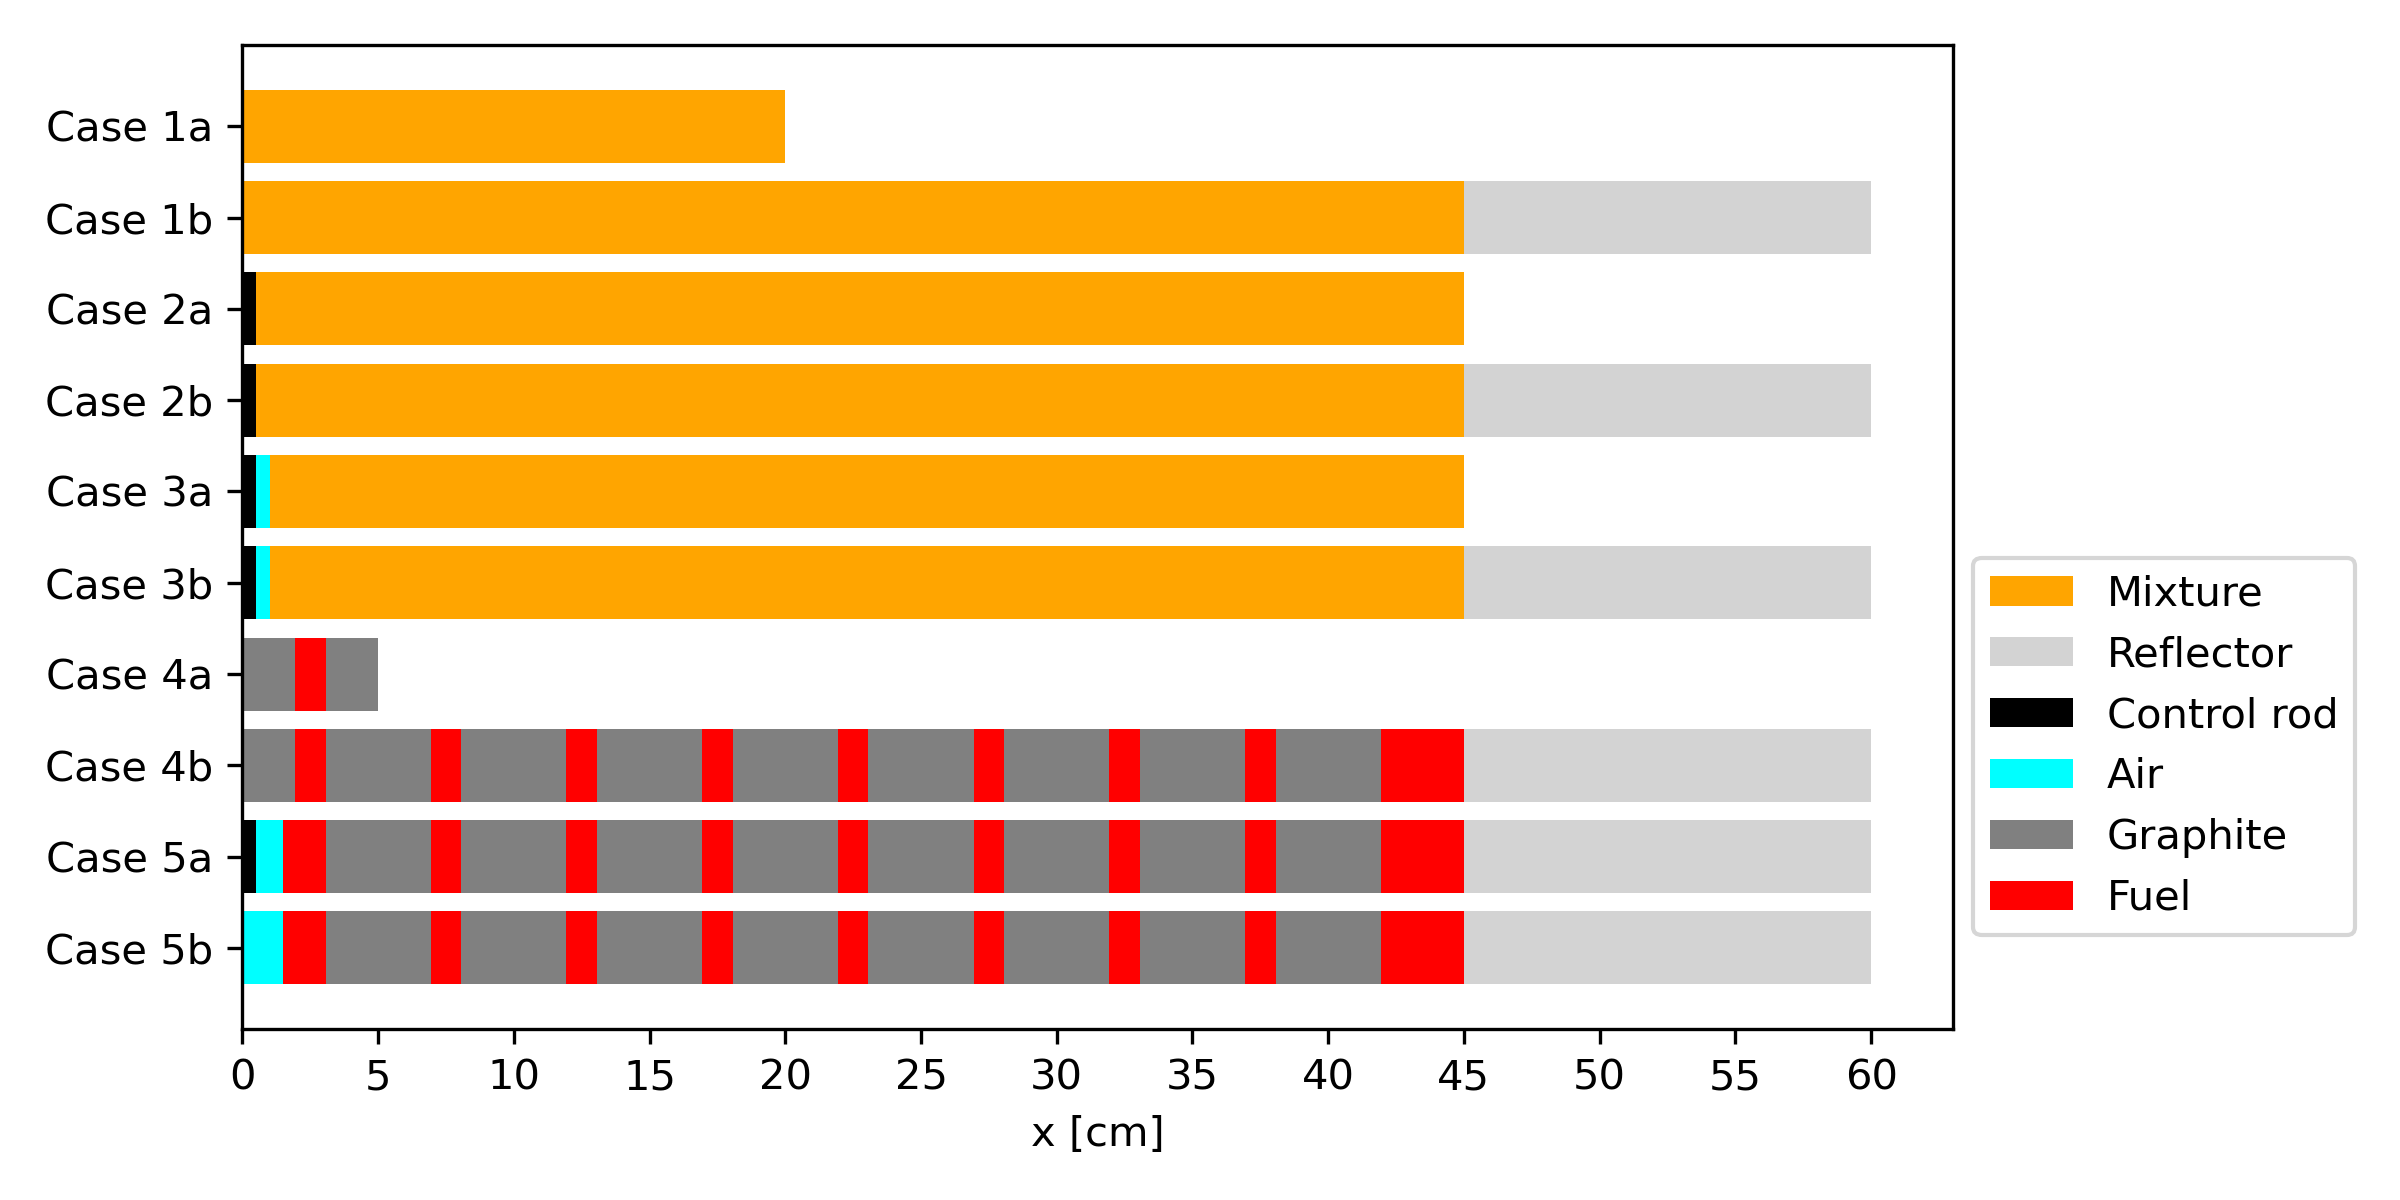
\includegraphics[width=\columnwidth]{case-geometry}
  \caption{Geometries of the 1-D test cases. The material labeled ``mixture'' represents a
    homogeneous mixture of fuel and graphite at a ratio of 22.5\%-77.5\% by volume. All geometries
    have reflective boundary conditions on the boundary at $x=0$ cm. The right-side boundaries are
    reflective for Cases 1a, 2a, 3a, and 4a, and vacuum for Cases 1b, 2b, 3b, 4b, 5a, and 5b.}
  \label{fig:case-geom}
\end{figure}
%
\begin{figure}[htb!]
  \centering
  \begin{subfigure}[t]{.49\textwidth}
    \centering
    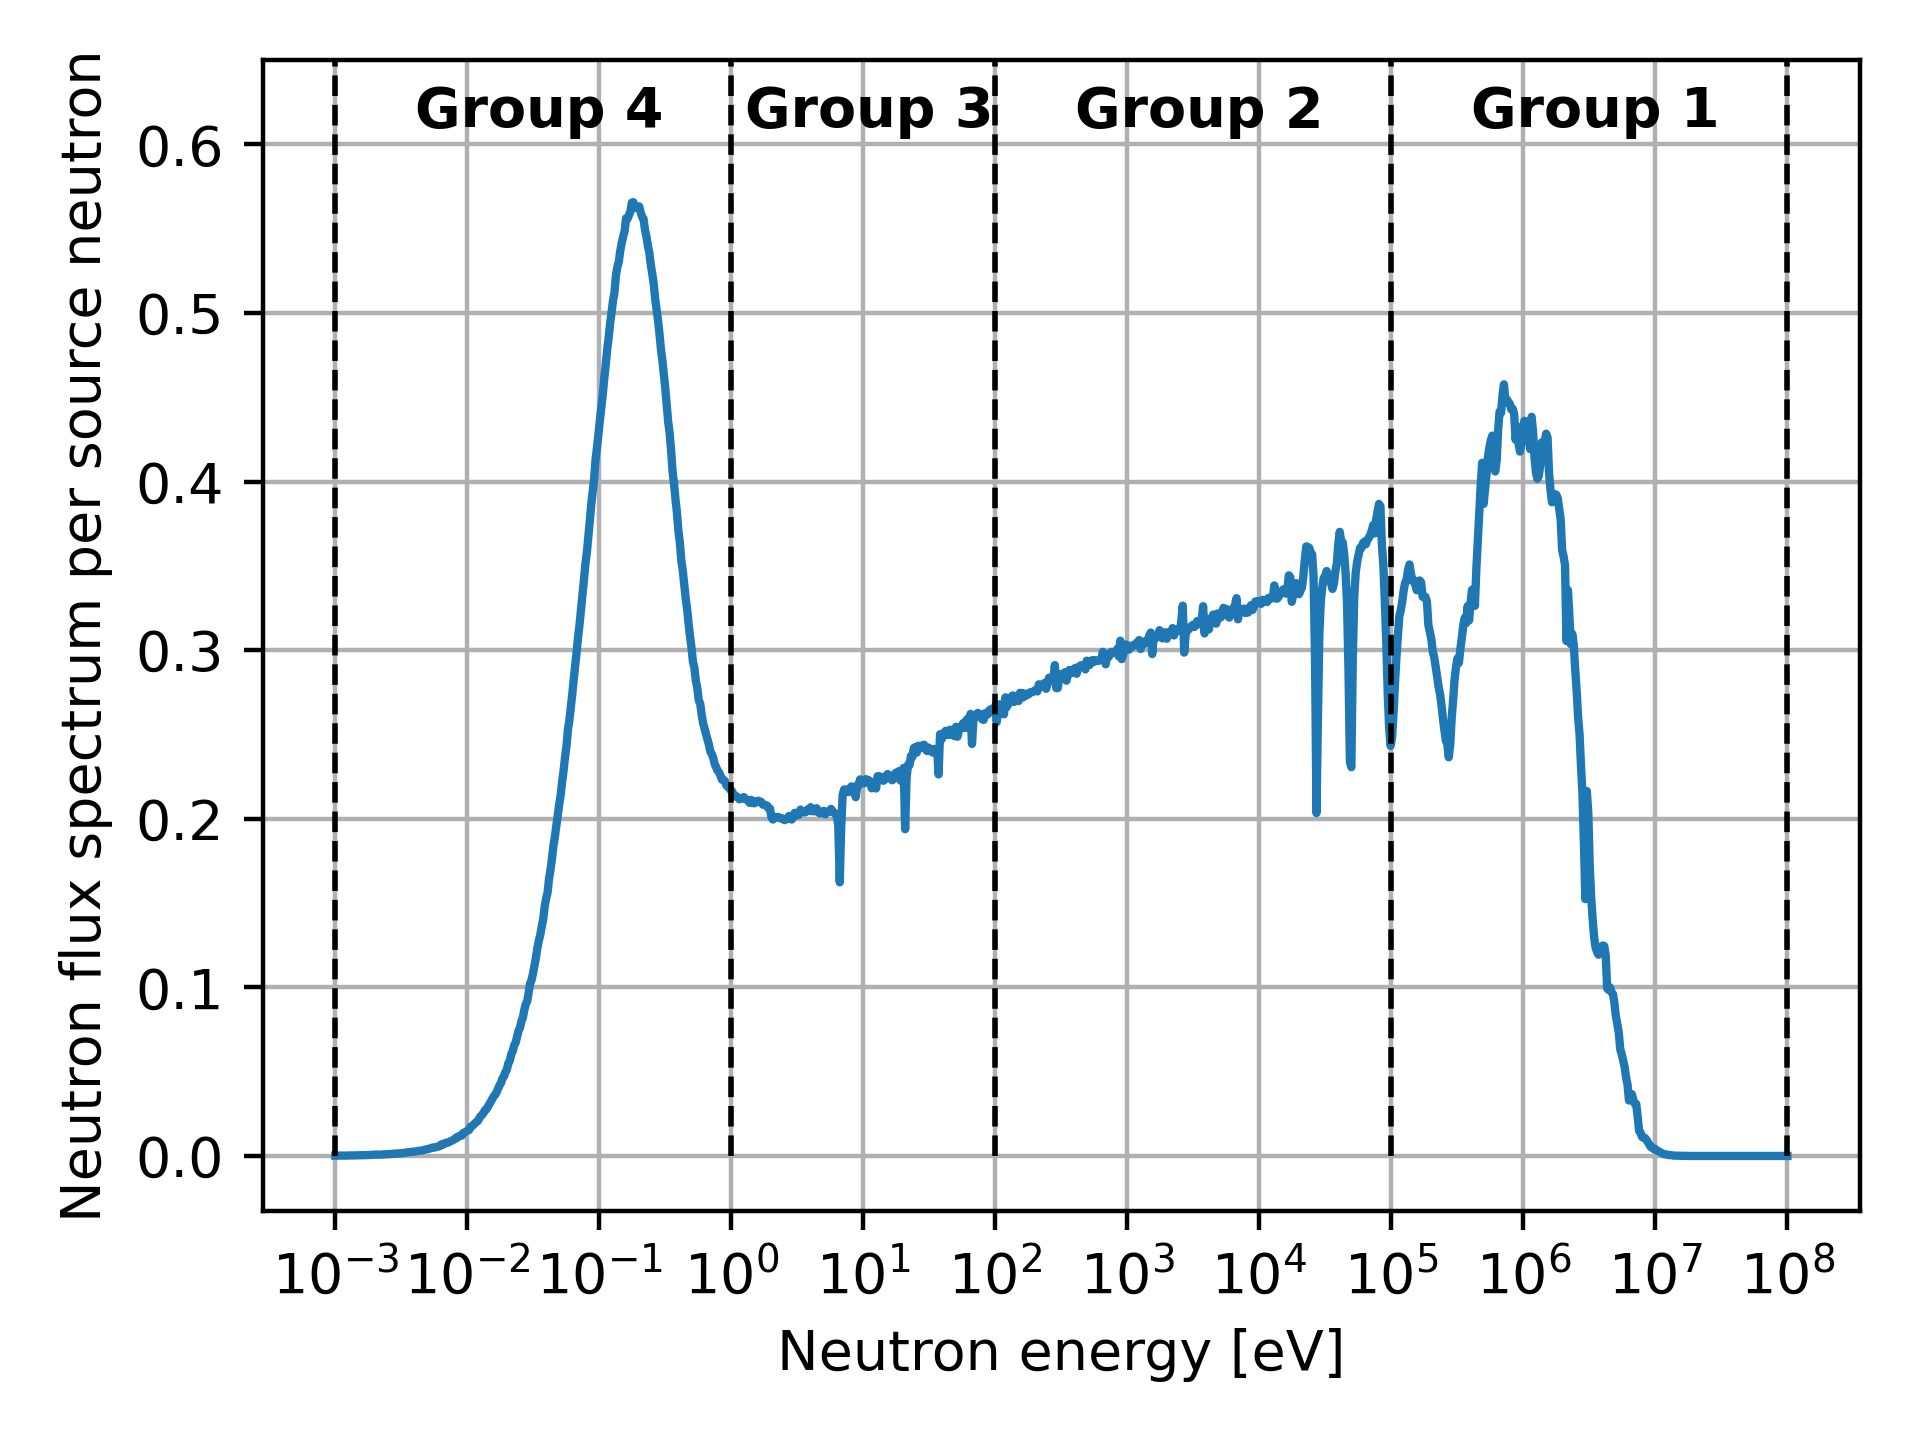
\includegraphics[width=\textwidth]{spectrum}
    \caption{Neutron flux energy spectrum per source neutron}
    \label{fig:spectrum}
  \end{subfigure}
  \hfill
  \begin{subfigure}[t]{.49\textwidth}
    \centering
    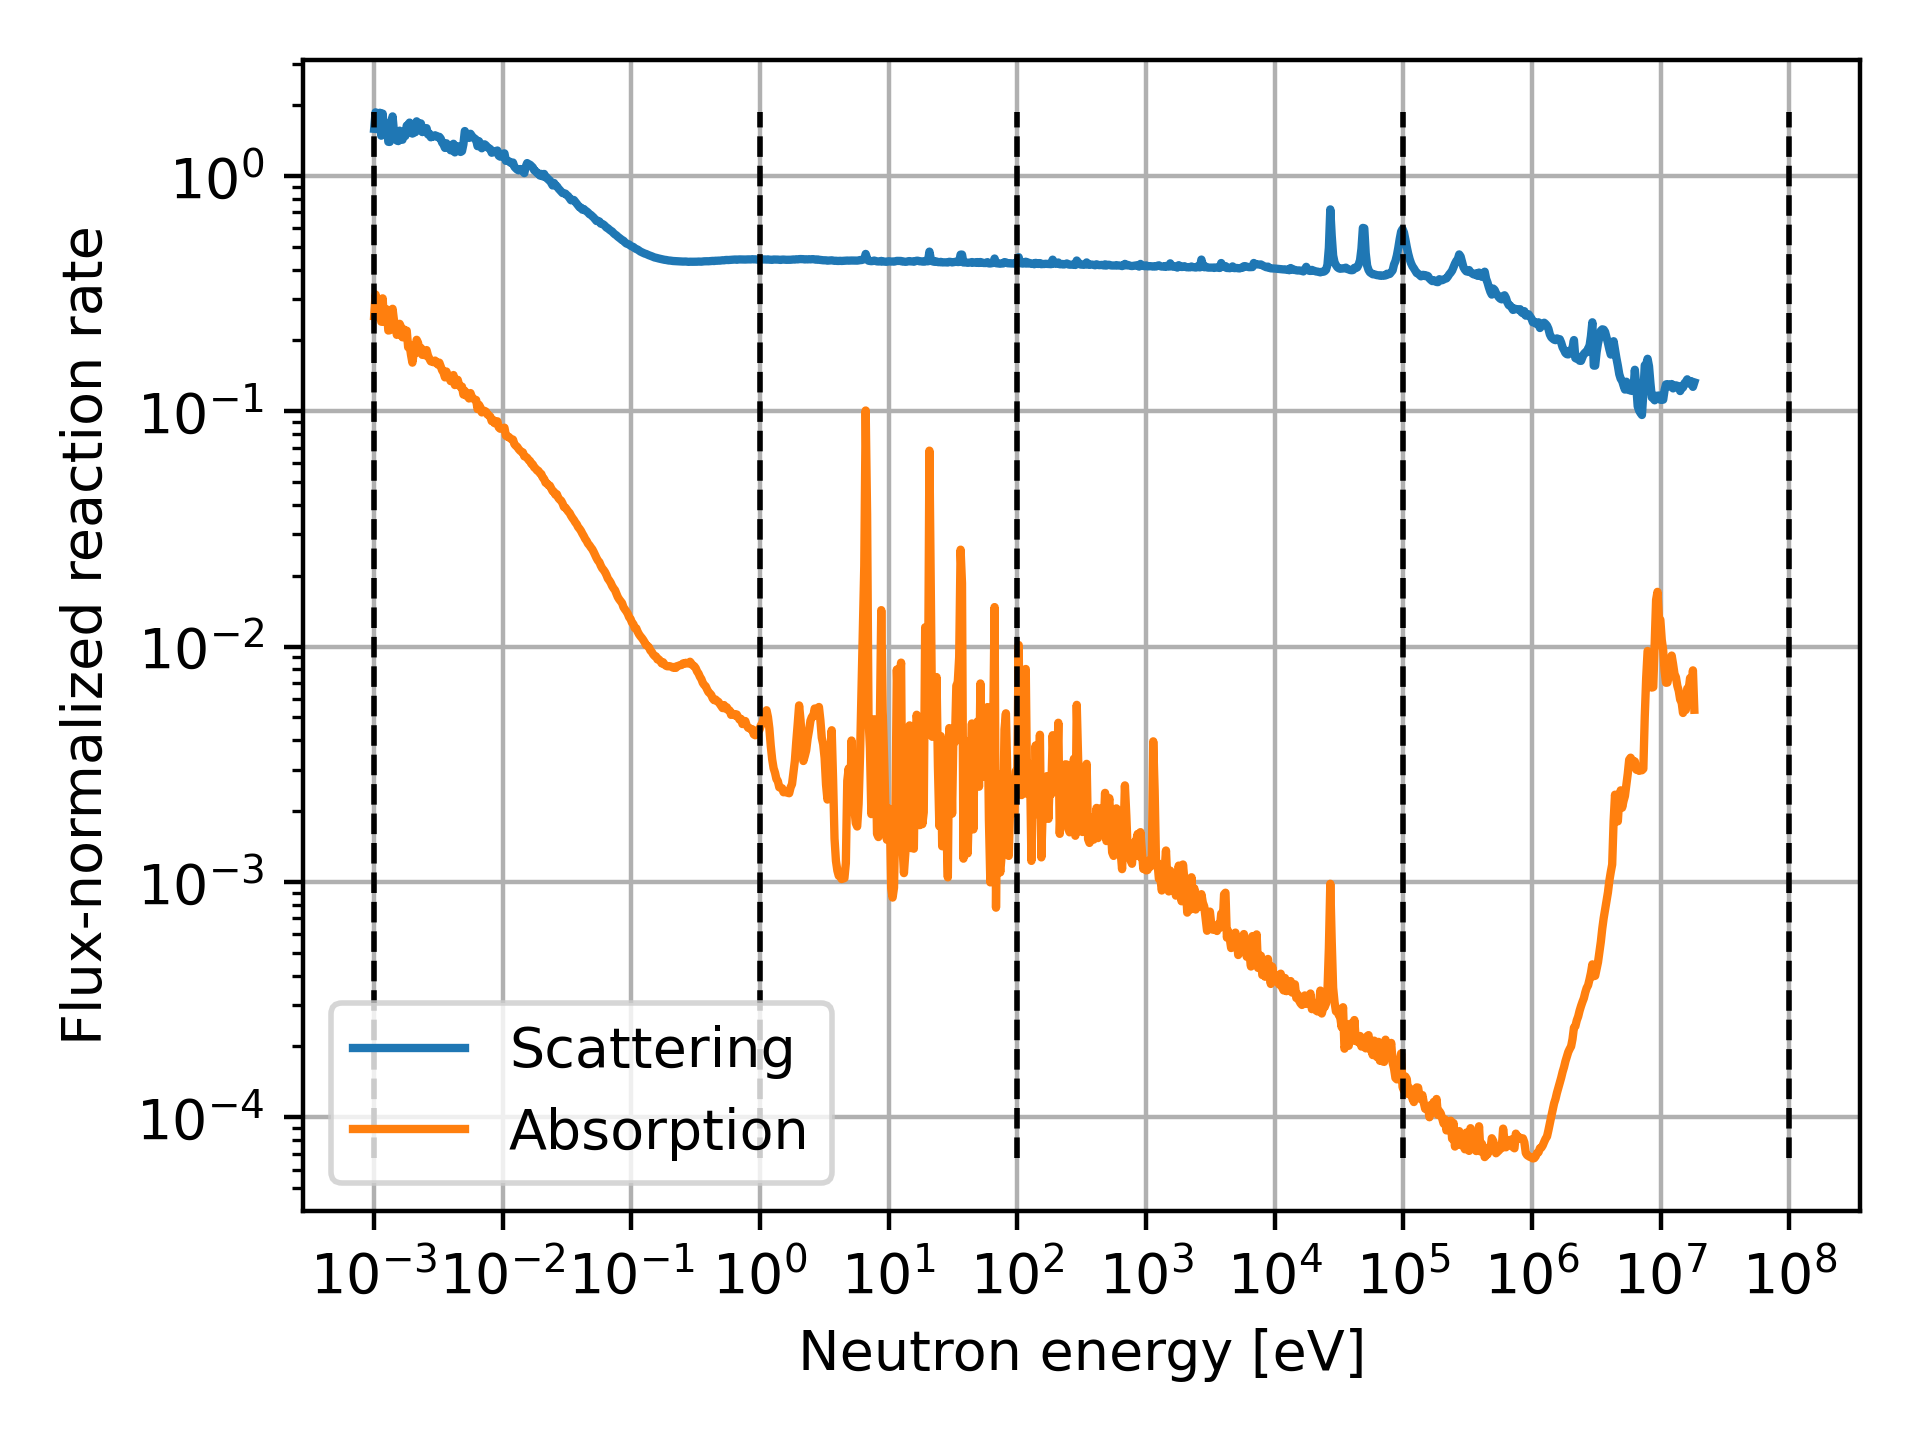
\includegraphics[width=\textwidth]{reaction}
    \caption{Flux-normalized scattering and absorption reaction rates}
    \label{fig:reaction}
  \end{subfigure}
  \caption{Neutron flux energy spectrum and reaction rates for Case 5a. The dotted vertical lines
  correspond to the discrete neutron energy group boundaries.}
  \label{fig:spec-reac}
\end{figure}
%
%\begin{table}[tb!]
%  \centering
%  \caption{Description of the 1-D Test Case Geometries.}
%  \begin{tabular}{l c c c}
%    \toprule
%    Cases & Ordered list of regions & Ordered list of interface x-coordinates & Left \& Right BCs\\
%    \midrule
%    Case 0 & Control rod, homogenized fuel-graphite lattice &
%    \bottomrule
%  \end{tabular}
%  \label{table:c0k}
%\end{table}

I ran all cases with four neutron energy groups bounded at $E=10^{-5}, 10^0, 10^2, 10^5, 10^8$
eV. Figures \ref{fig:spectrum} and \ref{fig:reaction} show how this energy group structure
partitions the neutron flux energy spectrum and neutron reaction rates. For this preliminary work,
the four-group structure is sufficient for showing different scattering and absorption trends of
slow, intermediate, and fast neutrons. I also ran all cases on OpenMC to generate the required
group constants and to assess the accuracy of the deterministic methods against OpenMC in
continuous-energy (OpenMC-CE) and multigroup (OpenMC-MG) modes. Table \ref{table:var} shows how the
position, direction of travel, neutron energy, and angle-dependence in $\Sigma_s$ are handled by
OpenMC and the deterministic methods. Comparing OpenMC-MG results with OpenMC-CE results allows us
to quantify errors arising from neutron energy group discretization and the scattering cross
section simplifications. Each Monte Carlo simulation ran on 25 inactive and 125 active cycles of
20,000 neutrons each, which sums up to 2.5 million tallied neutron histories.

\begin{table}[tb!]
  \centering
  \footnotesize
  \caption{Variable handling in OpenMC under continuous-energy (OpenMC-CE) and multigroup
  (OpenMC-MG) modes, and in the $S_N$ neutron transport, neutron diffusion, and Hybrid
  $S_N$-Diffusion methods. }
  \begin{tabular}{c c c c c c}
    \toprule
    Variable & OpenMC-CE & OpenMC-MG & $S_N$ Transport & Diffusion & Hybrid \\
    \midrule
    Position, $\bm{r}$ & Continuous & Continuous & Discrete & Discrete & Discrete \\
    Direction of travel, $\bm{\hat{\Omega}}$ & Continuous & Continuous & Discrete & N/A & N/A \\
    Energy, $E$ & Continuous & Discrete & Discrete & Discrete & Discrete \\
    Angle-dependence in $\Sigma_s$ & Continuous & 2nd Legendre moment & 2nd Legendre moment
    & N/A & N/A \\
    \bottomrule
  \end{tabular}
  \label{table:var}
\end{table}

\section{Simulation Parameters for Convergence} \label{sec:sim-param}

The convergence of the results depends mainly on the following simulation parameters: mesh size
($\Delta x$), convergence tolerance ($tol$), number of discrete ordinates ($N$), and the highest
order moment of the scattering cross sections ($L$). The last two parameters apply only to $S_N$
calculations. Table \ref{table:param} shows the values of simulation parameters applied to each
method for the 1-D test cases.

\begin{table}[tb!]
  \centering
  \footnotesize
  \caption{Simulation parameters applied to the neutron diffusion, $S_N$, and Hybrid
  $S_N$-Diffusion methods.}
  \begin{tabular}{c c c c}
    \toprule
    Parameter & $S_N$ Transport & Neutron Diffusion & Hybrid $S_N$-Diffusion \\
    \midrule
    Mesh size, $\Delta x$ [cm]        & 0.0125    & 0.0125    & 0.0125 \\[.2cm]
    \multirow{3}{*}{Convergence tolerance, $tol$}
                                      &           &           & Diffusion: $10^{-6}$ \\
                                      & $10^{-7}$ & $10^{-6}$ & $S_N$: $10^{-5}$ \\
                                      &           &           & Outer: $10^{-3}$ \\[.2cm]
    Discrete ordinates, $N$           & 8         & N/A       & 8 \\
    Highest moment of $\Sigma^{g'\rightarrow g}_s$, $L$
                                      & 2         & N/A       & 2 \\
    \bottomrule
  \end{tabular}
  \label{table:param}
\end{table}

The simulation parameters did not show any significant correlation in the convergence tests. All
three methods achieve reasonable convergence with $\Delta x=0.0125$ cm; halving the mesh size
causes less than $30\times10^{-5}$ change in $k$ for the neutron diffusion and hybrid methods and
less than $10^{-5}$ for the $S_8$ method. Further refinement of the $tol$, $N$, and $L$ parameters
result in less than $2\times10^{-5}$
change in $k$. The same $tol$ value applies to convergence checks for both $\phi$ and $k$ in all
three methods because the variables converge at similar rates. The hybrid method requires three
separate $tol$ values due to the inner and outer iterations. Notably, the hybrid method can reach
convergence with a larger $tol$ value for its $S_N$ subsolver than the $tol$ value for the
standalone $S_N$ solver, which implies that $J$ and $\sfrac{d\phi}{dx}$ converge faster than $\phi$
because the \glspl{SVDC} depend on those variables instead of $\phi$. Consequently, the $S_N$
subsolver requires much fewer iterations than the standalone $S_N$ solver. In combination with
restricting $S_N$ calculations to the correction region, the hybrid method saves significant
computation time compared to the standalone $S_N$ method.

The outer iterations
converge rapidly, so a $tol$ value of $10^{-3}$ is sufficient for convergence. The $\phi$ and $k$
relative error norms ($\epsilon$) in all test cases decreased by two orders of magnitude on
every outer iteration. For instance, Table \ref{table:epsilon} shows the $\epsilon$ values from the
hybrid method after every outer iteration for Case 5a. The $epsilon$ values fall below
$10^{-5}$ by the 3rd and 4th iterations.

\begin{table}[tb!]
  \centering
  \footnotesize
  \caption{Relative error norm, $\epsilon$, values for $k$ and $\phi$ after each outer iteration in
    the Hybrid $S_N$-Diffusion method for Case 5a.}
  \begin{tabular}{c S[table-format=1.1e+1] S[table-format=1.1e+1]}
    \toprule
    Iteration   & {$\epsilon_k$}    & {$\epsilon_\phi$} \\
    \midrule
    1           & 1.6e-2            & 1.5e-2 \\
    2           & 5.0e-5            & 4.7e-5 \\
    3           & 1.4e-7            & 1.6e-7 \\
    4           & 3.5e-9            & 1.4e-8 \\
    \bottomrule
  \end{tabular}
  \label{table:epsilon}
\end{table}


\section{Results \& Discussion} \label{sec:prelim-results}

In this section, I will compare neutronics parameters for all test cases calculated from
the OpenMC and deterministic methods. I refer to the OpenMC calculations under continuous-energy
and multigroup modes as OpenMC-CE and OpenMC-MG, respectively.

\subsection{Comparison of Multiplication factors, $k$}

Tables \ref{table:ck1} and \ref{table:ck2} show all test case $k$ estimates from the OpenMC and
deterministic methods. The tables also include statistical uncertainties for the OpenMC
$k$ estimates. I did not apply the hybrid method for cases that do not contain control rod
regions. 

All five methods generally show reasonable agreement within each test case. The differences between
the OpenMC-CE and OpenMC-MG $k$ estimates vary significantly from 0.00018 in Case 1a to 0.01622 in
Case 4b. These Monte Carlo methods exhibit more significant differences in cases
with vacuum boundary conditions (e.g., Cases 1b, 2b, 3b, 4b, 5a, 5b). These differences imply that
the neutron energy discretization scheme must be revised to capture neutron leakage rates
accurately. Beyond this preliminary study, I will explore better discrete energy group structures
for further neutronics analyses of graphite-moderated \glspl{MSR}. For the rest of this
section, I compare the $k$ estimates of the deterministic methods with OpenMC-MG.

\begin{table}[htb!]
  \centering
  \footnotesize
  \caption{Multiplication factor $k$ estimates for Cases 1a, 1b, 2a, 2b, 3a, and 3b from the
    OpenMC-CE, OpenMC-MG, $S_8$ neutron transport, neutron diffusion, and Hybrid $S_N$-Diffusion
    methods.}
  \begin{tabular}{c S[table-format=1.5(2)] S[table-format=1.5(2)] S[table-format=1.5(2)]
  S[table-format=1.5(2)] S[table-format=1.5(2)] S[table-format=1.5(2)]}
    \toprule
    \multirow{2}{*}{\textbf{Method}} &
    \multicolumn{6}{c}{\textbf{Multiplication factor,} $\bm{k}$} \\
    \cmidrule{2-7}
    & {\textbf{Case 1a}} & {\textbf{Case 1b}} & {\textbf{Case 2a}} &
    {\textbf{Case 2b}} & {\textbf{Case 3a}} & {\textbf{Case 3b}} \\
    \midrule
    OpenMC-CE & 1.60033(56) & 1.16749(60) & 1.20666(66) & 0.69499(47) & 1.19908(63) & 0.68565(53)\\
    OpenMC-MG & 1.60015(33) & 1.18104(54) & 1.20570(66) & 0.70539(50) & 1.19976(48) & 0.69730(50)\\
    $S_8$     & 1.60035     & 1.18068     & 1.20596     & 0.70470     & 1.19968     & 0.69652    \\
    Diffusion & 1.60036     & 1.17932     & 1.19709     & 0.69274     & 1.19064     & 0.68450    \\
    Hybrid    & {N/A}       & {N/A}       & 1.20630     & 0.70387     & 1.20004     & 0.69568    \\
    \bottomrule
  \end{tabular}
  \label{table:ck1}
\end{table}
%
\begin{table}[htb!]
  \centering
  \footnotesize
  \caption{Multiplication factor $k$ estimates for Cases 4a, 4b, 5a, and 5b from the OpenMC-CE,
    OpenMC-MG, $S_8$ neutron transport, neutron diffusion, and Hybrid $S_N$-Diffusion methods.}
  \begin{tabular}{c S[table-format=1.5(2)] S[table-format=1.5(2)] S[table-format=1.5(2)]
    S[table-format=1.5(2)]}
    \toprule
    \multirow{2}{*}{\textbf{Method}} &
    \multicolumn{4}{c}{\textbf{Multiplication factor,} $\bm{k}$} \\
    \cmidrule{2-5}
    & {\textbf{Case 4a}} & {\textbf{Case 4b}} & {\textbf{Case 5a}} &
    {\textbf{Case 5b}} \\
    \midrule
    OpenMC-CE & 1.64506(53) & 1.19116(63) & 0.70352(64) & 1.16832(58) \\
    OpenMC-MG & 1.64355(37) & 1.20738(63) & 0.71396(50) & 1.18204(53) \\
    $S_8$     & 1.64376     & 1.20744     & 0.71379     & 1.18218     \\
    Diffusion & 1.64355     & 1.20811     & 0.70524     & 1.18274     \\
    Hybrid    & {N/A}       & {N/A}       & 0.71673     & {N/A}       \\
    \bottomrule
  \end{tabular}
  \label{table:ck2}
\end{table}
%
\begin{table}[htb!]
  \centering
  \footnotesize
  \caption{Differences in $k$ estimates for Cases 1a, 1b, 2a, 2b, 3a, and 3b for the $S_8$ neutron
    transport, neutron diffusion, and Hybrid $S_N$-Diffusion methods relative to OpenMC-MG.}
  \begin{tabular}{c S[table-format=+1.5(2)] S[table-format=+1.5(2)] S[table-format=+1.5(2)]
      S[table-format=+1.5(2)] S[table-format=+1.5(2)] S[table-format=+1.5(2)]}
    \toprule
    \multirow{2}{*}{\textbf{Method}} & \multicolumn{6}{c}{$\bm{k-k_{MG}}$} \\
    \cmidrule{2-7}
    & {\textbf{Case 1a}} & {\textbf{Case 1b}} & {\textbf{Case 2a}} &
    {\textbf{Case 2b}} & {\textbf{Case 3a}} & {\textbf{Case 3b}} \\
    \midrule
    $S_8$     & +0.00020(33) & -0.00036(54) & +0.00026(66) & -0.00069(50) & -0.00008(48) & -0.00078(50) \\
    Diffusion & +0.00021(33) & -0.00172(54) & -0.00861(66) & -0.01265(50) & -0.00912(48) & -0.01280(50) \\
    Hybrid    & {N/A}        & {N/A}        & +0.00060(66) & -0.00152(50) & +0.00028(48) & -0.00162(50) \\
    \bottomrule
  \end{tabular}
  \label{table:ckdiff1}
\end{table}
%
\begin{table}[htb!]
  \centering
  \footnotesize
  \caption{Differences in $k$ estimates for Cases 4a, 4b, 5a, and 5b for the $S_8$ neutron
    transport, neutron diffusion, and Hybrid $S_N$-Diffusion methods relative to OpenMC-MG.}
  \begin{tabular}{c S[table-format=+1.5(2)] S[table-format=+1.5(2)] S[table-format=+1.5(2)]
    S[table-format=+1.5(2)]}
    \toprule
    \multirow{2}{*}{\textbf{Method}} & \multicolumn{4}{c}{$\bm{k-k_{MG}}$} \\
    \cmidrule{2-5}
    & {\textbf{Case 4a}} & {\textbf{Case 4b}} & {\textbf{Case 5a}} &
    {\textbf{Case 5b}} \\
    \midrule
    $S_8$     & +0.00021(37) & +0.00006(63) & -0.00017(50) & -0.00027(53) \\
    Diffusion & +0.00000(37) & +0.00073(63) & -0.00872(50) & +0.00277(53) \\
    Hybrid    & {N/A}        & {N/A}        & +0.00070(50) & {N/A}    \\
    \bottomrule
  \end{tabular}
  \label{table:ckdiff2}
\end{table}
%
\begin{table}[tb!]
  \centering
  \footnotesize
  \caption{Control rod worths calculated as changes in the reactivity between Case 5a and 5b for
    the OpenMC continuous-energy and multigroup mode calculations, and the $S_8$ neutron transport,
  neutron diffusion, and Hybrid $S_N$-Diffusion methods.}
  \begin{tabular}{c S}
    \toprule
    \multirow{2}{*}{\textbf{Method}} & {\textbf{Control rod worth}} \\
                                     & {$\bm{\rho_{(5b)}-\rho_{(5a)}}$} \\
    \midrule
    OpenMC-CE & 0.56549(213) \\
    OpenMC-MG & 0.55464(176) \\
    $S_8$     & 0.55507 \\
    Diffusion & 0.57246 \\
    Hybrid    & 0.54974 \\
    \bottomrule
  \end{tabular}
  \label{table:rod-worth}
\end{table}

Tables \ref{table:ckdiff1} and \ref{table:ckdiff2} show the differences in $k$ between OpenMC-MG
and deterministic methods. The $k$ estimates from the $S_8$ neutron transport method show
good agreement, with the estimates from OpenMC-MG with all pairs of $k$ values falling within
1-2 standard deviations of each other. The only significant difference in implementation between
the OpenMC-MG and $S_8$ methods is the discretization of the direction of travel variable
$\hat{\Omega}$. The flux distributions exhibit more apparent differences, will be discussed in the
following subsection. Nevertheless, the $S_8$ method is sufficiently accurate and consistent for
modeling this graphite-moderated system with control rods.

As expected, the neutron diffusion method performs significantly worse than the $S_8$ method in
Cases 2, 3, and 5a, containing control rod regions. It deviates from the OpenMC-MG $k$
estimate by up to -0.01280 in Case 3b compared to -0.00078 for the $S_8$ method. The hybrid method
effectively improves the $k$ estimate to -0.00162 of the
OpenMC-MG method for Case 3b. The hybrid method also appreciably improved the accuracy in all
other applied cases.

The control rod worth is the most crucial parameter for assessing the suitability of the
hybrid method for modeling control rods. In a time-dependent multiphysics simulation involving rod
insertion or withdrawal, the control rod worth determines the change in reactivity and the
subsequent effects on the neutron flux and temperature distribution. I calculated the control rod
worth by taking the change in reactivity $\rho$ between Case 5a and 5b for all five methods, as
shown in Table \ref{table:rod-worth}. The formula for $\rho$ is given as
%
\begin{align}
  \rho =& \frac{k-1}{k}.
\end{align}
%
I took the $k$ estimate from the neutron diffusion method in Case 5b as the reference non-inserted
case for the control rod worth calculation for the hybrid method. Compared with OpenMC-MG, the
control rod worth from the neutron diffusion method deviates the most by 1782 pcm (percent mille)
as opposed to 43 pcm and -490 pcm by the $S_8$ and hybrid methods, respectively.

\subsection{Comparison of Neutron Flux Distributions, $\phi$}

This section focuses on the neutron flux distributions in Cases 3b and 5a, representing the most
complex geometries with homogeneous and lattice fuel-graphite regions. I sampled the flux
distributions in OpenMC-CE and OpenMC-MG across coarser $0.1$-cm intervals to reduce the
statistical uncertainties of each flux reading.

\begin{figure}[htb!]
  \centering
  \begin{subfigure}[t]{.49\textwidth}
    \centering
    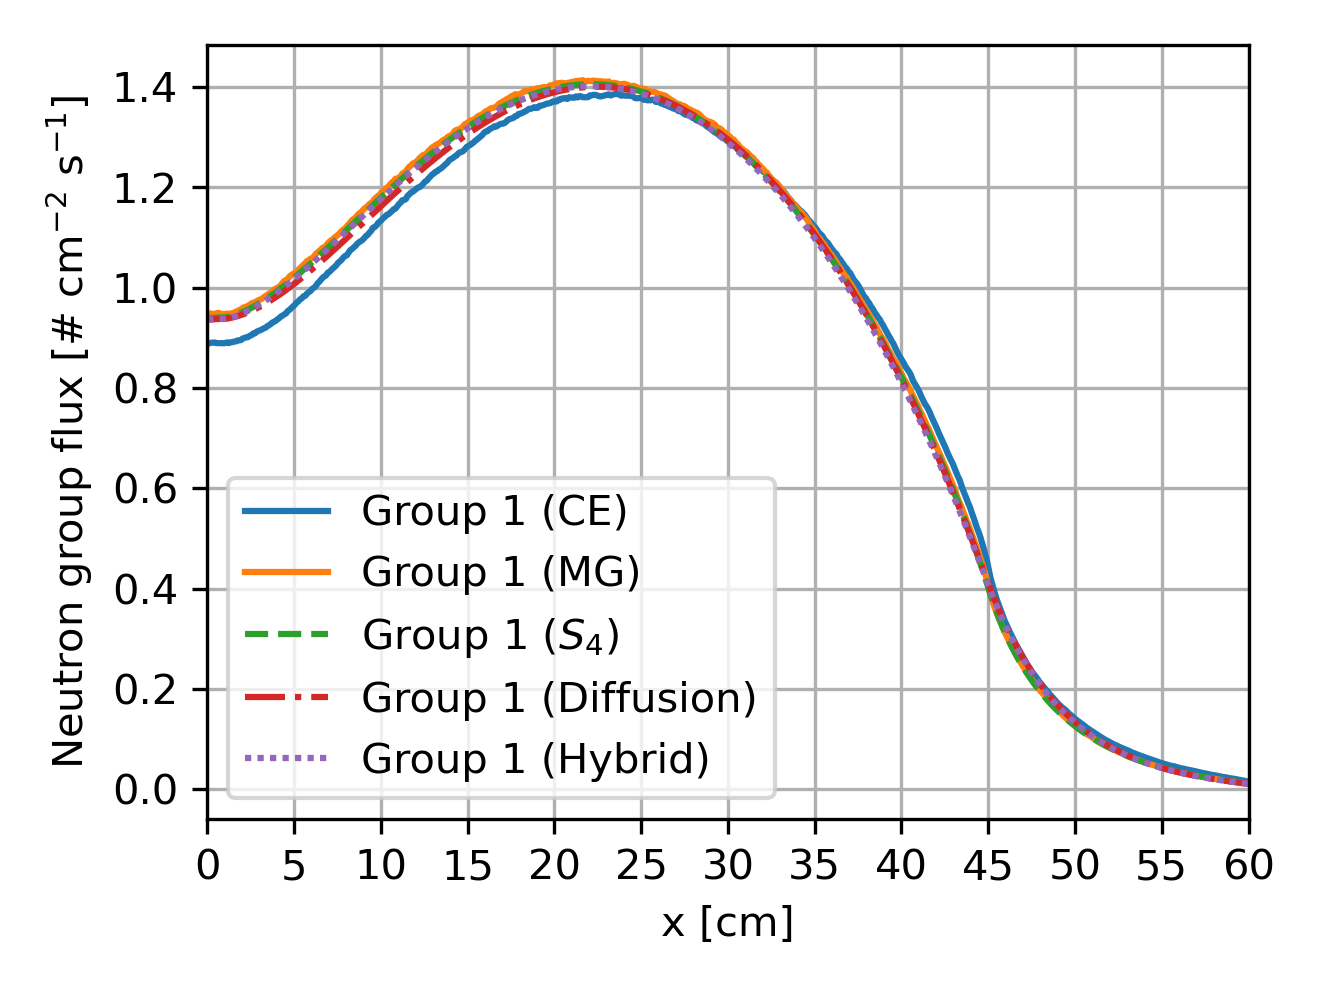
\includegraphics[width=\textwidth]{case-3b-group-1-flux}
    \caption{Group 1}
    \label{fig:c3bg1}
  \end{subfigure}
  \hfill
  \begin{subfigure}[t]{.49\textwidth}
    \centering
    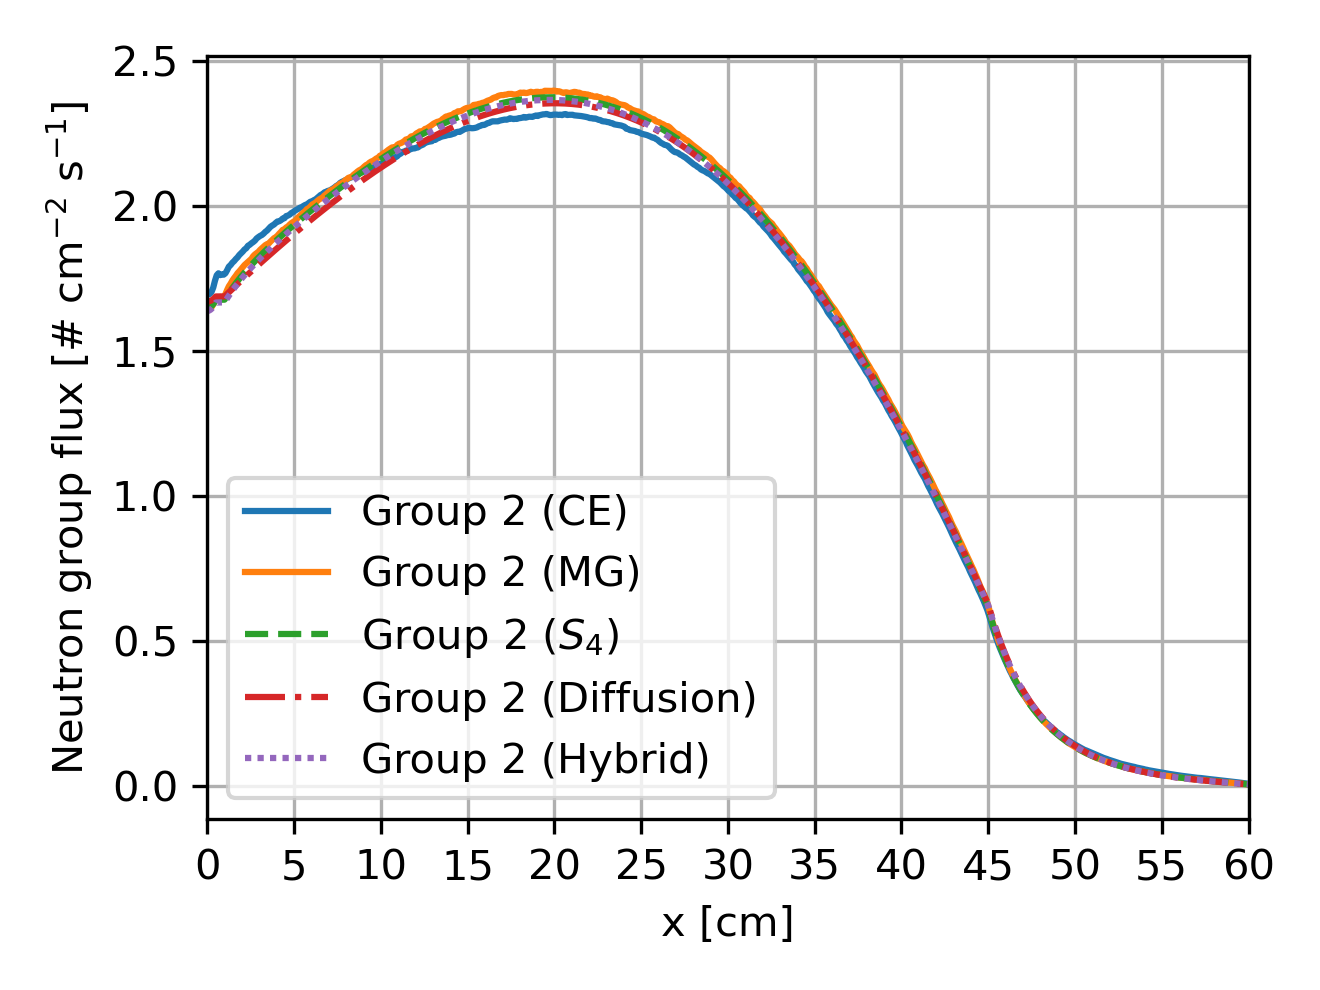
\includegraphics[width=\textwidth]{case-3b-group-2-flux}
    \caption{Group 2}
    \label{fig:c3bg2}
  \end{subfigure}
  \begin{subfigure}[t]{.49\textwidth}
    \centering
    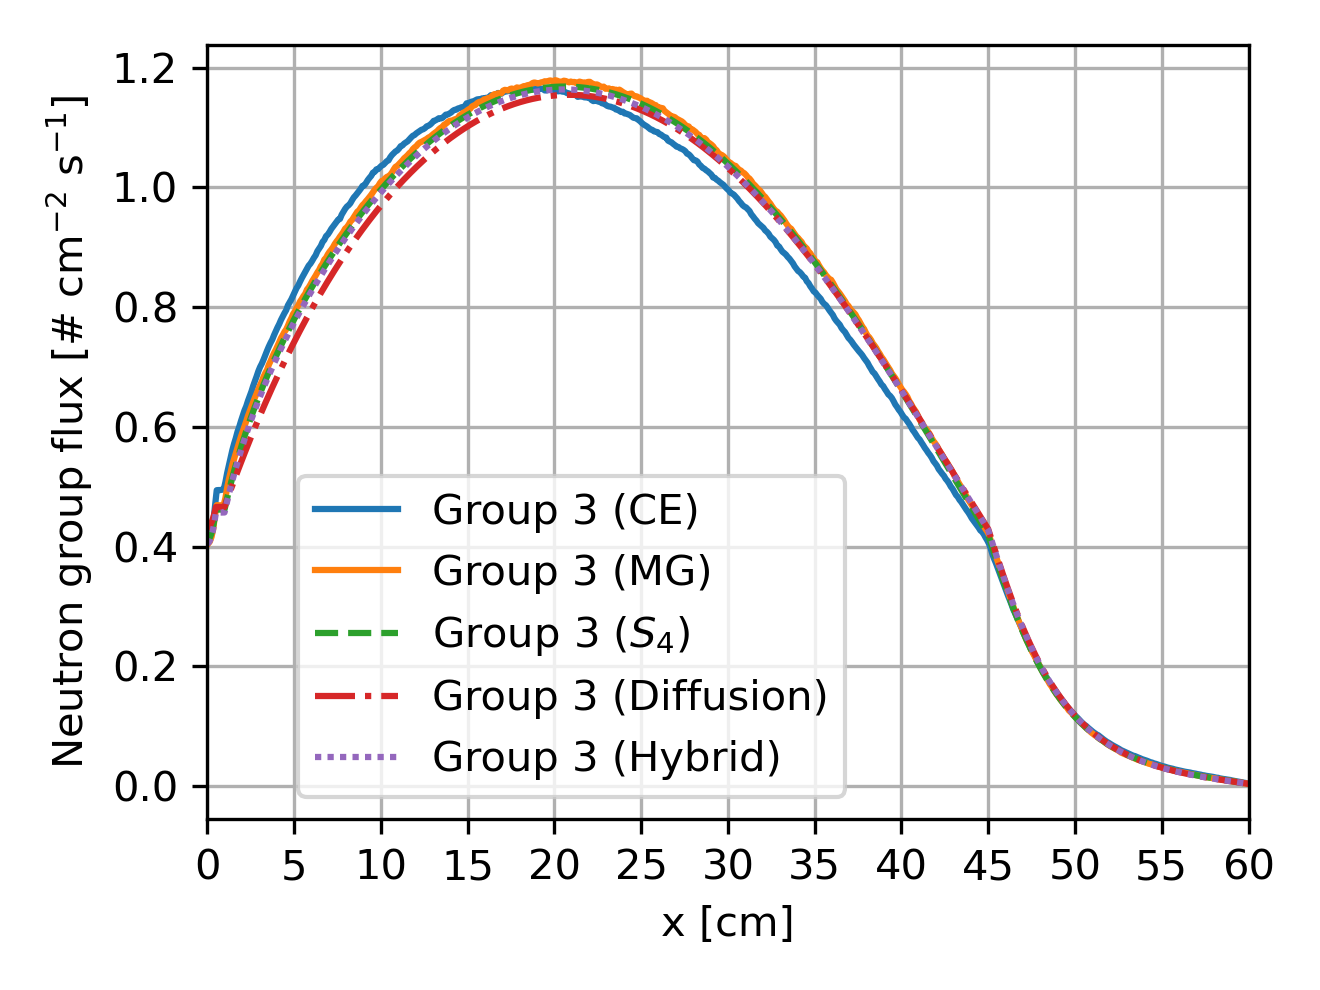
\includegraphics[width=\textwidth]{case-3b-group-3-flux}
    \caption{Group 3}
    \label{fig:c3bg3}
  \end{subfigure}
  \hfill
  \begin{subfigure}[t]{.49\textwidth}
    \centering
    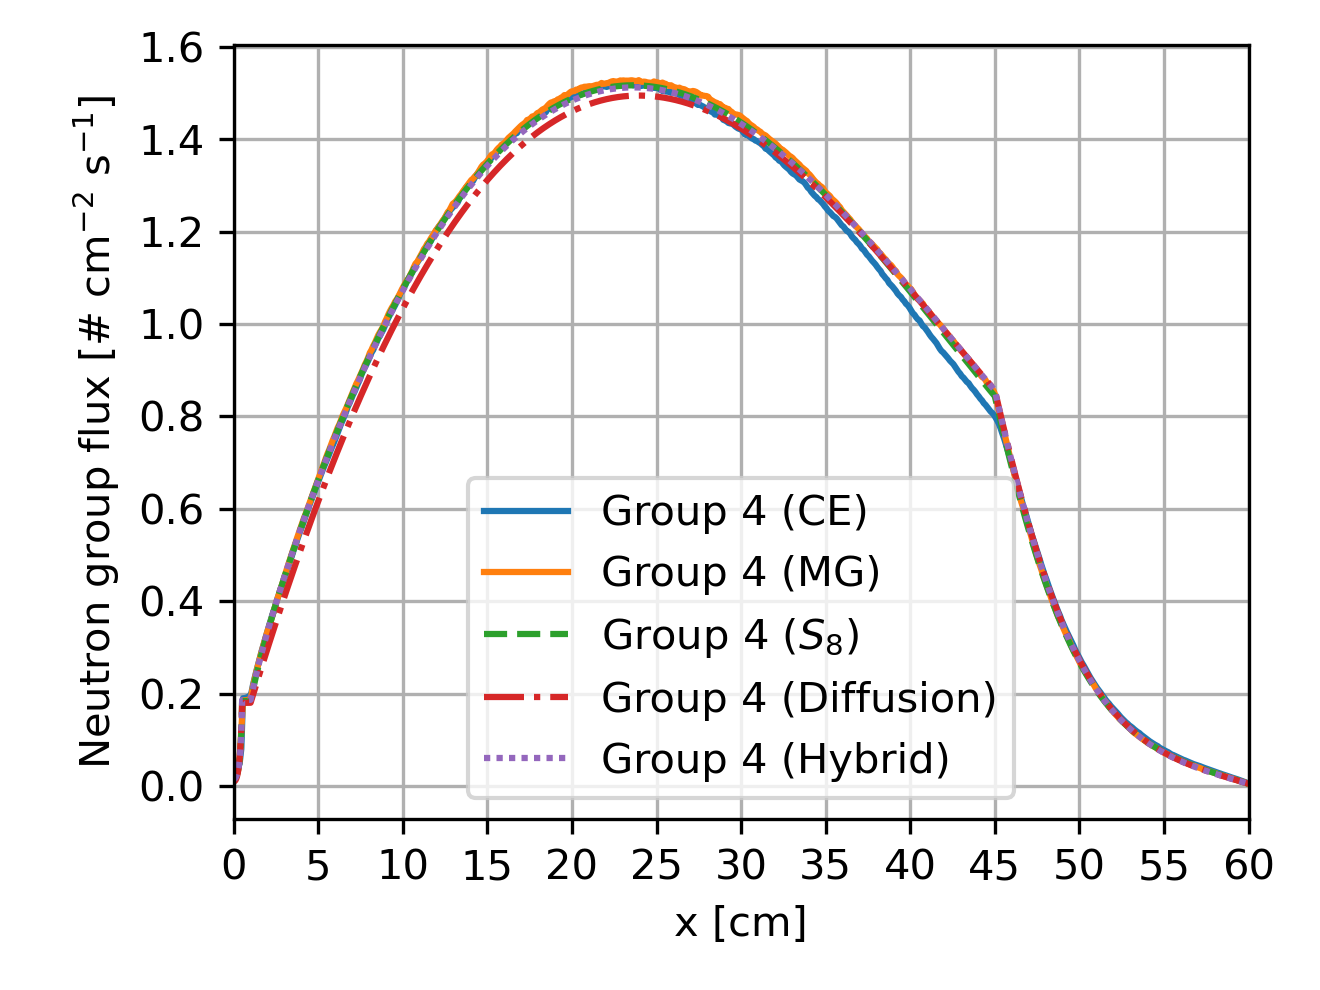
\includegraphics[width=\textwidth]{case-3b-group-4-flux}
    \caption{Group 4}
    \label{fig:c3bg4}
  \end{subfigure}
  \caption{Neutron group flux distributions for Case 3b from OpenMC-CE, OpenMC-MG, $S_8$, neutron
  diffusion, and hybrid methods.}
  \label{fig:c3bflux}
\end{figure}

Figure \ref{fig:c3bflux} shows the neutron flux distributions for groups 1 to 4. Notably, the
OpenMC-CE flux distribution is the most dissimilar, likely due to
the inadequate neutron energy discretization scheme. Consequently, I compared the
deterministic methods with OpenMC-MG to eliminate energy discretization errors. Figure
\ref{fig:c3bfluxe} shows the relative differences in the flux distributions from $S_8$, neutron
diffusion, and hybrid methods with respect to OpenMC-MG. The neutron diffusion method
performs worse than $S_8$, especially near the control rod region between $x=0$ cm and $x=20$ cm
for the slower group 3 and 4 neutron flux. Although the control rod region spans between $x=0$ cm
and $x=0.5$ cm only, it induces strong flux gradients in its vicinity, thus rendering the neutron
diffusion method less valid. The hybrid method significantly improves all four
group fluxes in this region. Beyond $x=40$ cm, the neutron diffusion and hybrid methods produce
similar flux error distributions due to the influence of the material interface between the
fuel-graphite and reflector regions.

\begin{figure}[htb!]
  \centering
  \begin{subfigure}[t]{.49\textwidth}
    \centering
    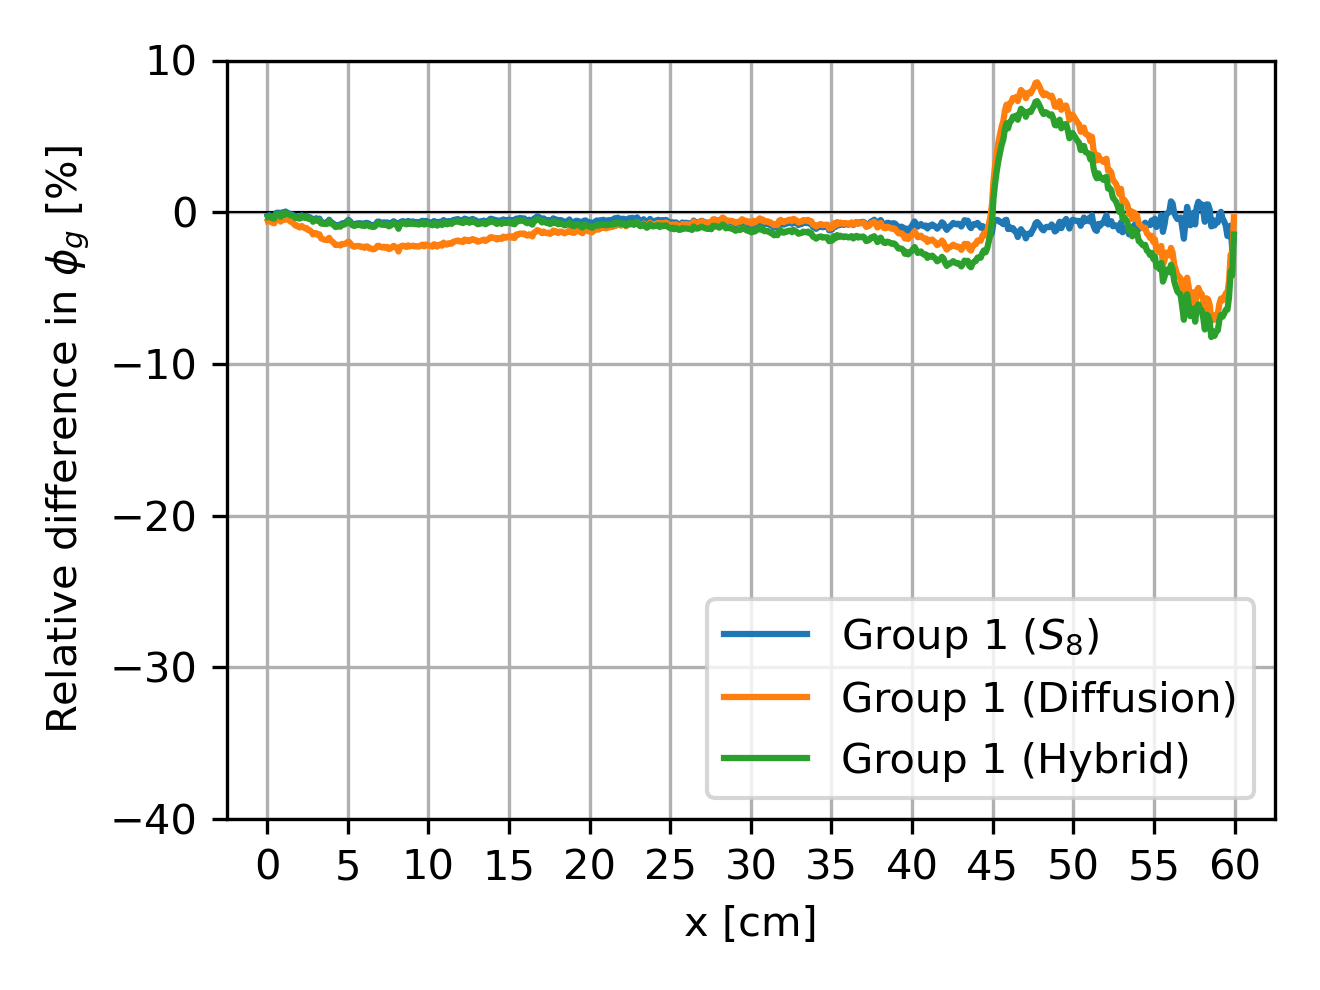
\includegraphics[width=\textwidth]{case-3b-group-1-flux-error}
    \caption{Group 1}
    \label{fig:c3bg1e}
  \end{subfigure}
  \hfill
  \begin{subfigure}[t]{.49\textwidth}
    \centering
    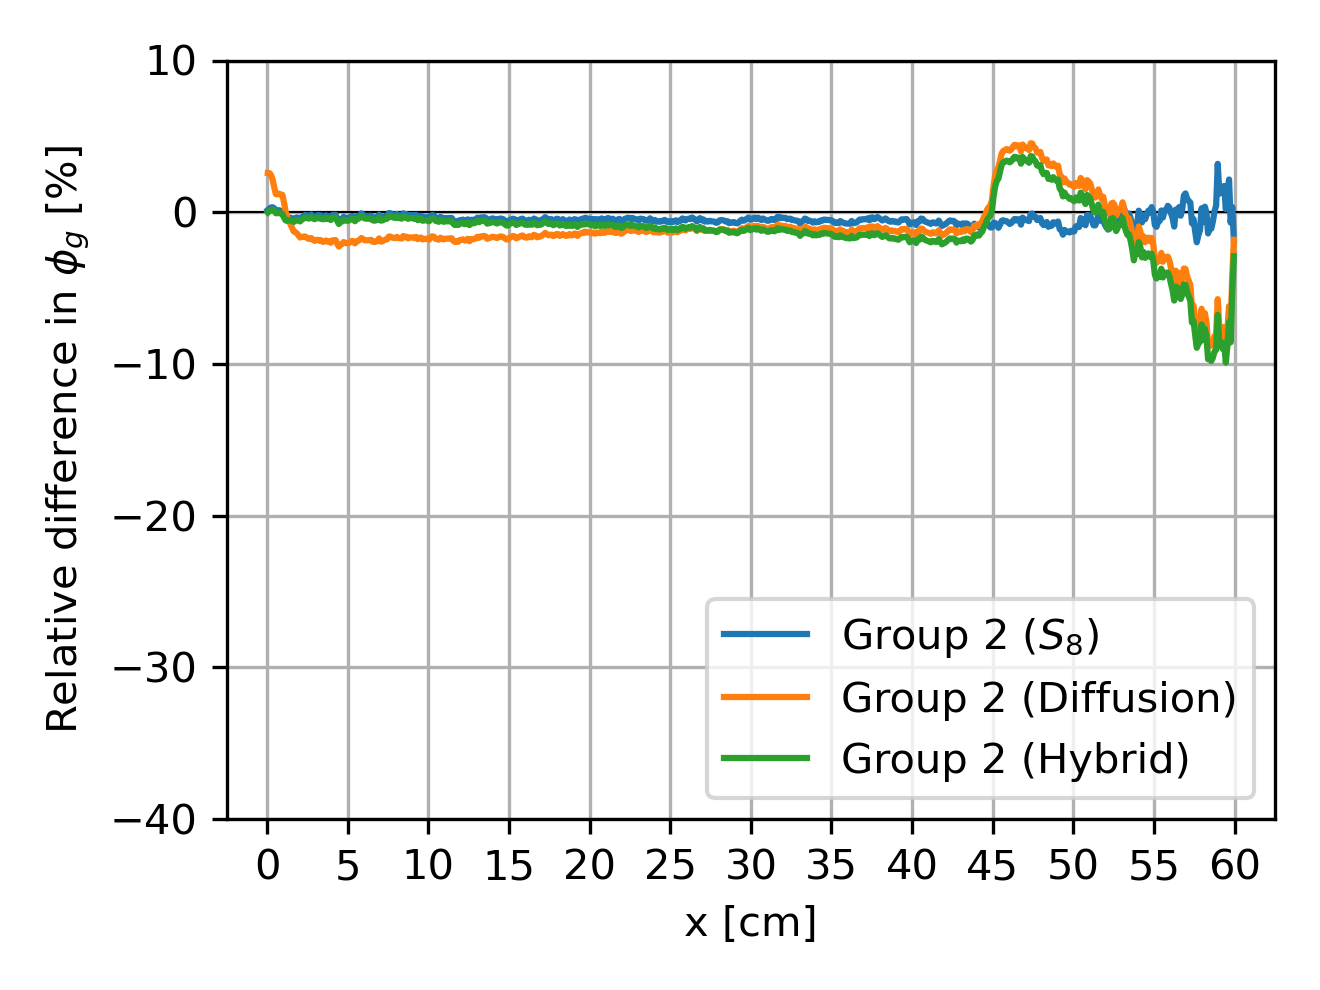
\includegraphics[width=\textwidth]{case-3b-group-2-flux-error}
    \caption{Group 2}
    \label{fig:c3bg2e}
  \end{subfigure}
  \begin{subfigure}[t]{.49\textwidth}
    \centering
    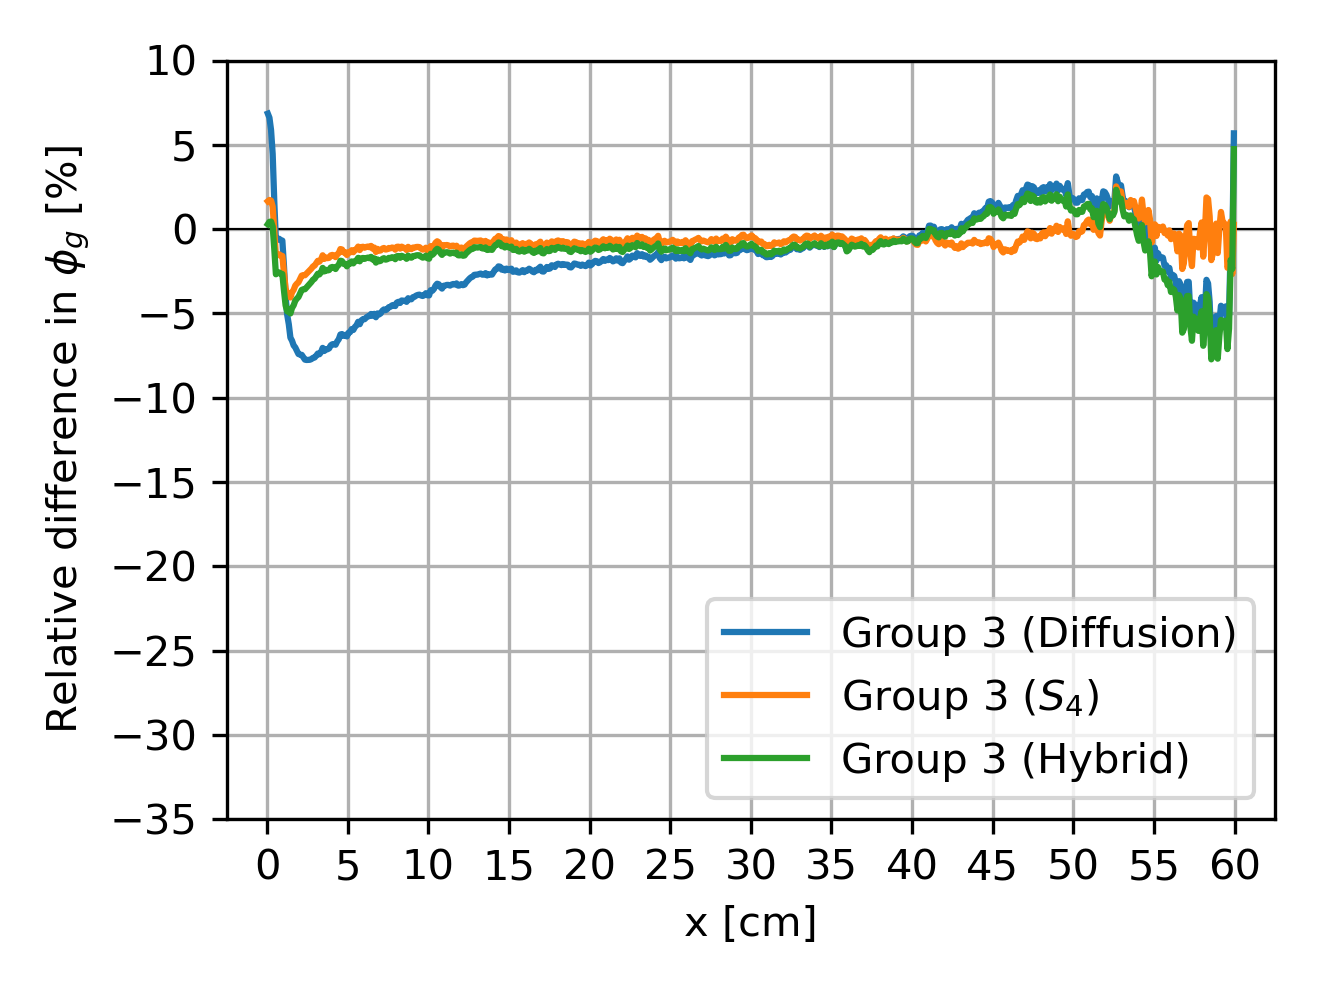
\includegraphics[width=\textwidth]{case-3b-group-3-flux-error}
    \caption{Group 3}
    \label{fig:c3bg3e}
  \end{subfigure}
  \hfill
  \begin{subfigure}[t]{.49\textwidth}
    \centering
    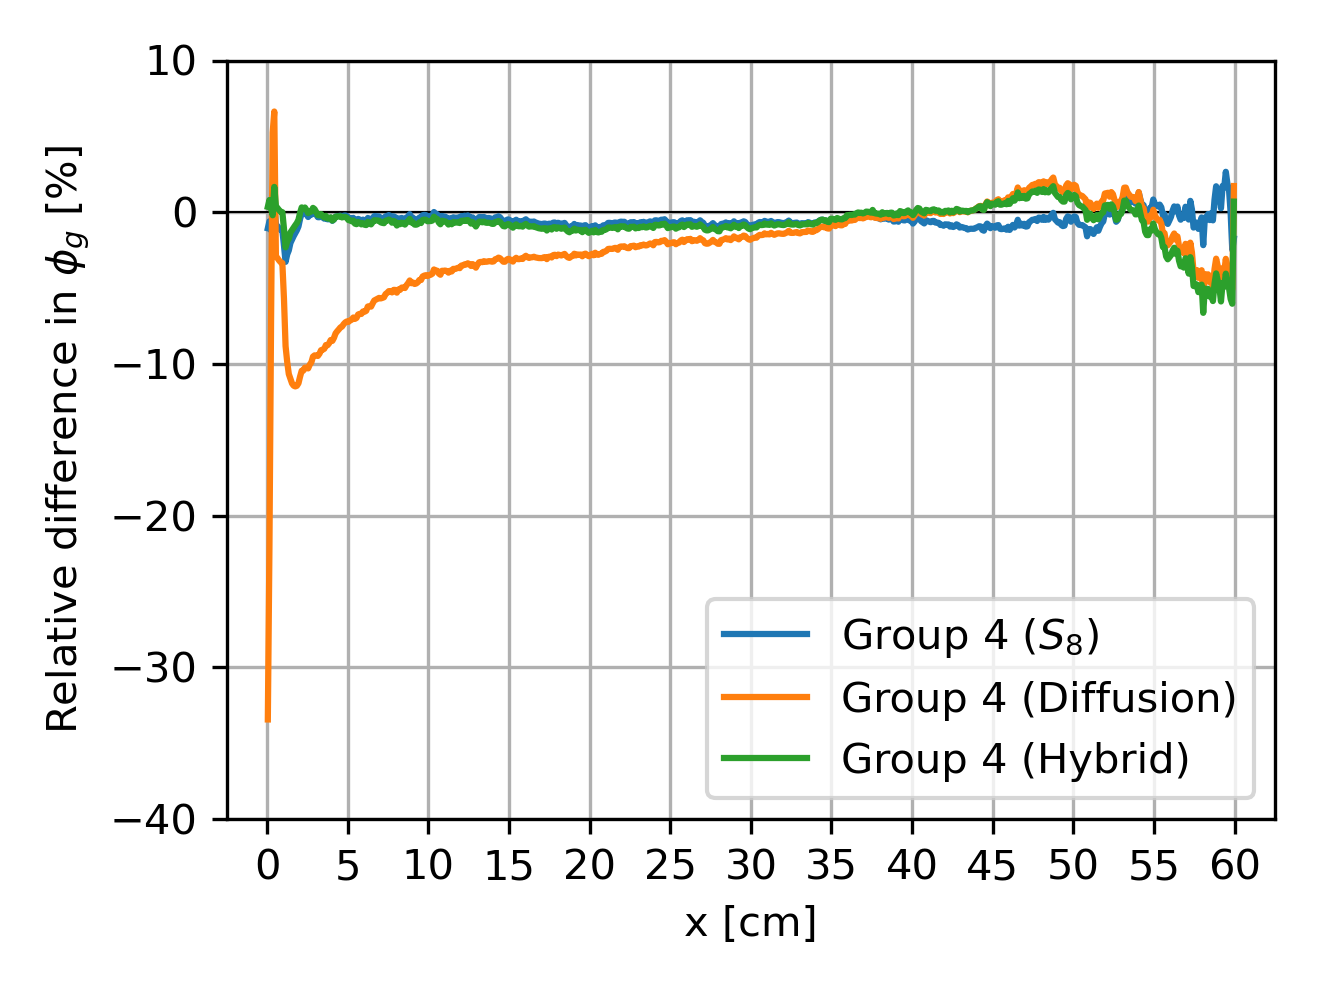
\includegraphics[width=\textwidth]{case-3b-group-4-flux-error}
    \caption{Group 4}
    \label{fig:c3bg4e}
  \end{subfigure}
  \caption{Relative differences of the neutron group flux distributions for Case 3b from the $S_8$,
    neutron diffusion, and hybrid methods with respect to OpenMC-MG.}
  \label{fig:c3bfluxe}
\end{figure}

For a quantitative assessment, I defined the normalized flux error $\varepsilon$ (not to be
confused with relative error norm $\epsilon$) for each energy group with respect to the OpenMC-MG
flux distribution using a normalized Frobenius/Euclidean norm formula given as
%
\begin{align}
  \varepsilon_g =& \frac{\lVert\sum^I_{i=1}\phi_{g,i} - \phi^{MG}_{g,i}\rVert_F}
  {\lVert\sum^I_{i=1}\phi^{MG}_{g,i}\rVert_F} =
  \frac{\left[\sum^I_{i=1}\lvert\phi_{g,i} - \phi^{MG}_{g,i}\rvert^2 \right]^{\sfrac{1}{2}}}
  {\left[\sum^I_{i=1}\lvert\phi^{MG}_{g,i}\rvert^2\right]^{\sfrac{1}{2}}}
\end{align}
%
I integrated on the fine flux distributions over 0.1-cm intervals from $S_8$, neutron diffusion,
and hybrid methods to match the 0.1-cm intervals of the OpenMC-MG flux distribution. Table
\ref{table:c3berror} shows the $\varepsilon$ values for the deterministic methods. As expected,
the hybrid method produces smaller flux error norms than the neutron diffusion method. The
improvements are more pronounced for group 3 and 4 fluxes than group 1 and 2 fluxes.
%
\begin{table}[tb!]
  \centering
  \footnotesize
  \caption{Normalized flux error $\varepsilon$ for Case 3b from the $S_8$, neutron diffusion, and
    hybrid methods with respect to OpenMC-MG.}
  \begin{tabular}{c S S S S}
    \toprule
    {\multirow{2}{*}{\textbf{Method}}} &
    \multicolumn{4}{c}{\textbf{Normalized flux error,} $\bm{\varepsilon_g}$} \\
    \cmidrule{2-5}
    & {\textbf{Group 1}} & {\textbf{Group 2}} & {\textbf{Group 3}} &
    {\textbf{Group 4}} \\
    \midrule
    $S_8$     & 0.0066 & 0.0048 & 0.0058 & 0.0067 \\
    Diffusion & 0.0144 & 0.0147 & 0.0258 & 0.0267 \\
    Hybrid    & 0.0122 & 0.0099 & 0.0087 & 0.0084 \\
    \bottomrule
  \end{tabular}
  \label{table:c3berror}
\end{table}

Case 5a introduces significant geometrical heterogeneity from the fuel-graphite lattice region.
The heterogeneity is very apparent from the flux distributions in Figure \ref{fig:c5aflux}. The
OpenMC Monte
Carlo methods captured the fluctuations in the flux through their continuous angle variable as
opposed to the $S_8$, neutron diffusion, and hybrid methods. The group 1 flux peaks are notably
pronounced since all fission neutrons are born in the fuel region, with the majority in group 1.
Figure \ref{fig:c5afluxe} shows the relative differences in flux for the $S_8$, neutron diffusion,
and hybrid methods relative to OpenMC-MG. All three methods show regular fluctuations in the
relative flux differences corresponding to the fuel-graphite lattice. The $S_8$ method generally
deviates the least from OpenMC-MG, while the neutron diffusion method exhibits
significant flux deviations near the control rod region prior to $x=20$ cm and the material
interface between the fuel and reflector regions beyond $x=40$ cm.

\begin{figure}[htb!]
  \centering
  \begin{subfigure}[t]{.49\textwidth}
    \centering
    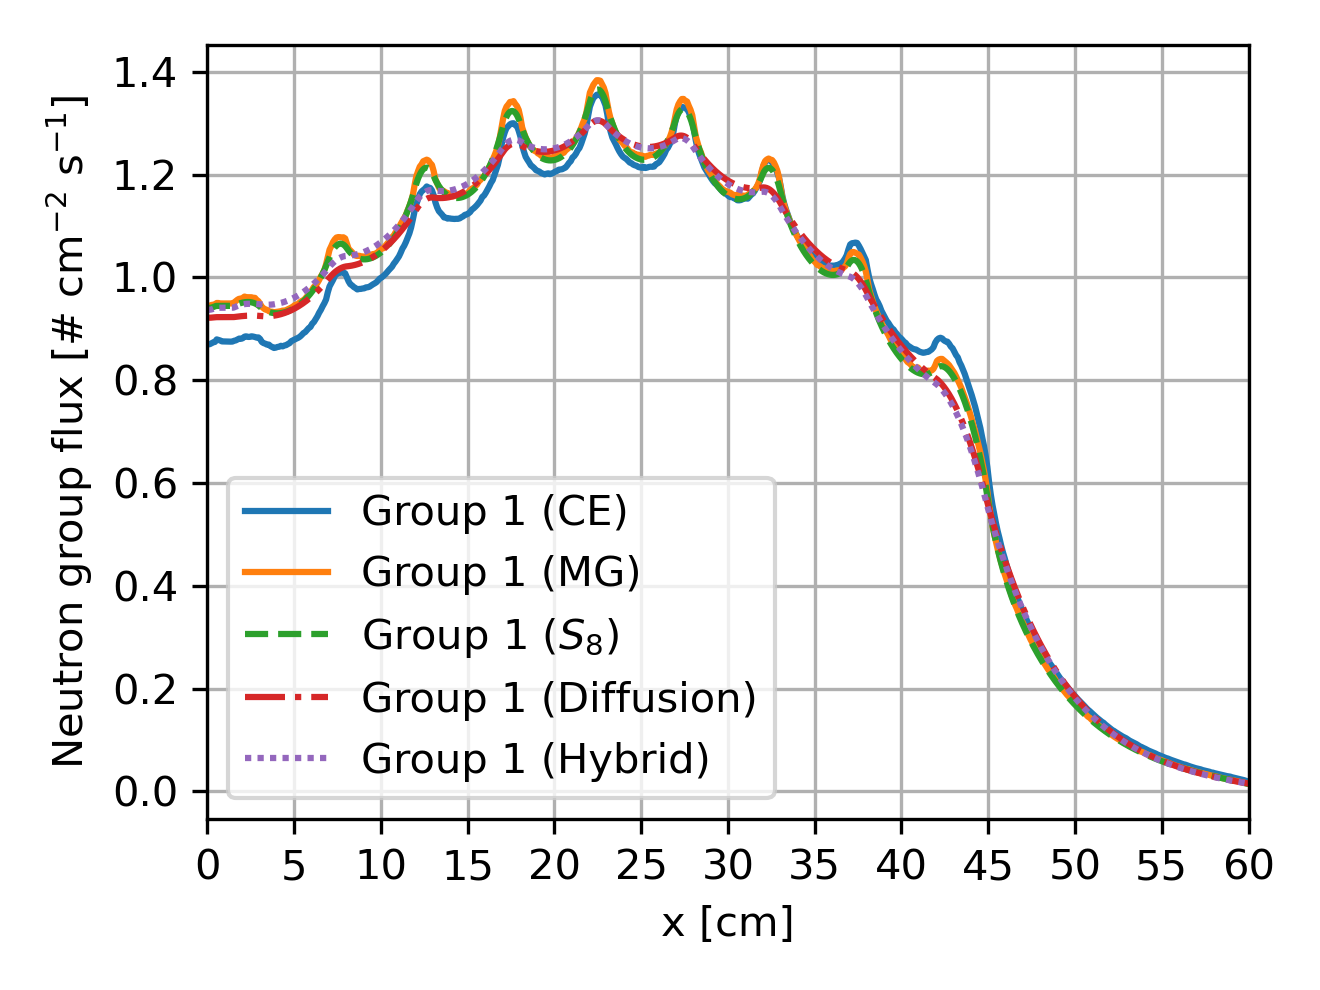
\includegraphics[width=\textwidth]{case-5a-group-1-flux}
    \caption{Group 1}
    \label{fig:c5ag1}
  \end{subfigure}
  \hfill
  \begin{subfigure}[t]{.49\textwidth}
    \centering
    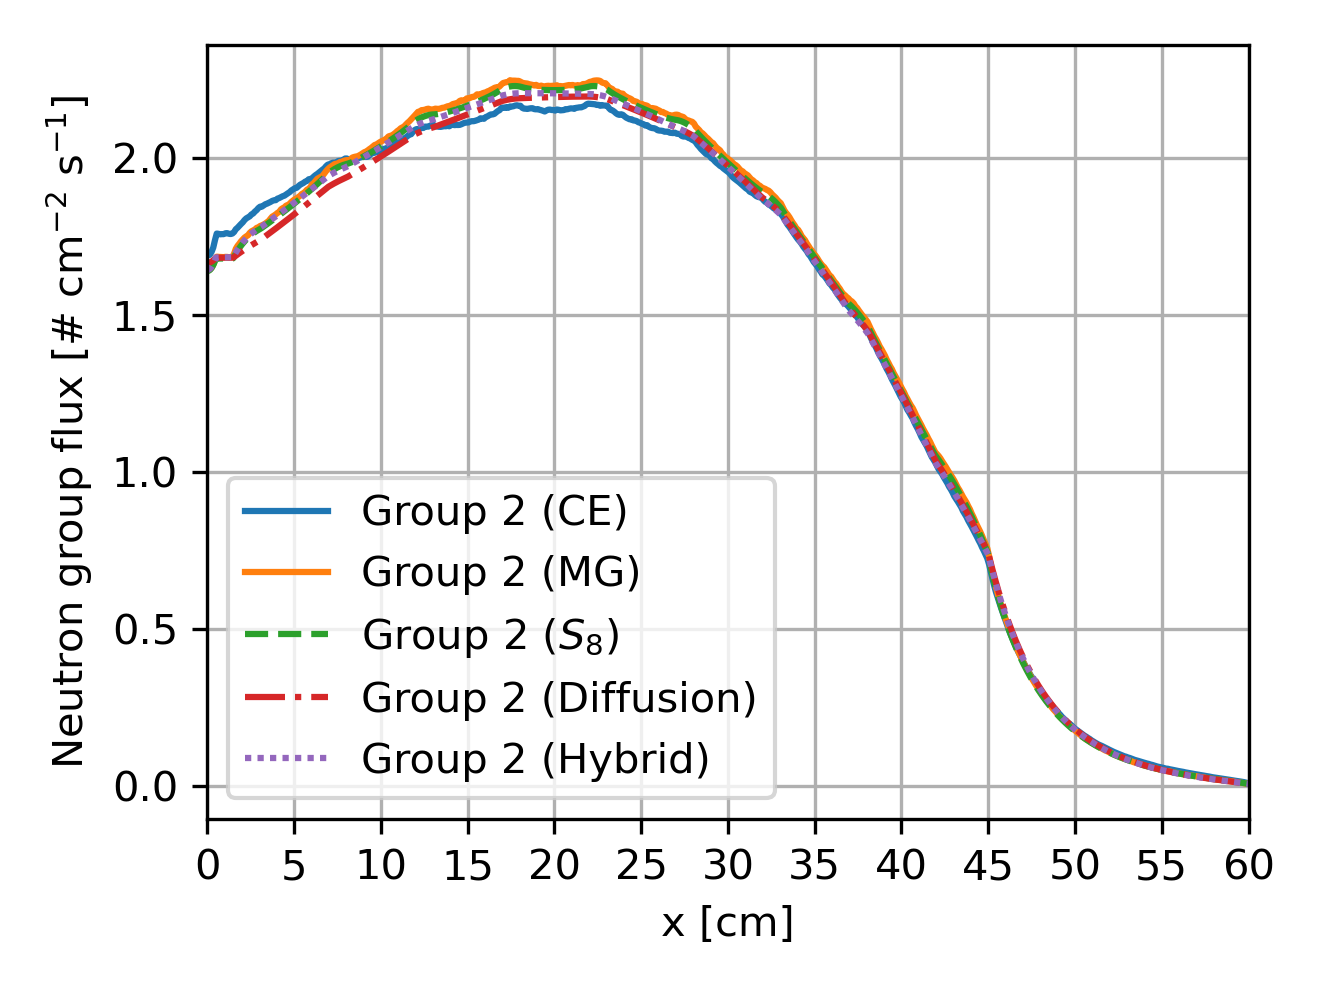
\includegraphics[width=\textwidth]{case-5a-group-2-flux}
    \caption{Group 2}
    \label{fig:c5ag2}
  \end{subfigure}
  \begin{subfigure}[t]{.49\textwidth}
    \centering
    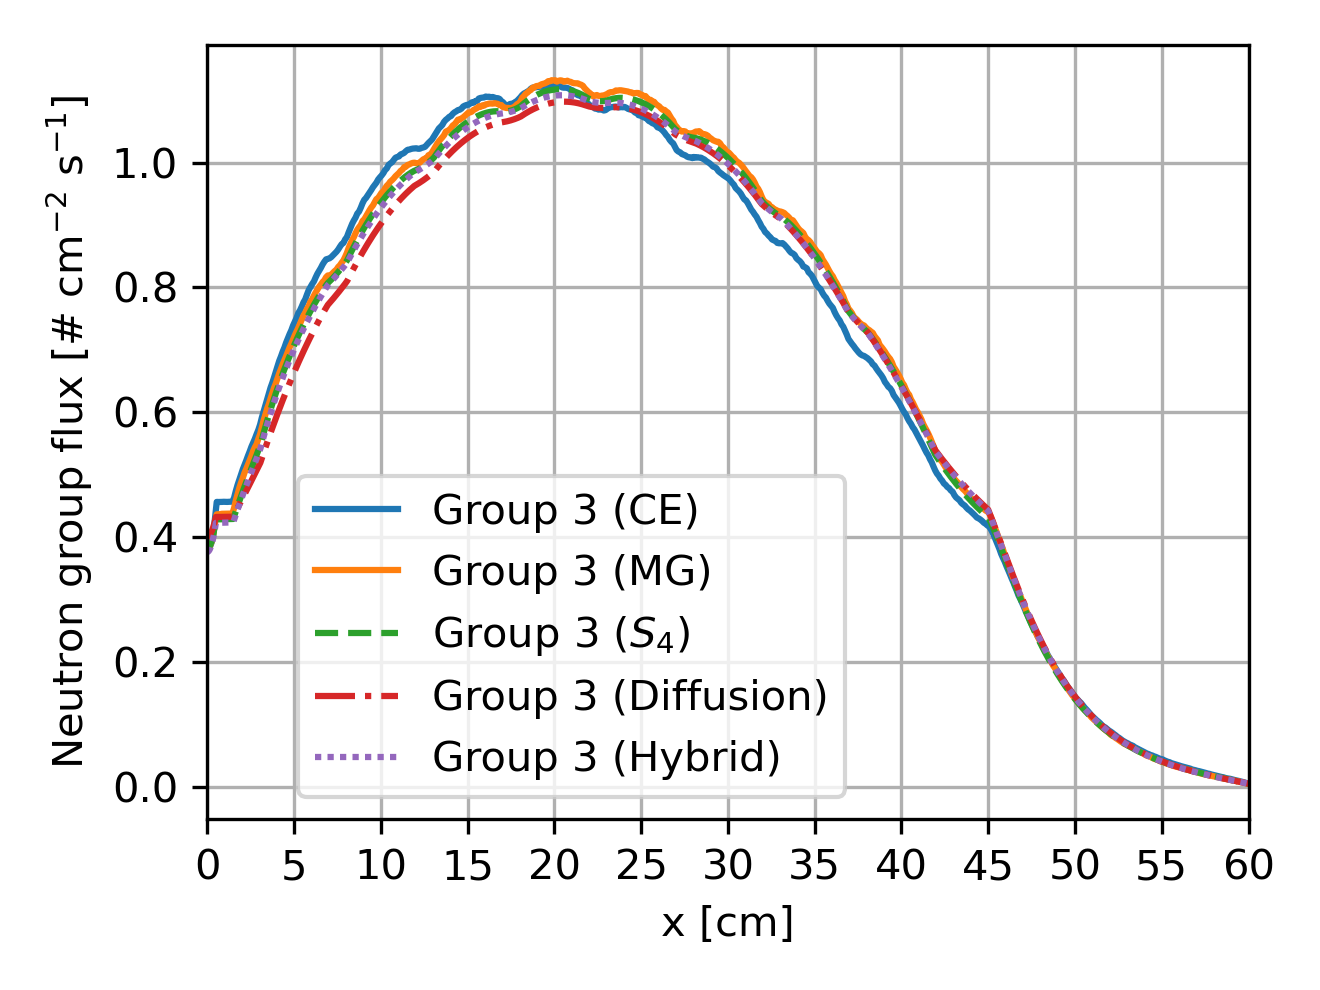
\includegraphics[width=\textwidth]{case-5a-group-3-flux}
    \caption{Group 3}
    \label{fig:c5ag3}
  \end{subfigure}
  \hfill
  \begin{subfigure}[t]{.49\textwidth}
    \centering
    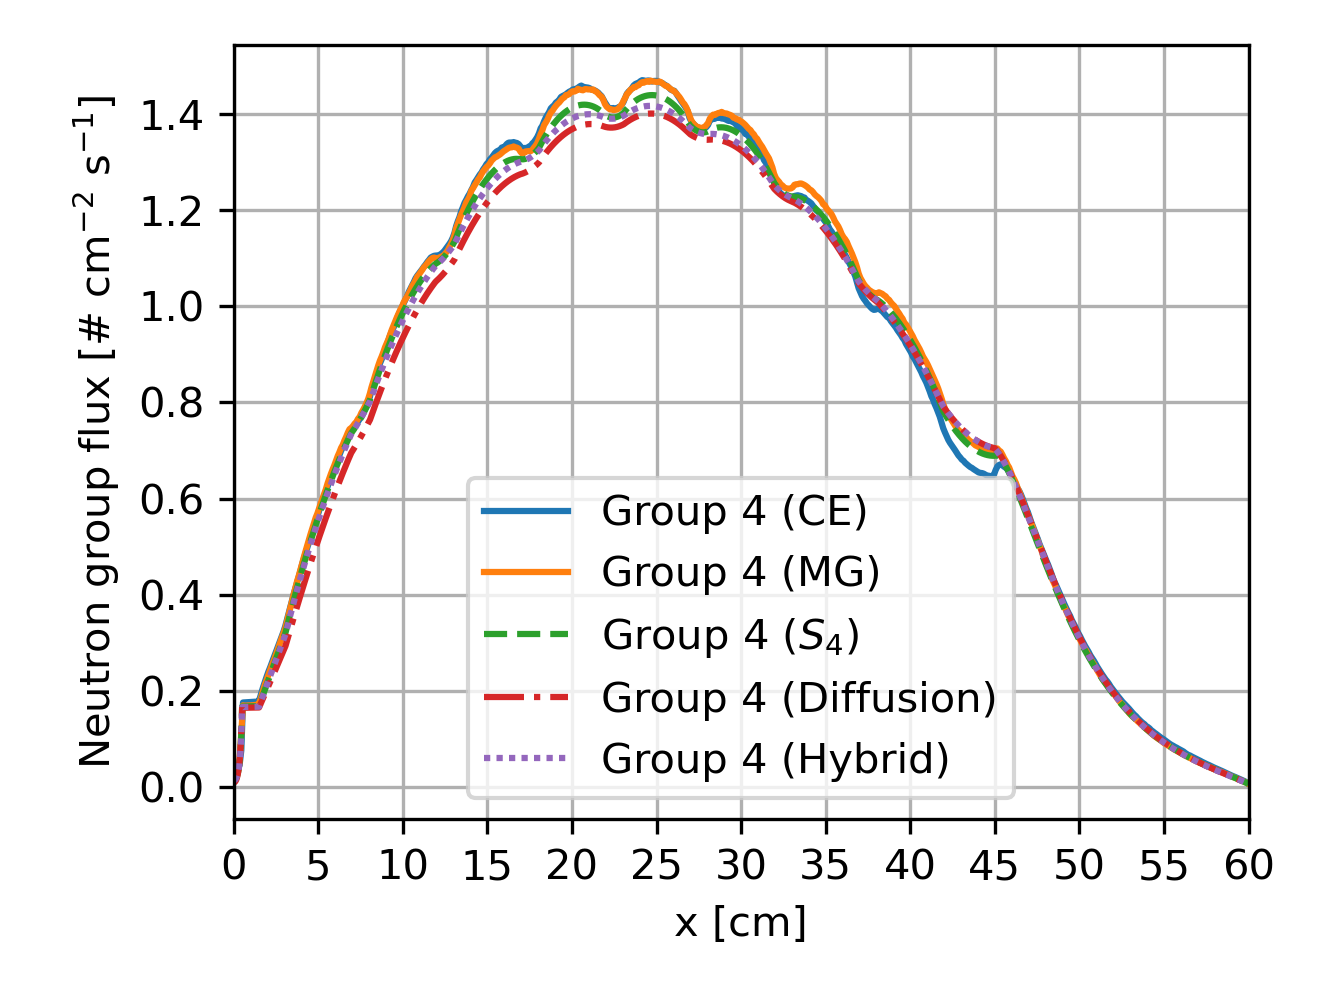
\includegraphics[width=\textwidth]{case-5a-group-4-flux}
    \caption{Group 4}
    \label{fig:c5ag4}
  \end{subfigure}
  \caption{Neutron group flux distributions for Case 5a from OpenMC-CE, OpenMC-MG, $S_8$, neutron
  diffusion, and hybrid methods.}
  \label{fig:c5aflux}
\end{figure}
%
\begin{figure}[htb!]
  \centering
  \begin{subfigure}[t]{.49\textwidth}
    \centering
    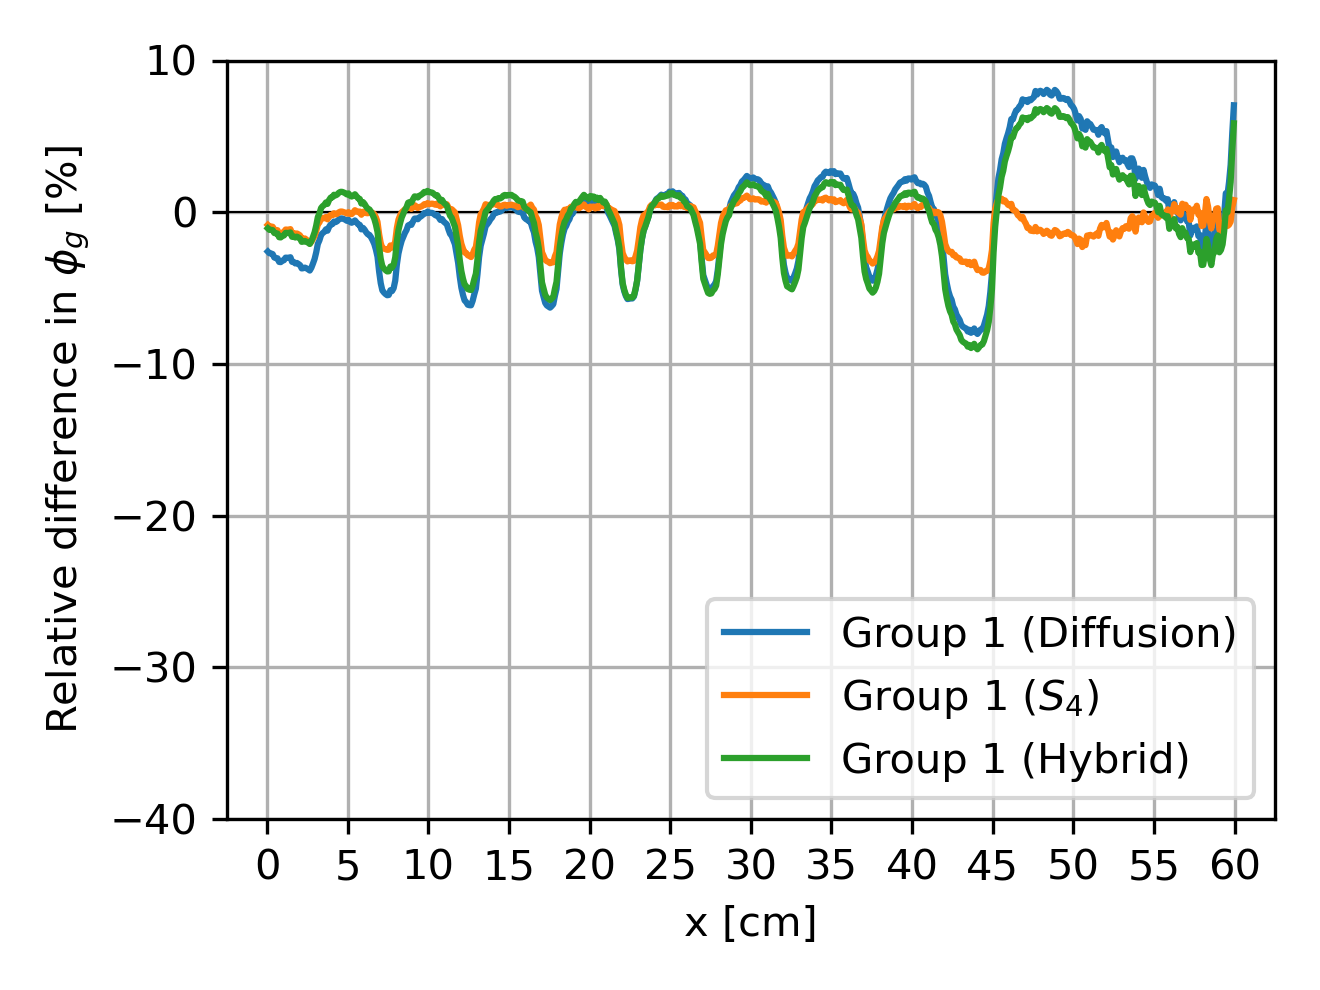
\includegraphics[width=\textwidth]{case-5a-group-1-flux-error}
    \caption{Group 1}
    \label{fig:c5ag1e}
  \end{subfigure}
  \hfill
  \begin{subfigure}[t]{.49\textwidth}
    \centering
    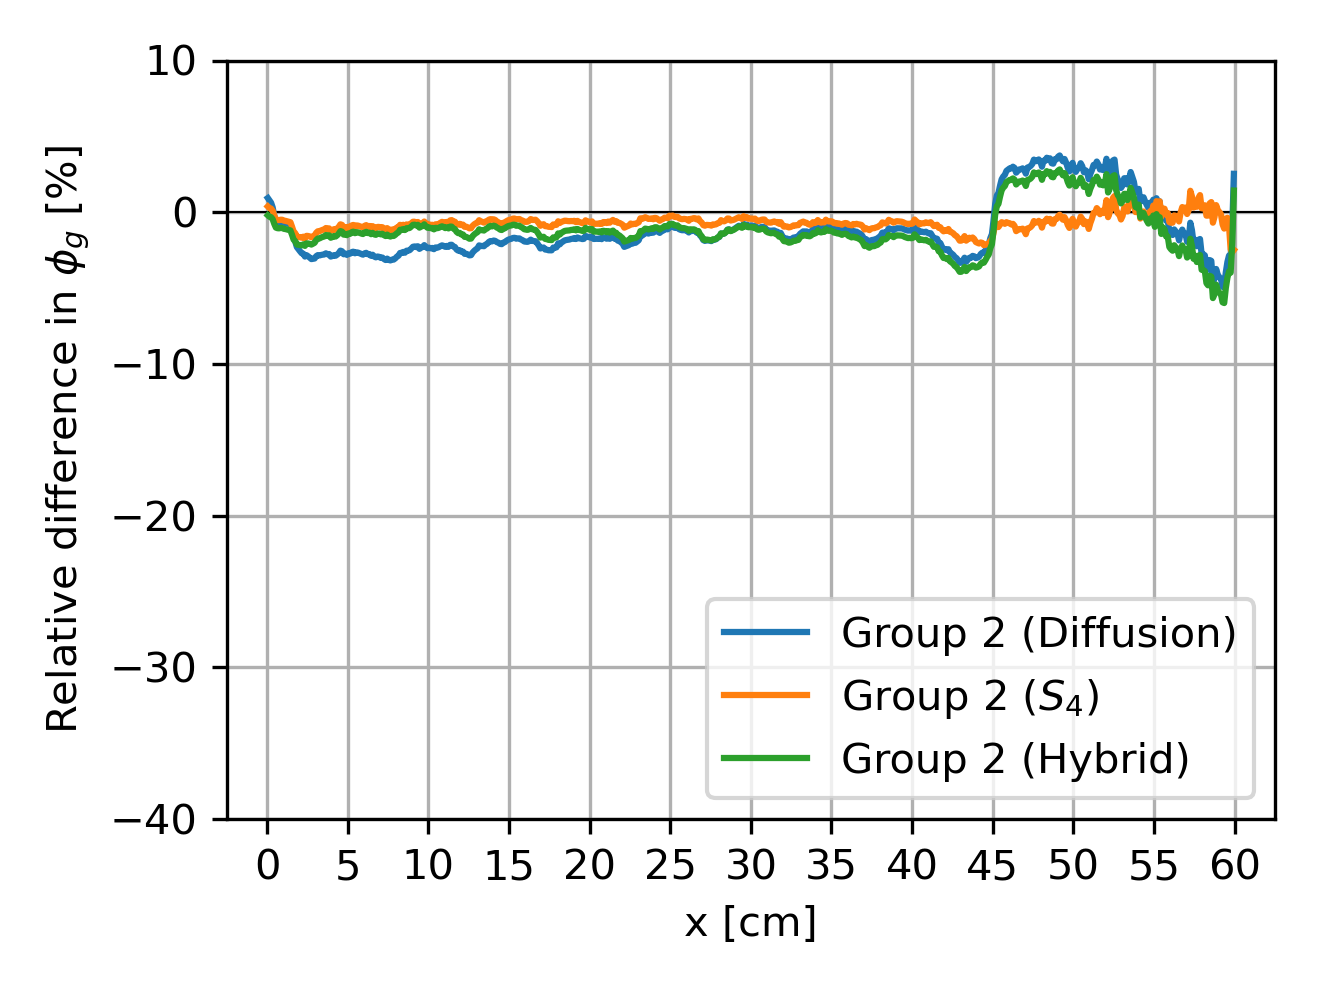
\includegraphics[width=\textwidth]{case-5a-group-2-flux-error}
    \caption{Group 2}
    \label{fig:c5ag2e}
  \end{subfigure}
  \begin{subfigure}[t]{.49\textwidth}
    \centering
    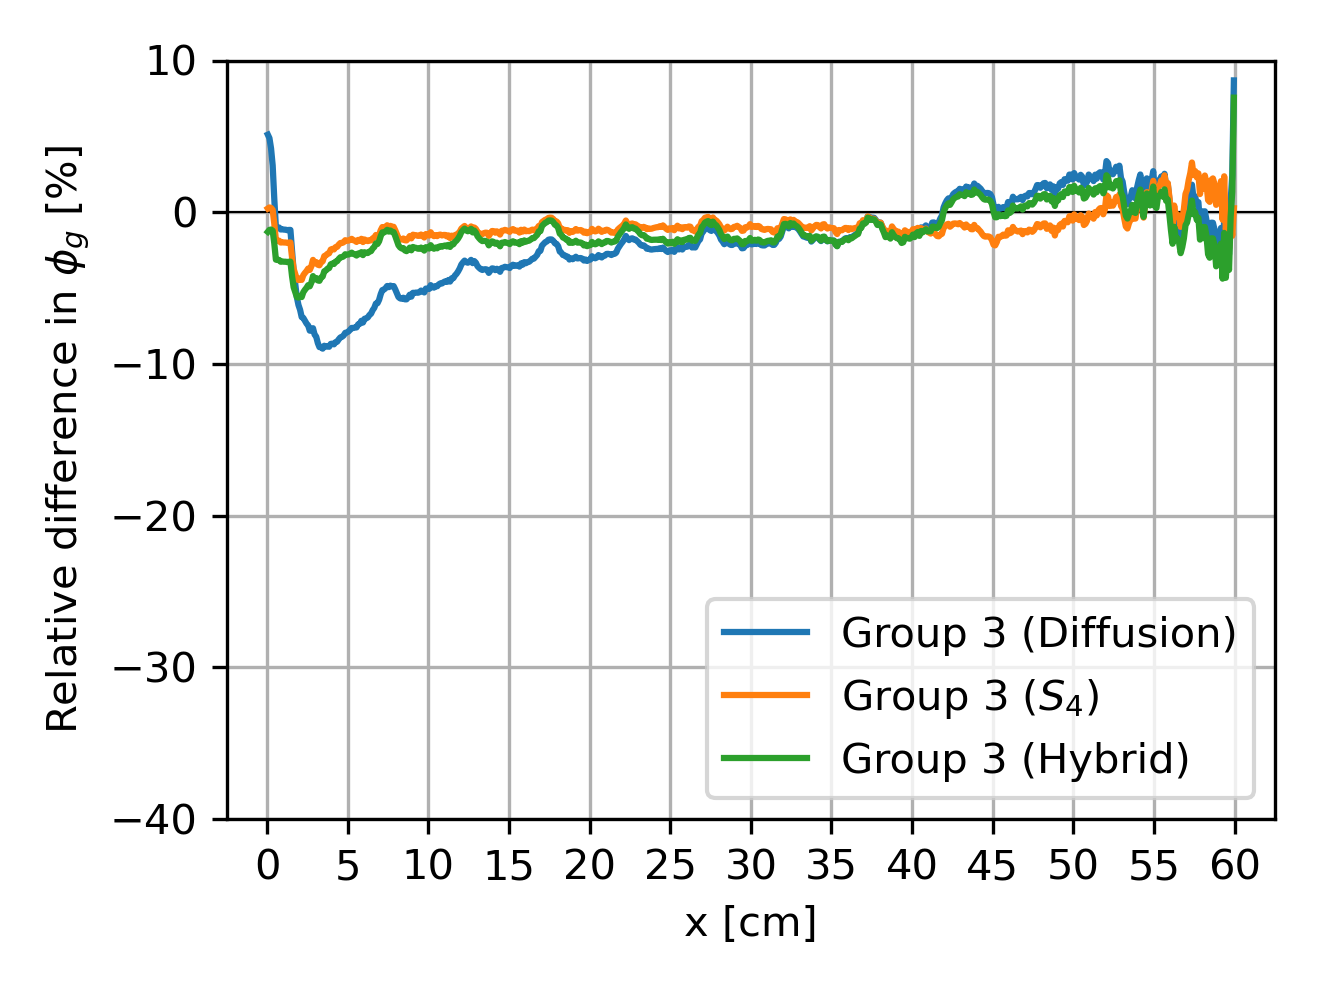
\includegraphics[width=\textwidth]{case-5a-group-3-flux-error}
    \caption{Group 3}
    \label{fig:c5ag3e}
  \end{subfigure}
  \hfill
  \begin{subfigure}[t]{.49\textwidth}
    \centering
    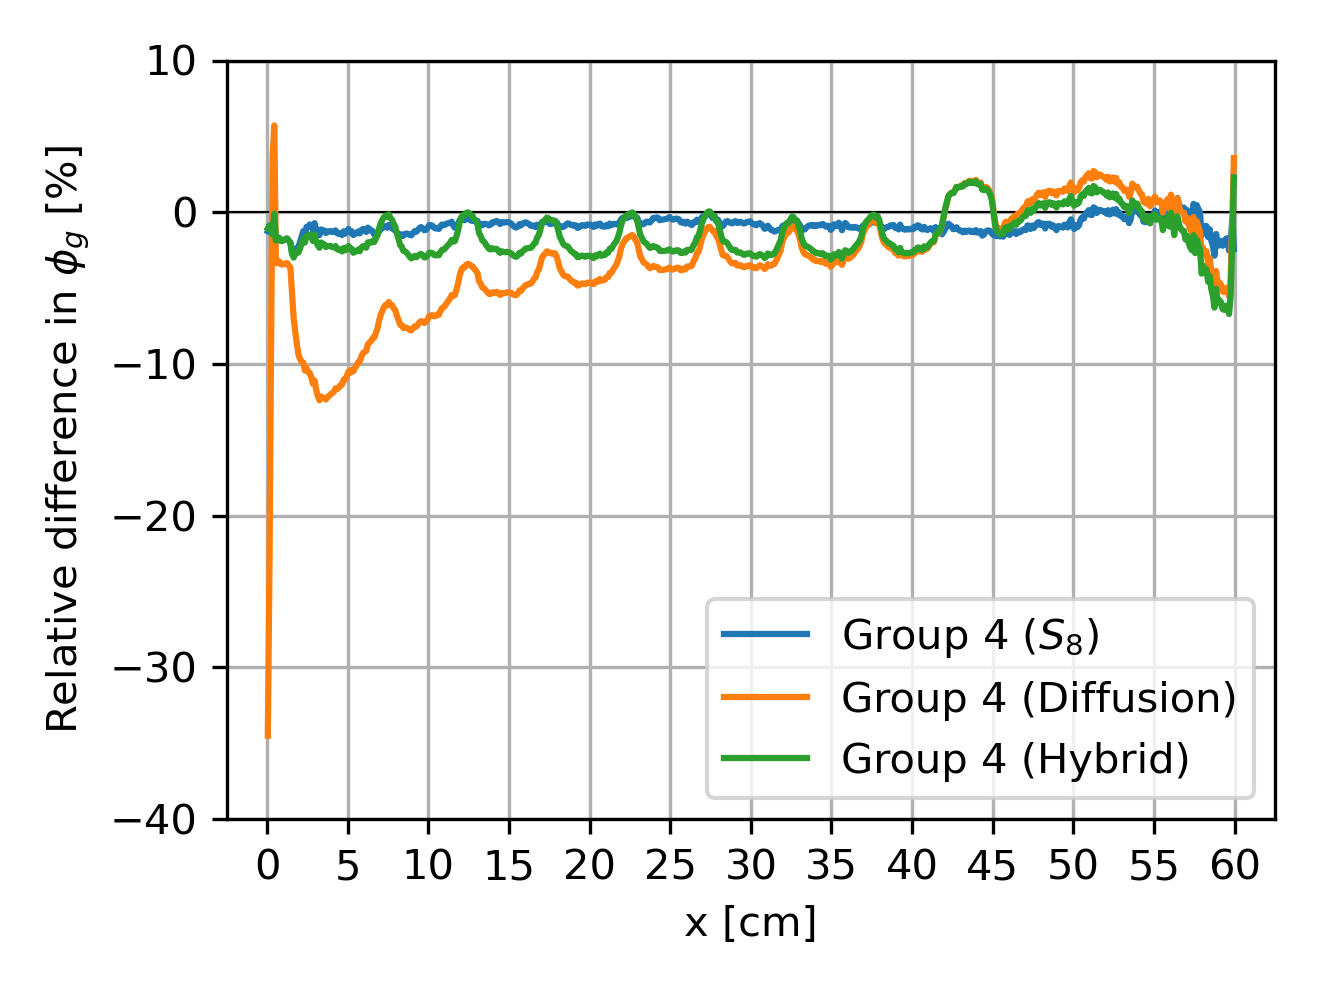
\includegraphics[width=\textwidth]{case-5a-group-4-flux-error}
    \caption{Group 4}
    \label{fig:c5ag4e}
  \end{subfigure}
  \caption{Relative differences of the neutron group flux distributions for Case 5a from the $S_8$,
    neutron diffusion, and hybrid methods with respect to OpenMC-MG.}
  \label{fig:c5afluxe}
\end{figure}
%
\begin{table}[tb!]
  \centering
  \footnotesize
  \caption{Normalized flux error $\varepsilon$ for Case 5a from the $S_8$, neutron diffusion, and
    hybrid methods with respect to OpenMC-MG.}
  \begin{tabular}{c S S S S}
    \toprule
    {\multirow{2}{*}{\textbf{Method}}} &
    \multicolumn{4}{c}{\textbf{Normalized flux error,} $\bm{\varepsilon_g}$} \\
    \cmidrule{2-5}
    & {\textbf{Group 1}} & {\textbf{Group 2}} & {\textbf{Group 3}} &
    {\textbf{Group 4}} \\
    \midrule
    $S_8$     & 0.0078 & 0.0074 & 0.0083 & 0.0085 \\
    Diffusion & 0.0305 & 0.0202 & 0.0313 & 0.0406 \\
    Hybrid    & 0.0290 & 0.0147 & 0.0143 & 0.0216 \\
    \bottomrule
  \end{tabular}
  \label{table:c5aerror}
\end{table}

\subsection{Correction Regions \& Diffusion Coefficients}

In this section, I compare the $P_1$-based diffusion coefficients, reference \glspl{SVDC}, and
hybrid \glspl{SVDC} for Cases 3b and 5a. As in Section \ref{sec:hybrid-method}, the reference
\glspl{SVDC} are derived from the $S_8$ flux solution, while the hybrid \glspl{SVDC} are derived
from the $S_8$ subsolver flux solution within the Hybrid $S_N$-Diffusion method.

Figure \ref{fig:c3bdiffcoef} shows the various diffusion coefficient distributions for Case 3b
between $x=0$ cm and $x=30$ cm. The figures omit the large diffusion coefficient values in the
air gap region between $x=0.5$ cm and $x=1$ cm since they do not show any significant features. The
hybrid \glspl{SVDC} closely match
the reference \gls{SVDC} within most of the correction region, which terminates at $x=20$ cm.

\begin{figure}[htb!]
  \centering
  \begin{subfigure}[t]{.49\textwidth}
    \centering
    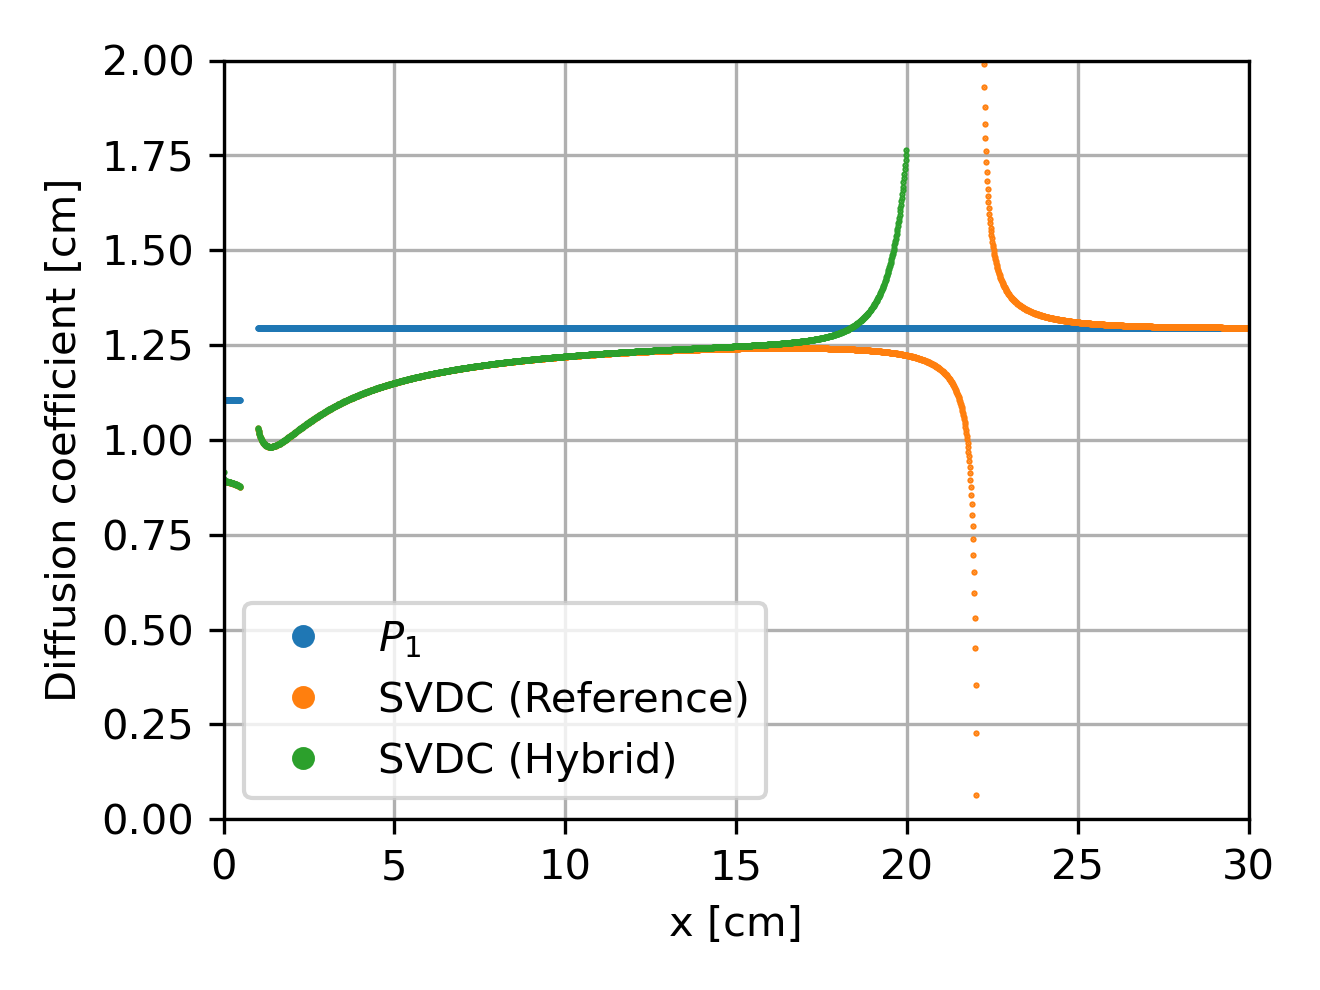
\includegraphics[width=\textwidth]{case-3b-group-1-diffcoef}
    \caption{Group 1}
    \label{fig:c3bg1dc}
  \end{subfigure}
  \hfill
  \begin{subfigure}[t]{.49\textwidth}
    \centering
    \includegraphics[width=\textwidth]{case-3b-group-2-diffcoef}
    \caption{Group 2}
    \label{fig:c3bg2dc}
  \end{subfigure}
  \begin{subfigure}[t]{.49\textwidth}
    \centering
    \includegraphics[width=\textwidth]{case-3b-group-3-diffcoef}
    \caption{Group 3}
    \label{fig:c3bg3dc}
  \end{subfigure}
  \hfill
  \begin{subfigure}[t]{.49\textwidth}
    \centering
    \includegraphics[width=\textwidth]{case-3b-group-4-diffcoef}
    \caption{Group 4}
    \label{fig:c3bg4dc}
  \end{subfigure}
  \caption{$P_1$-based diffusion coefficient, reference \gls{SVDC}, and hybrid \gls{SVDC}
    distributions for Case 3b between $x=0$ cm and $x=30$ cm.}
  \label{fig:c3bdiffcoef}
\end{figure}
%
\begin{figure}[htb!]
  \centering
  \includegraphics[width=.6\textwidth]{case-3b-grad-j}
  \caption{The gradient of current $J$ in the homogeneous fuel-graphite mixture from $x=1$ cm to
  $x=45$ cm for Case 3b.}
  \label{fig:c3bgradj}
\end{figure}

We recall that the hybrid method determines cutoff points within the correction region where the
\glspl{SVDC} coincide with the $P_1$-based diffusion coefficients so that the flux gradients
remain continuous. The hybrid method discards \glspl{SVDC} in the buffer region between this
cutoff point and the correction region boundary in favor of the $P_1$-based diffusion coefficients.
Notably, the group 1 reference \glspl{SVDC} (Figure \ref{fig:c3bg1dc}) only coincides
with the $P_1$-based diffusion coefficient after the vertical asymptotes where the flux
gradient approaches zero. The trends in group 1 reference \glspl{SVDC} before and after the
vertical asymptote imply that the \gls{SVDC} would have gradually approached the $P_1$-based
diffusion coefficient value if the asymptote did not exist. Determining the cutoff point for the
\glspl{SVDC} would have been problematic due to the vertical asymptote. However, the hybrid
\glspl{SVDC} coincide with the $P_1$-based diffusion coefficients before the vertical asymptote.
This behavior can be reliably reproduced in other geometries with large homogeneous fissile regions
(Cases 2a, 2b, and 3a) as long as the correction region terminates near the neutron flux peaks.
Nevertheless, the issue of handling vertical asymptotes in the \glspl{SVDC} has to be addressed
since flux peaks and troughs will inevitably occur in more realistic reactor geometries.

In contrast with the flux distributions in Figure \ref{fig:c3bflux}, the \gls{SVDC} distributions
suggest that the control rod contributes to an extended range of transport corrections on group 1
neutrons than the slower neutron groups. This phenomenon can be largely attributed to the highly
non-uniform fission neutron source distribution, which serves as the only source of group 1
neutrons in the absence of neutron up-scattering. The group 4 flux distribution
significantly influences on fission neutron source distribution, leading to more group 1 neutrons
being born closer to the reflector on the right than the
control rod on the left. The biased neutron source distribution induces a highly non-linear neutron
current distribution, as shown in Figure \ref{fig:c3bgradj}, and a departure from Fick's first law,
which relates the current to the flux gradient. Therefore, the \gls{SVDC} distributions show that
transport corrections to the faster neutron groups are as necessary for overall accuracy as
transport corrections to the slower neutron groups.

Figure \ref{fig:c5adiffcoef} shows the various diffusion coefficient distributions for Case 5a
between $x=0$ cm and $x=30$ cm. As with Case 3b, the figures omit the large diffusion coefficient
values in the air gap region between $x=0.5$ cm and $x=1.5$ cm  The hybrid \glspl{SVDC} closely match
the reference \gls{SVDC} within most of the correction region, which terminates at $x=10$ cm.

\begin{figure}[htb!]
  \centering
  \begin{subfigure}[t]{.49\textwidth}
    \centering
    \includegraphics[width=\textwidth]{case-5a-group-1-diffcoef}
    \caption{Group 1}
    \label{fig:c5ag1dc}
  \end{subfigure}
  \hfill
  \begin{subfigure}[t]{.49\textwidth}
    \centering
    \includegraphics[width=\textwidth]{case-5a-group-2-diffcoef}
    \caption{Group 2}
    \label{fig:c5ag2dc}
  \end{subfigure}
  \begin{subfigure}[t]{.49\textwidth}
    \centering
    \includegraphics[width=\textwidth]{case-5a-group-3-diffcoef}
    \caption{Group 3}
    \label{fig:c5ag3dc}
  \end{subfigure}
  \hfill
  \begin{subfigure}[t]{.49\textwidth}
    \centering
    \includegraphics[width=\textwidth]{case-5a-group-4-diffcoef}
    \caption{Group 4}
    \label{fig:c5ag4dc}
  \end{subfigure}
  \caption{$P_1$-based diffusion coefficient, reference \gls{SVDC}, and hybrid \gls{SVDC}
    distributions for Case 5a between $x=0$ cm and $x=30$ cm.}
  \label{fig:c5adiffcoef}
\end{figure}

Unlike Case 3b, the heterogeneous fuel-graphite lattice structure in Case 5a gives rise to
extreme fluctuations in the \gls{SVDC} distributions. The numerous asymptotes correspond to the
flux peaks and troughs throughout the lattice. Regardless, the presence of the control rod
suppresses the \gls{SVDC} fluctuations in the lattice close to the control rod, and the cutoff
points can be determined without manual intervention. The heterogeneous lattice induces competing
effects on the neutron flux, allowing for a smaller correction region of 10 cm in width. However,
the reduced correction region introduces less transport correction as a consequence.
Further investigation is needed to observe how the \gls{SVDC} distributions change with
increases in dimensionality for 2-D and 3-D systems.

\section{Summary} \label{sec:hybrid-summary}

In this chapter, I presented the theoretical basis for the Hybrid $S_N$-Diffusion method, a novel
two-level method for improving the neutron diffusion method for neutronics simulations of reactor
systems containing highly neutron-absorbing regions. The hybrid method relies on \glspl{SVDC}
derived from reference flux solutions of $S_N$ calculations to provide transport
corrections to the neutron diffusion method. The hybrid method is less computationally intensive
than the standalone $S_N$ neutron transport method because 1) $S_N$ calculations are limited to
correction regions which cover a fraction of the overall geometry, 2) and the \glspl{SVDC} are
observed to converge faster than the neutron fluxes in $S_N$ calculations.

I established a framework for the hybrid method for coupling an $S_N$ subsolver and a neutron
diffusion solver through outer iterations by taking advantage of the weak dependence of the $S_N$
flux solution on the approximate boundary conditions determined from the neutron diffusion flux
solution. This novel framework could be extended to improve multischeme methods, which
divide a problem domain into subdomains where different neutronics methods are applied. For
instance, in an $S_N$-diffusion multischeme method, the $S_N$ method is applied in subdomains with
significant transport effects while other subdomains are treated with the neutron diffusion method
to reduce the overall computational effort required \cite{wang_rattlesnake_2021}. 

I also developed an algorithm for identifying and discarding inaccurate \gls{SVDC} values, which
are expected to occur near the correction region boundary. I demonstrated the hybrid
method on 1-D graphite-moderated test cases modeled after the \gls{MSRE}. The hybrid method showed
good agreement with the reference Monte Carlo and $S_8$ methods after eliminating neutron energy
group discretization errors in test cases that included highly neutron-absorbing regions. The
hybrid method had better accuracy in more homogeneous systems largely due to the larger effective
transport correction regions through \glspl{SVDC}. Further work
is needed to extend and verify the hybrid method to 2-D and 3-D neutronics simulations and to
create a robust solution for determining \glspl{SVDC} around neutron flux peaks and troughs. 


\glsresetall

\chapter{Proposed Work}
\label{chap:proposedwork}
Chapter \ref{chap:intro} introduced the unique characteristics of liquid-fuel
\glspl{MSR}
and highlighted the challenges of modeling liquid-fuel \glspl{MSR}, particularly
with legacy software designed for solid-fuel reactors. In addition, Chapter
\ref{chap:lit} summarized and discussed existing \gls{MSR} multiphysics simulation tools and
their capabilities. In this discussion, I noted the lack of capabilities for modeling control rod
movement in multiphysics tools for \glspl{MSR}. Chapter \ref{chap:moltres} illustrated general
features and physics models in Moltres and summarized previous work done with
Moltres for multiphysics modeling of \glspl{MSR}. The latter sections detailed
several limitations in \gls{MSR} multiphysics modeling with
Moltres, including the need for further verification of
Moltres' capabilities, a turbulence model for simulating turbulent flow, and a
control rod modeling capability for transient simulations. In turn,
Chapter \ref{chap:benchmark} detailed a verification study of Moltres for fast-spectrum
\gls{MSR} modeling capabilities by evaluating its performance
through the CNRS benchmark and comparing its results against other
\gls{MSR} simulation tools. Lastly, Chapter \ref{chap:hybrid} presented the theory and preliminary
1-D results of the novel hybrid $S_N$-diffusion method for improved control rod modeling over
standard neutron diffusion methods.

In this chapter, I will detail the proposed work to further verify and validate Moltres' \gls{MSR}
modeling capabilities, and I will describe the further enhancements to Moltres that I will
implement to address the
need for enhanced turbulence modeling and control rod modeling in Moltres. The
proposed work contributes towards improving on Moltres' capabilities for
multiphysics modeling of \glspl{MSR} and, by extension, of advanced reactors.
Section \ref{sec:vv-study} details the proposed \gls{VV} study of Moltres based on the \gls{MSRE}
pump start-up and coast-down experiments. Section \ref{sec:turb} describes the proposed
implementation of a \gls{RANS}-based turbulence model in Moltres. Section \ref{sec:devel-hybrid}
describes the proposed development and implementation of the hybrid $S_N$-diffusion in Moltres.
Lastly, Section \ref{sec:devel-conclusion} summarizes the chapter and describes the research impact
of my proposed work on \gls{MSR} modeling.

\section{Verification \& Validation Study Based on the MSRE Pump Start-up and Coast-Down
Experiments} \label{sec:vv-study}

In addition to the completed verification study described in Chapter \ref{chap:benchmark}, I will
perform a \gls{VV} study of Moltres based on the \gls{MSRE} transient flow-rate tests,
consisting of fuel pump start-up and coast-down experiments at zero power criticality. The changing
flow rates cause changes to the \gls{DNP} distribution and the \gls{DNF} in the core. During both
experiments, the reactivity effects of \gls{DNP} drift were measured by
allowing the flux servo controller to maintain criticality. The controller maintains core
criticality by adjusting the control rod position in response to the reactivity effects. The
reactivity effect over time can be calculated by comparing the various control rod positions
(Figure \ref{fig:msre-trans}) with the control rod worth curve (Figure \ref{fig:msre-rod})
obtained during earlier experiments. I aim to
reproduce the calculated reactivity curve with a Moltres model of the \gls{MSRE}.

\begin{figure}[htb!]
  \centering
  \begin{minipage}[t]{.49\textwidth}
    \centering
    \includegraphics[width=\textwidth]{msre-transient}
    \caption{Control rod response to fuel pump start-up and coast-down
    \cite{prince_zero-power_1968}.}
    \label{fig:msre-trans}
  \end{minipage}
  \hfill
  \begin{minipage}[t]{.49\textwidth}
    \centering
    \includegraphics[width=\textwidth]{msre-rod-worth}
    \caption{Integral worth of control rod no. 1 \cite{prince_zero-power_1968}.}
    \label{fig:msre-rod}
  \end{minipage}
\end{figure}
%
\begin{figure}[htb!]
  \centering
  \includegraphics[width=.5\textwidth]{msre-2d}
  \caption{2-D axisymmetric model of the \gls{MSRE} to be used for the \gls{VV} study.}
  \label{fig:msre-2d}
\end{figure}

For this study, I will collaborate with Aaron Reynolds, the developer of QuasiMolto
\cite{reynolds_analysis_2023},
so that our software can be compared accurately. Therefore, Moltres
will be validated against \gls{MSRE} experimental data and verified against QuasiMolto simulation
results simultaneously. Both QuasiMolto and Moltres models of the \gls{MSRE} will be in R-Z
coordinates because QuasiMolto supports only 2-D R-Z \gls{MSR} modeling. Figure \ref{fig:msre-2d}
shows the 2-D axisymmetric model of the \gls{MSRE} that we intend to use
for this \gls{VV} study. The model omits the control rod in the \gls{MSRE}. Instead, we will
conduct $k$-eigenvalue calculations at every time-step to obtain the multiplication factor and
scale the \gls{DNP} source term. The salt flow speeds will be taken directly from available data in
the \gls{MSRE} report \cite{prince_zero-power_1968}. The datasets that we intend to compare between
QuasiMolto and Moltres for verification are:
%
\begin{itemize}
  \item Change in reactivity relative to the static (no flow) configuration over time during the
    pump start-up and coast-down transients
  \item Axial and radial neutron flux distributions of the static and steady-state (full flow)
    configurations
  \item Axial and radial \gls{DNP} distributions of the static and steady-state configurations
\end{itemize}

Since both QuasiMolto and Moltres will adopt the neutron diffusion method with the same flow
profile, we expect our results to be highly consistent with each other. We expect any discrepancies
between QuasiMolto and Moltres to be minor and due to differences in numerical discretization
schemes and routines. We will collaborate to eliminate errors arising from model misimplementation.

We also expect our reactivity data to be similar to the control rod response measured in Figure
\ref{fig:msre-trans}. However, our results are unlikely to match the experimental data exactly due
to known deficiencies in the physical \gls{MSRE} experimental setup and the simplifications we
adopted in our 2-D models. Among the model simplifications that we adopted, we expect the omission
of the upper and lower reactor plena to impact our results the most because the plena contain a
large volume of fuel salt above and below the fuel-graphite lattice. Therefore, as an extension, I
will consider exploring ways to include the plena in our models if our results deviate
significantly from the experimental data.

\section{Implementation of a RANS-Based Turbulence Model in Moltres} \label{sec:turb}

In Chapter \ref{chap:lit}, I presented requirements for \gls{MSR} modeling related to turbulence.
To address the current limitations, I will implement a Spalart-Allmaras turbulence model which
falls under the class of \gls{RANS}-based turbulence models. The
model will be implemented within the \gls{MOOSE} framework and
designed to be compatible with the fluid dynamics modeling infrastructure in
the existing \texttt{Navier-Stokes} module. This approach leverages the
advanced finite-element solver and multiphysics coupling capabilities in
\gls{MOOSE}.

I will
focus on verifying and validating its performance under specific flow conditions expected in
liquid-fuel \glspl{MSR}: wall-bounded turbulent flow with flow separation past
sharp changes in the flow channel geometry. The backward-facing step is a
widely known fluid dynamics problem commonly used to assess the accuracy of
turbulence model solvers \cite{lasher_computation_1992}.
The problem domain features a straight duct
on the left followed by a sudden back step in the lower wall which causes flow
separation. The flow eventually reattaches to the wall further downstream.
I will simulate and validate against experimental data from Driver \&
Seegmiller \cite{driver_features_1985}. The quantities of interest from their data that I plan to
use are the spatial distributions of the velocity components, turbulent
kinetic energy, and eddy viscosity, and the reattachment length of the
turbulent shear layer.

Potential issues that I may face include the lack of a crosswind diffusion stabilization scheme in
\gls{MOOSE} and the fact that local mass conservation is not guaranteed when modeling the
Navier-Stokes equations using the \gls{FEM} without special treatment. If these issues prove to be
insurmountable within a reasonable time frame, I will focus my efforts on adopting the mixing
length turbulence models currently available in \gls{MOOSE} or two-equation models which are in
active development with the recent \gls{FVM} implementation in \gls{MOOSE}. In this alternate
scenario, I will explore demonstrating coupled neutronics/thermal-hydraulics simulations with
turbulent flow modeling of the \gls{MSFR}.

\section{Development of a Novel Hybrid Method to Improve Control Rod Modeling in Moltres}
\label{sec:devel-hybrid}

In Chapter \ref{chap:hybrid}, I presented the theory and preliminary results of the hybrid
$S_N$-diffusion method for several 1-D \gls{MSRE}-inspired, graphite-moderated geometries. The
hybrid method generates \glspl{SVDC}, which provide pointwise corrections to the diffusion
sub-solver from
the $S_N$ sub-solver neutron current and flux gradient solutions. The hybrid method minimizes
computational costs by imposing the $S_N$ calculations on a small subdomain centered on the control
rod region and relaxing the $S_N$ sub-solver convergence tolerance since the neutron current and
flux gradient converges faster than the neutron flux. As intended,
the hybrid method provided better multiplication factor and neutron flux estimates over the
standard neutron diffusion method in systems containing strongly neutron-absorbing control rods.

In this section, I present a detailed description of the proposed work for the development and
implementation of the hybrid method in Moltres, the verification of the hybrid method against
reference OpenMC neutronics calculations, and the computational performance characterization of the
hybrid method.

\subsection{Development \& Implementation of the Hybrid Method}

The preliminary investigations in Chapter \ref{chap:hybrid} brought up three issues to be
addressed for the continued development of the hybrid $S_N$-diffusion method. The first issue
surrounds resolving \glspl{SVDC} near neutron flux peaks and troughs. The existing formulation
for \glspl{SVDC} in Eq. \ref{eq:svdc} are undefined at flux peaks and troughs due to division by
the flux gradient. I will explore alternative formulations to address this issue. For instance,
Tomatis \& Dall'Osso \cite{tomatis_application_2011} developed the formulation in Eq.
\ref{eq:tomatis} to address the same issue in their implementation of the Ronen method. Eq.
\ref{eq:tomatis} calculates corrections to the neutron streaming terms as additive
$\delta J$ terms. I will evaluate whether their formulation can be adapted to the hybrid
$S_N$-diffusion method. Otherwise, I plan to investigate similar additive correction formulations
for the hybrid $S_N$-diffusion method.

The second issue concerns the evaluation of appropriate correction regions and buffer zones for the
hybrid method. The correction region represents the problem domain of the $S_N$ sub-solver. It must
be large enough to provide sufficient transport correction in regions heavily influenced by the
control rod and to accommodate the discarding of inaccurate \glspl{SVDC} expected near the
boundary. I will investigate various test cases in 2-D and 3-D, similar to my preliminary work in
this report, to identify how various geometrical and material properties affect the minimum
required size of the correction region. For instance, my preliminary work showed that the
geometrical heterogeneity and optical thickness strongly affects the \gls{SVDC} distributions,
which are a measure of the amount of transport correction required. With my expected findings, I
will generate a set of criteria for determining the appropriate correction region size for a given
reactor geometry.

The last issue concerns the automatic evaluation of buffer zones which are regions near the
boundaries of the correction region where inaccurate \glspl{SVDC} are discarded. For the 1-D
problems, I set up an outward sweeping algorithm that compares the \glspl{SVDC} with the default
$P_1$-based diffusion coefficients. The implementation of this sweeping algorithm is less clear for
2-D and 3-D problems which feature more than two angular directions. I will tackle this issue
in conjunction with the second issue by analyzing the \gls{SVDC} distributions obtained from
2-D and 3-D test cases.

Naturally, the implementation and extension of the hybrid method in Moltres for 2-D and 3-D
modeling must precede my attempts at resolving the second and third issue. I will implement the
$S_N$ method with diffusion synthetic acceleration in Moltres or as a separate MOOSE-based
application. I will also implement supporting features for the coupling the $S_N$ solver with the
existing diffusion solver to run the hybrid method.

\subsection{Verification of the Hybrid Method}

I will verify the hybrid method against reference OpenMC calculations with several test cases
similar to the 1-D test cases in Chapter \ref{chap:hybrid}. The test cases will be various 2-D
and 3-D representations of \gls{MSRE}-inspired models with the fuel-graphite lattice, the control
rod, the air-filled rod guide tube, and reflectors. The verification study will include
permutations of the following factors:
%
\begin{itemize}
  \item Dimensionality (e.g, 2-D, 3-D)
  \item Geometrical symmetries and asymmetries related to the control rod position
  \item Static control rods at various levels of insertion
  \item Control rod material composition
\end{itemize}

\subsection{Computational Performance Characterization of the Hybrid Method}

I intend for the hybrid $S_N$-diffusion method to be tractable on small computing clusters for
time-dependent multiphysics simulations. Therefore, I will characterize the computational
performance of the hybrid method and compare it against the standard $S_N$ and neutron diffusion
methods. I expect the hybrid method to be faster than the standard $S_N$ method due to the small
correction region size relative to the full reactor geometry and the faster convergence of
\glspl{SVDC} relative to the neutron flux in the hybrid $S_N$ sub-solvers. I plan to perform the
characterization with some of the 2-D and 3-D verification study test cases.

In addition, I will evaluate the hybrid method's parallel scaling performance to identify potential
performance bottlenecks in the implementation. Good parallel scaling performance is essential for
leveraging on computational resources for large reactor simulations. I will run both weak and
strong scaling studies using some of the 2-D and 3-D test cases for this evaluation.

\section{Conclusion} \label{sec:devel-conclusion}

In this chapter, I detailed the proposed work to verify and validate Moltres' existing capabilities
for modeling \gls{DNP} drift and out-of-core decay in \glspl{MSR}, implement a \gls{RANS}-based
turbulence model in Moltres, and develop a hybrid $S_N$-diffusion method for improved control
rod modeling in Moltres. My work will extend the applicability of Moltres for a wider range of
MSR safety analyses involving turbulent flow and control rod effects. Most notably, the hybrid
method will enable Moltres users to run time-dependent multiphysics \gls{MSR} simulations with
control rod movement and address this technical gap in the existing literature. Through my work on
the hybrid method, I will also characterize and provide insights on neutron transport effects in
\gls{MSR} that are neglected by the neutron diffusion method.

\glsresetall

\backmatter

\bibliographystyle{ieeetr}
\bibliography{bibliography}

\end{document}
\endinput
%%
